\documentclass[]{final_report}
\usepackage{graphicx}
\usepackage{hyperref}
\usepackage{titlesec}
\usepackage[utf8]{inputenc}
\usepackage[backend=biber, style=ieee]{biblatex}
\usepackage{amsmath}
\usepackage{amssymb}
\usepackage{float}
\usepackage{tabularx} % Needed for the X column type
\usepackage{booktabs} % For prettier tables
\usepackage{lipsum}   % For dummy text
\usepackage{mathtools}
\usepackage{stmaryrd}
\usepackage{mdframed}
\usepackage{caption}
\usepackage{array}
\usepackage{listings}
\usepackage[dvipsnames]{xcolor}
\usepackage{adjustbox}
\usepackage{longtable}
\usepackage{tikz}
\usepackage{rotating}
\usepackage{pdflscape}
\usepackage{fancyhdr}
\usepackage{comment}
\usepackage{multirow}
\usepackage{lscape} % Use lscape package instead of pdflscape
\usepackage{afterpage} % Required for \afterpage command
\usepackage{fancyhdr} % Required for custom headers and footers
\usepackage{everypage}
\usepackage{url}





\addbibresource{fyp.bib}
\usepackage{amsthm}

%%%%%%%%%%%%%%%%%%%%%%
%%% Input project details
\def\studentname{Jude Asare}
\def\reportyear{2024}
\def\projecttitle{User Manual: Digital Signature Benchmarking Application}


\def\fullOrHalfUnit{User Manual} 


\begin{document}





%%%%%%%%%%%%%%%%%%%%%%
%%% Table of Contents
\tableofcontents\pdfbookmark[0]{Table of Contents}{toc}\newpage



\chapter{Installation and Run instructions}

\section*{Prerequisites:} Java must be installed to run this application

\section*{Demo Videos:}
The following is the demo for the application, not inclusive of the additional features that can be found in this user manual:

Demo link: \url{https://youtu.be/5DHMEd1Vkok}


\section*{Running the application}

To run the application, using the provided jar, run the following from a command line:

\begin{verbatim}
java -jar digital-signature-benchmarking-1.0.jar
\end{verbatim}



%%%%%%%%%%%%%%%%%%%%%%
%%% Introduction
\chapter{Introduction}

The application comprises four main portals, each linked to functionalities essential for facilitating digital signatures. These portals allow transition between standard and benchmarking-specific operations.
\begin{enumerate}
    \item \textbf{Main Menu:} The gateway to key and signature functionalities within the application.
    \item \textbf{Key Generation:} Allows generation of RSA key pairs, either singularly for standard operations or in batches for benchmarking purposes.
    \item \textbf{Signature Creation:} Facilitates creation of individual signatures in standard mode or signature batches in benchmarking mode for deterministic signature types.
    \item \textbf{Signature Verification:} Enables validation of individual or batch signatures against messages or message batches, respectively, in standard or benchmarking modes.
\end{enumerate}

The application offers four modalities, categorised into standard mode and a suite of benchmarking modes (including Benchmarking (default), Comparison Benchmarking, and Custom Comparison Benchmarking). 

\textbf{Standard Mode}: Activated by switching off the benchmarking toggle switch for any application portal and allows for performing singular operations whose performance is not recorded.

\textbf{Benchmarking Modalities}

\begin{itemize}
    \item \textbf{Normal Benchmarking}: The system provides a straightforward assessment of the relevant process, offering the user key-specific benchmarking results. For signature operations, the same hash function is applied to every key configuration.
        \item \textbf{Comparison Benchmarking (Standard vs. Provably Secure)}: This mode offers a direct comparative analysis between standard and provably secure key configuration groups (with user selected hash functions for each group). This allows evaluation of the performance of the Standard and Provably Secure groupings, with all trials repeated for every hash function and key configuration combination for each group. Results are then presented side by side in a table and/or overlaid graphs for each entered key size. 
     \item \textbf{Custom Comparison Benchmarking}: In this mode, users have the flexibility to specify key configurations and corresponding hash functions for each group. They can then assess the performance of their chosen key configuration groupings, with all trials repeated for every hash function and key configuration combination for each group. Results are presented side by side in a table and/or overlaid graphs for each entered key size.
\end{itemize}


\chapter{Main Menu}


\begin{figure}[H]
    \centering
    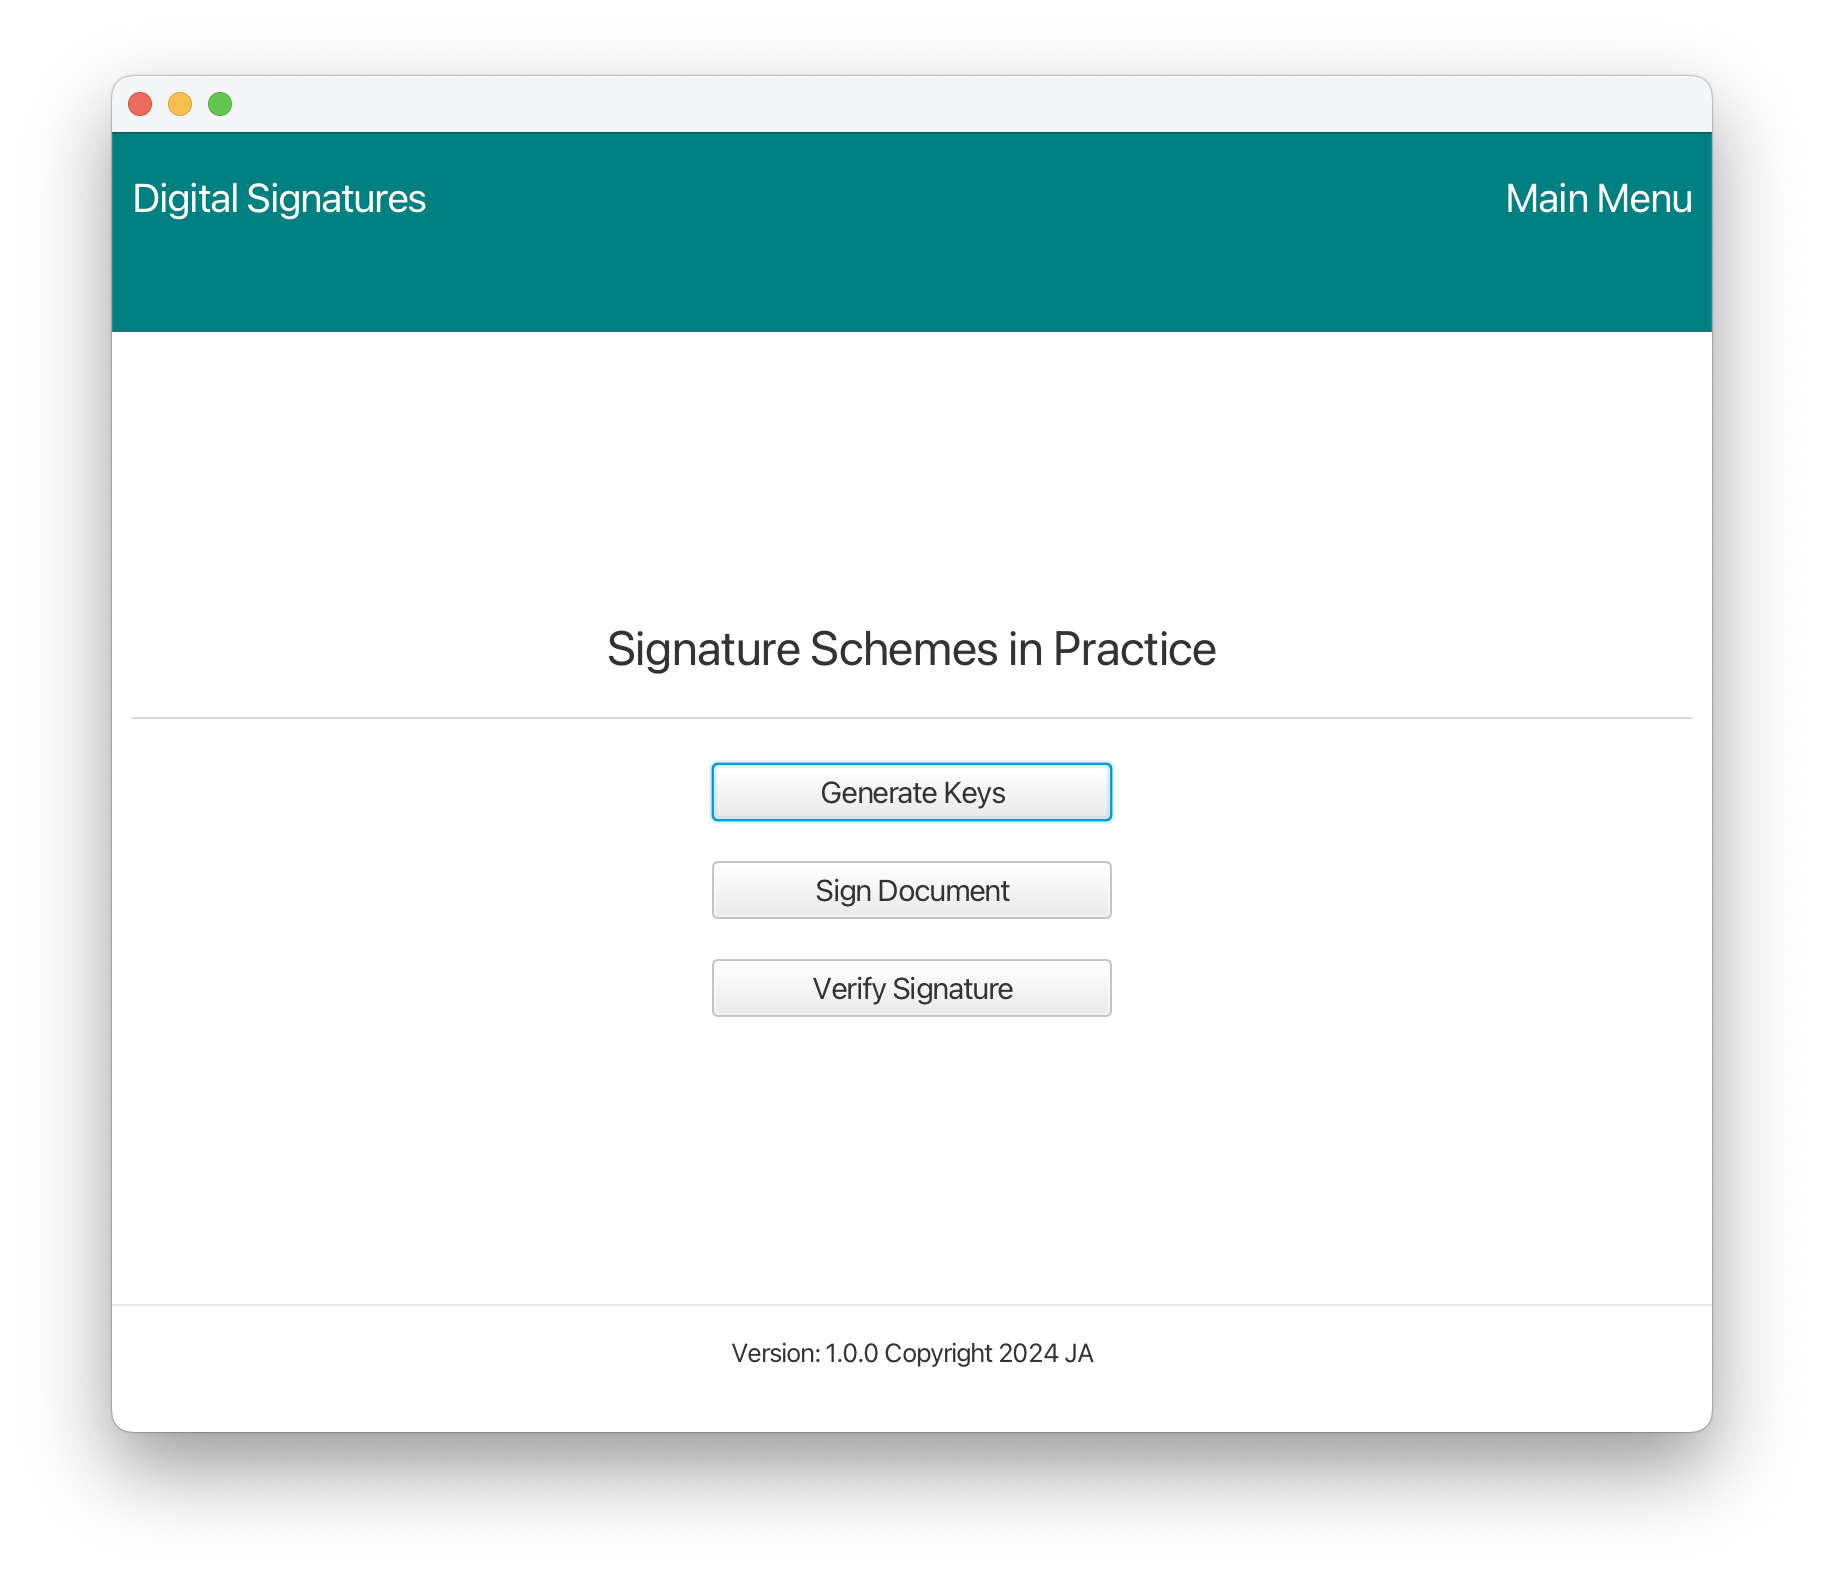
\includegraphics[scale=0.4]{main_pictures/ui/mainMenu.png}
   \caption{Comparison Benchmarking: Main Menu}
\end{figure}
The main menu screen of the application presents a straightforward and functional layout, serving as the gateway to its core features via menu buttons. 


\chapter{Benchmarking Mode}
\subsection{Key Generation}
\begin{figure}[H]
    \centering % Center the images
    
    % First image in a minipage
    \begin{minipage}{0.495\textwidth}
        \centering
        \fbox{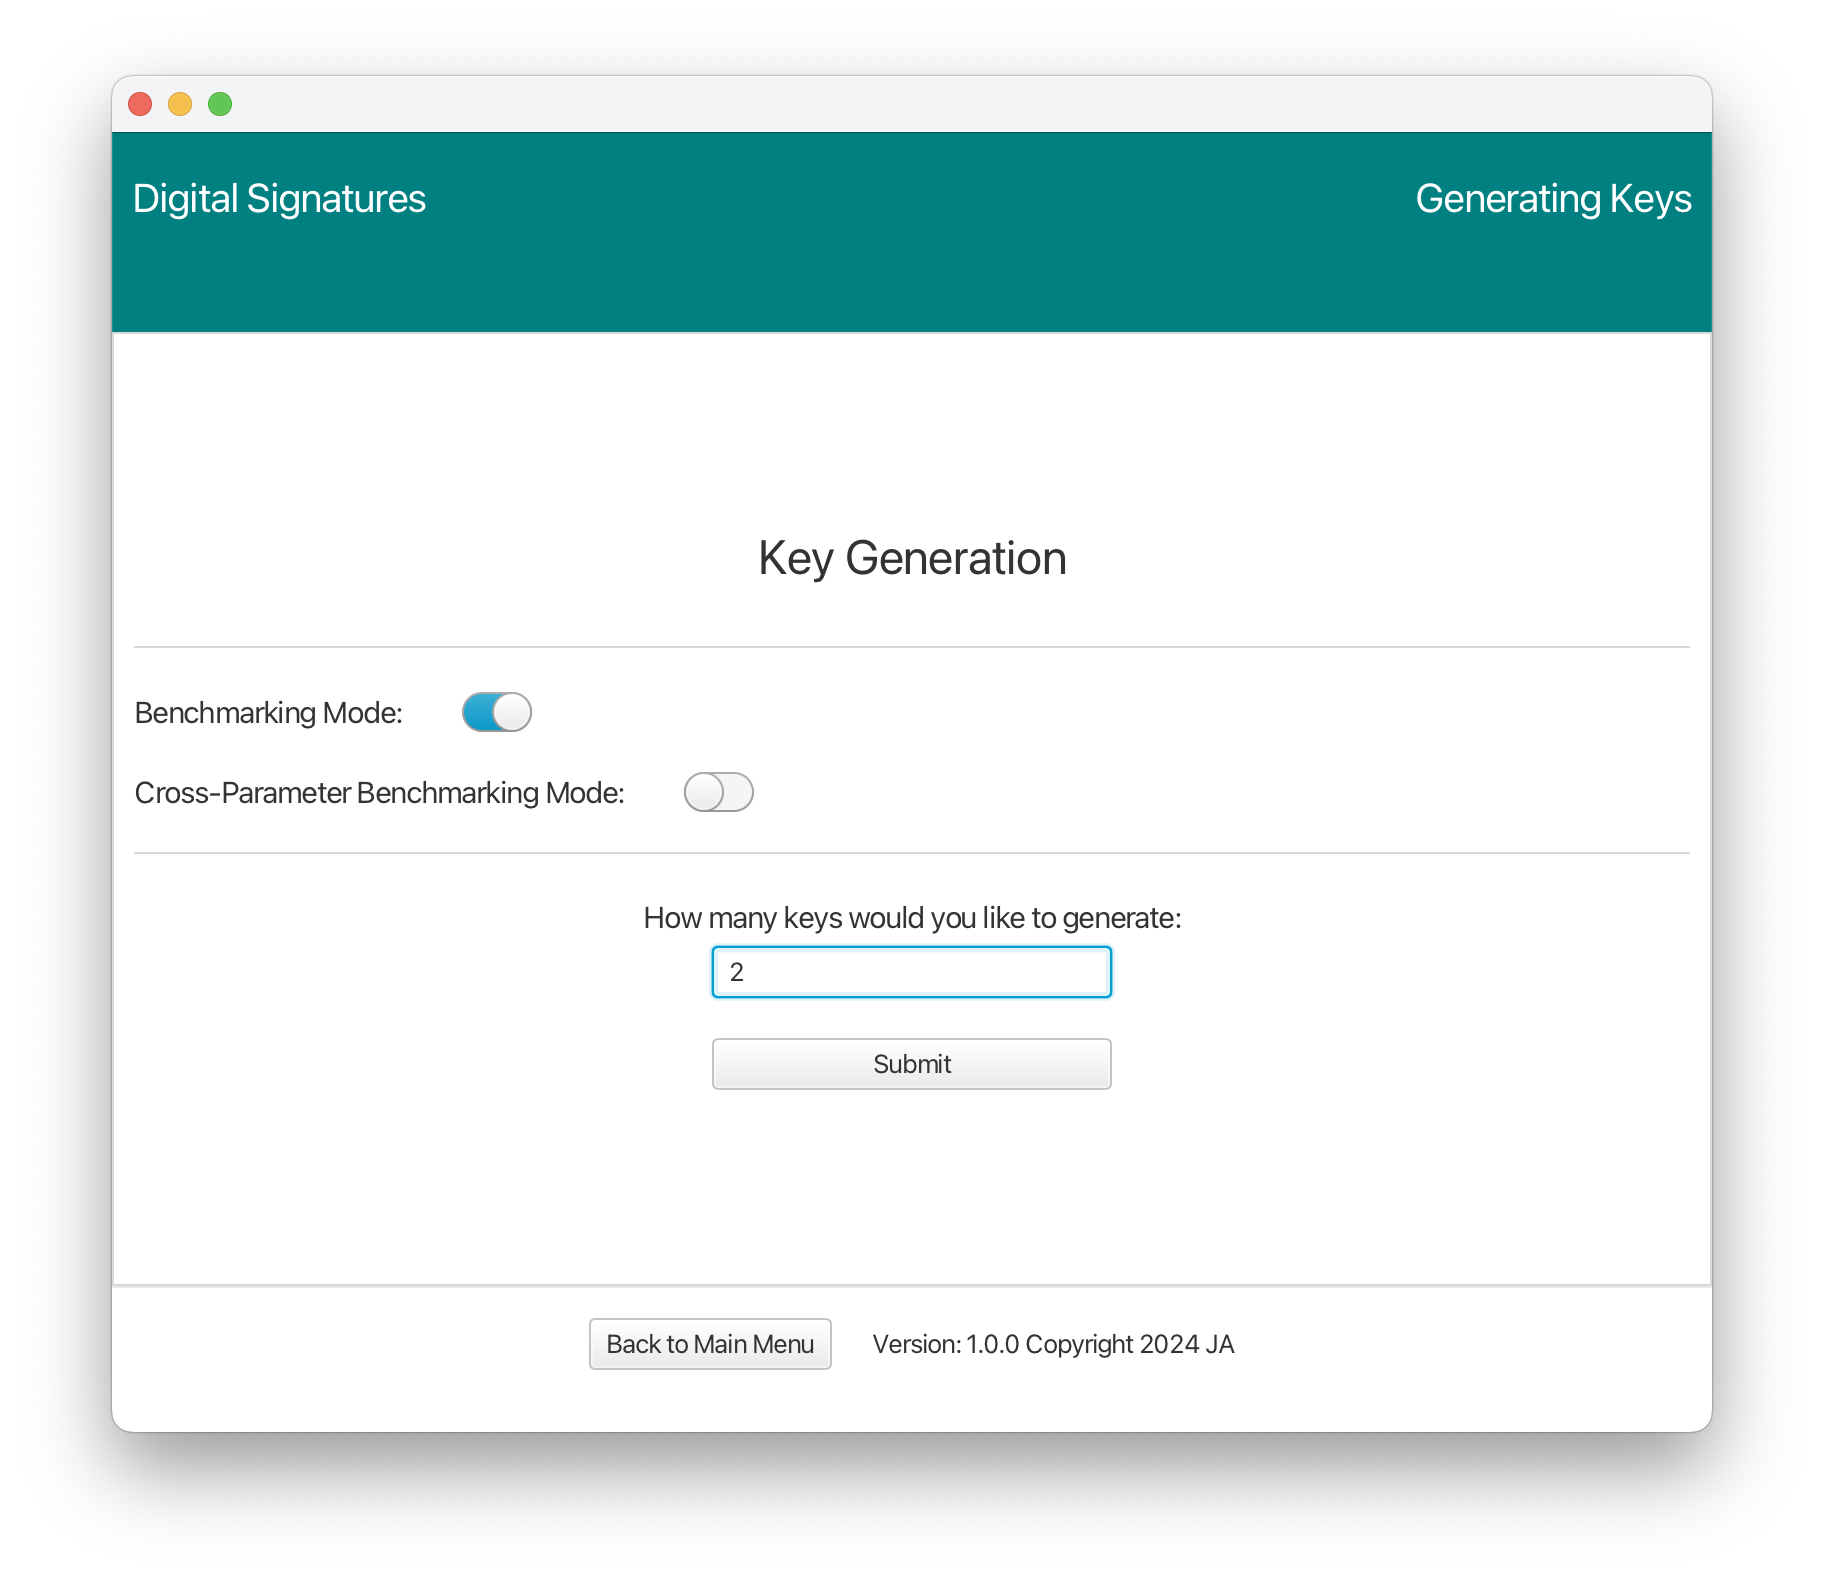
\includegraphics[width=\textwidth]{main_pictures/ui/keyGen/benchmarking/keyGen1.png}} % Adding border here
       \caption{Benchmarking: Key Generation (number of keys)}
        \label{fig:image1}
    \end{minipage}
    \hfill % Add some space between the images
    % Second image in a minipage
    \begin{minipage}{0.495\textwidth}
        \centering
        \fbox{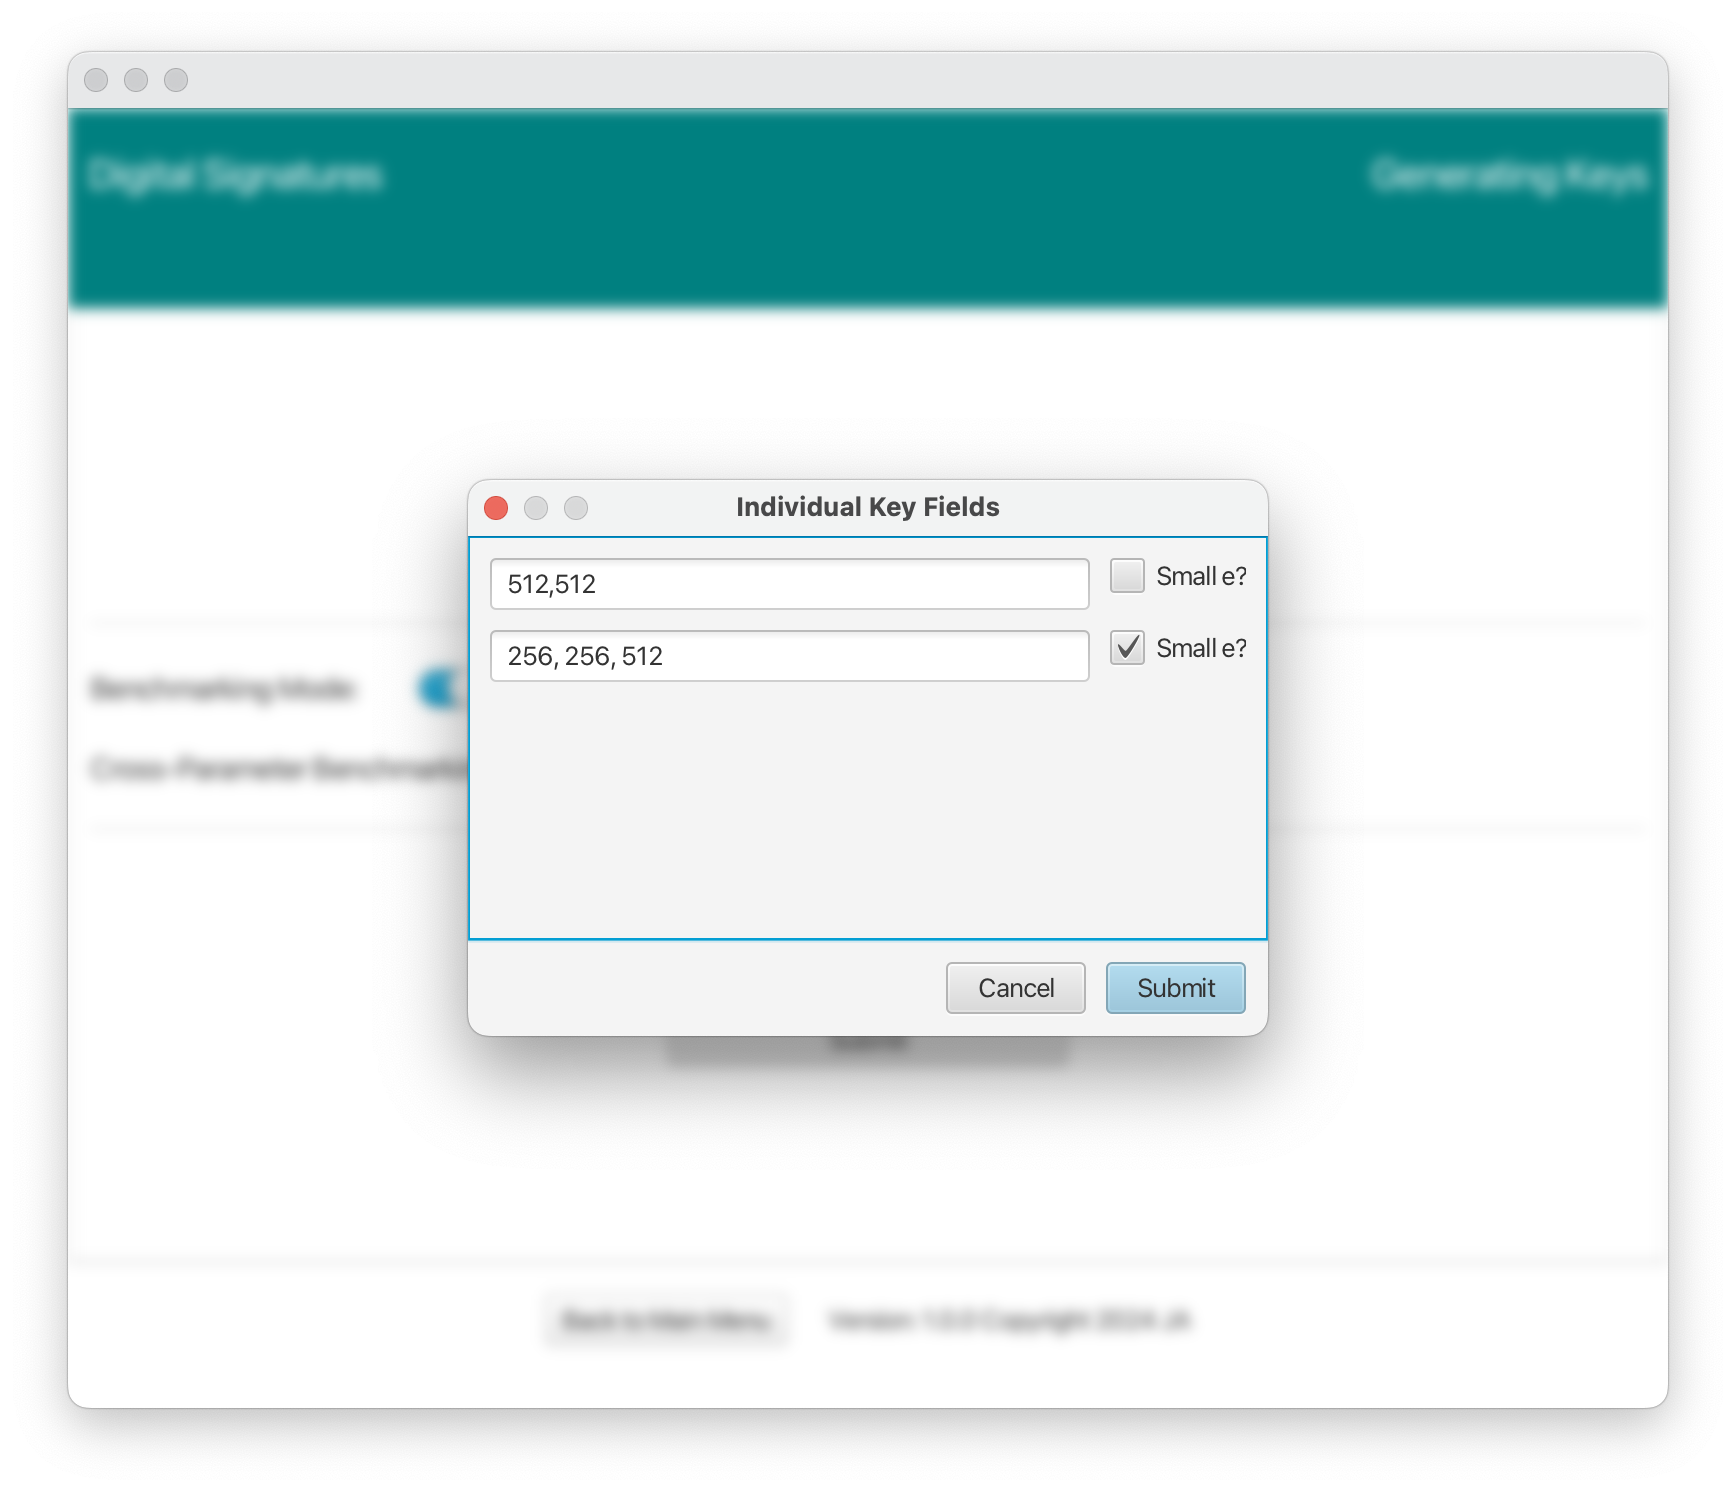
\includegraphics[width=\textwidth]{main_pictures/ui/keyGen/benchmarking/keyGen2.png}} % Adding border here
       \caption{Benchmarking: Key Generation (keys)}
        \label{fig:image2}
    \end{minipage}
    
     \begin{minipage}{0.55\textwidth}
        \centering
        \fbox{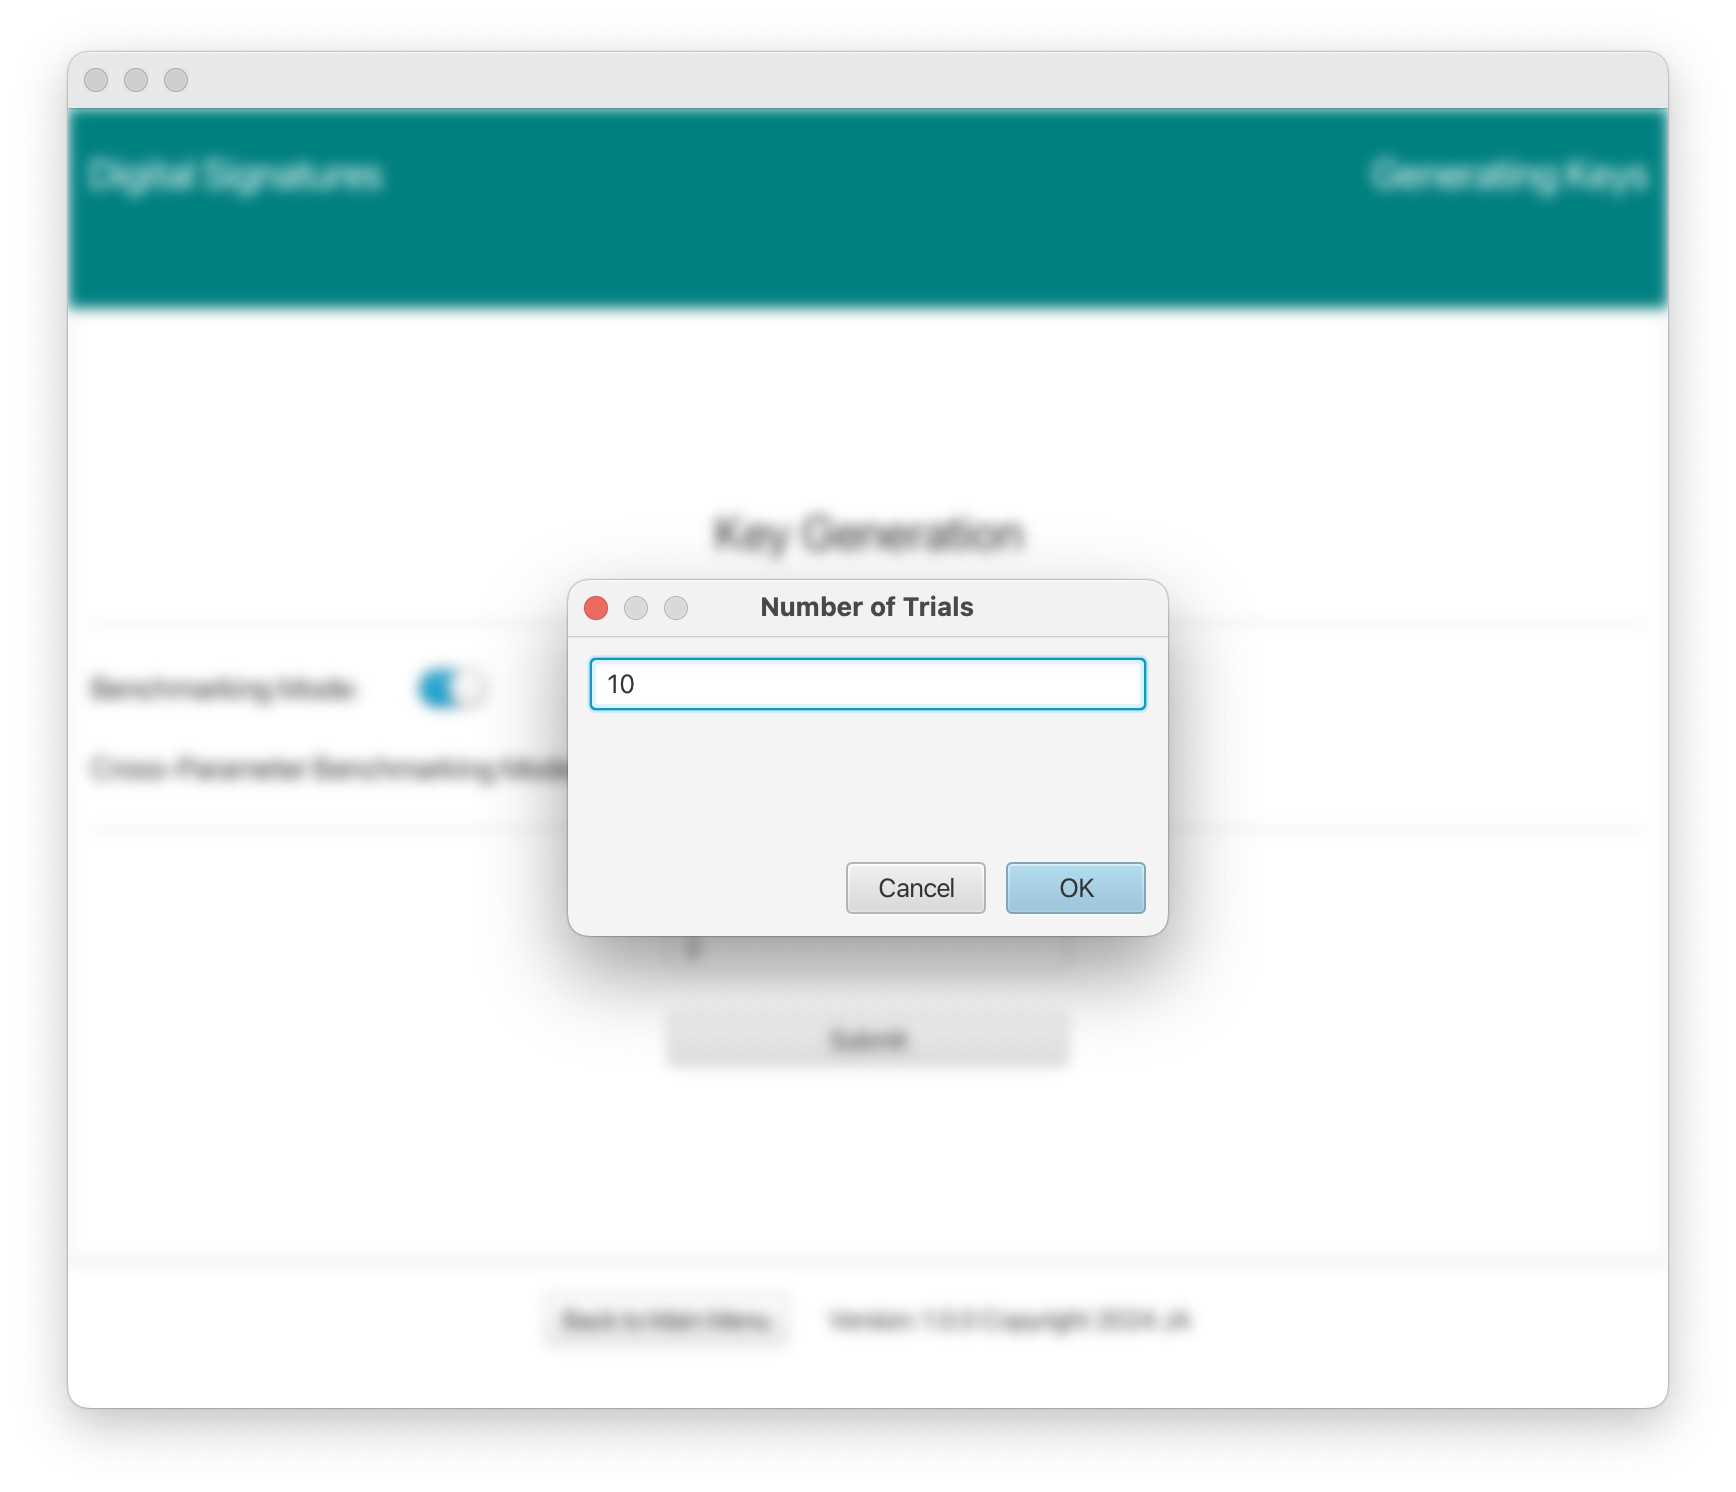
\includegraphics[width=\textwidth]{main_pictures/ui/keyGen/benchmarking/keyGen3.png}} % Adding border here
       \caption{Benchmarking: Key Generation (number of trials)}
        \label{fig:image2}
    \end{minipage}
\end{figure}
The key generation interface for benchmarking is default when selecting key generation on application launch. This interface initially offers a text field to specify the number of individual keys sought to tested.

The application processes the request and then updates the screen with the corresponding of number input pairings displayed vertically down the screen in a dialog box.


Each input corresponding to an individual key configuration consists of a pair of options:
\begin{itemize}
    \item A textfield to input the the configuration of the key
    \item A checkbox labelled small e for specifying whether a small public exponent (less than 1/4 of key size should) be used when generating the key.
\end{itemize}
In the displayed example, the first key configuration is provided as 512, 512 (no small e) and the second as 256, 256, 512 (small e).

Subsequently via an updated dialog, the number of  trials intended for the benchmarking of the key generation process can then be entered. In the current scenario with 10 trials, a benchmarking run would consist of running 10 key generations for each of the selected keys.


Clicking the "OK" button on the number of trials dialog sets the benchmarking process in motion. A progress bar is displayed for a length of time spanning the duration of the task allowing for real-time indication of progress.


\begin{figure}[H]
    \centering
    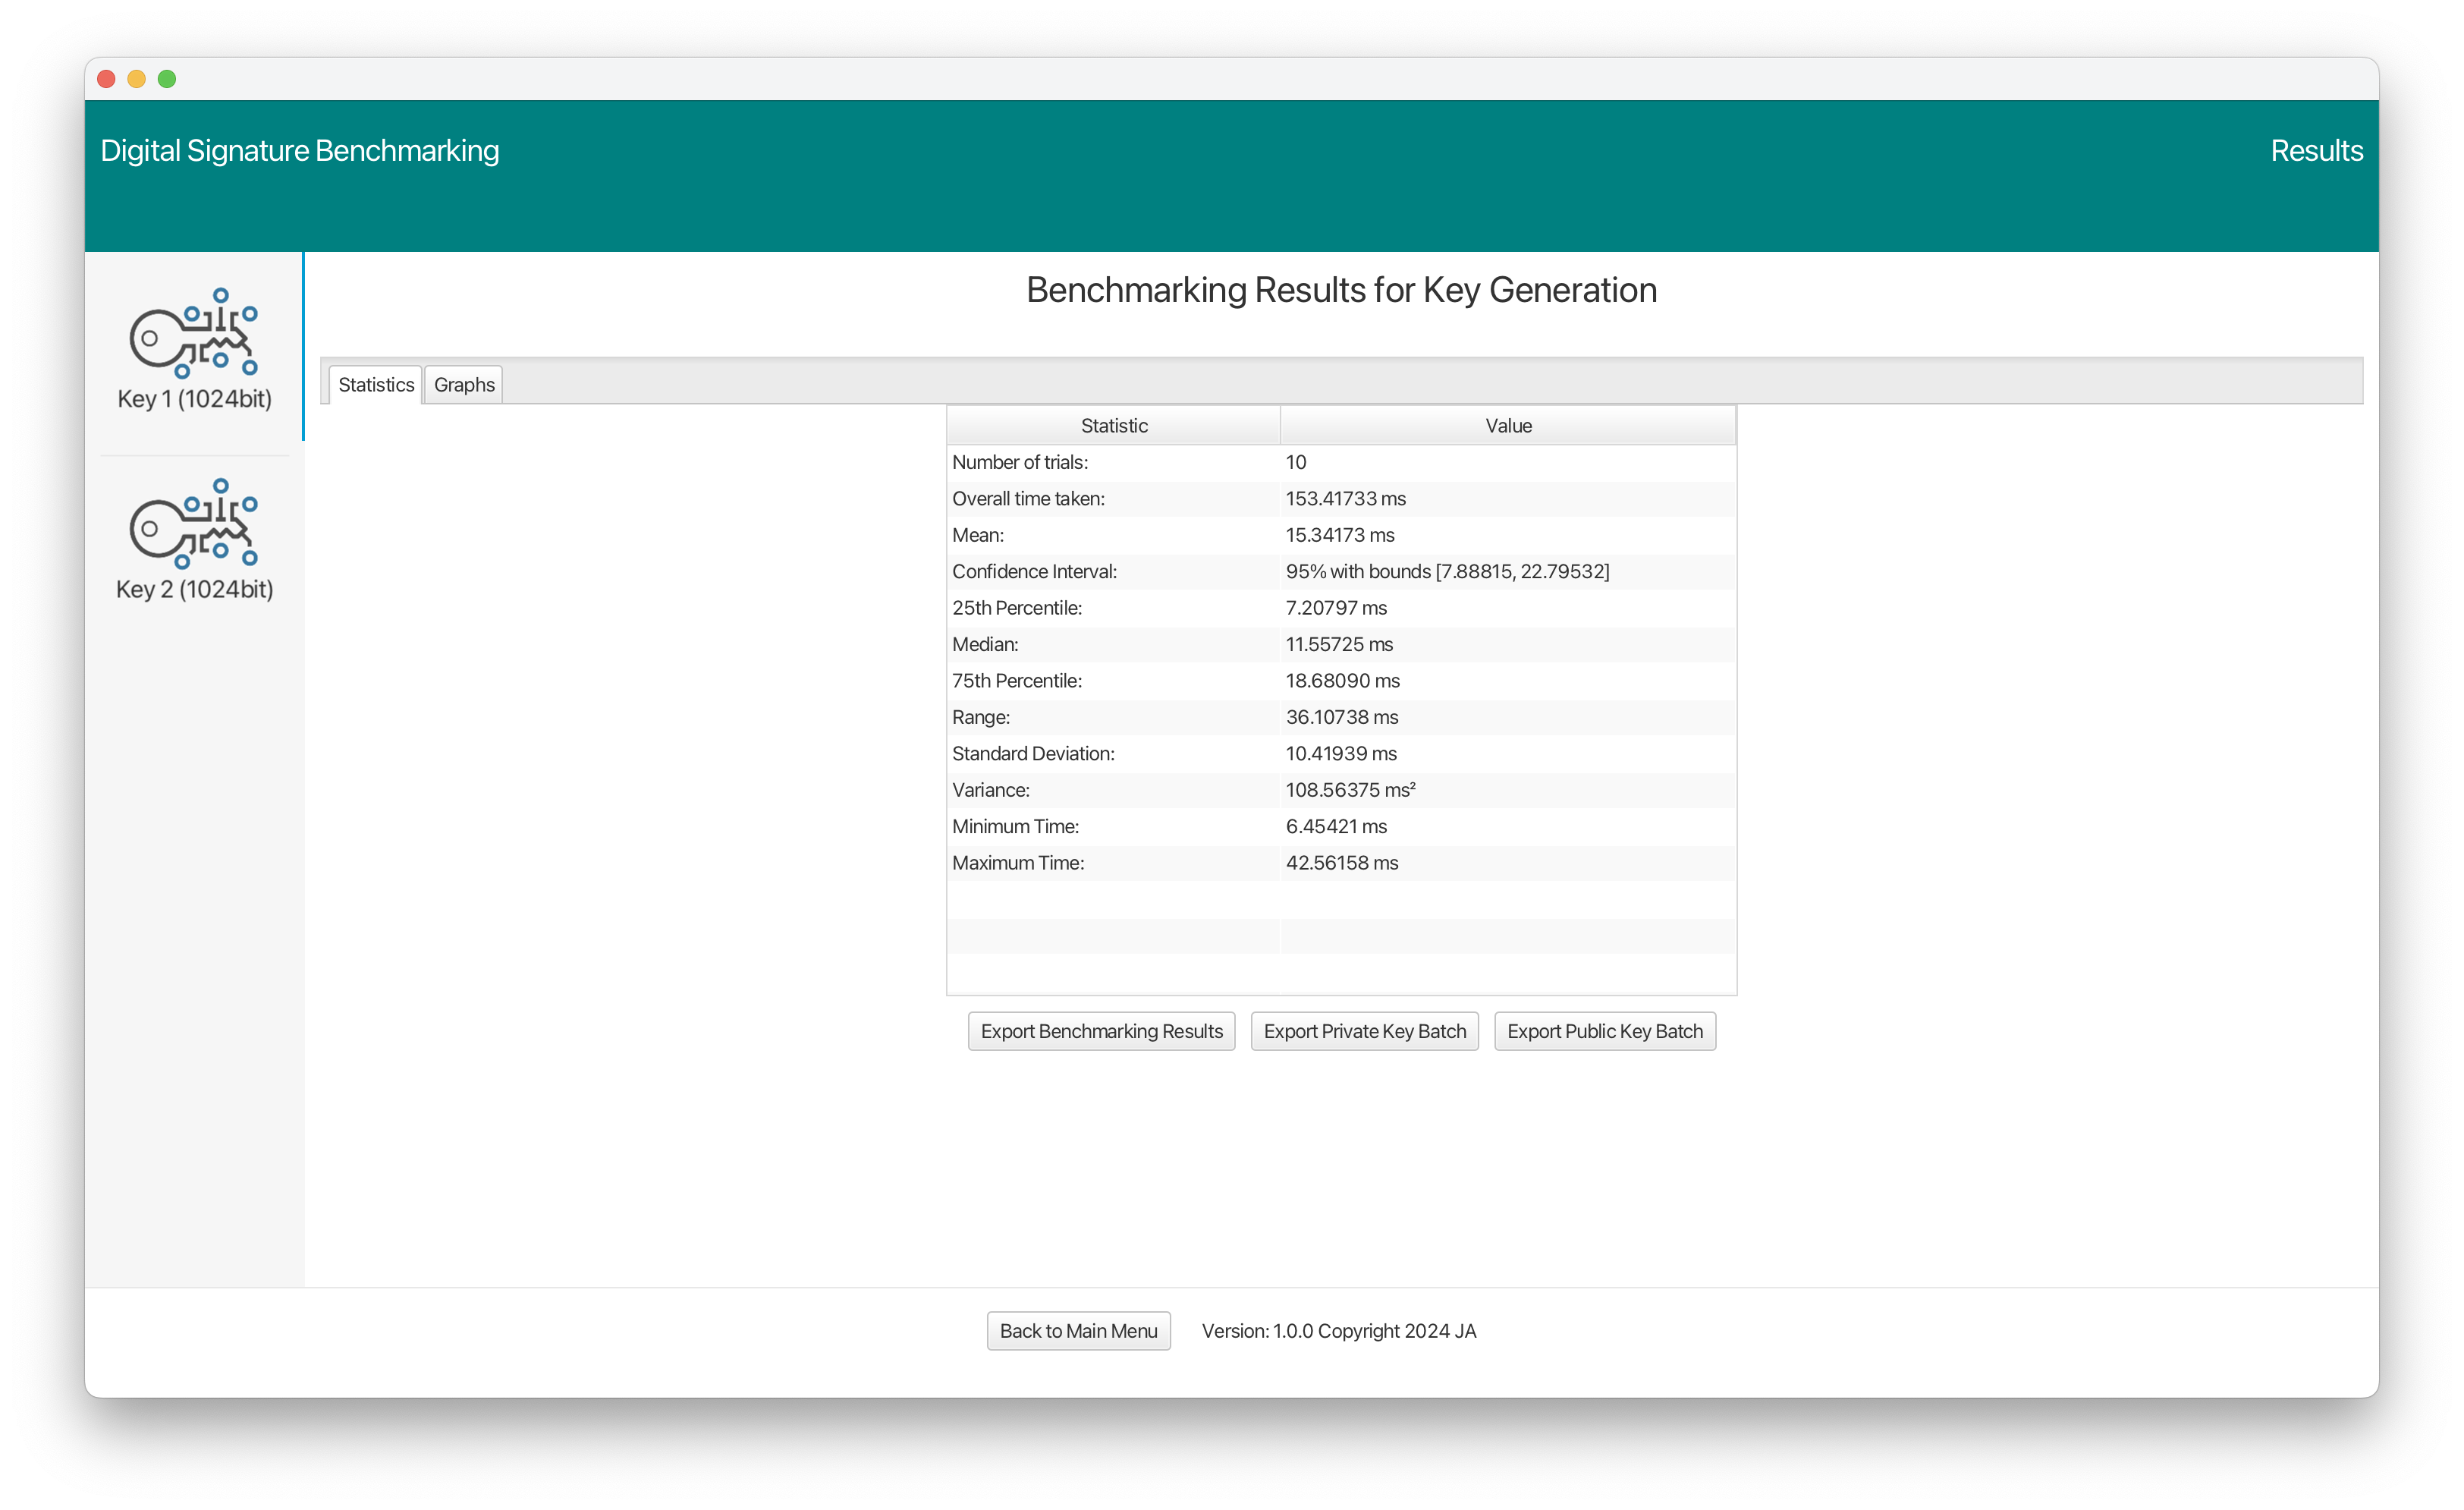
\includegraphics[scale= 0.325]{main_pictures/ui/keyGen/benchmarking/keyGen4.png}
   \caption{Benchmarking: Key Generation (Results Screen)}
\end{figure}

After completing key generation benchmarking, results from benchmarking are displayed. The results screen features a side pane with tabs for each key previously entered. Each tab reveals a results table displaying a statistical metric on each row (mean, range, variance etc) for the key.

Below the results table, the application also provides the functionality to export the benchmarking results and if desired public or private key batches corresponding to a global set of keys matching the key configurations enumerated in a sequence.


\subsection{Signature Generation}


\begin{figure}[H]
    \centering % Center the images
    
    % First image in a minipage
    \begin{minipage}{0.4\textwidth}
        \centering
        \fbox{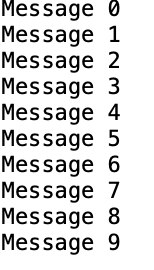
\includegraphics[width=0.4\textwidth]{main_pictures/ui/signing/signing2.png}} % Adding border here
       \caption{Benchmarking: Signature Creation (Test message batch (testMessages.txt))}
        \label{fig:image1}
    \end{minipage}
    \hfill % Add some space between the images
    % Second image in a minipage
    \begin{minipage}{0.58\textwidth}
        \centering
        \fbox{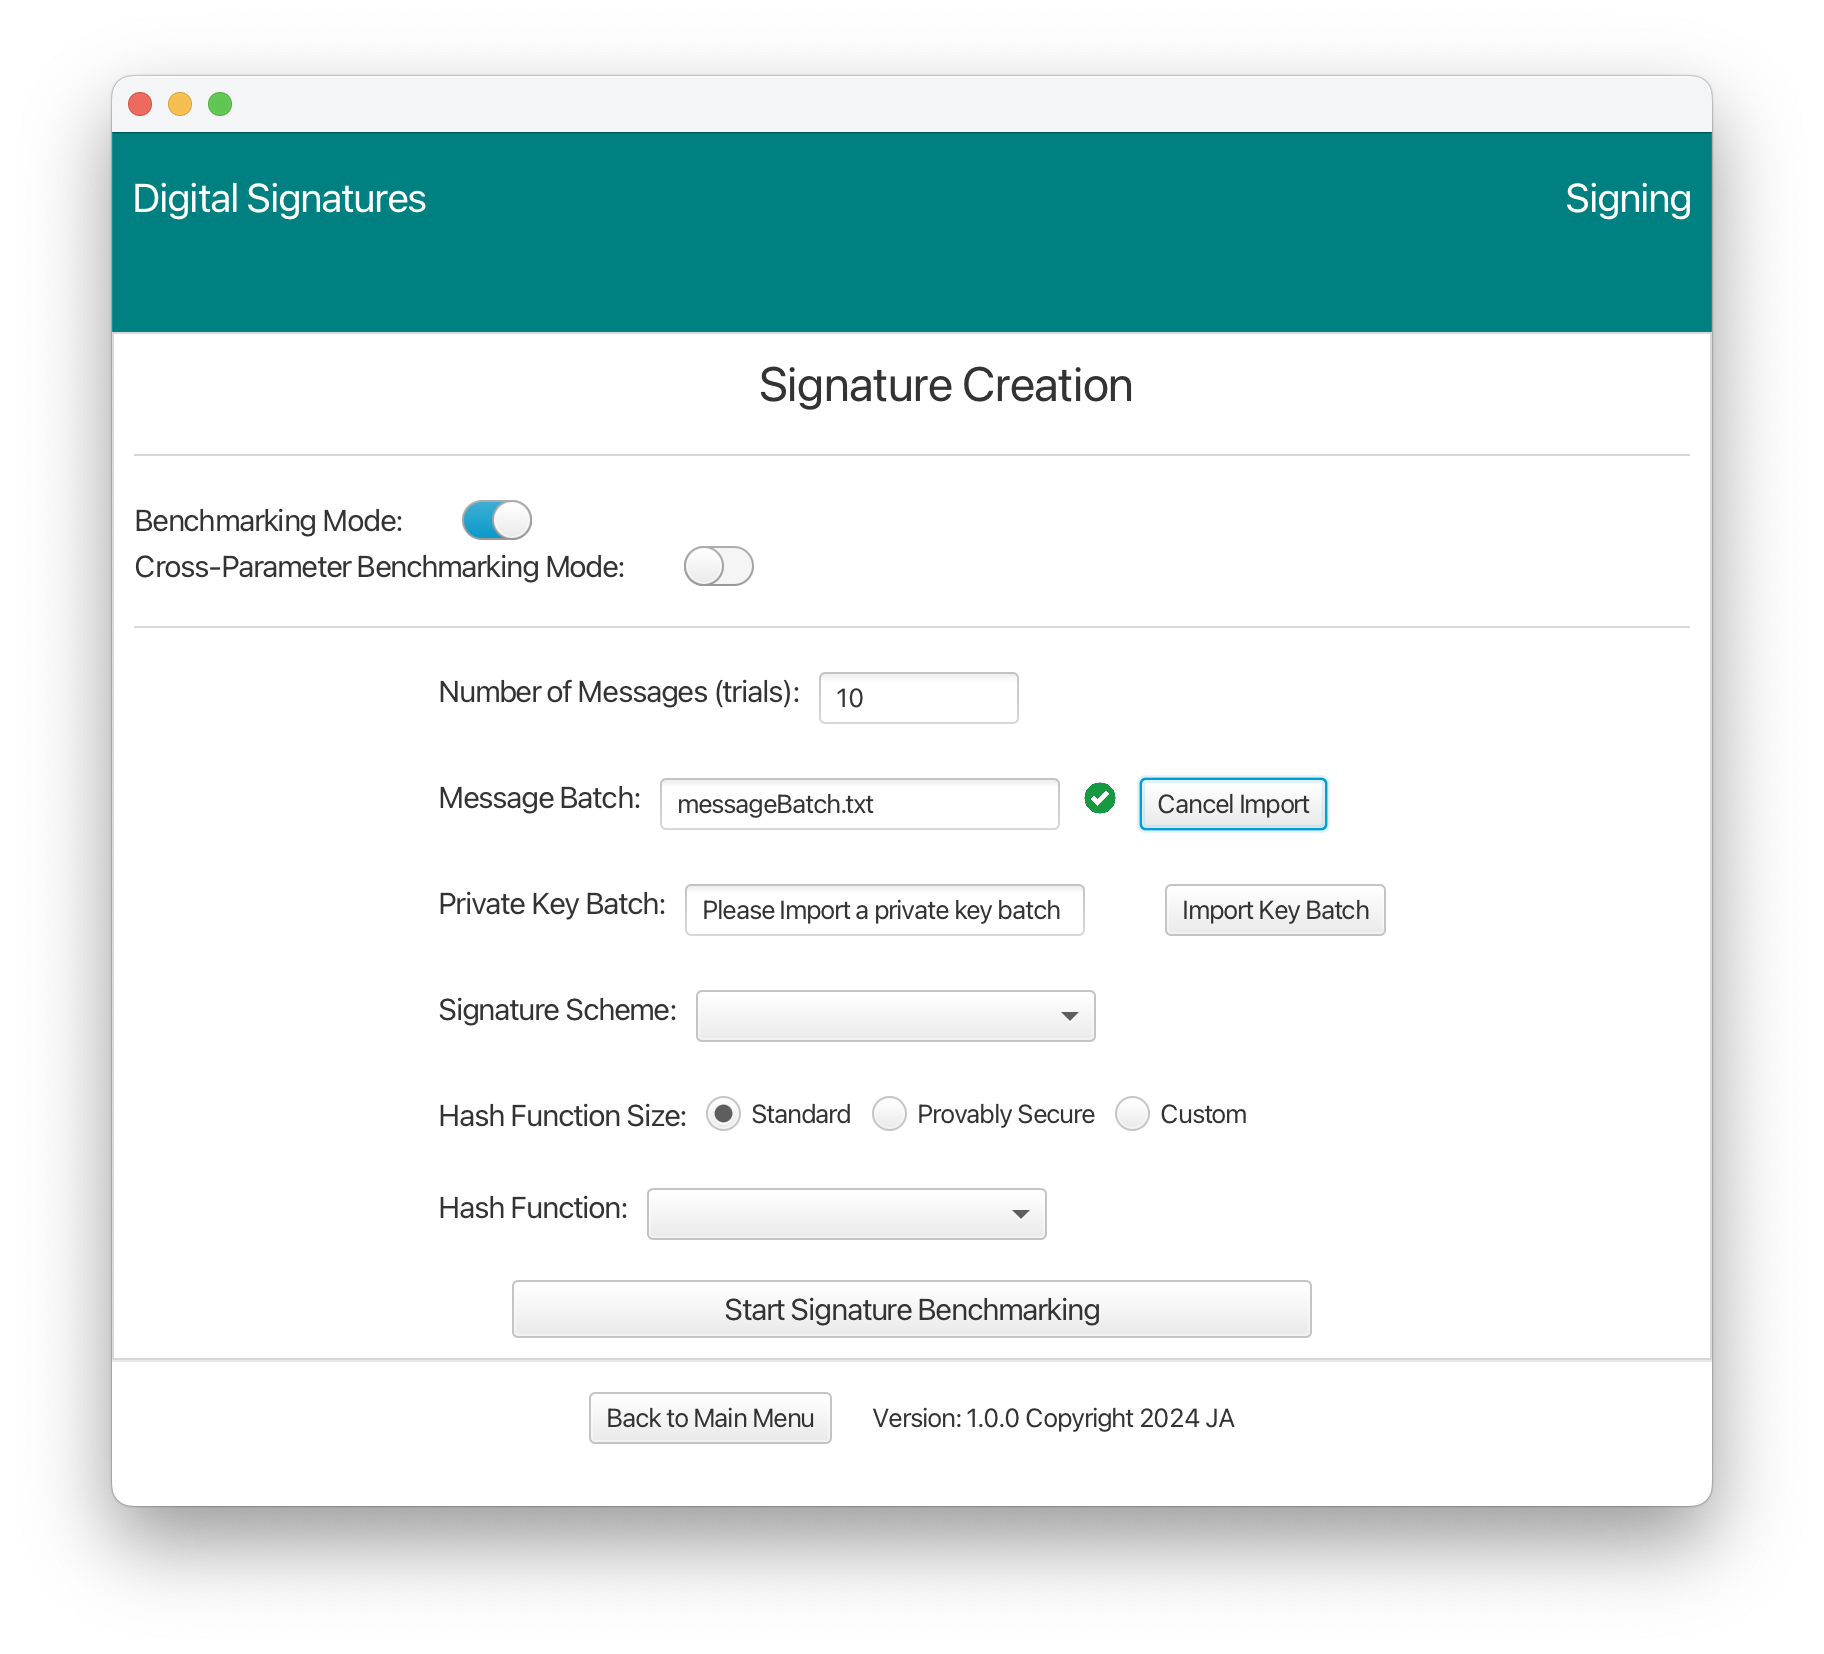
\includegraphics[width=\textwidth]{main_pictures/ui/signing/benchmarking/signing1.png}} % Adding border here
       \caption{Benchmarking: Signature Creation (Imported message batch)}
        \label{fig:image2}
    \end{minipage}
    
\end{figure}

The initial signature generation screen for benchmarking mode is displayed by default when selecting the relevant option from main menu on application launch.
The signature creation screen is first organised with a pair of fields related to the importing of a message batch. There are specific requirements for the import of the message batch. 

The application expects the message batch as a non interrupted and new line separated sequence of messages and the number of lines must match the number entered in the adjacently above field. Otherwise import of a message batch is prevented. 

On successful validation, the screen is updated with a checkmark indicator that provides visual confirmation that the message batch was successfully imported. Below this is the private key batch import section, which also confirms successful key loading with a checkmark.

The interface also includes a dropdown menu labeled signature scheme giving users the option to select the desired signature scheme  to be applied. 

\begin{figure}[H]
    \centering % Center the images
    
    % First image in a minipage
    \begin{minipage}{0.49\textwidth}
        \centering
        \fbox{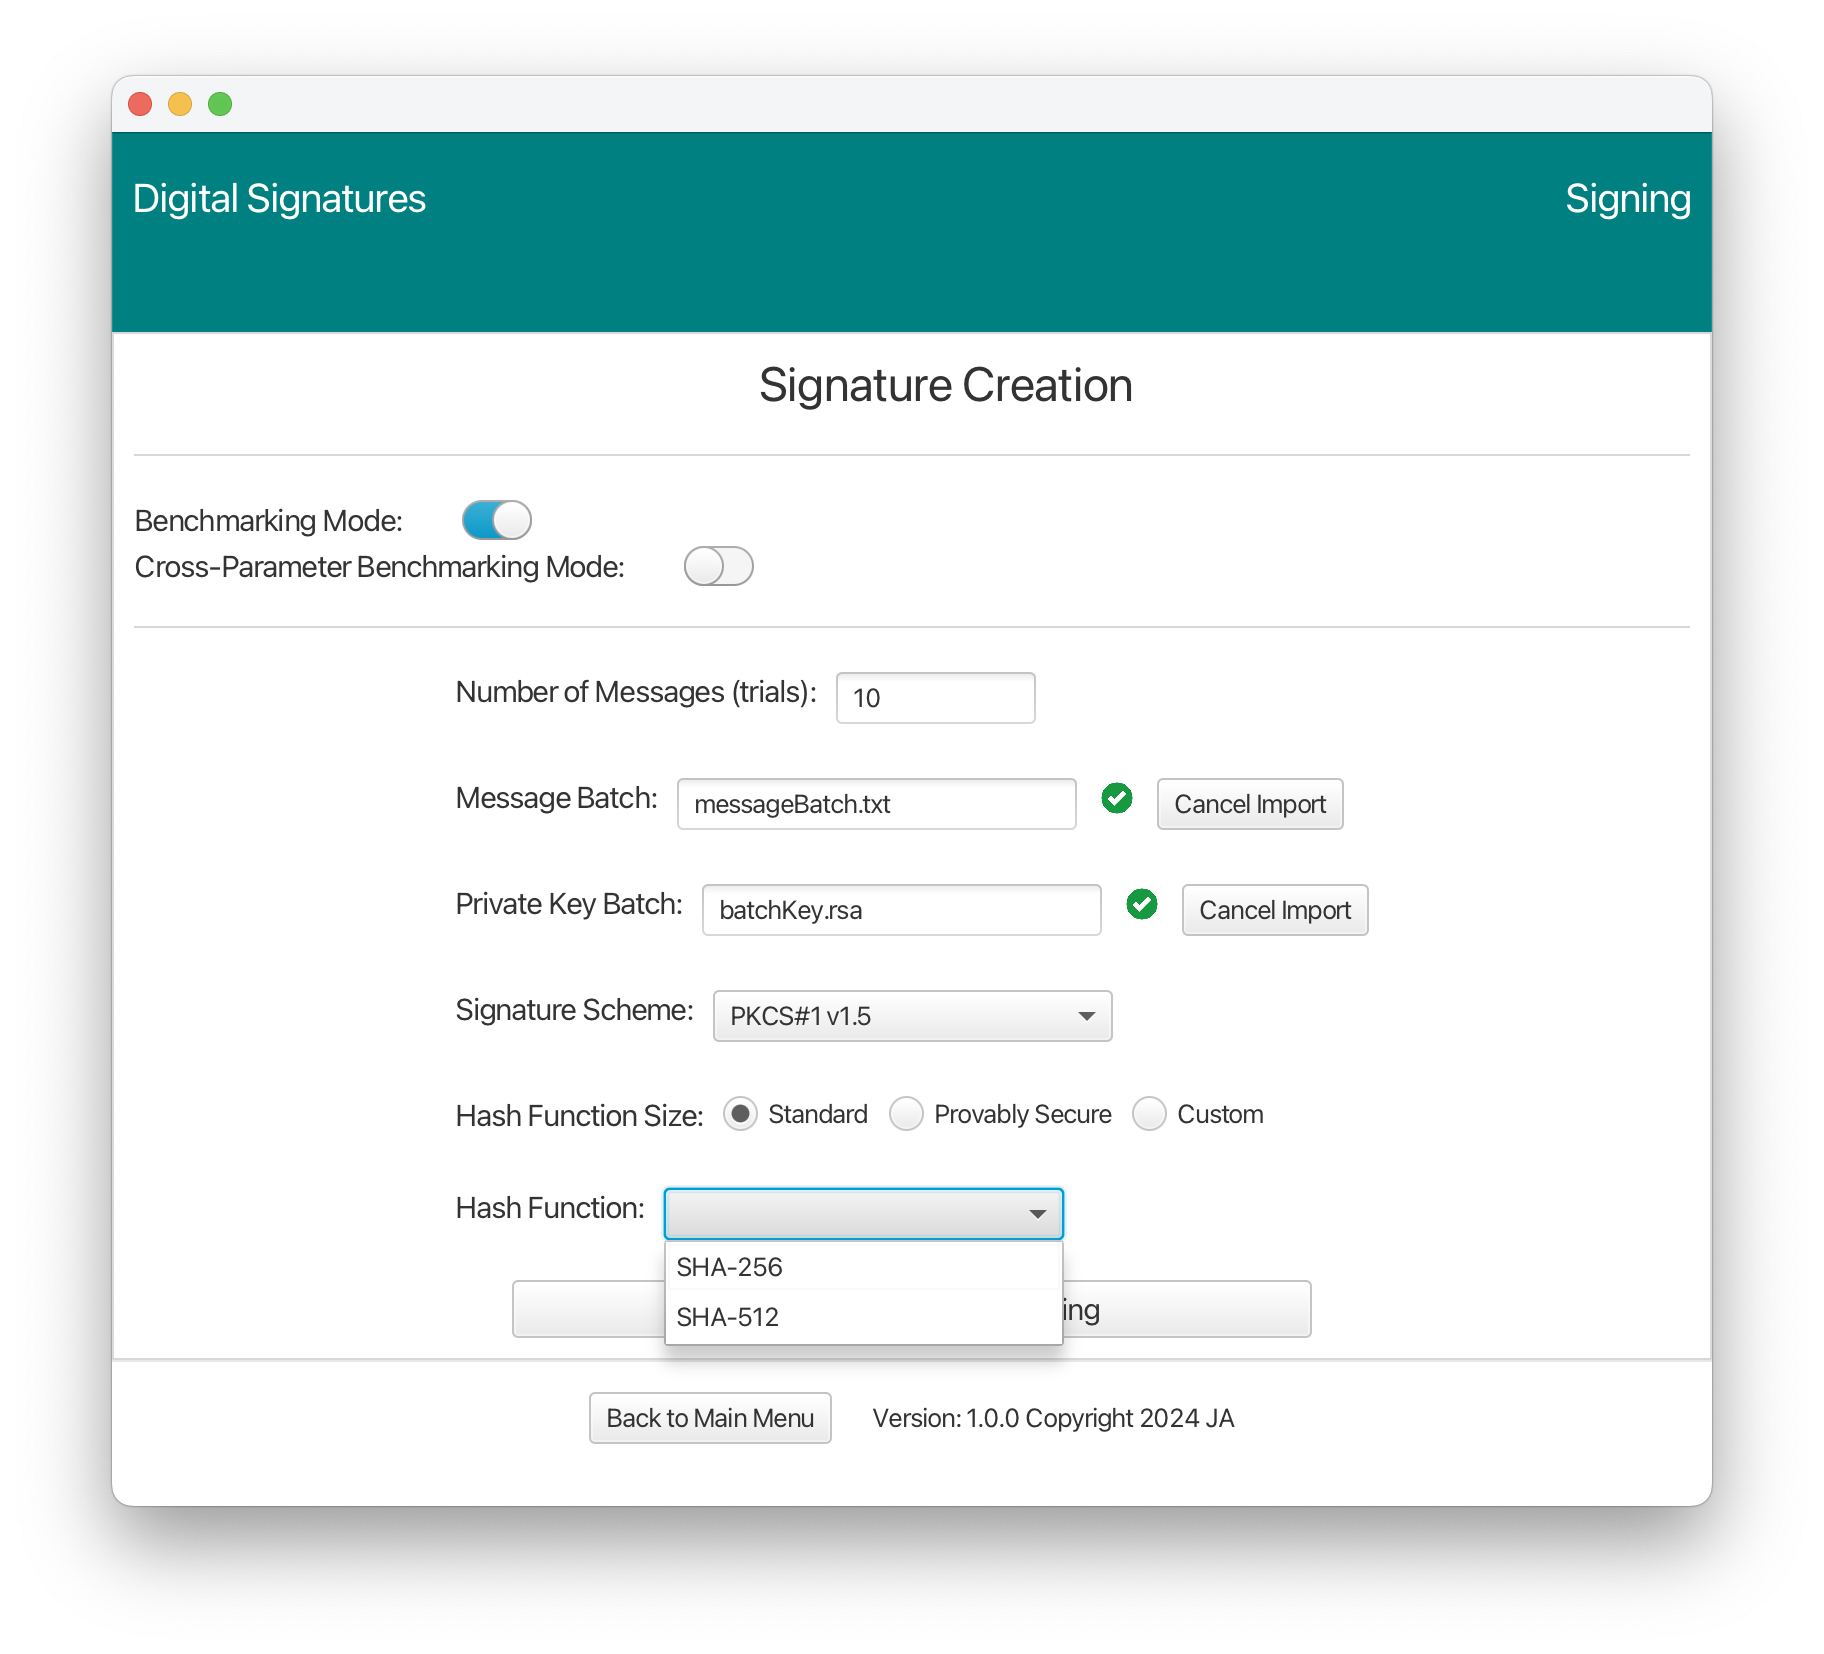
\includegraphics[width=\textwidth]{main_pictures/ui/signing/benchmarking/signing2.png}} % Adding border here
       \caption{Benchmarking: Signature Creation (Hash Function Choice for Standard Hash size)}
        \label{fig:image1}
    \end{minipage}
    \hfill % Add some space between the images
    % Second image in a minipage
    \begin{minipage}{0.49\textwidth}
        \centering
        \fbox{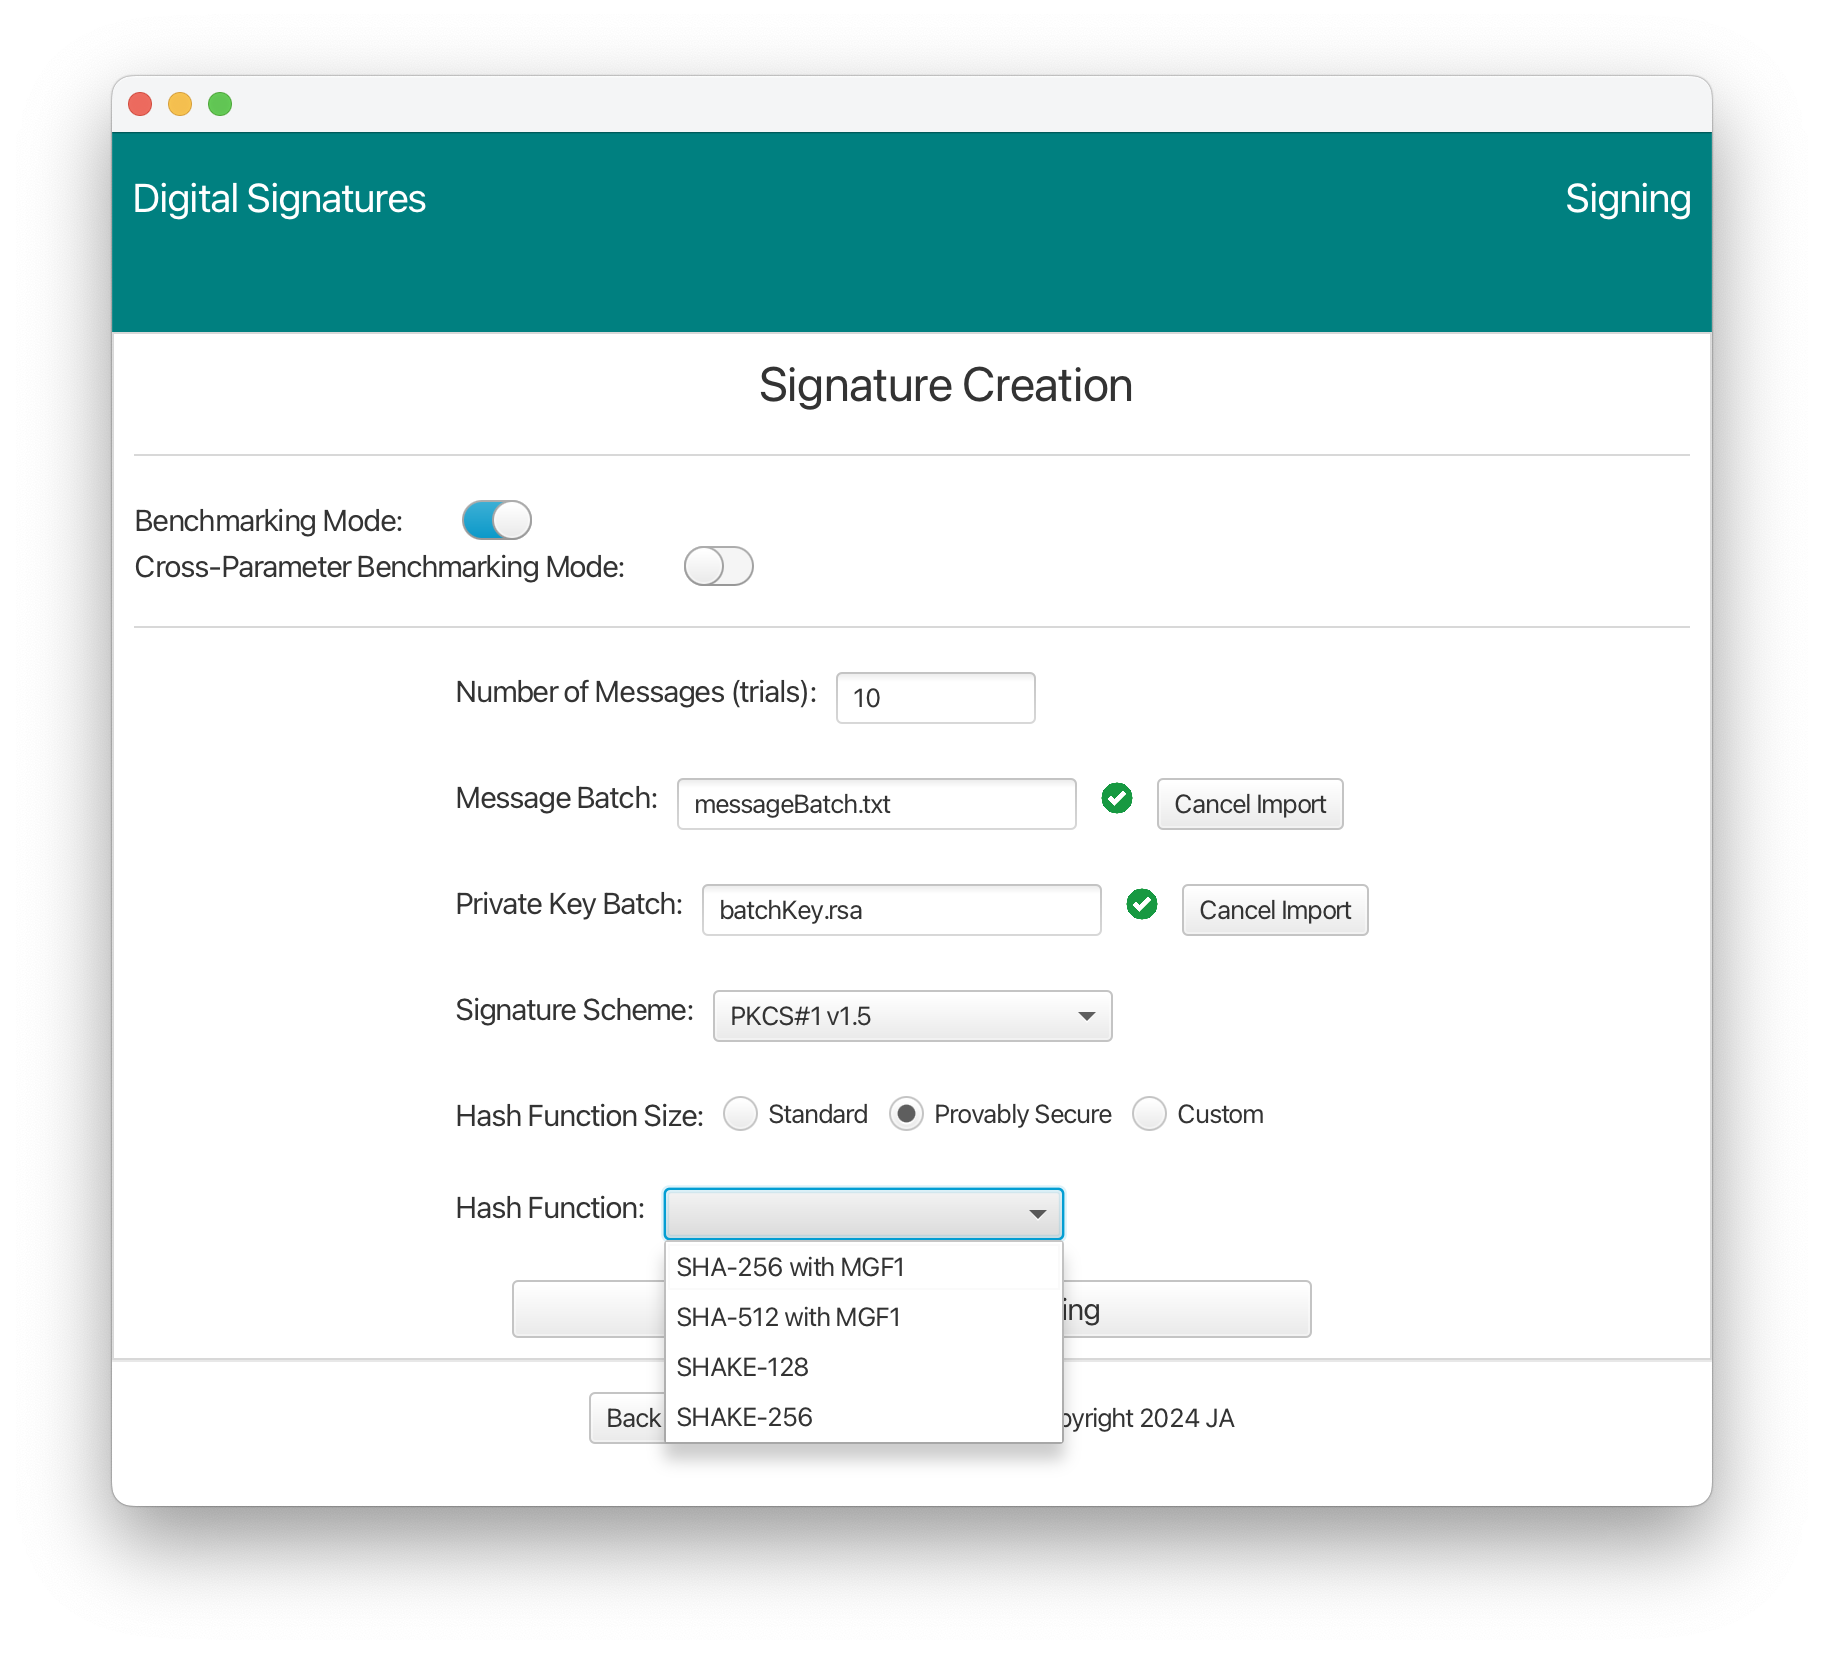
\includegraphics[width=\textwidth]{main_pictures/ui/signing/benchmarking/signing3.png}} % Adding border here
       \caption{Benchmarking: Signature Creation (Hash Function Choice for Provably Secure Hash size)}
        \label{fig:image2}
    \end{minipage}
\end{figure}
\begin{figure}[H]
    \centering % Center the images
    
    % First image in a minipage
    \begin{minipage}{0.49\textwidth}
        \centering
        \fbox{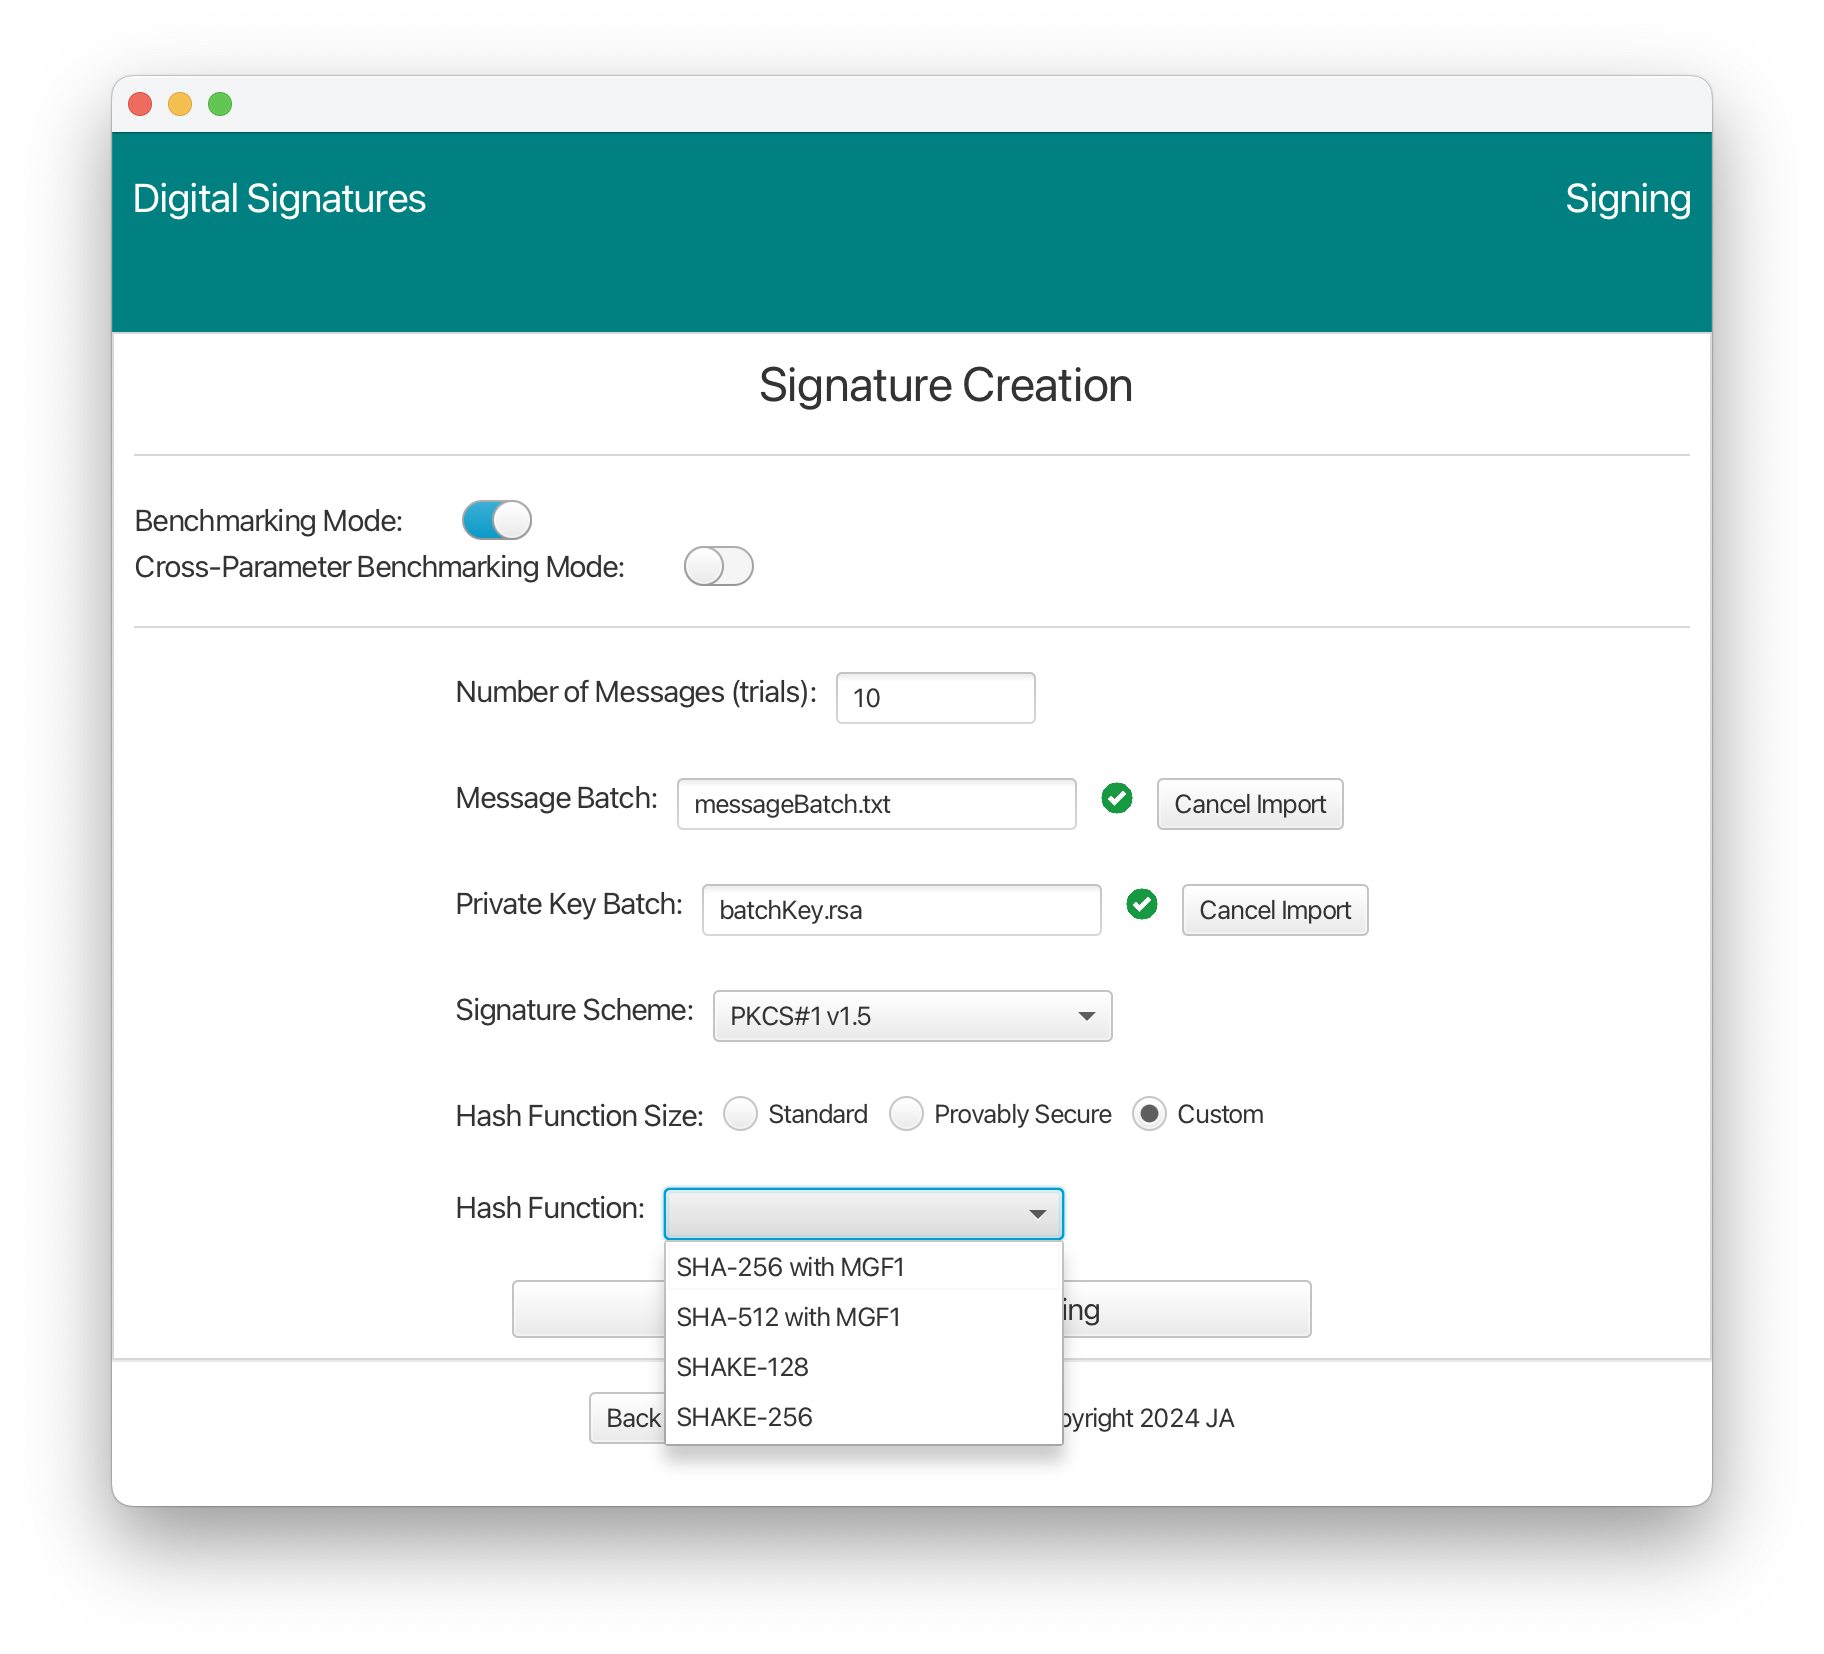
\includegraphics[width=\textwidth]{main_pictures/ui/signing/benchmarking/signing4.png}} % Adding border here
       \caption{Benchmarking: Signature Creation (Hash Function Choice for Custom Hash size)}
        \label{fig:image1}
    \end{minipage}
    \hfill % Add some space between the images
    % Second image in a minipage
    \begin{minipage}{0.49\textwidth}
        \centering
        \fbox{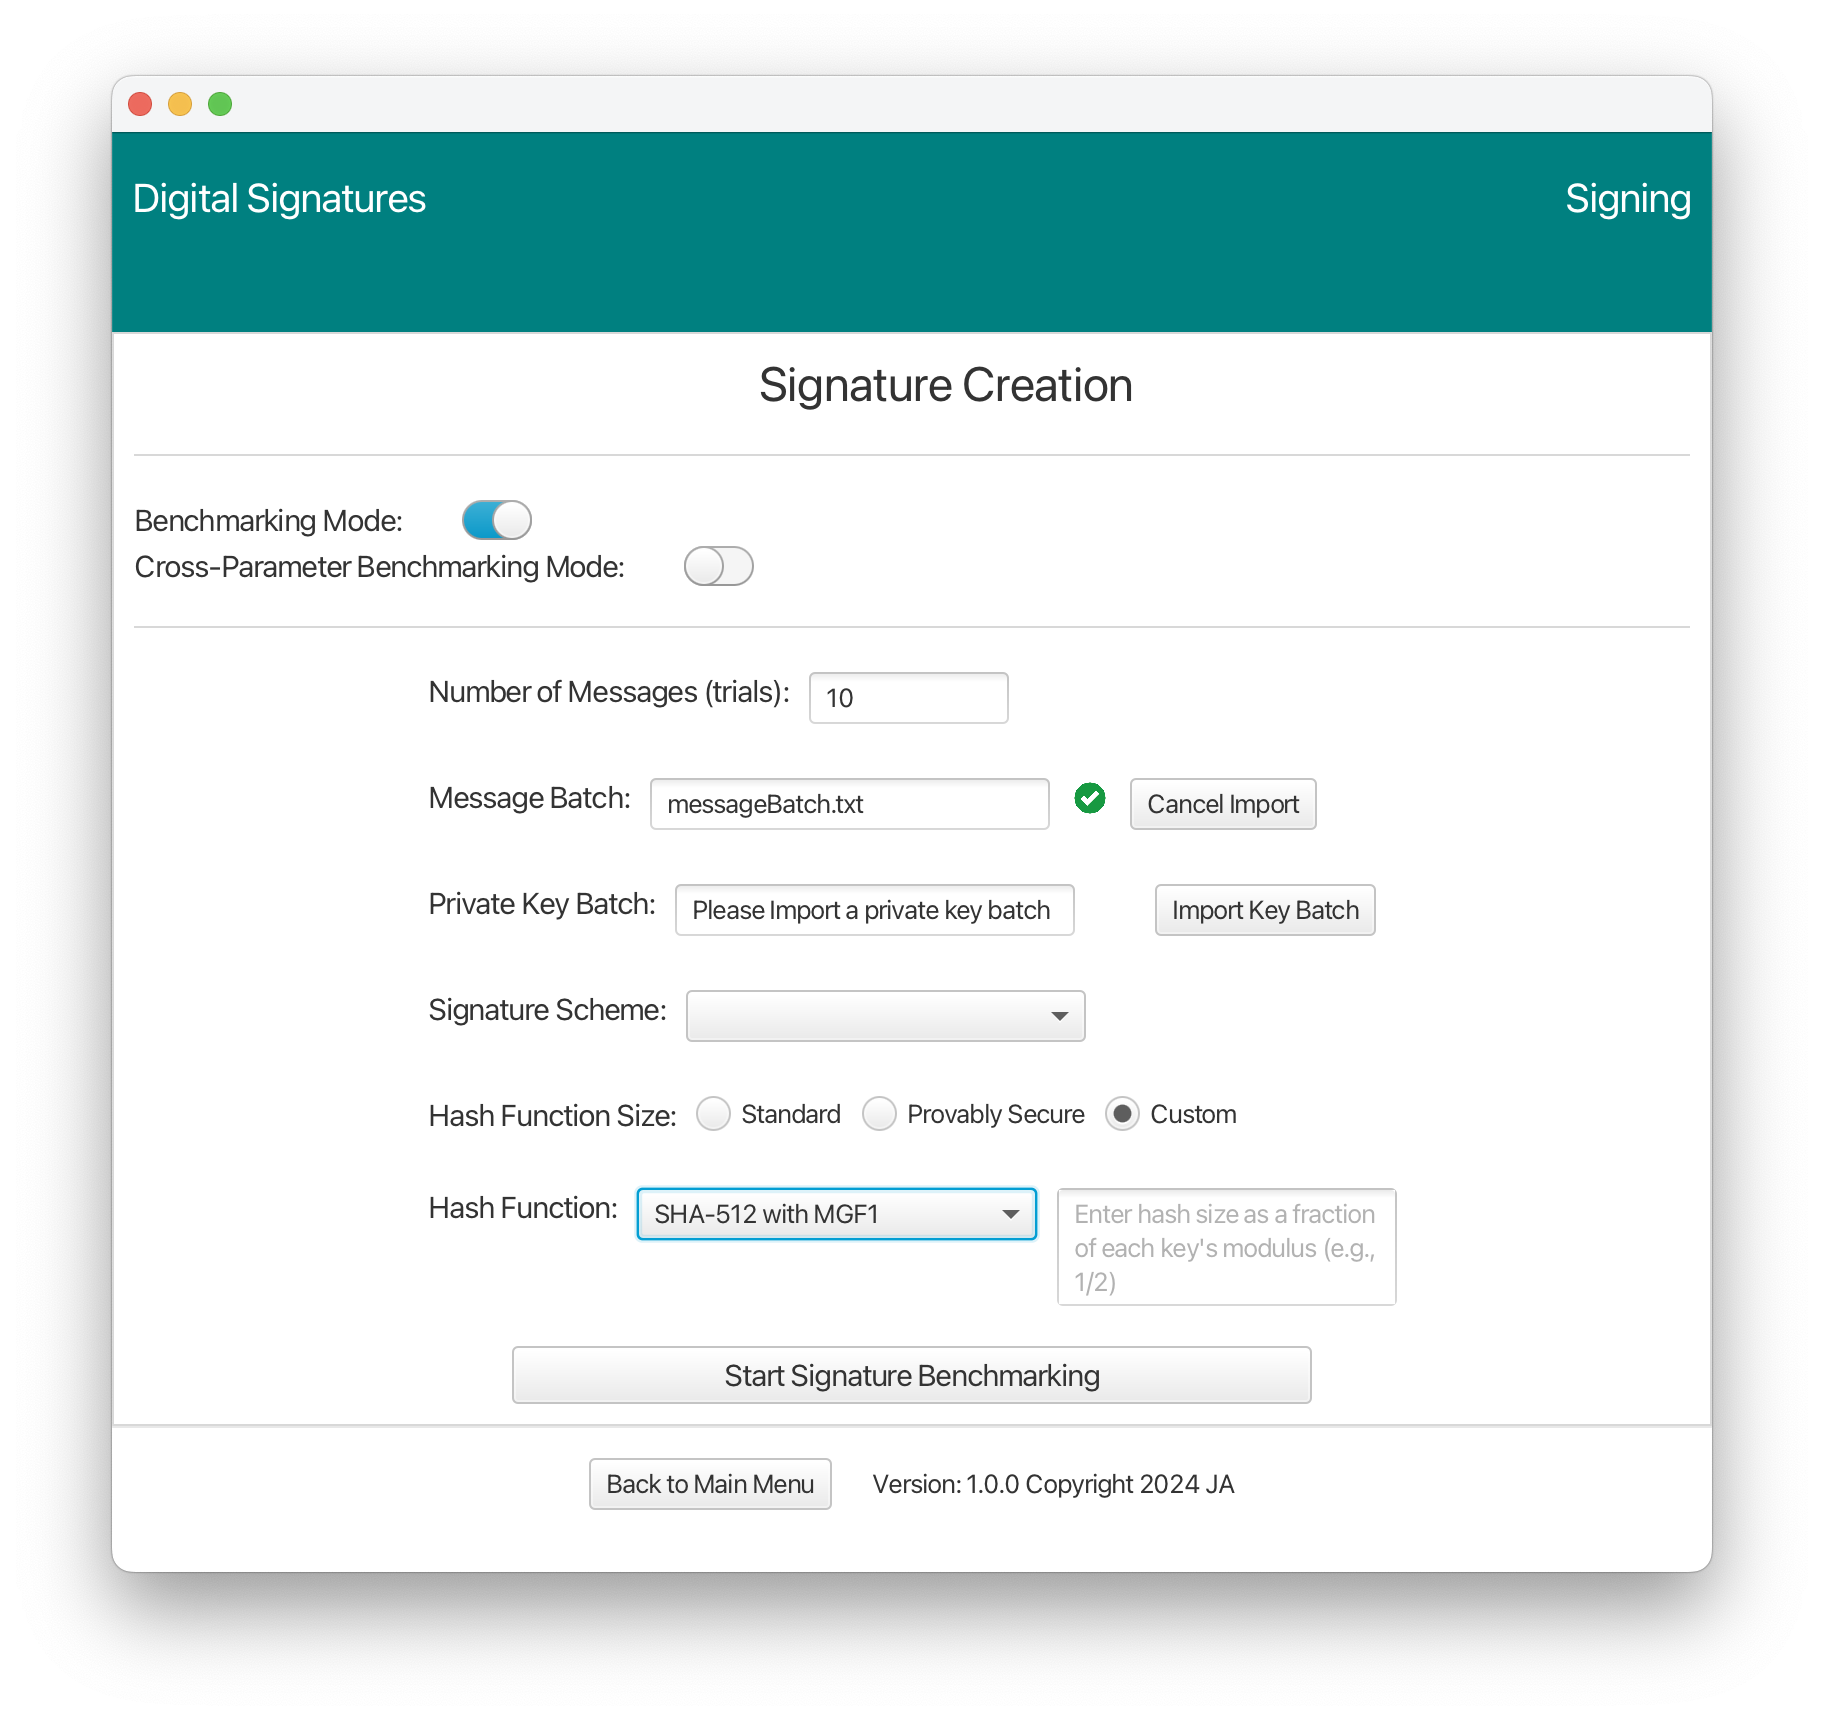
\includegraphics[width=\textwidth]{main_pictures/ui/signing/benchmarking/signing5.png}} % Adding border here
       \caption{Benchmarking: Signature Creation (Input of Custom Hash size)}
        \label{fig:image2}
    \end{minipage}
\end{figure}

The system presents the hash function selection as a decision point:
\begin{itemize}
    \item \textbf{Provably Secure Parameters}: If the option for instantiation with provably secure parameters is selected, the system displays only the variable length hash functions. After the user selects one, the system sets the hash function output size to half the modulus length for each key.
    \item \textbf{Provably Secure Hash Size}: If the user opts for a provably secure hash size, the system again displays only variable length hash functions. Upon selection, the output size is configured to half of the modulus length, aligning with provable security standards.
    \item \textbf{Custom Hash Size}: When a custom hash size is chosen, the user is presented with variable length hash functions. The system then prompts the user to input a custom hash size as a fraction, which it uses to determine the hash function output size in relation to the modulus length of each key.
    \item \textbf{Standard Hash Size}: If the standard hash size is preferred, the system limits the display to fixed length hash functions, from which the user can select.
\end{itemize}


Clicking "Start Signature Benchmarking" button initiates the execution the benchmarking task. This involves the creation of a batch of signatures for the message batch using the designated signature scheme and hash function for every key provided in the private key batch. A progress bar indicates progress in real time.


\textbf{Benchmarking: Signature Generation Results Screen}

\begin{figure}[H]
    \centering
    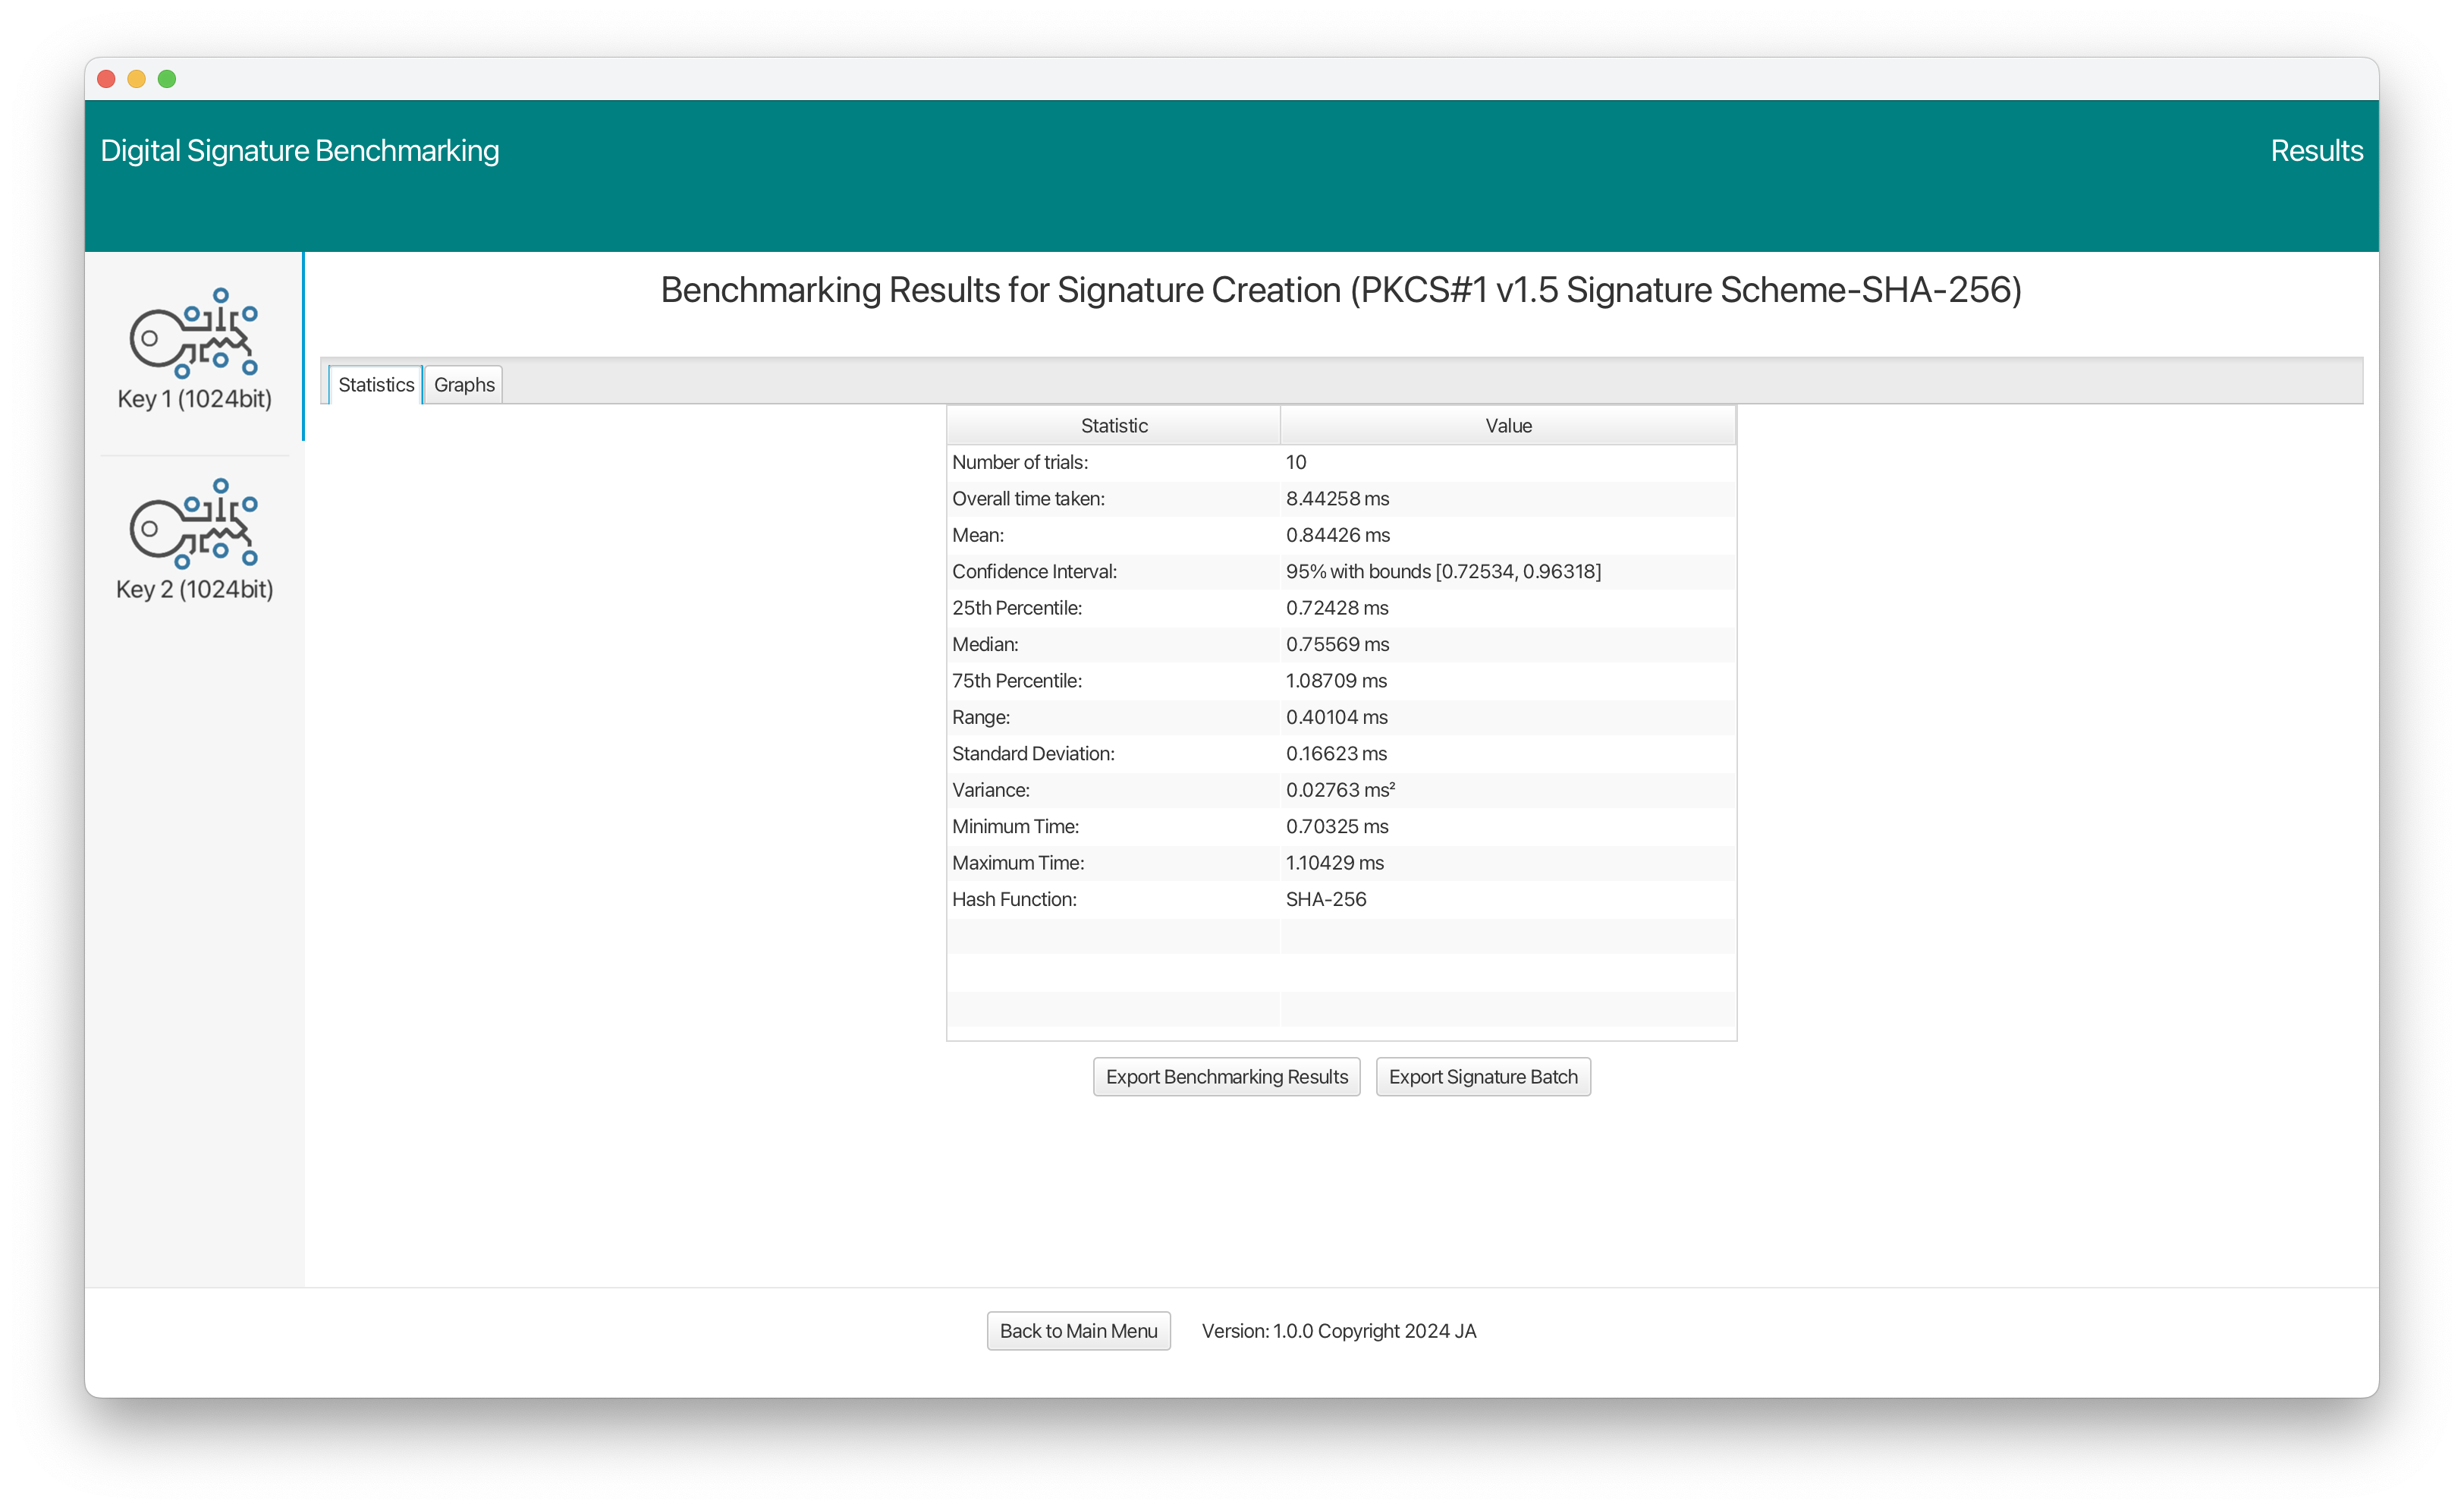
\includegraphics[scale= 0.325]{main_pictures/ui/signing/benchmarking/signing6.png}
   \caption{Benchmarking: Signature Generation (Results Screen)}
\end{figure}

After completing signature generation benchmarking, results from benchmarking are displayed. The results screen features a side pane with tabs for each key previously entered. Each tab reveals a results table displaying a statistical metric on each row (mean, range, variance etc) for the key, with the final row indicating the hash function that was selected.


Below the table, options are available to export benchmarking results and signature batches for each key size. The exported signature batch aligns with the key configurations and selected hash function, covering all keys in a single file.

\newpage
\textbf{Benchmarking: Signature Generation Results Screen Graphs}

\begin{figure}[H]
    \centering % Center the images
    
    % First image in a minipage
    \begin{minipage}{0.7\textwidth}
        \centering
        \fbox{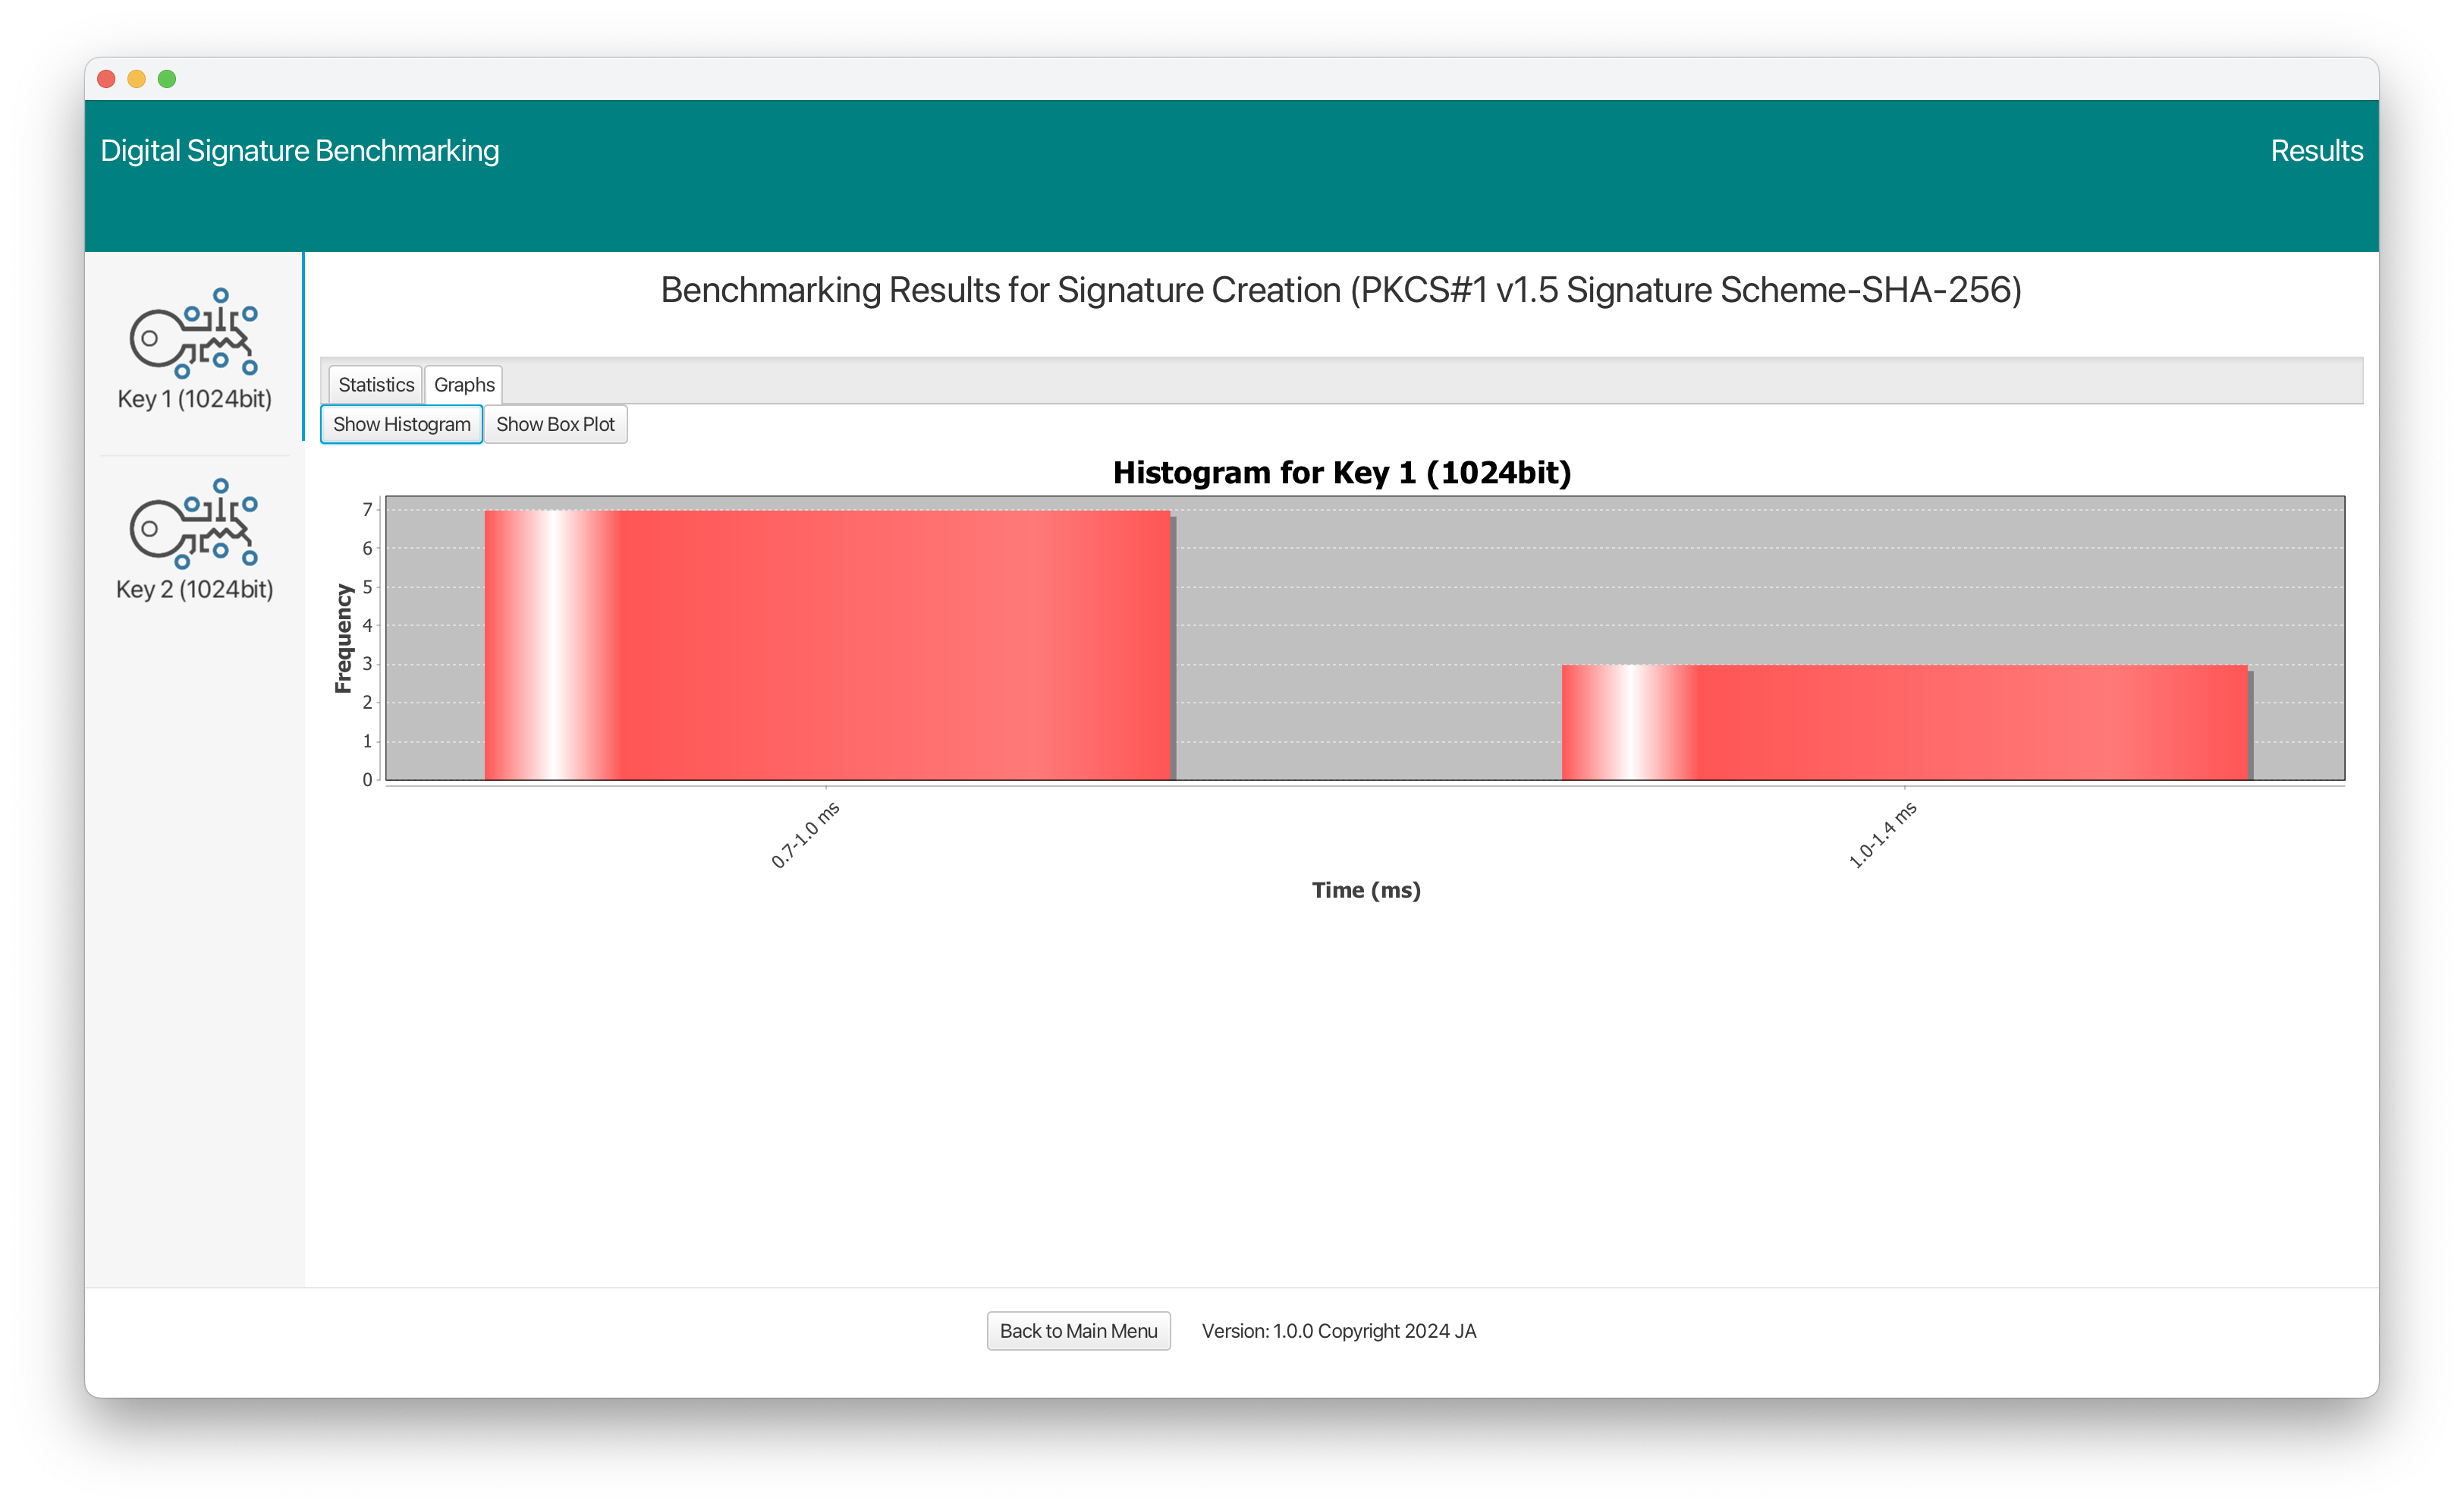
\includegraphics[width=\textwidth]{main_pictures/ui/signing/benchmarking/signing7.png}} % Adding border here
       \caption{Benchmarking: Signature Generation: Histogram}
        \label{fig:image1}
    \end{minipage}
    \hfill % Add some space between the images
    % Second image in a minipage
    \begin{minipage}{0.7\textwidth}
        \centering
        \fbox{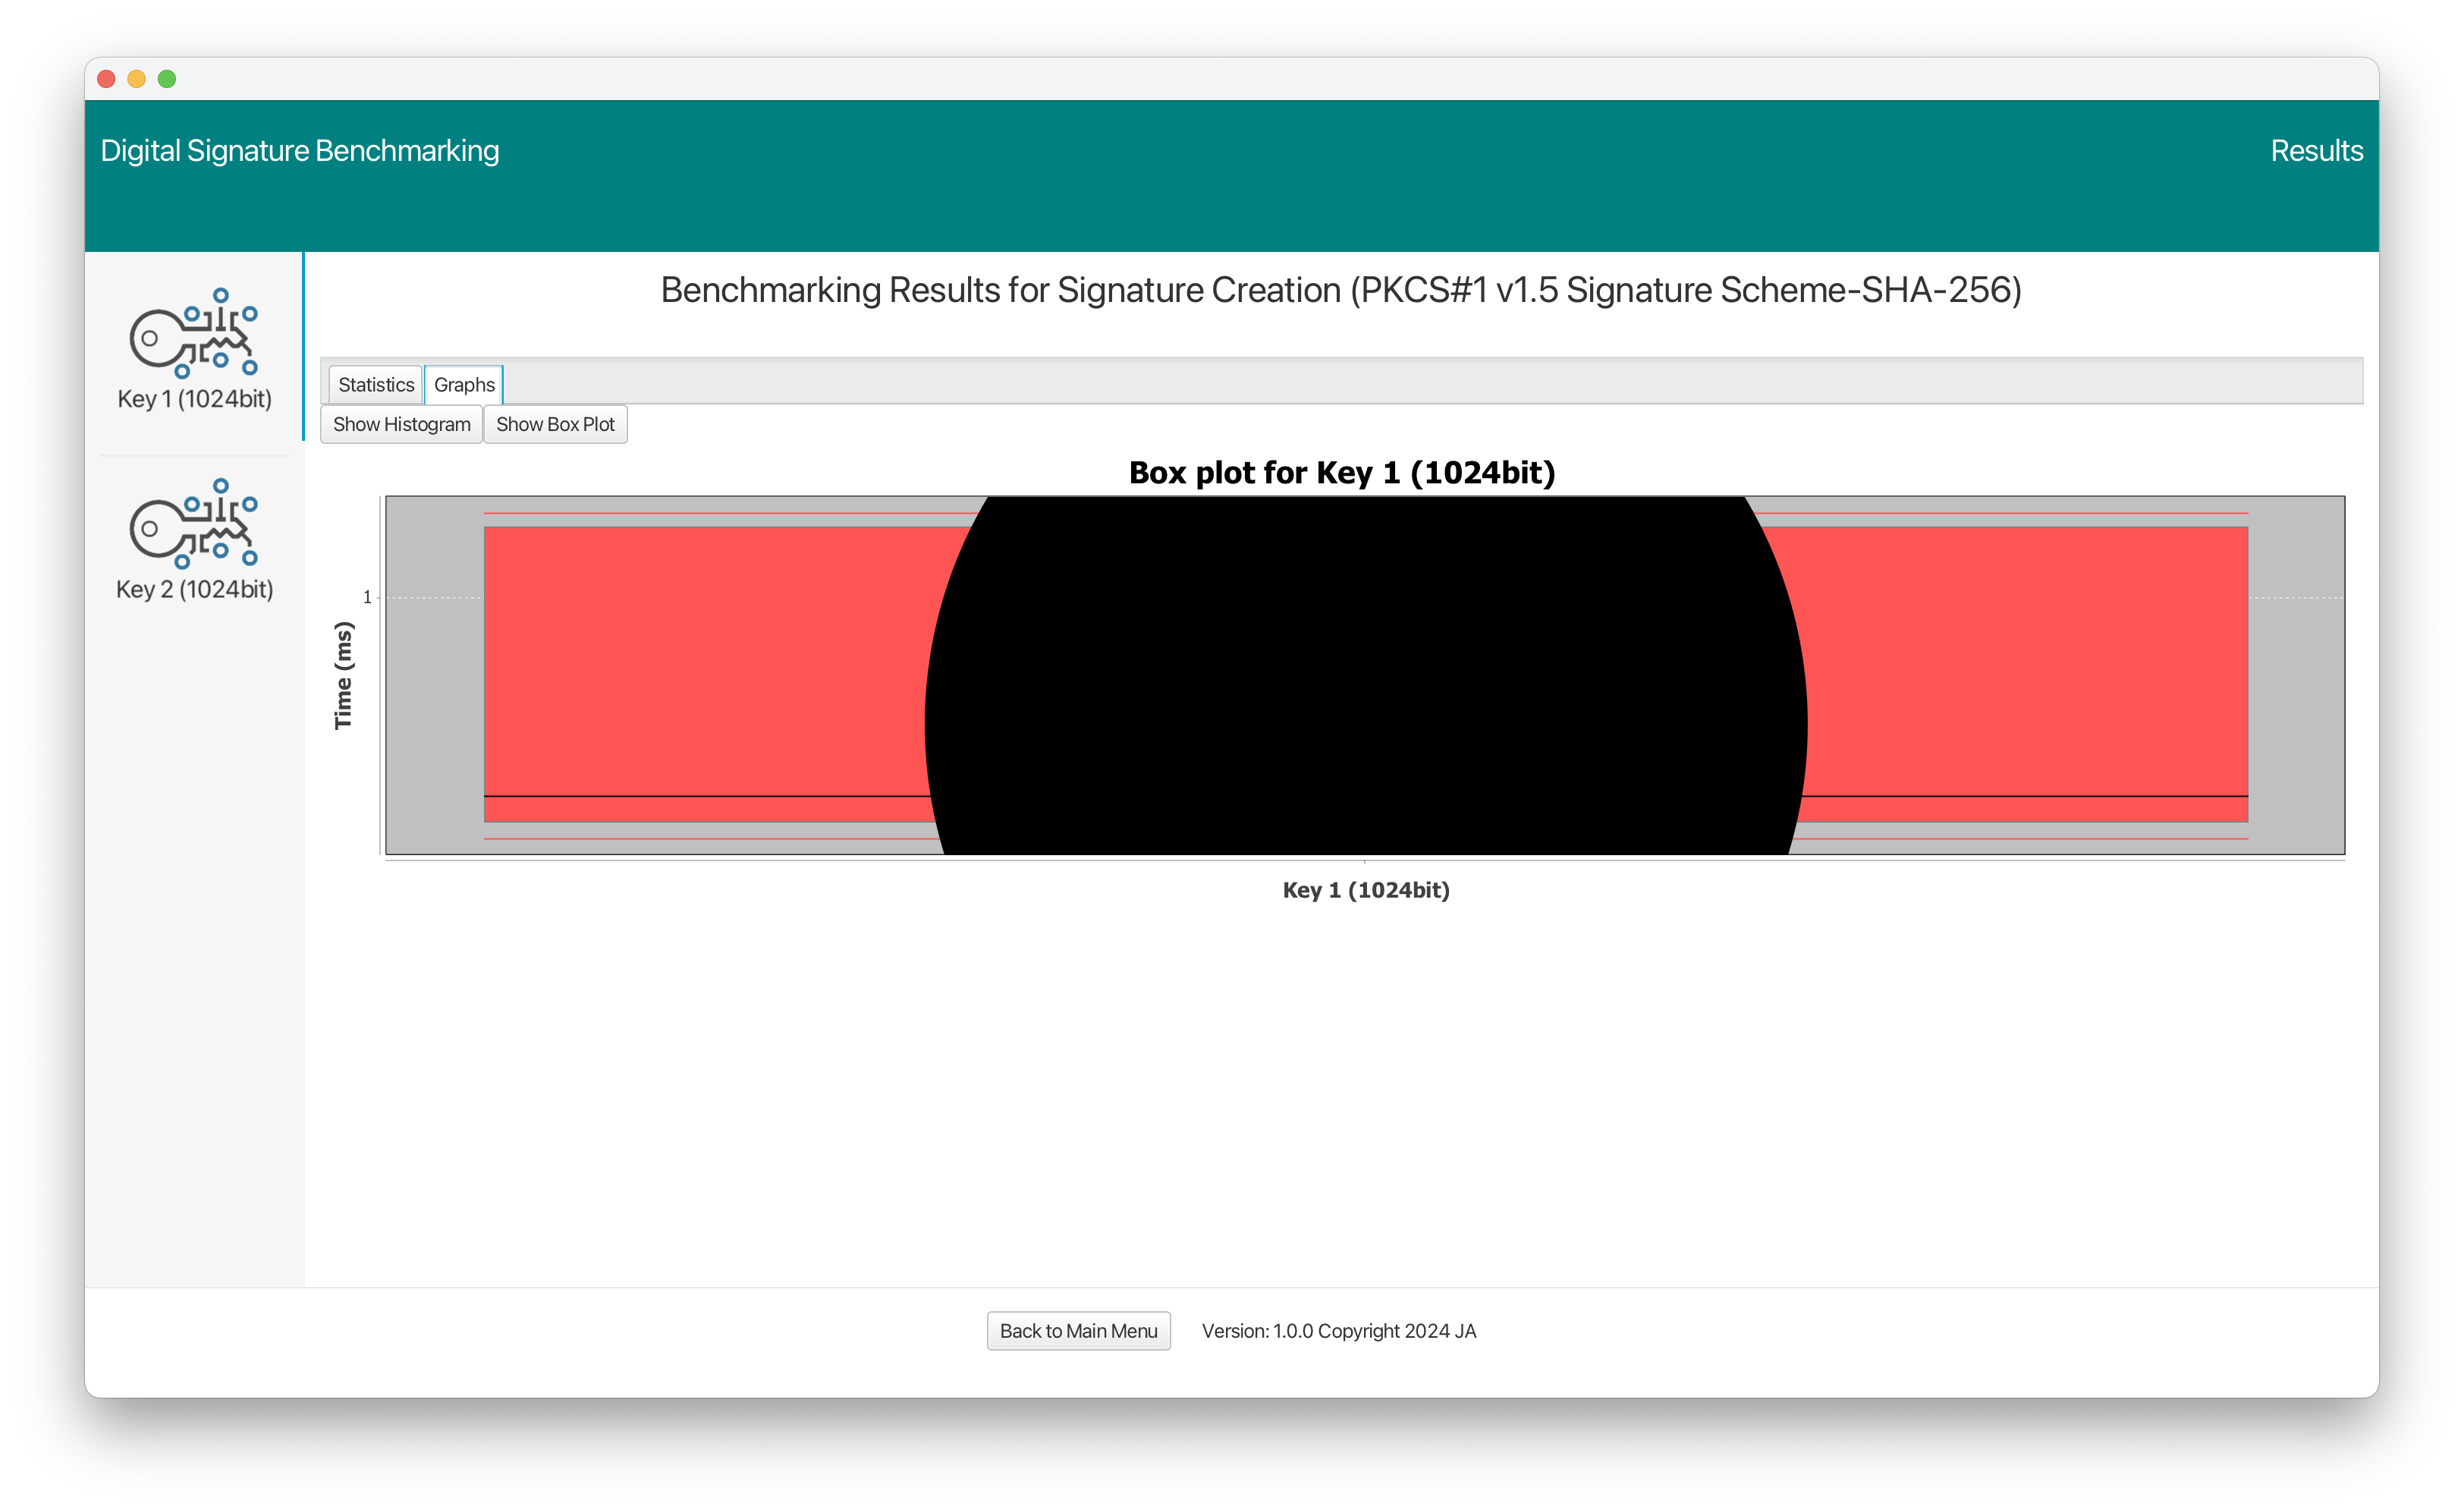
\includegraphics[width=\textwidth]{main_pictures/ui/signing/benchmarking/signing8.png}} % Adding border here
       \caption{Benchmarking: Signature Generation: Box plot graph}
        \label{fig:image2}
    \end{minipage}
 \end{figure}

Signature generation results can also be visualised graphically, accessible under the "Graphs" tab in the central pane. These graphs which correlate with data relevant to the currently selected key, offer an alternate method for interpreting the results.


\subsection{Signature Verification}


\begin{figure}[H]
    \centering % Center the images
    
    % First image in a minipage
    \begin{minipage}{0.4\textwidth}
        \centering
        \fbox{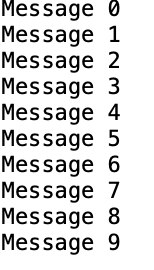
\includegraphics[width=0.4\textwidth]{main_pictures/ui/signing/signing2.png}} % Adding border here
       \caption{Benchmarking: Signature Verification (Test message batch (testMessages.txt))}
        \label{fig:image1}
    \end{minipage}
    \hfill % Add some space between the images
    % Second image in a minipage
    \begin{minipage}{0.58\textwidth}
        \centering
        \fbox{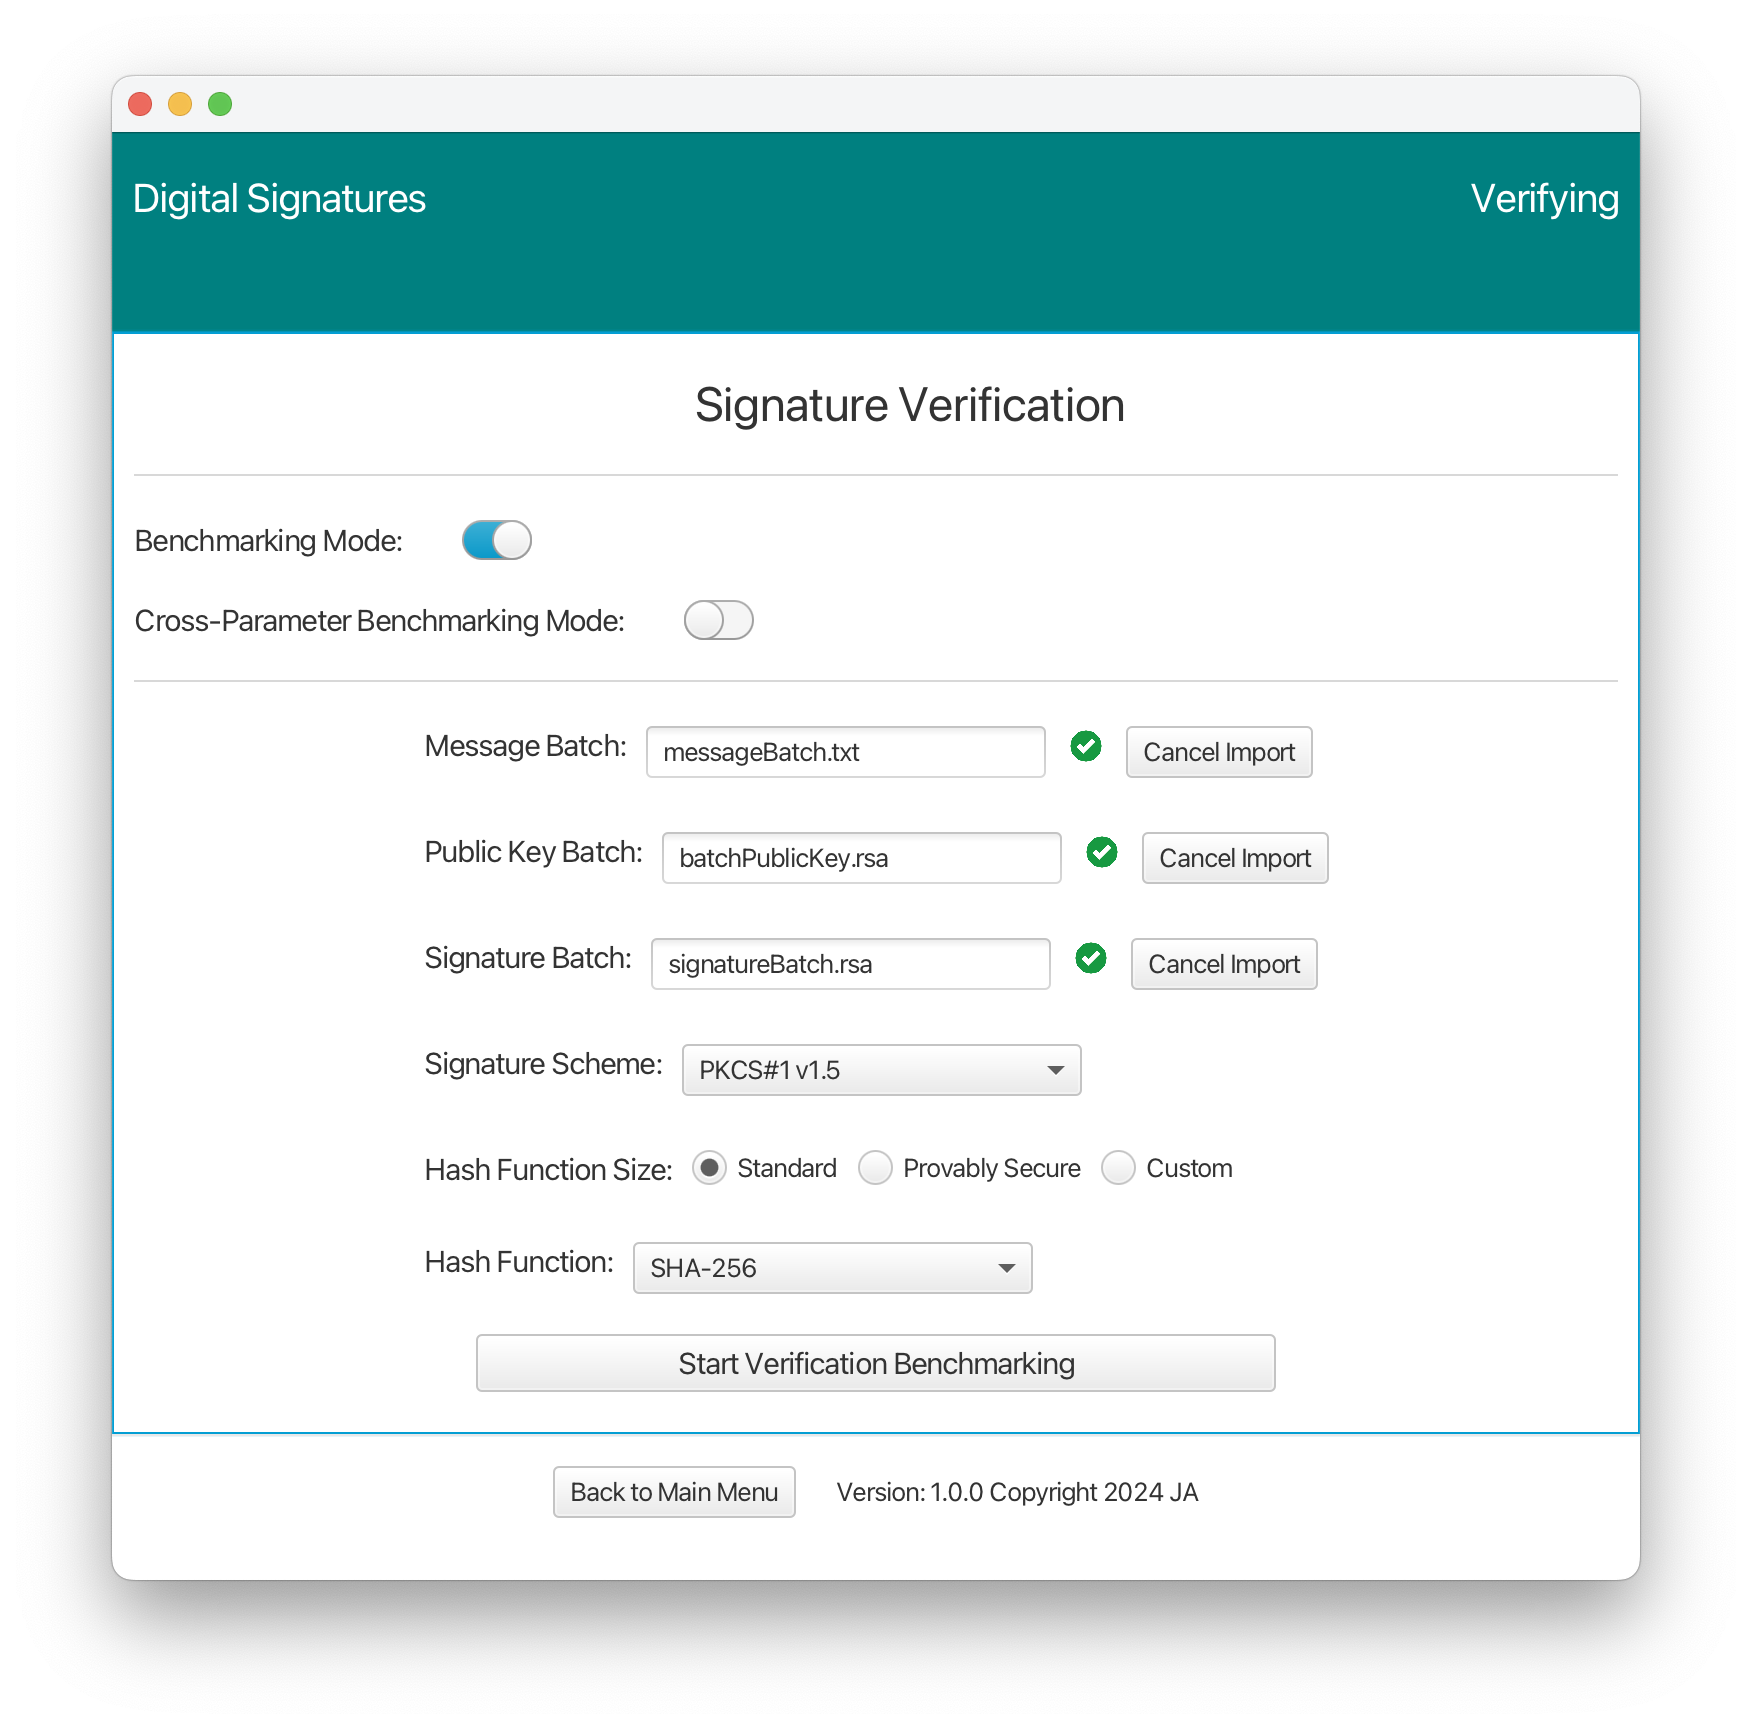
\includegraphics[width=\textwidth]{main_pictures/ui/verifying/benchmarking/verifying1.png}} % Adding border here
       \caption{Benchmarking: Signature Verification (Imported message batch)}
        \label{fig:image2}
    \end{minipage}
\end{figure}

Similar to the process for signature generation, the initial signature verification screen for benchmarking mode is displayed by default when selecting the relevant option from main menu on application launch. It includes fields for importing, key, message and signature batches. For correctness, it's necessary that the submitted message batch aligns with the submitted signature batch. Moreover, these batches must be compatible with the public key batch, which, in turn, is associated with the private key batch employed during the prior signature generation phase.

In signature verification benchmarking, hash function selected must align with the one used in signature generation to ensure correctness. 

Upon selecting "Start Verification Benchmarking," the application validates the number of signatures against the message batch and chosen hash functions.  Following successful validation,  verification benchmarking is executed . This involves comparing the signature batch with the message batch and public keys, using the selected signature scheme and hash functions. The process generates batches of verification results for each entered key size, and a progress bar provides real-time progress updates.

\newpage
\textbf{Benchmarking: Signature Verification Results Screen}

\begin{figure}[H]
    \centering
    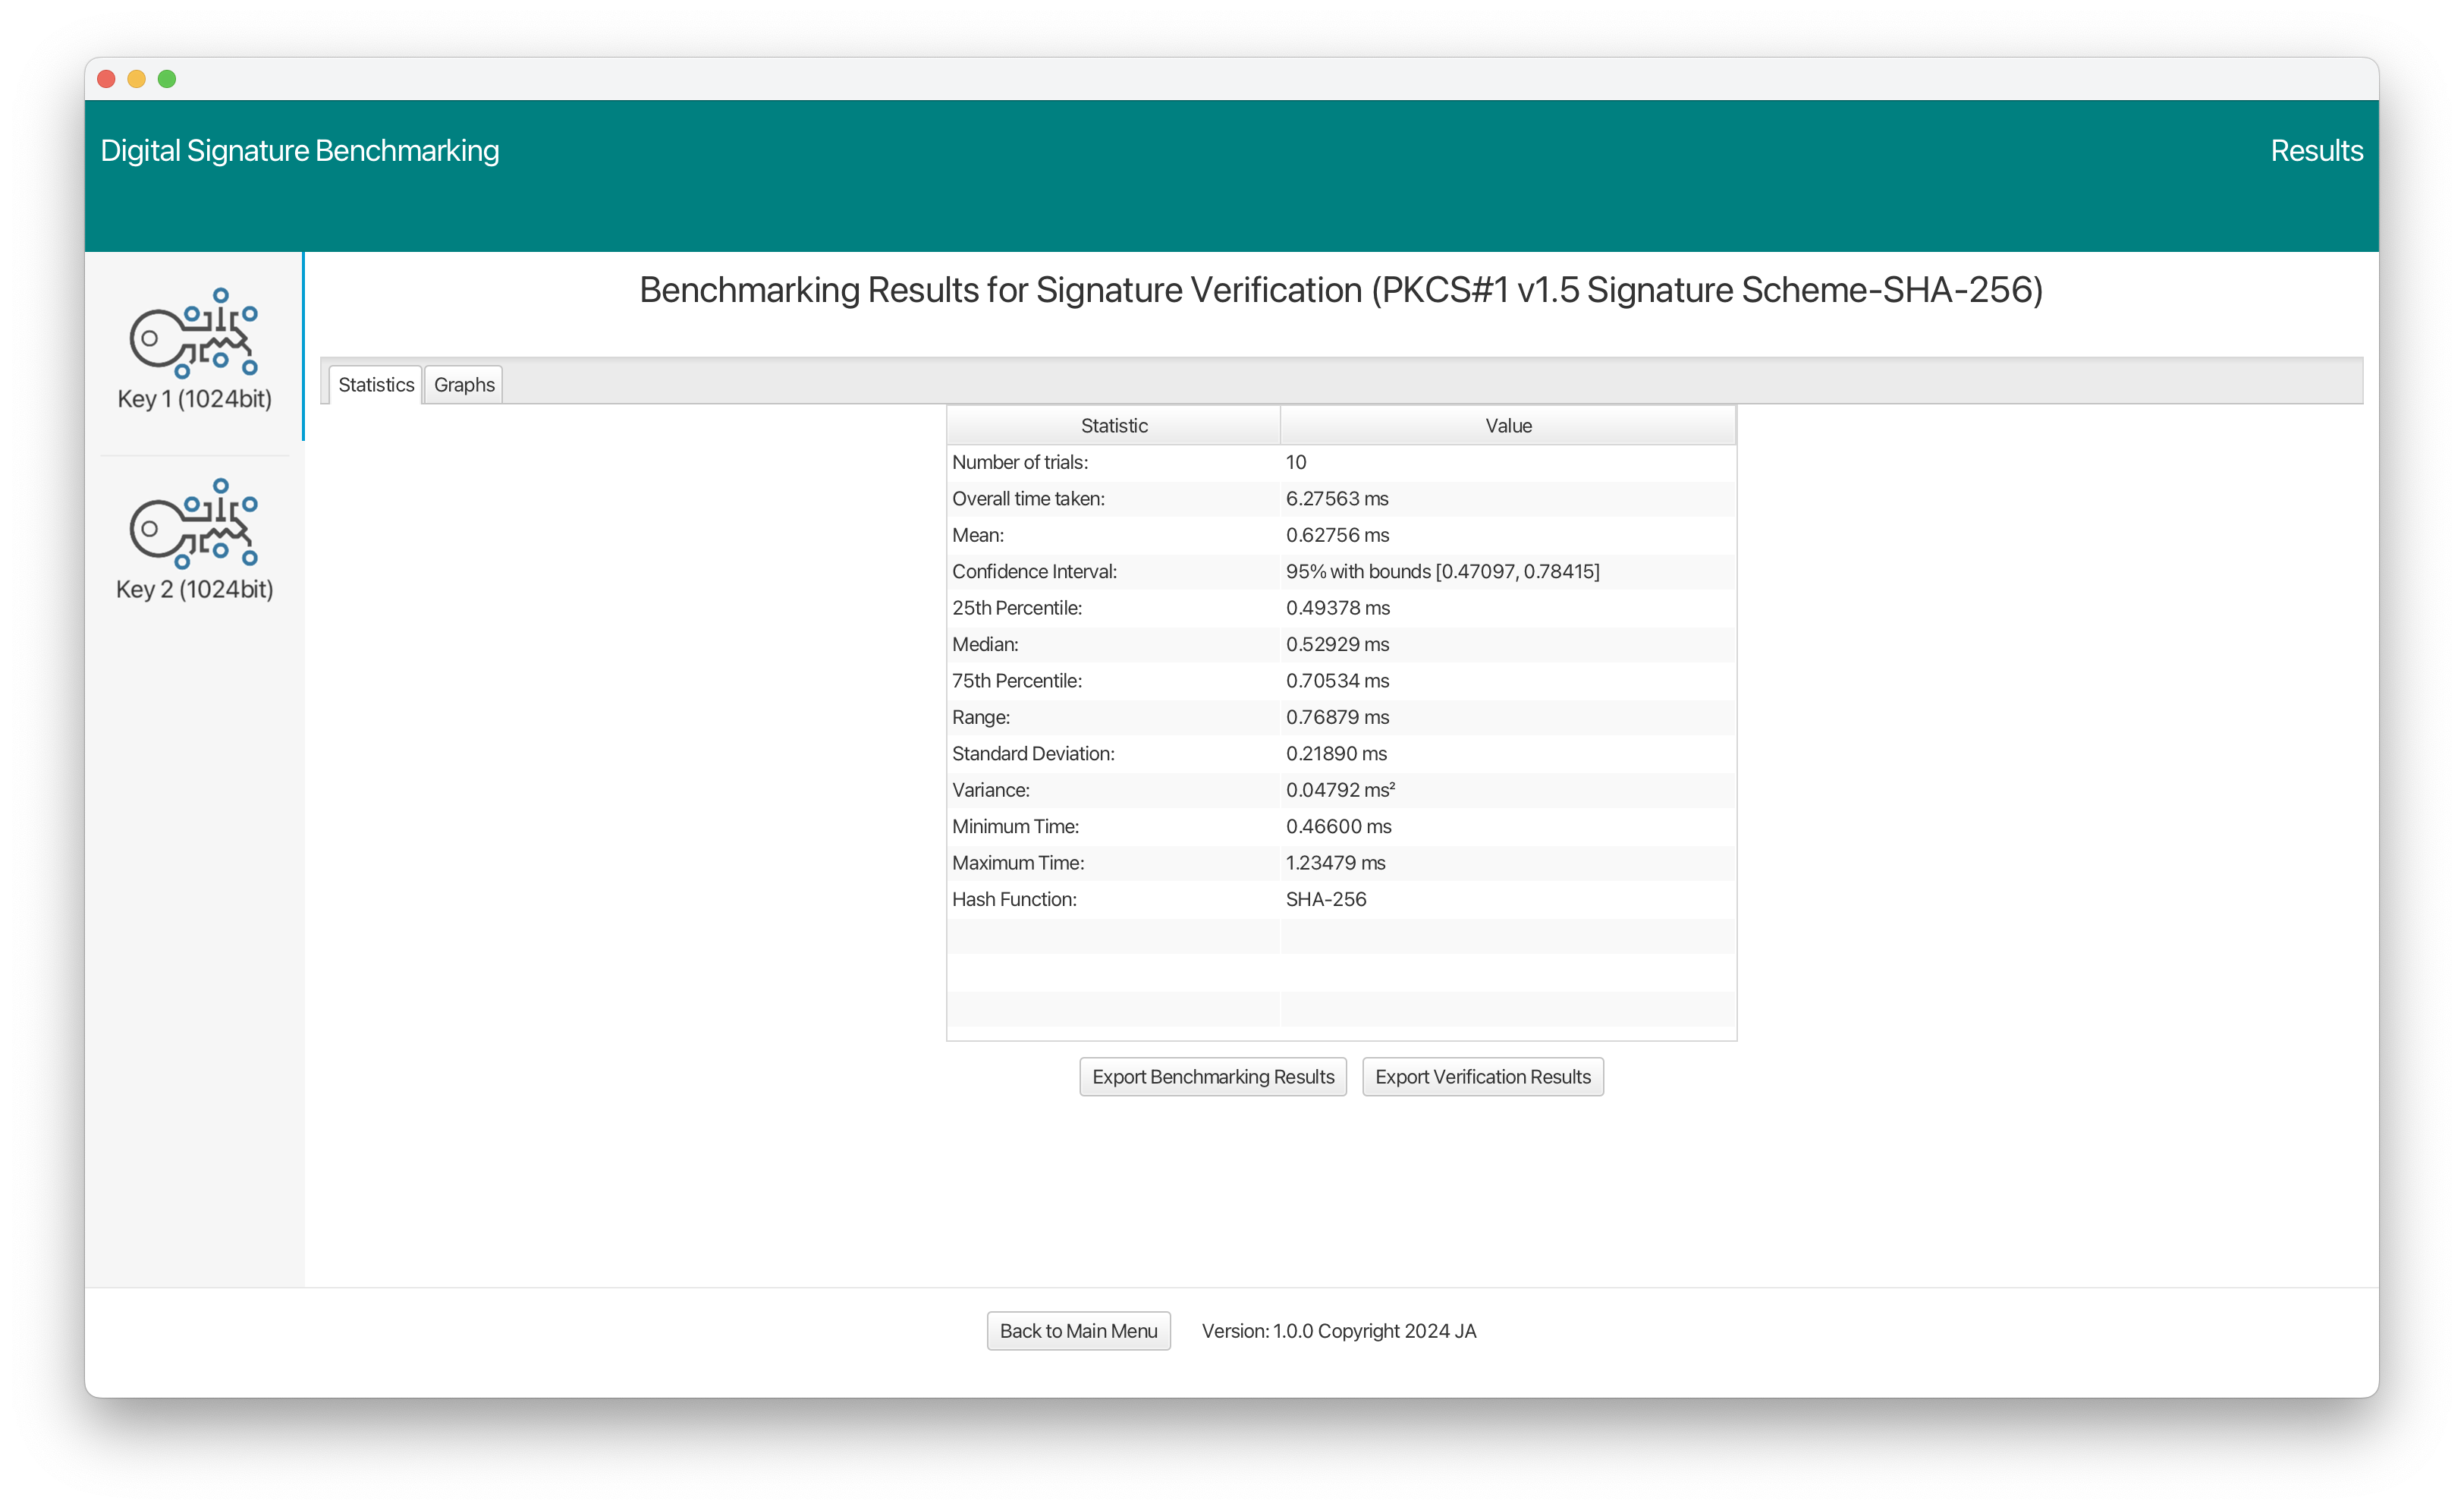
\includegraphics[scale= 0.325]{main_pictures/ui/verifying/benchmarking/verifying2.png}
   \caption{Benchmarking: Signature Verification (Results Screen)}
\end{figure}

Once the signature verification benchmarking concludes, results from benchmarking are displayed. The layout of this results screen is largely as was shown for signature generation. The distinction is the enabling of the export of verification results for each key displayed below each results table.



\chapter{Comparison Benchmarking (Standard vs. Provably Secure)}
\subsection{Key Generation}
\begin{figure}[H]
    \centering % Center the images
    
    % First image in a minipage
    \begin{minipage}{0.495\textwidth}
        \centering
        \fbox{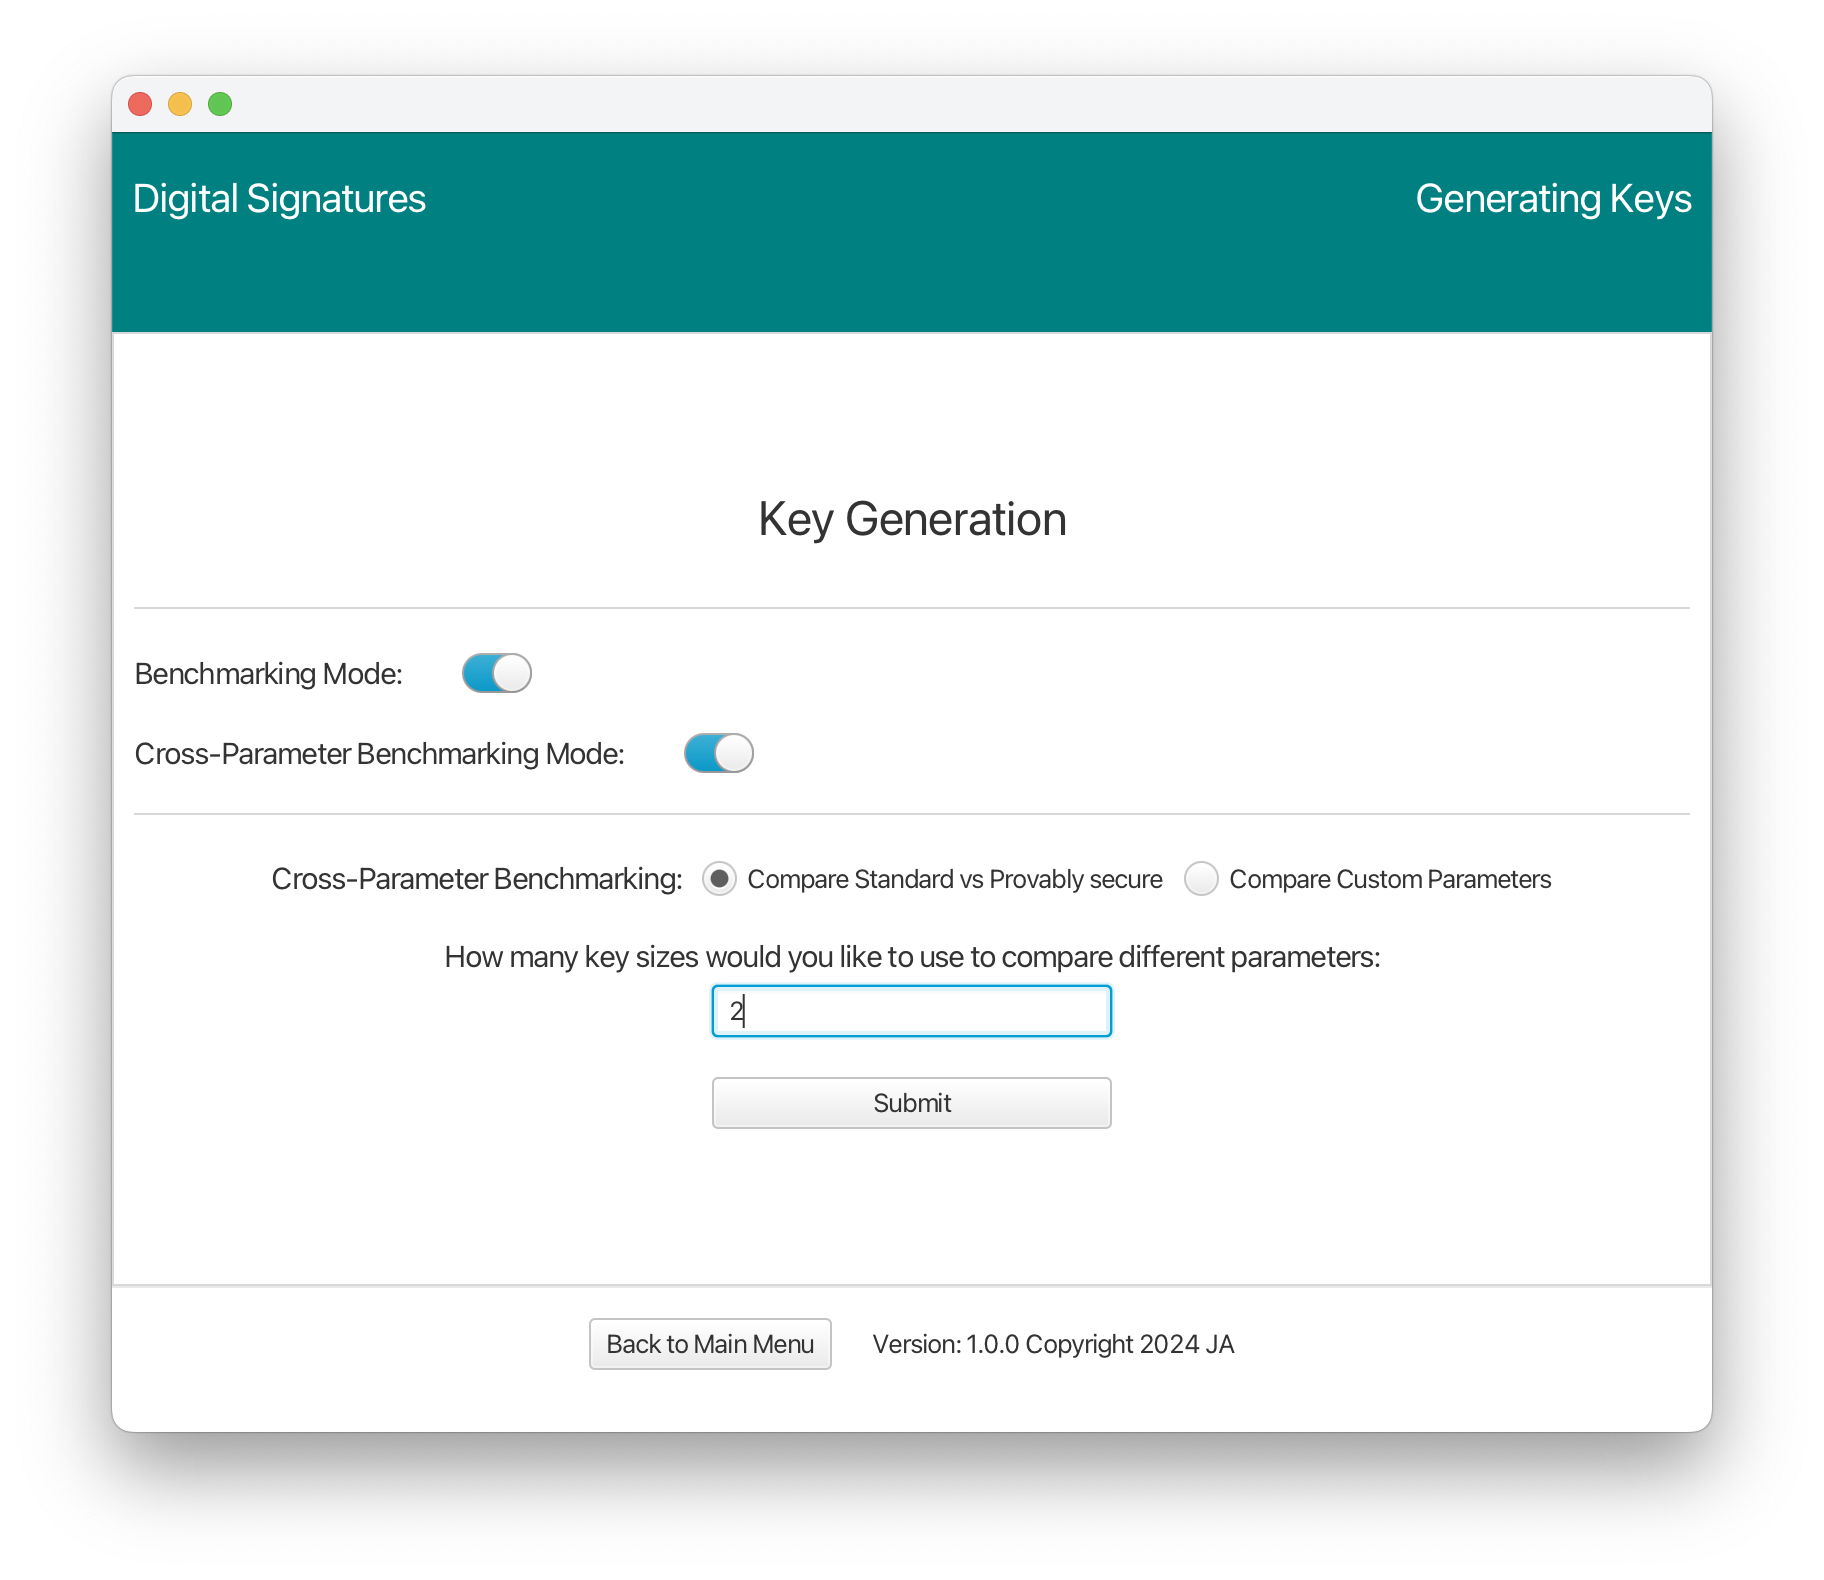
\includegraphics[width=\textwidth]{main_pictures/ui/keyGen/keyGen1.png}} % Adding border here
       \caption{Comparison Benchmarking: Key Generation (number of key sizes)}
        \label{fig:image1}
    \end{minipage}
    \hfill % Add some space between the images
    % Second image in a minipage
    \begin{minipage}{0.495\textwidth}
        \centering
        \fbox{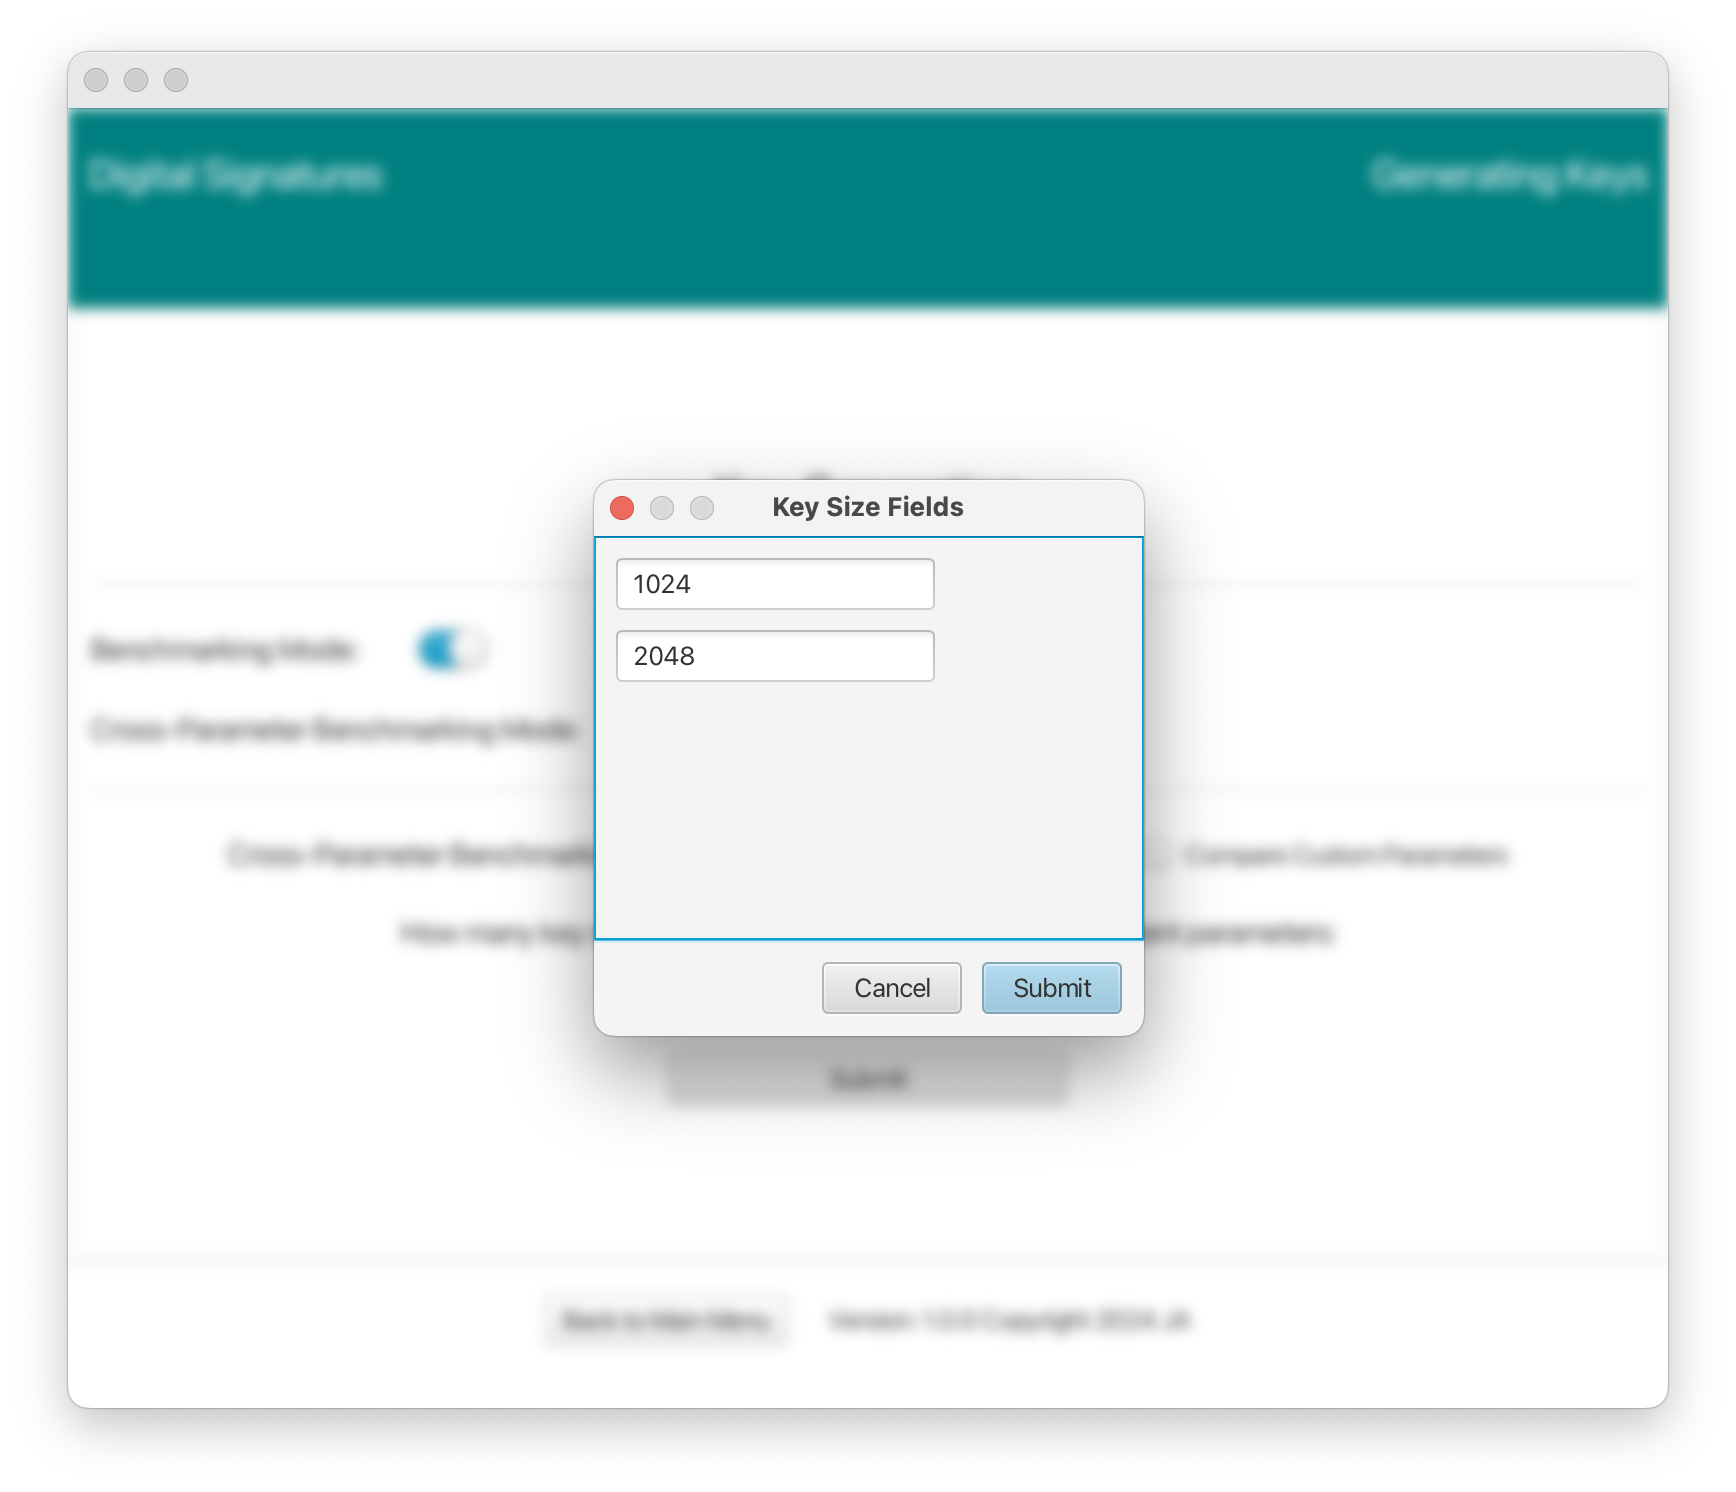
\includegraphics[width=\textwidth]{main_pictures/ui/keyGen/keyGen2.png}} % Adding border here
       \caption{Comparison Benchmarking: Key Generation (key sizes)}
        \label{fig:image2}
    \end{minipage}
    
     \begin{minipage}{0.55\textwidth}
        \centering
        \fbox{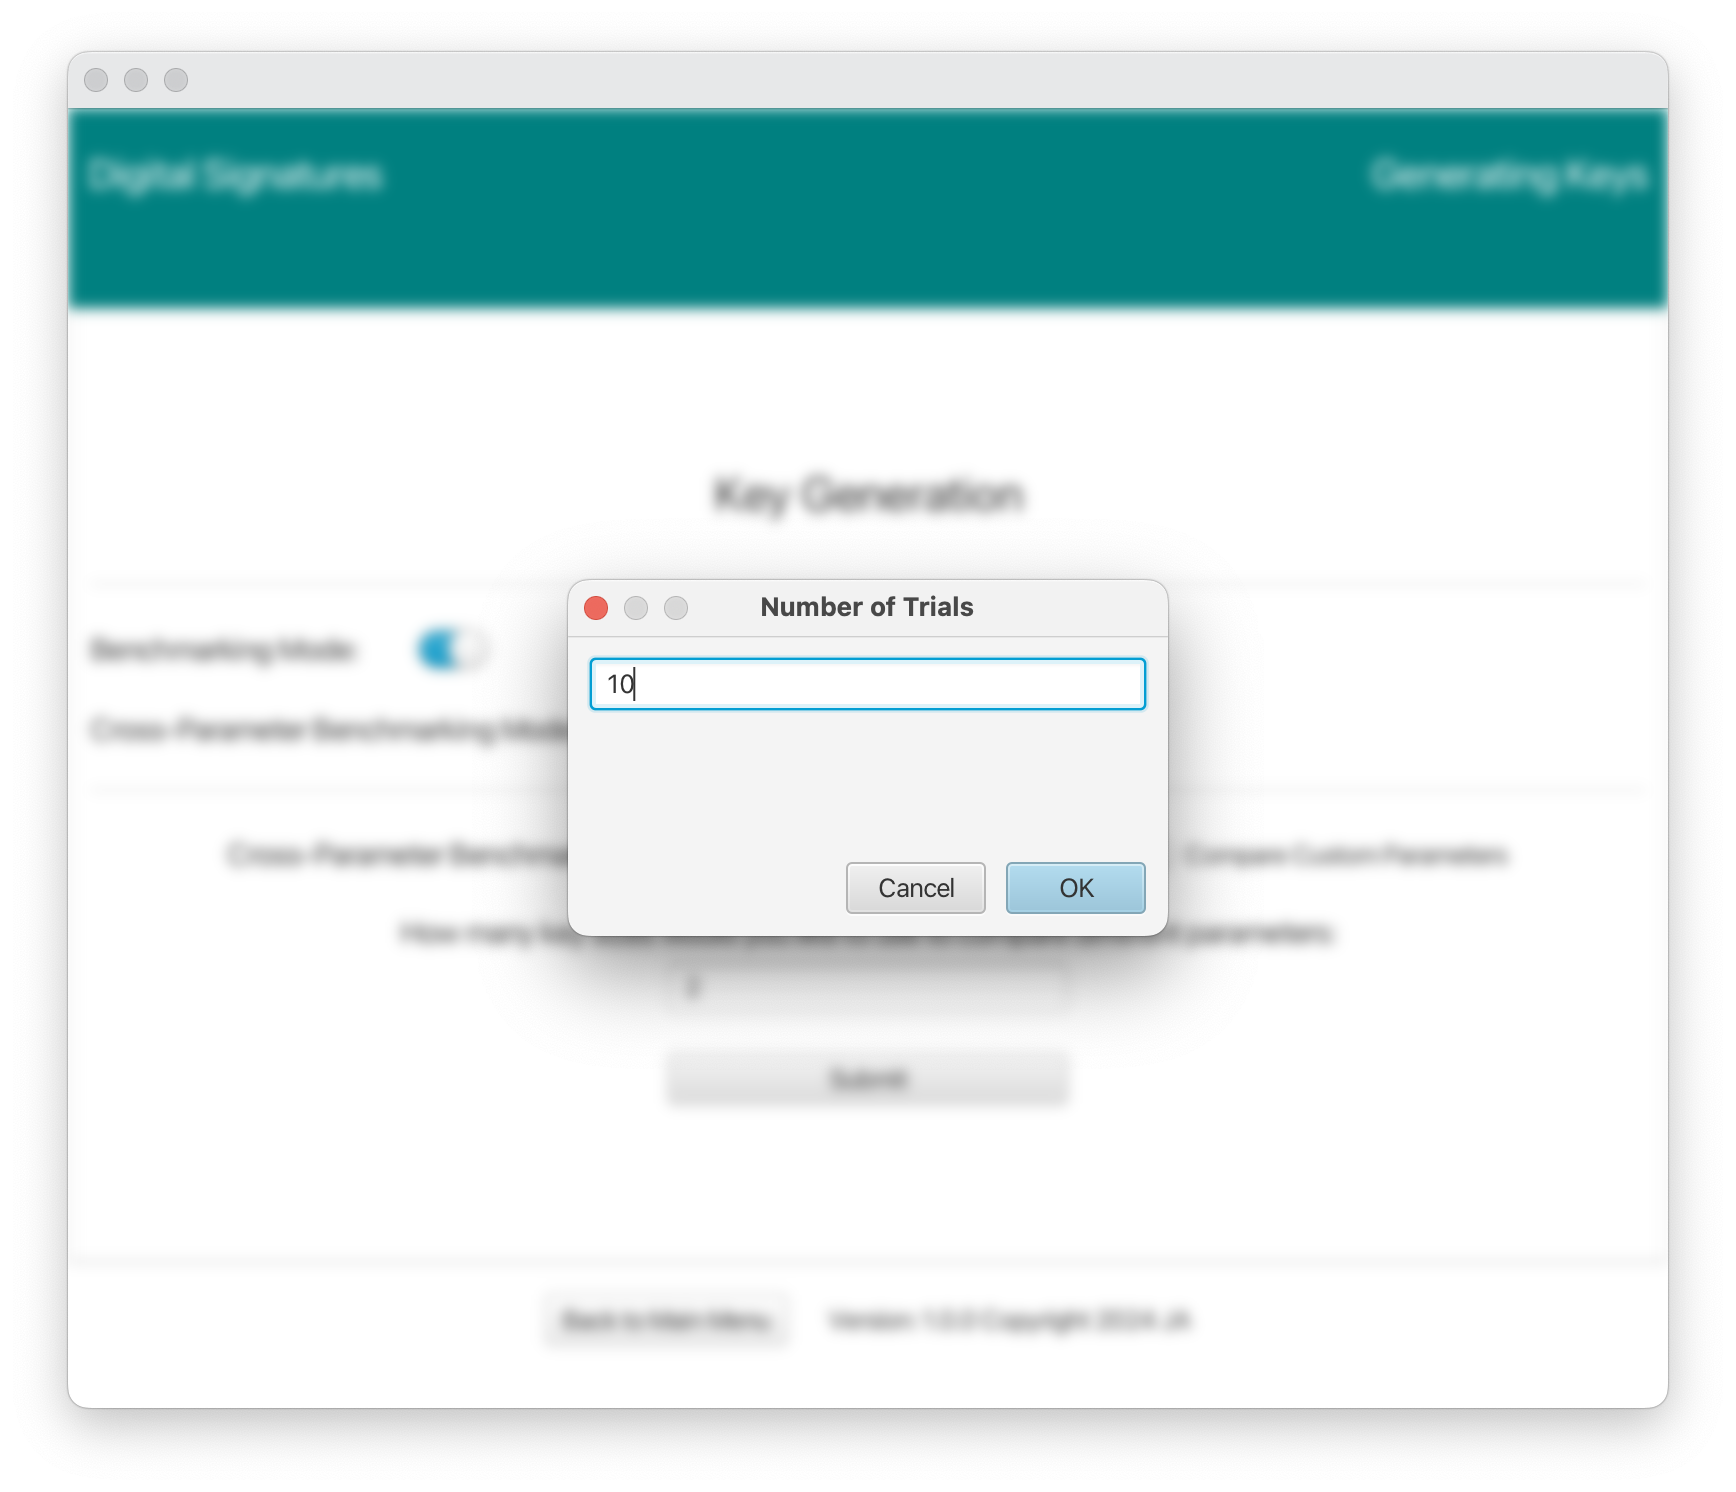
\includegraphics[width=\textwidth]{main_pictures/ui/keyGen/keyGen3.png}} % Adding border here
       \caption{Comparison Benchmarking: Key Generation (number of trials)}
        \label{fig:image2}
    \end{minipage}
\end{figure}
The key generation interface for comparison benchmarking is activated through a toggle switch. This interface offers a radio button to select the default comparison benchmarking mode, which compares standard and provably secure key configurations. Users specify the number of key sizes they wish to test, and corresponding input fields are displayed for each size (e.g., Key Size 1: 1024, Key Size 2: 2048).

For each entered key size, the application generates two groups of key configurations:
\begin{itemize}
    \item A \textbf{Standard Parameters} group, with both 2-prime and 3-prime modulus configurations and arbitrary e values.
    \item A \textbf{Provably Secure Parameters} group, with 2-prime and 3-prime modulus configurations and small e values.
\end{itemize}

Users then input the desired number of trials for key generation benchmarking, such as 10 trials. The application executes these trials for each of the four key configurations at the selected key sizes.

Clicking the "OK" button on the number of trials dialog sets the benchmarking process in motion. A progress bar is displayed for a length of time spanning the duration of the task allowing for real-time indication of progress.


\begin{figure}[H]
    \centering
    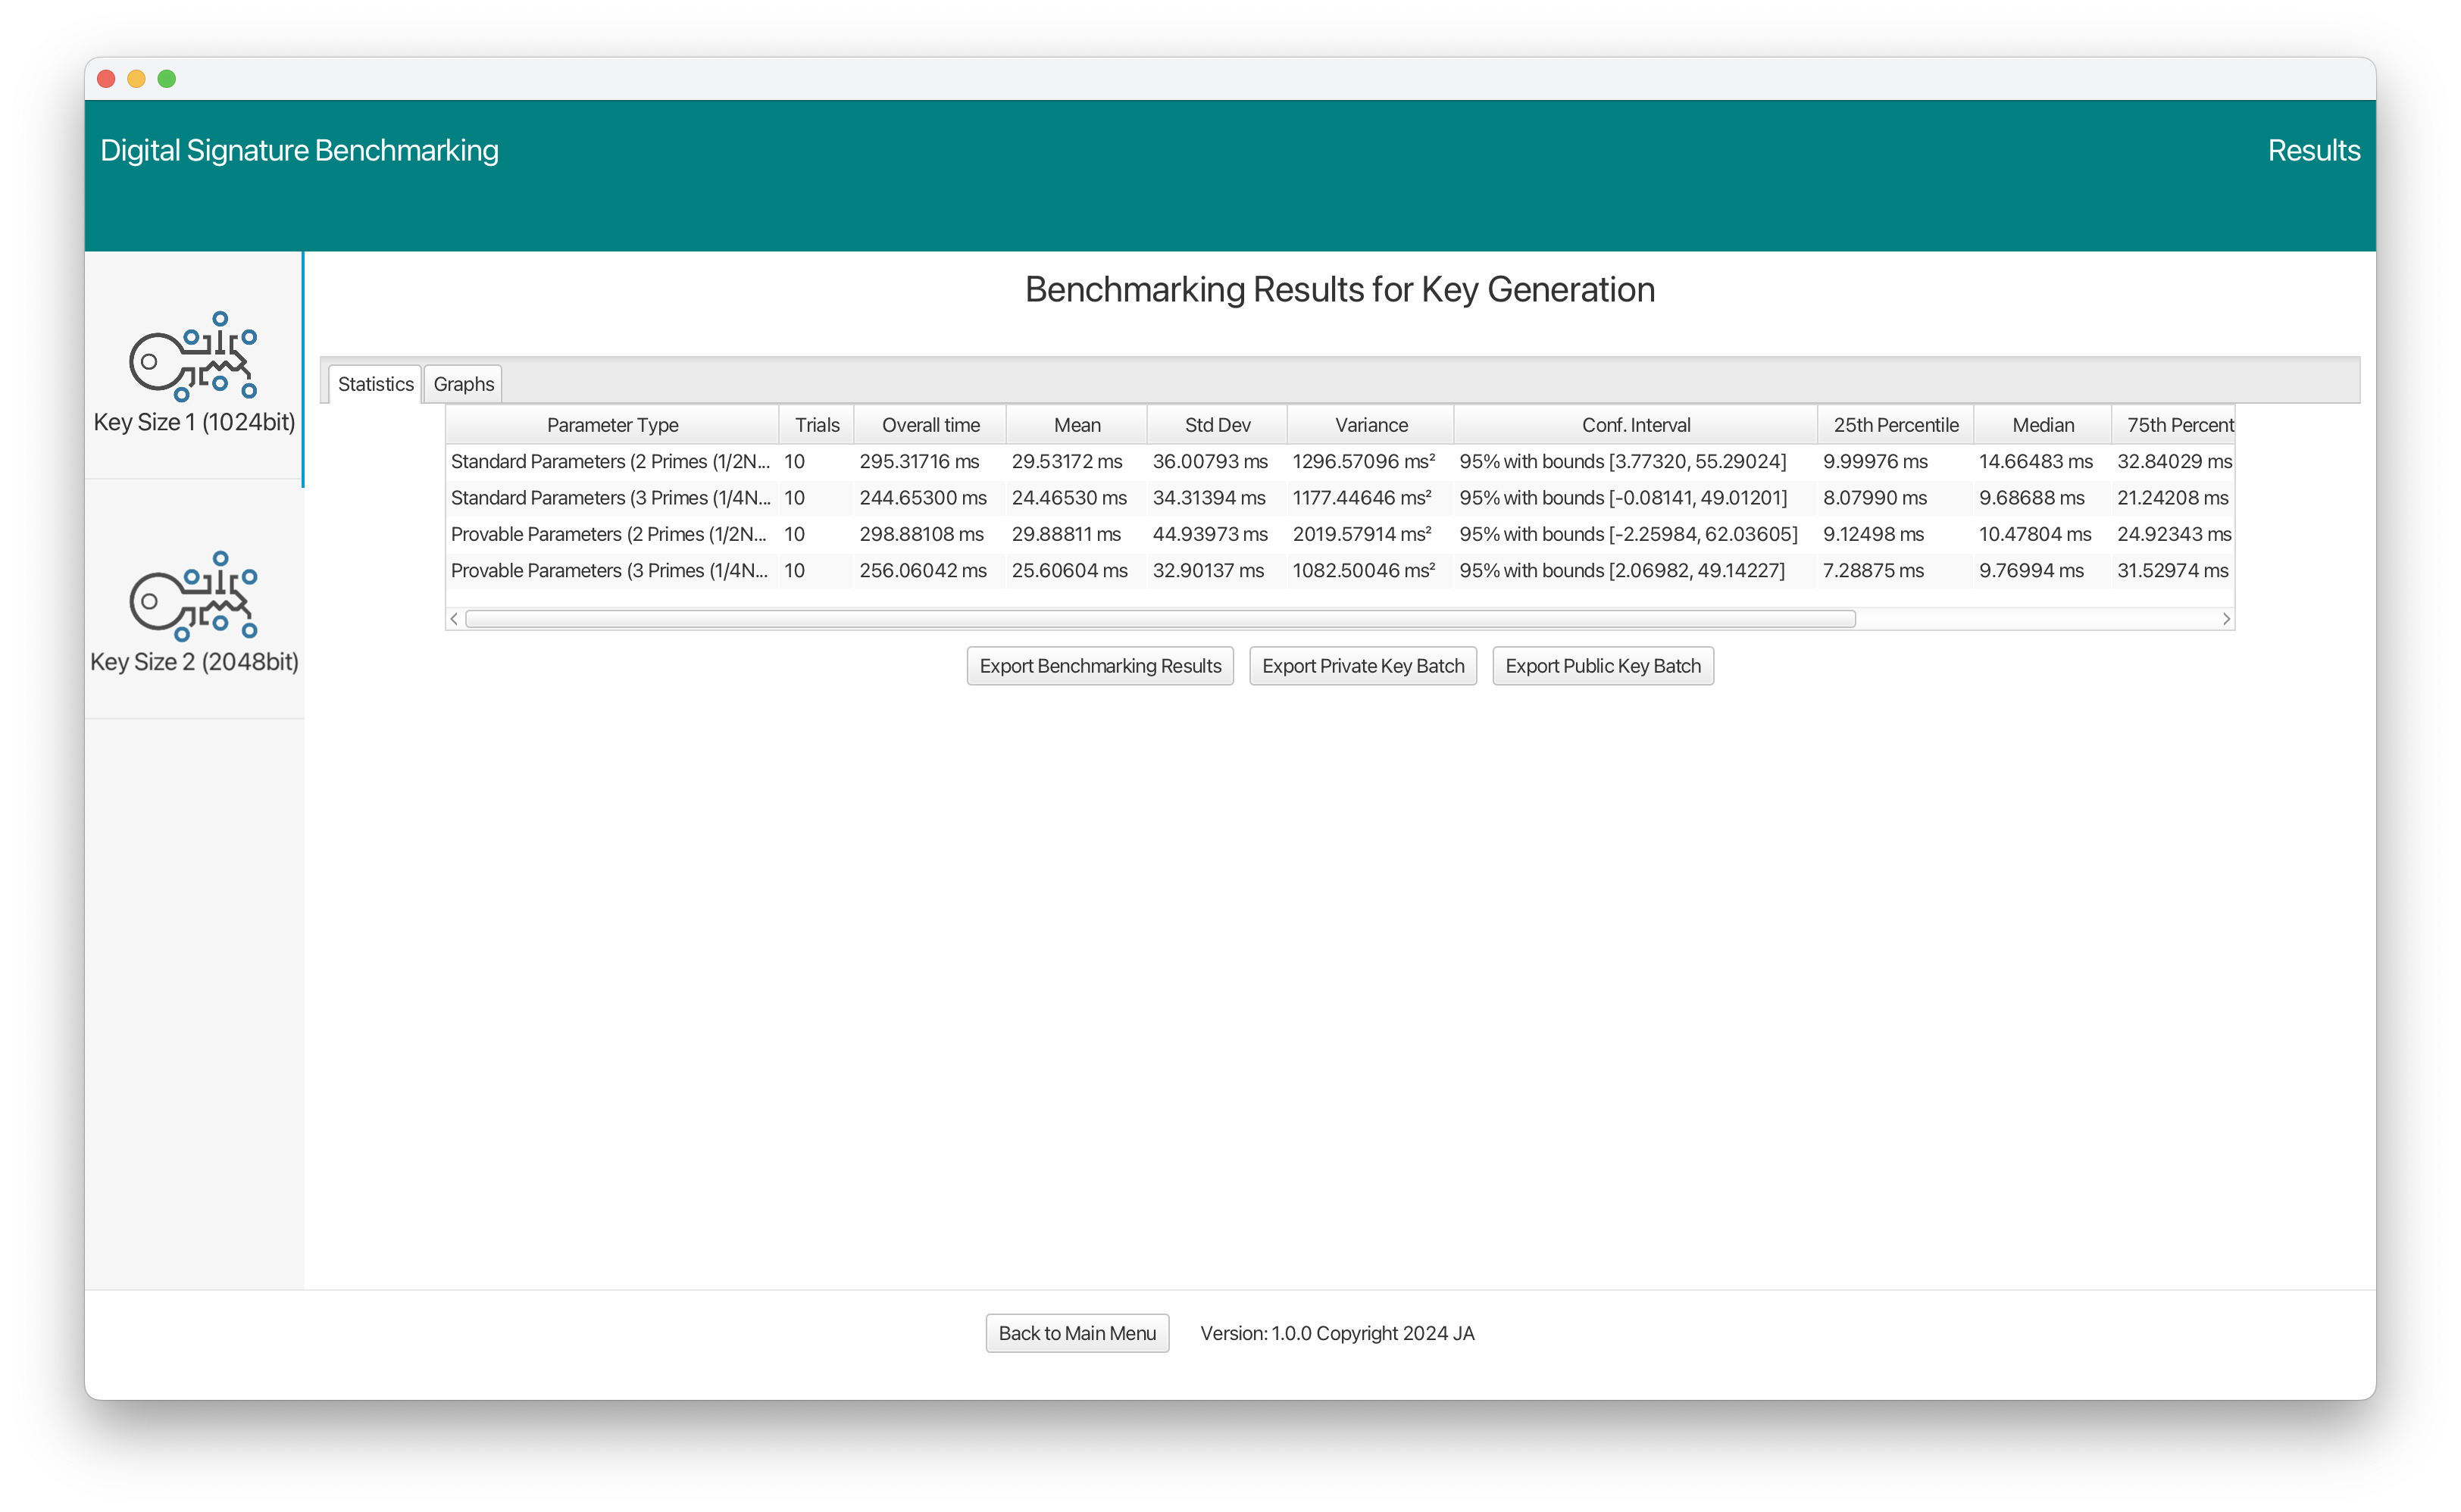
\includegraphics[scale= 0.325]{main_pictures/ui/keyGen/keyGen4.png}
   \caption{Comparison Benchmarking: Key Generation (Results Screen)}
\end{figure}
Upon completion of benchmarking, results from benchmarking are displayed. The results screen contains a side pane with buttons corresponding to each individual key size previously entered. Within each side tab, the results table displays a row by row sequence of statistical metrics for all 4 key configurations.  The ordering is by parameter set (i.e., 2 key configurations for standard parameter key results first, followed by the 2 key configurations for provably secure parameter results second). Below the results table, the application also provides the functionality to export the benchmarking results and if desired public or private key batches corresponding to a global set of keys matching the key configurations enumerated in a sequence for all key sizes.




\begin{figure}[H]
    \centering % Center the images
    
    % First image in a minipage
    \begin{minipage}{0.7\textwidth}
        \centering
        \fbox{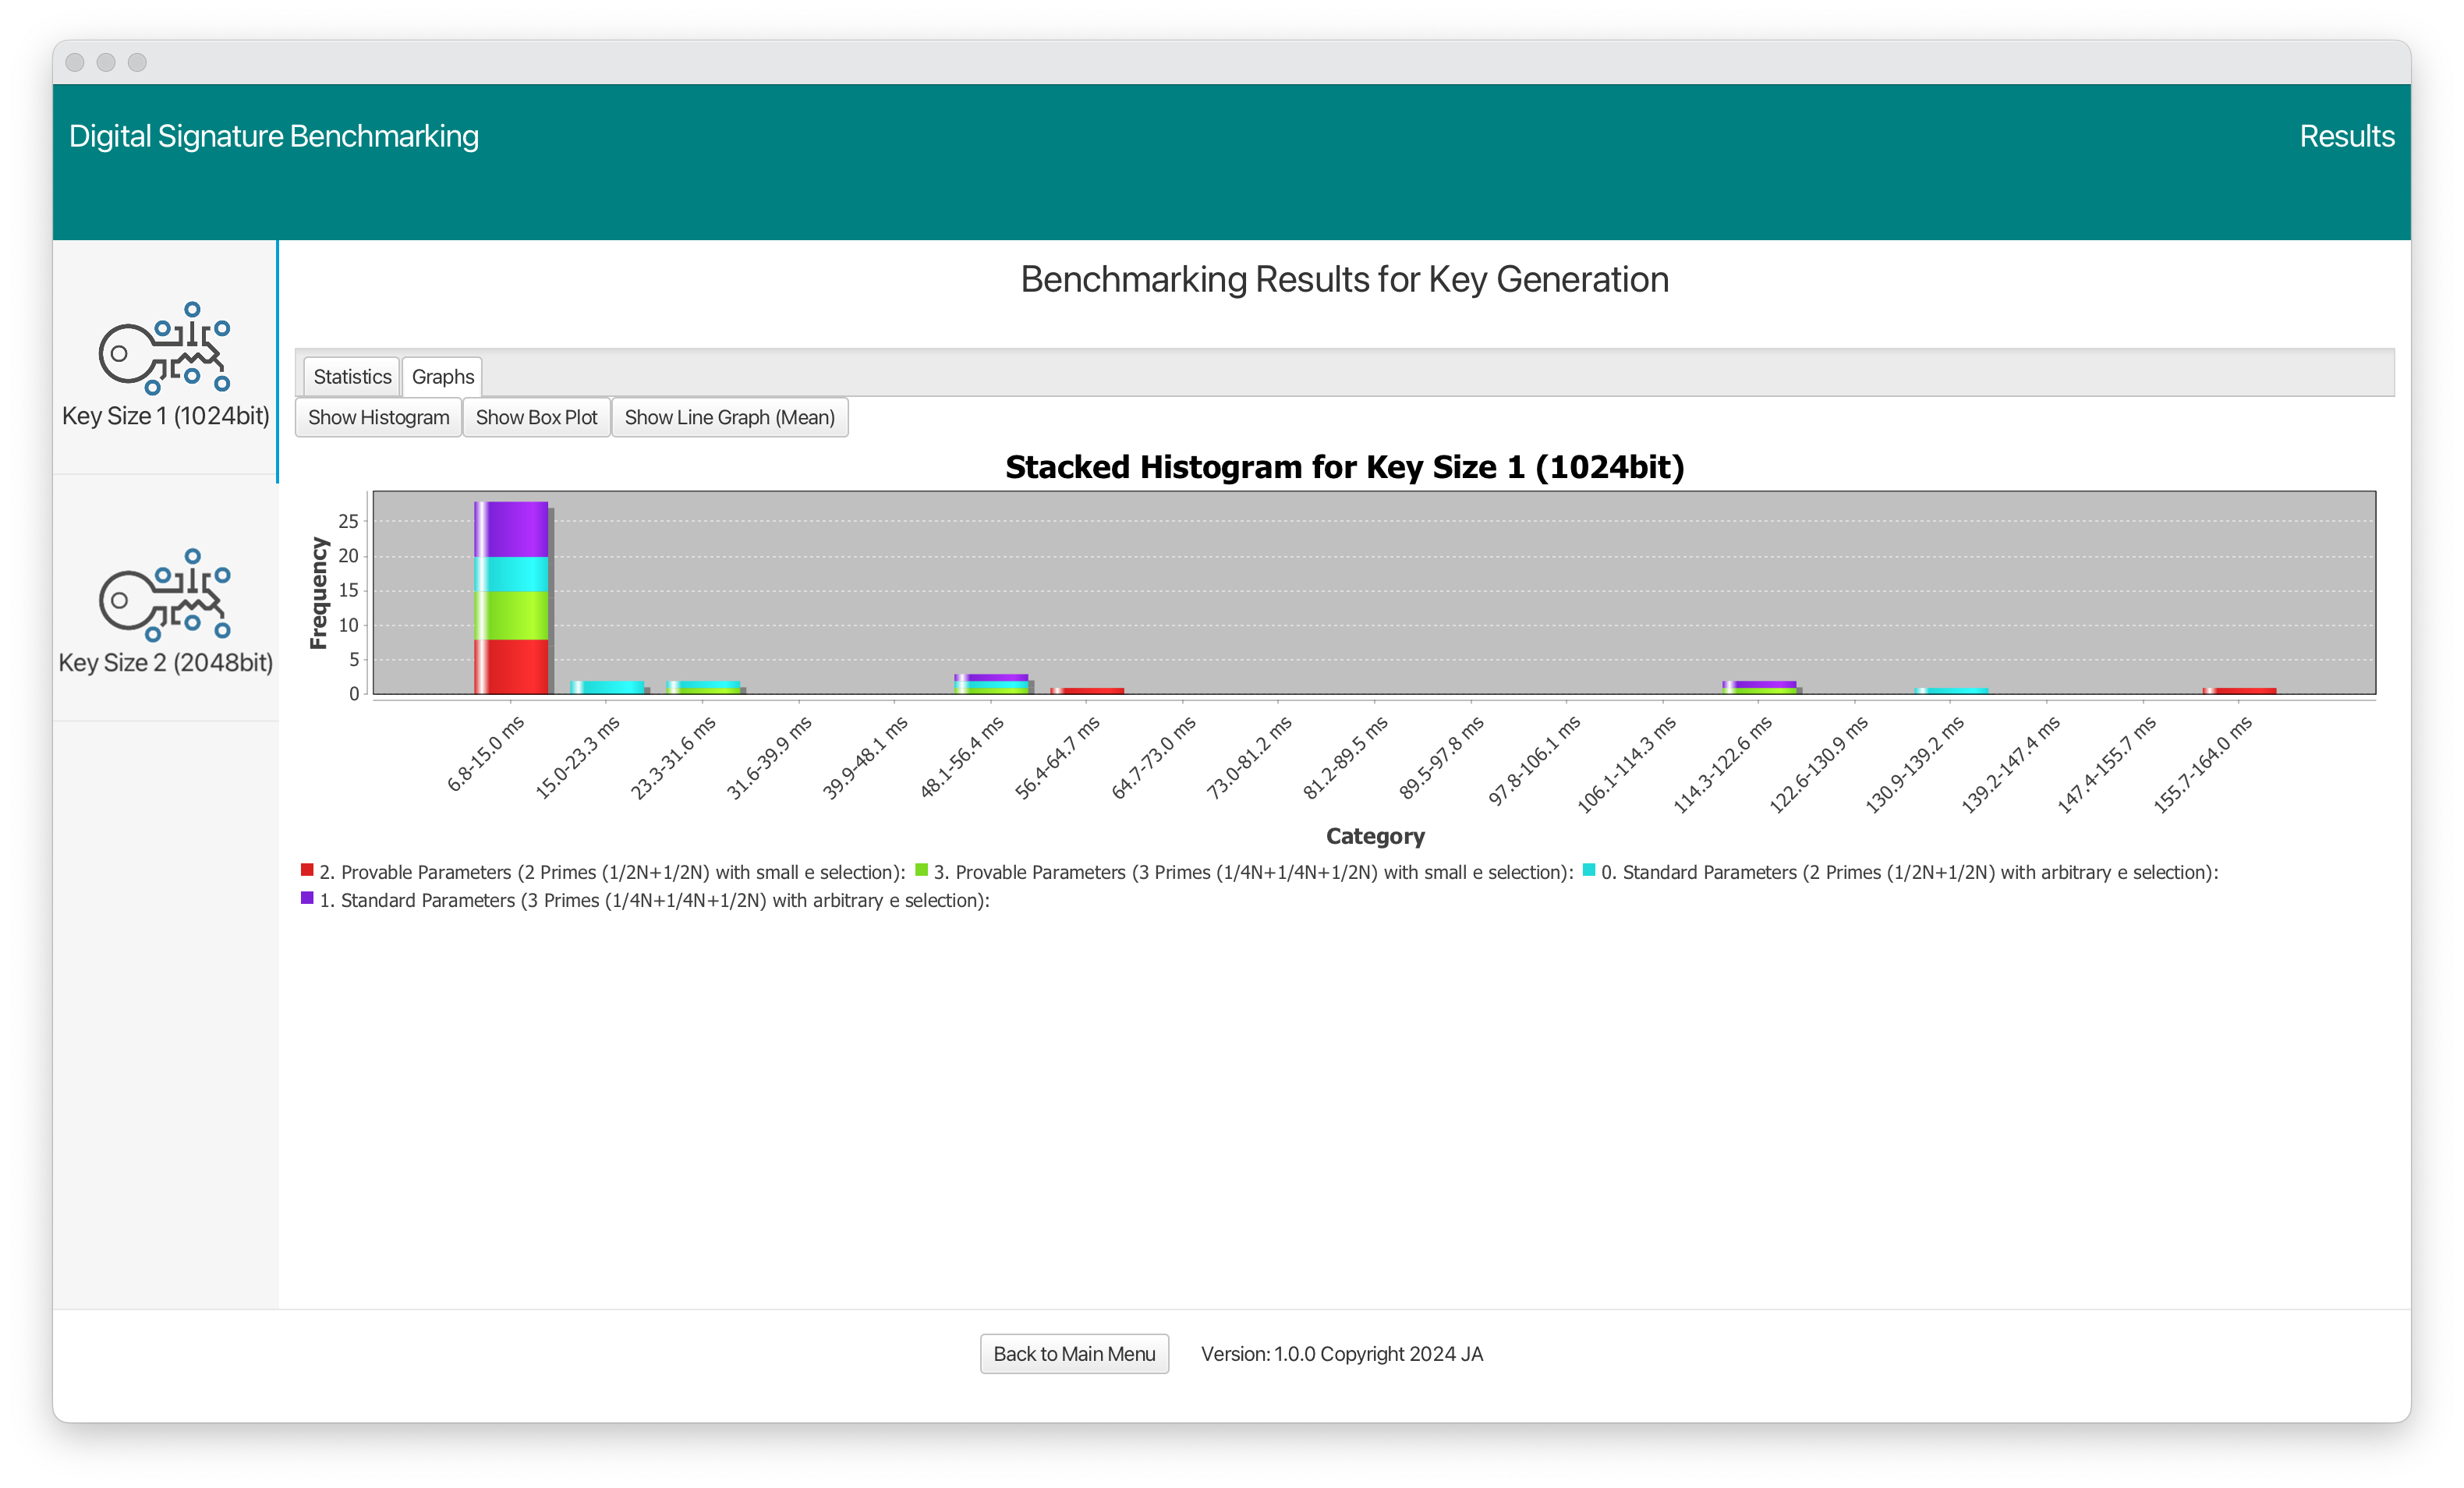
\includegraphics[width=\textwidth]{main_pictures/ui/keyGen/keyGen5.png}} % Adding border here
       \caption{Comparison Benchmarking: Key Generation: Overlaid Histogram}
        \label{fig:image1}
    \end{minipage}
    \hfill % Add some space between the images
    % Second image in a minipage
    \begin{minipage}{0.7\textwidth}
        \centering
        \fbox{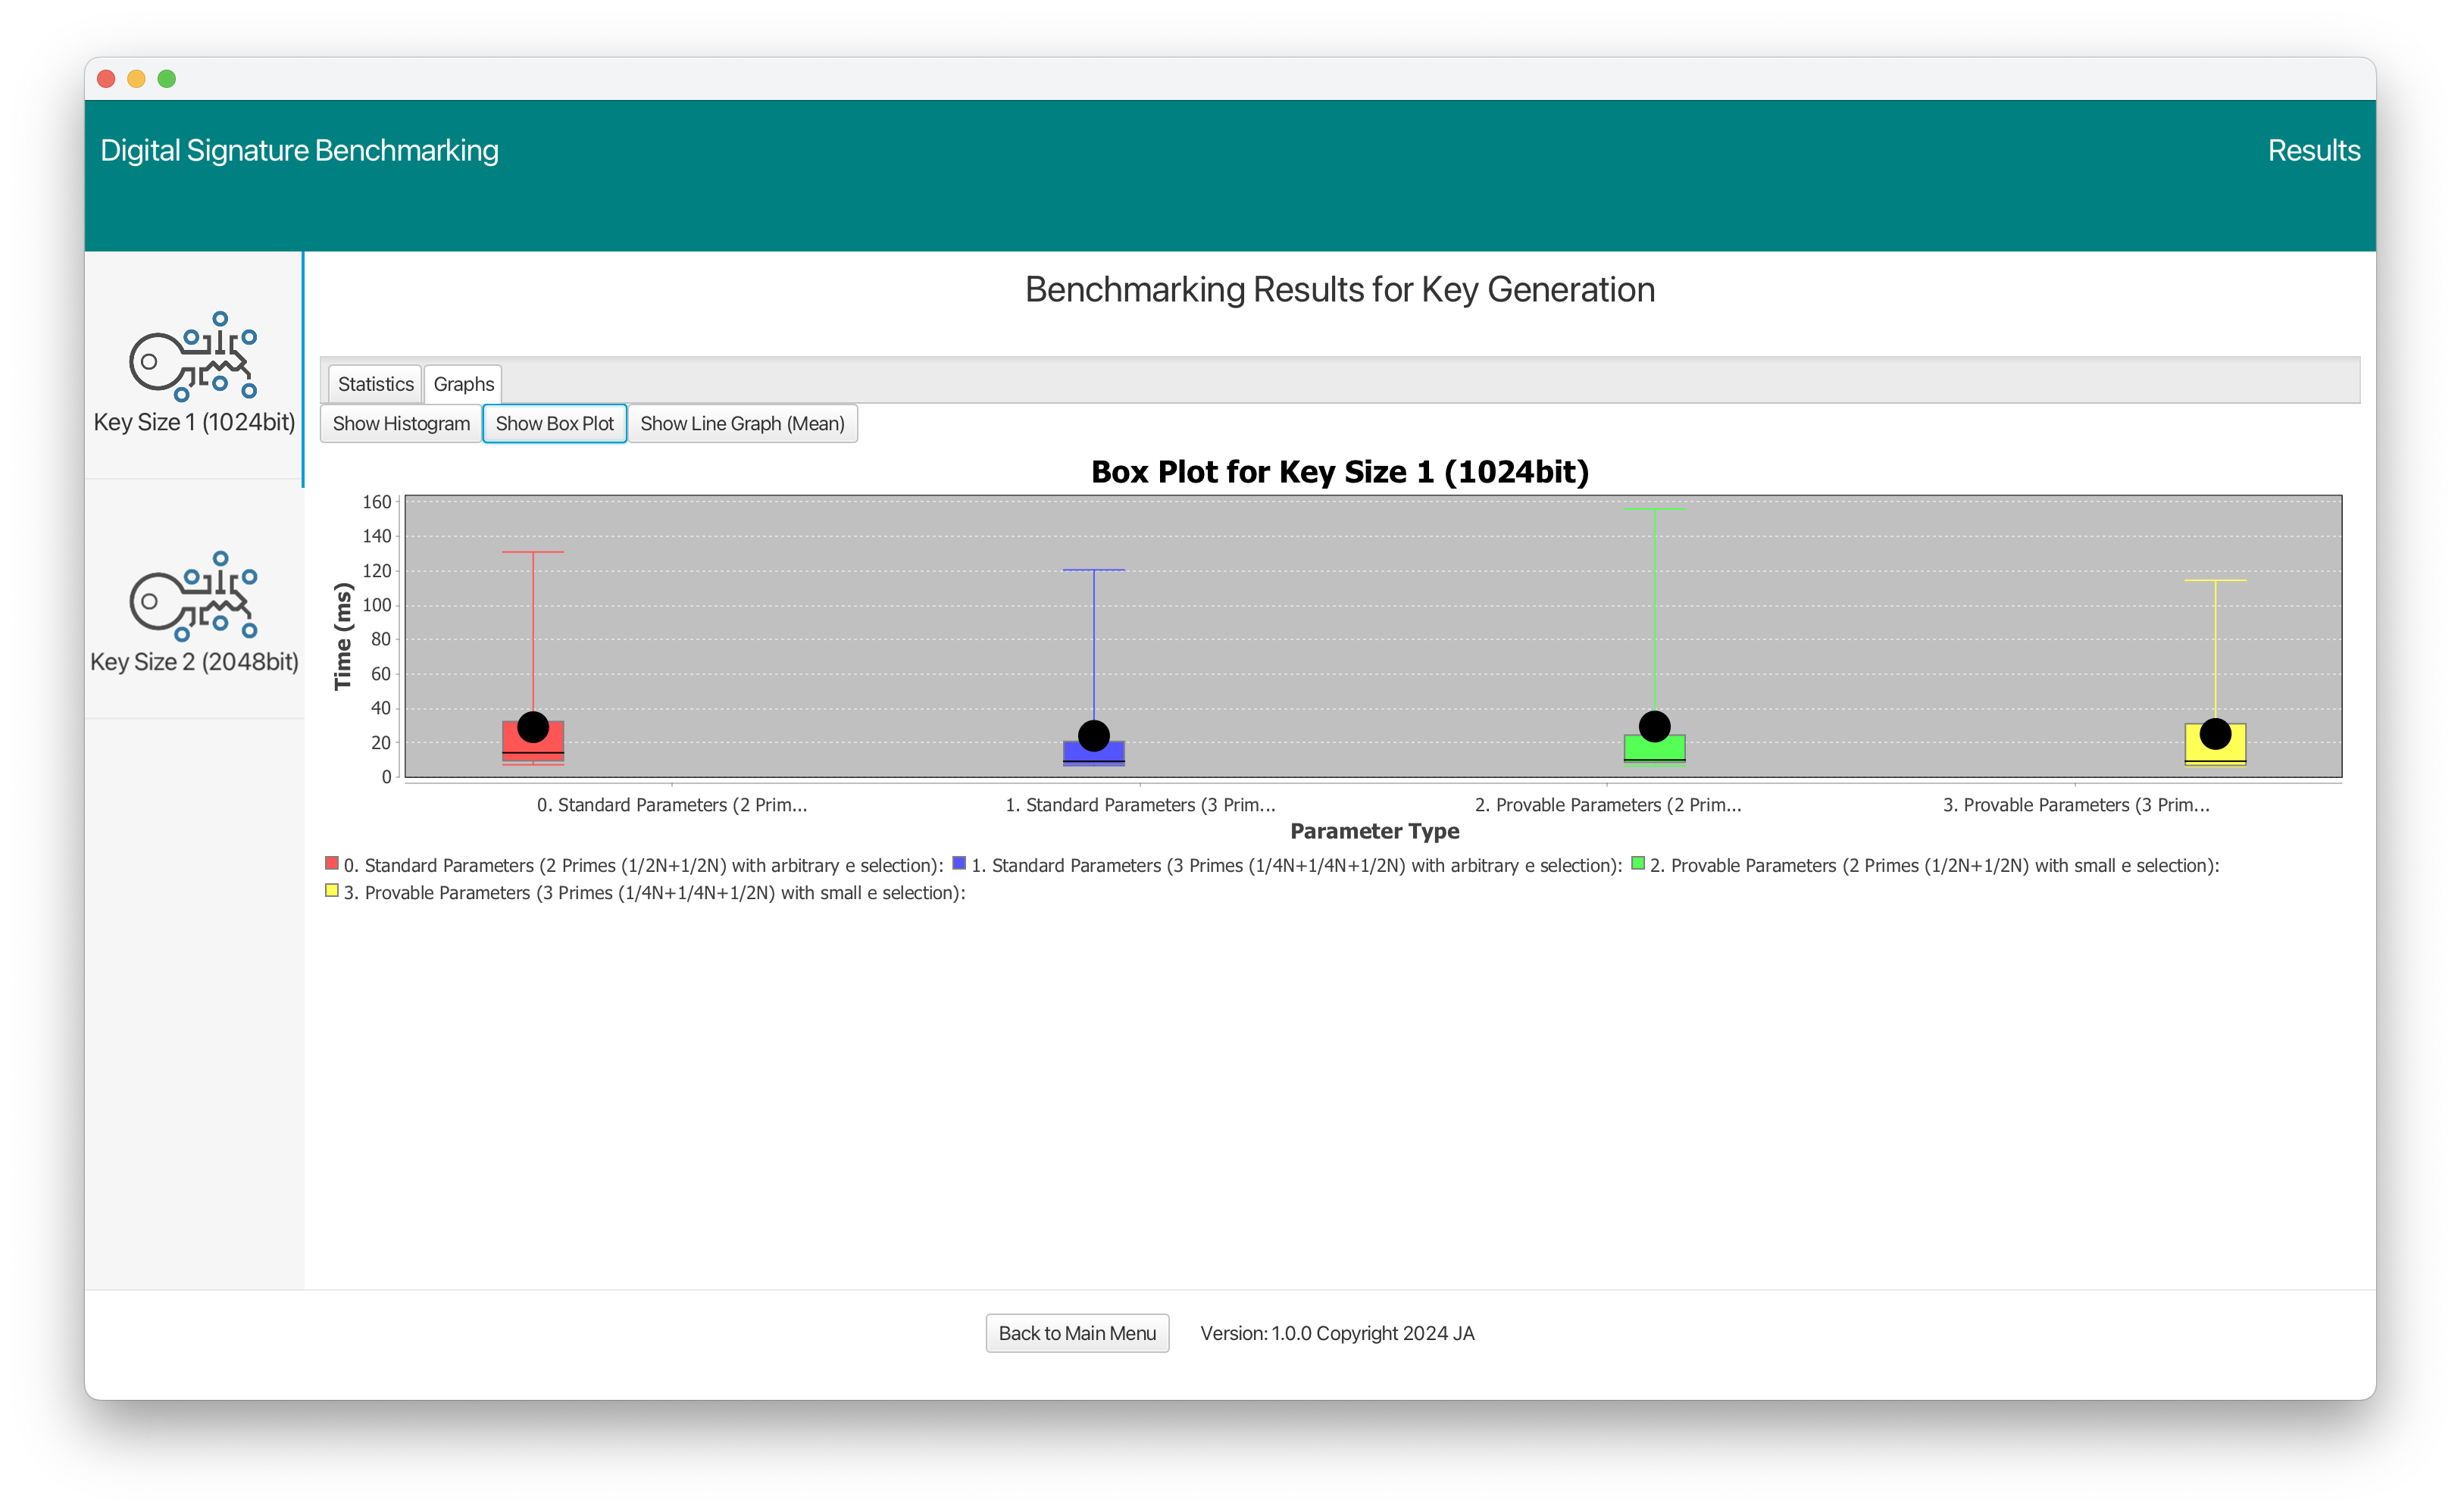
\includegraphics[width=\textwidth]{main_pictures/ui/keyGen/keyGen6.png}} % Adding border here
       \caption{Comparison Benchmarking: Key Generation: Overlaid Box plot graph}
        \label{fig:image2}
    \end{minipage}
     \begin{minipage}{0.7\textwidth}
        \centering
        \fbox{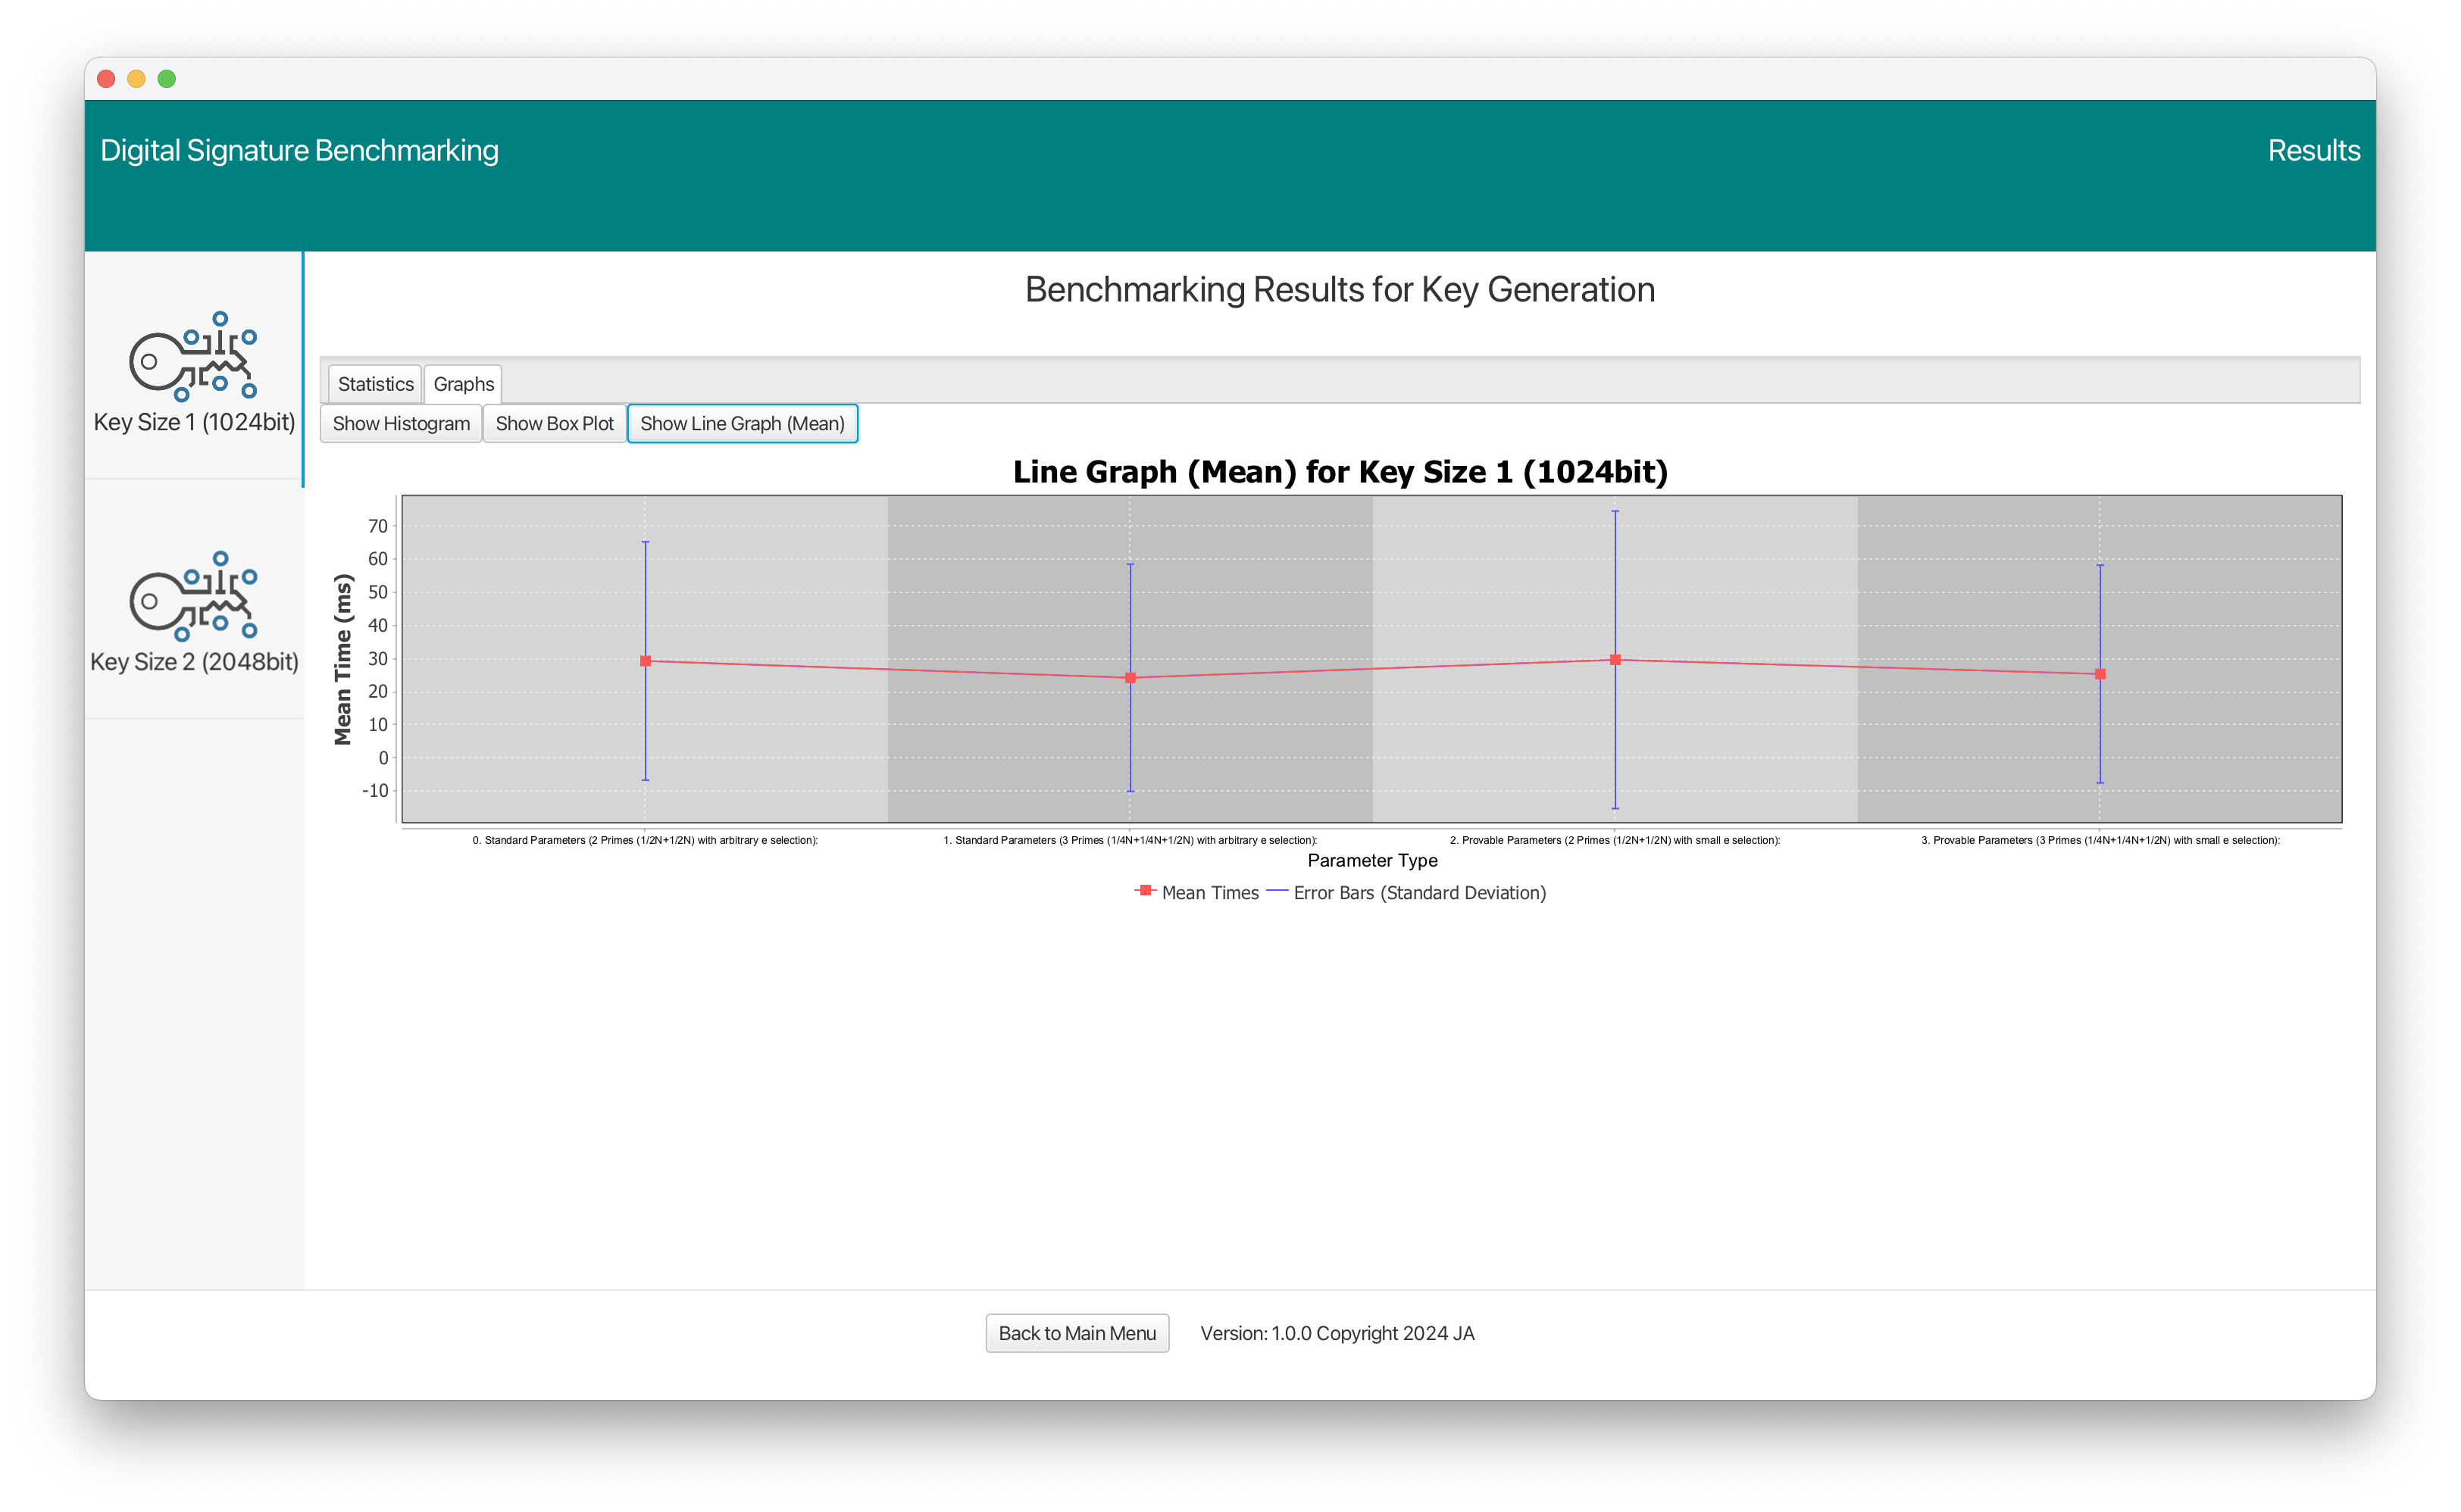
\includegraphics[width=\textwidth]{main_pictures/ui/keyGen/keyGen7.png}} % Adding border here
       \caption{Comparison Benchmarking: Key Generation: Overlaid Line graph for mean times}
        \label{fig:image2}
    \end{minipage}
\end{figure}
An alternative graphical representation of the results can be accessed by navigating to the "Graphs" tab within the central tab pane, where the results table is situated. This tab offers support for three distinct types of graphs, each containing data from all key configurations mapped from the table for easy comparison. These graph types include a stacked histogram, which visualises the distribution of results among configurations for each key size. Additionally, box plots are provided for inferring the distribution of data among configurations. Lastly, mean time line graphs (with error bars for standard deviation) facilitate comparison of average performance and variability among configurations.

\subsection{Signature Generation}
\begin{figure}[H]
    \centering
    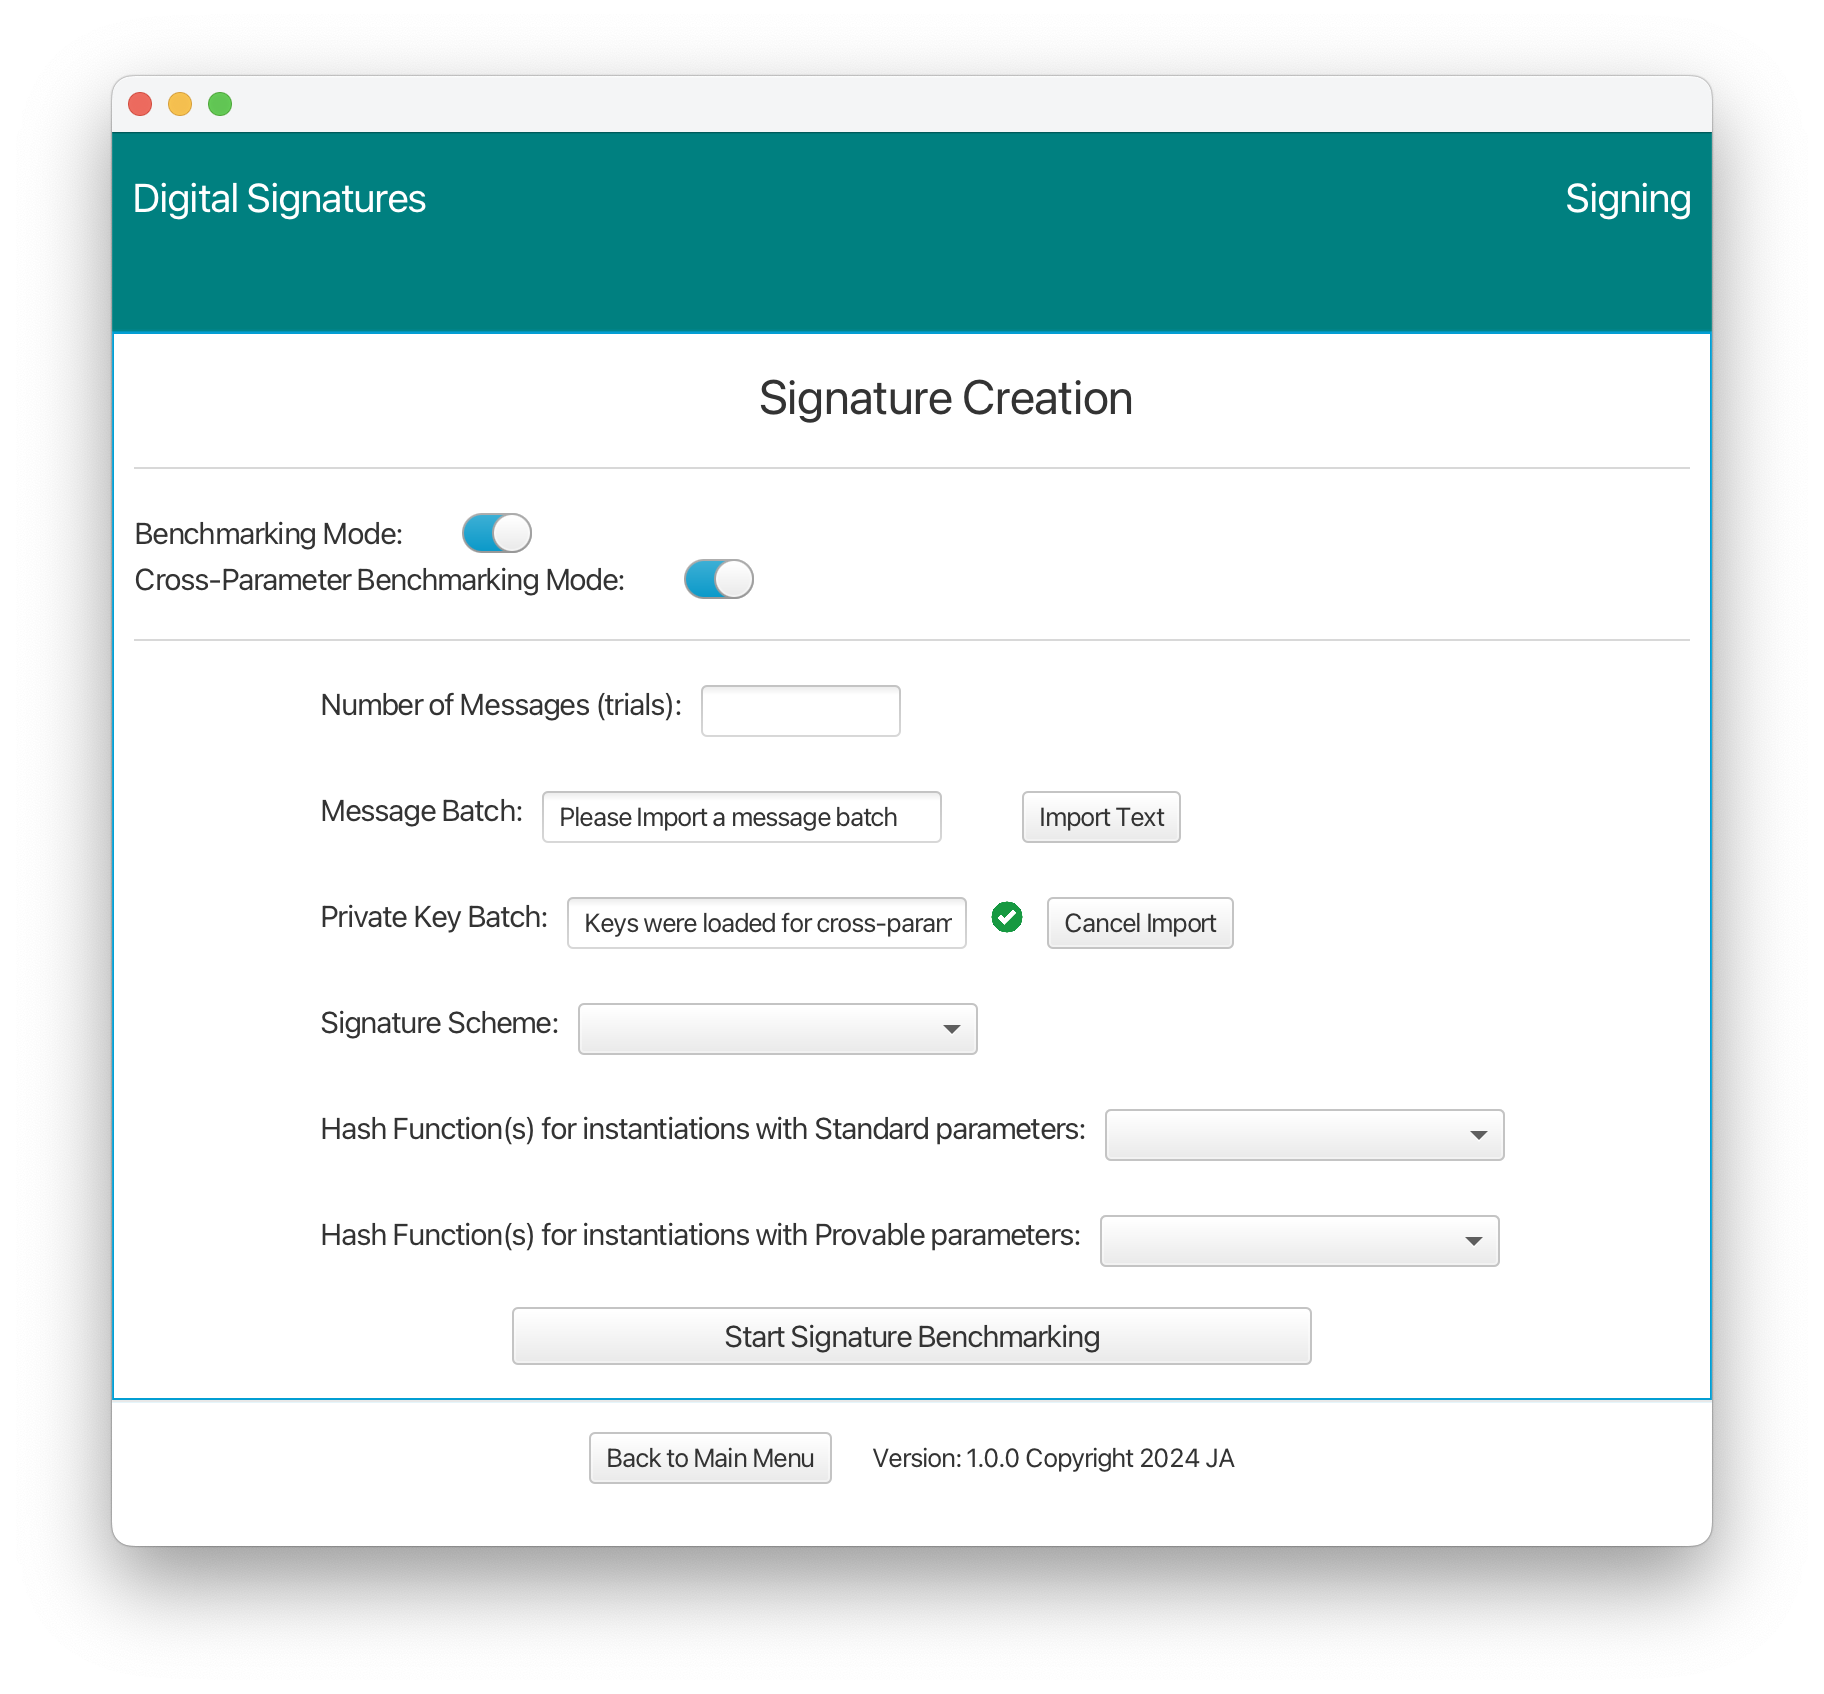
\includegraphics[scale= 0.4]{main_pictures/ui/signing/signing1.png}
   \caption{Comparison Benchmarking: Signature Generation (Comparison Benchmarking)}
\end{figure}
The initial signature generation screen for comparison benchmarking is activated by completing a key generation benchmarking run in comparison mode. On completion of this, the private key batch (which is also available for export from the results table tab) is preloaded into the signature creation portal. Thus when signature generation option is selected from the main menu, the comparison benchmarking screen is displayed rather than the default benchmarking screen.
This explains the state of cross-parameter benchmarking toggle being set as switched on, as well as, specialised options appearing such as the application displaying a visual indication that a comparison-compatible private key batch was preloaded.



\begin{figure}[H]
    \centering % Center the images
    
    % First image in a minipage
    \begin{minipage}{0.4\textwidth}
        \centering
        \fbox{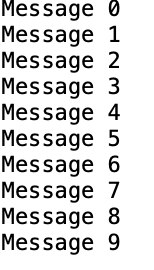
\includegraphics[width=0.4\textwidth]{main_pictures/ui/signing/signing2.png}} % Adding border here
       \caption{Comparison Benchmarking: Signature Creation (Test message batch (testMessages.txt))}
        \label{fig:image1}
    \end{minipage}
    \hfill % Add some space between the images
    % Second image in a minipage
    \begin{minipage}{0.58\textwidth}
        \centering
        \fbox{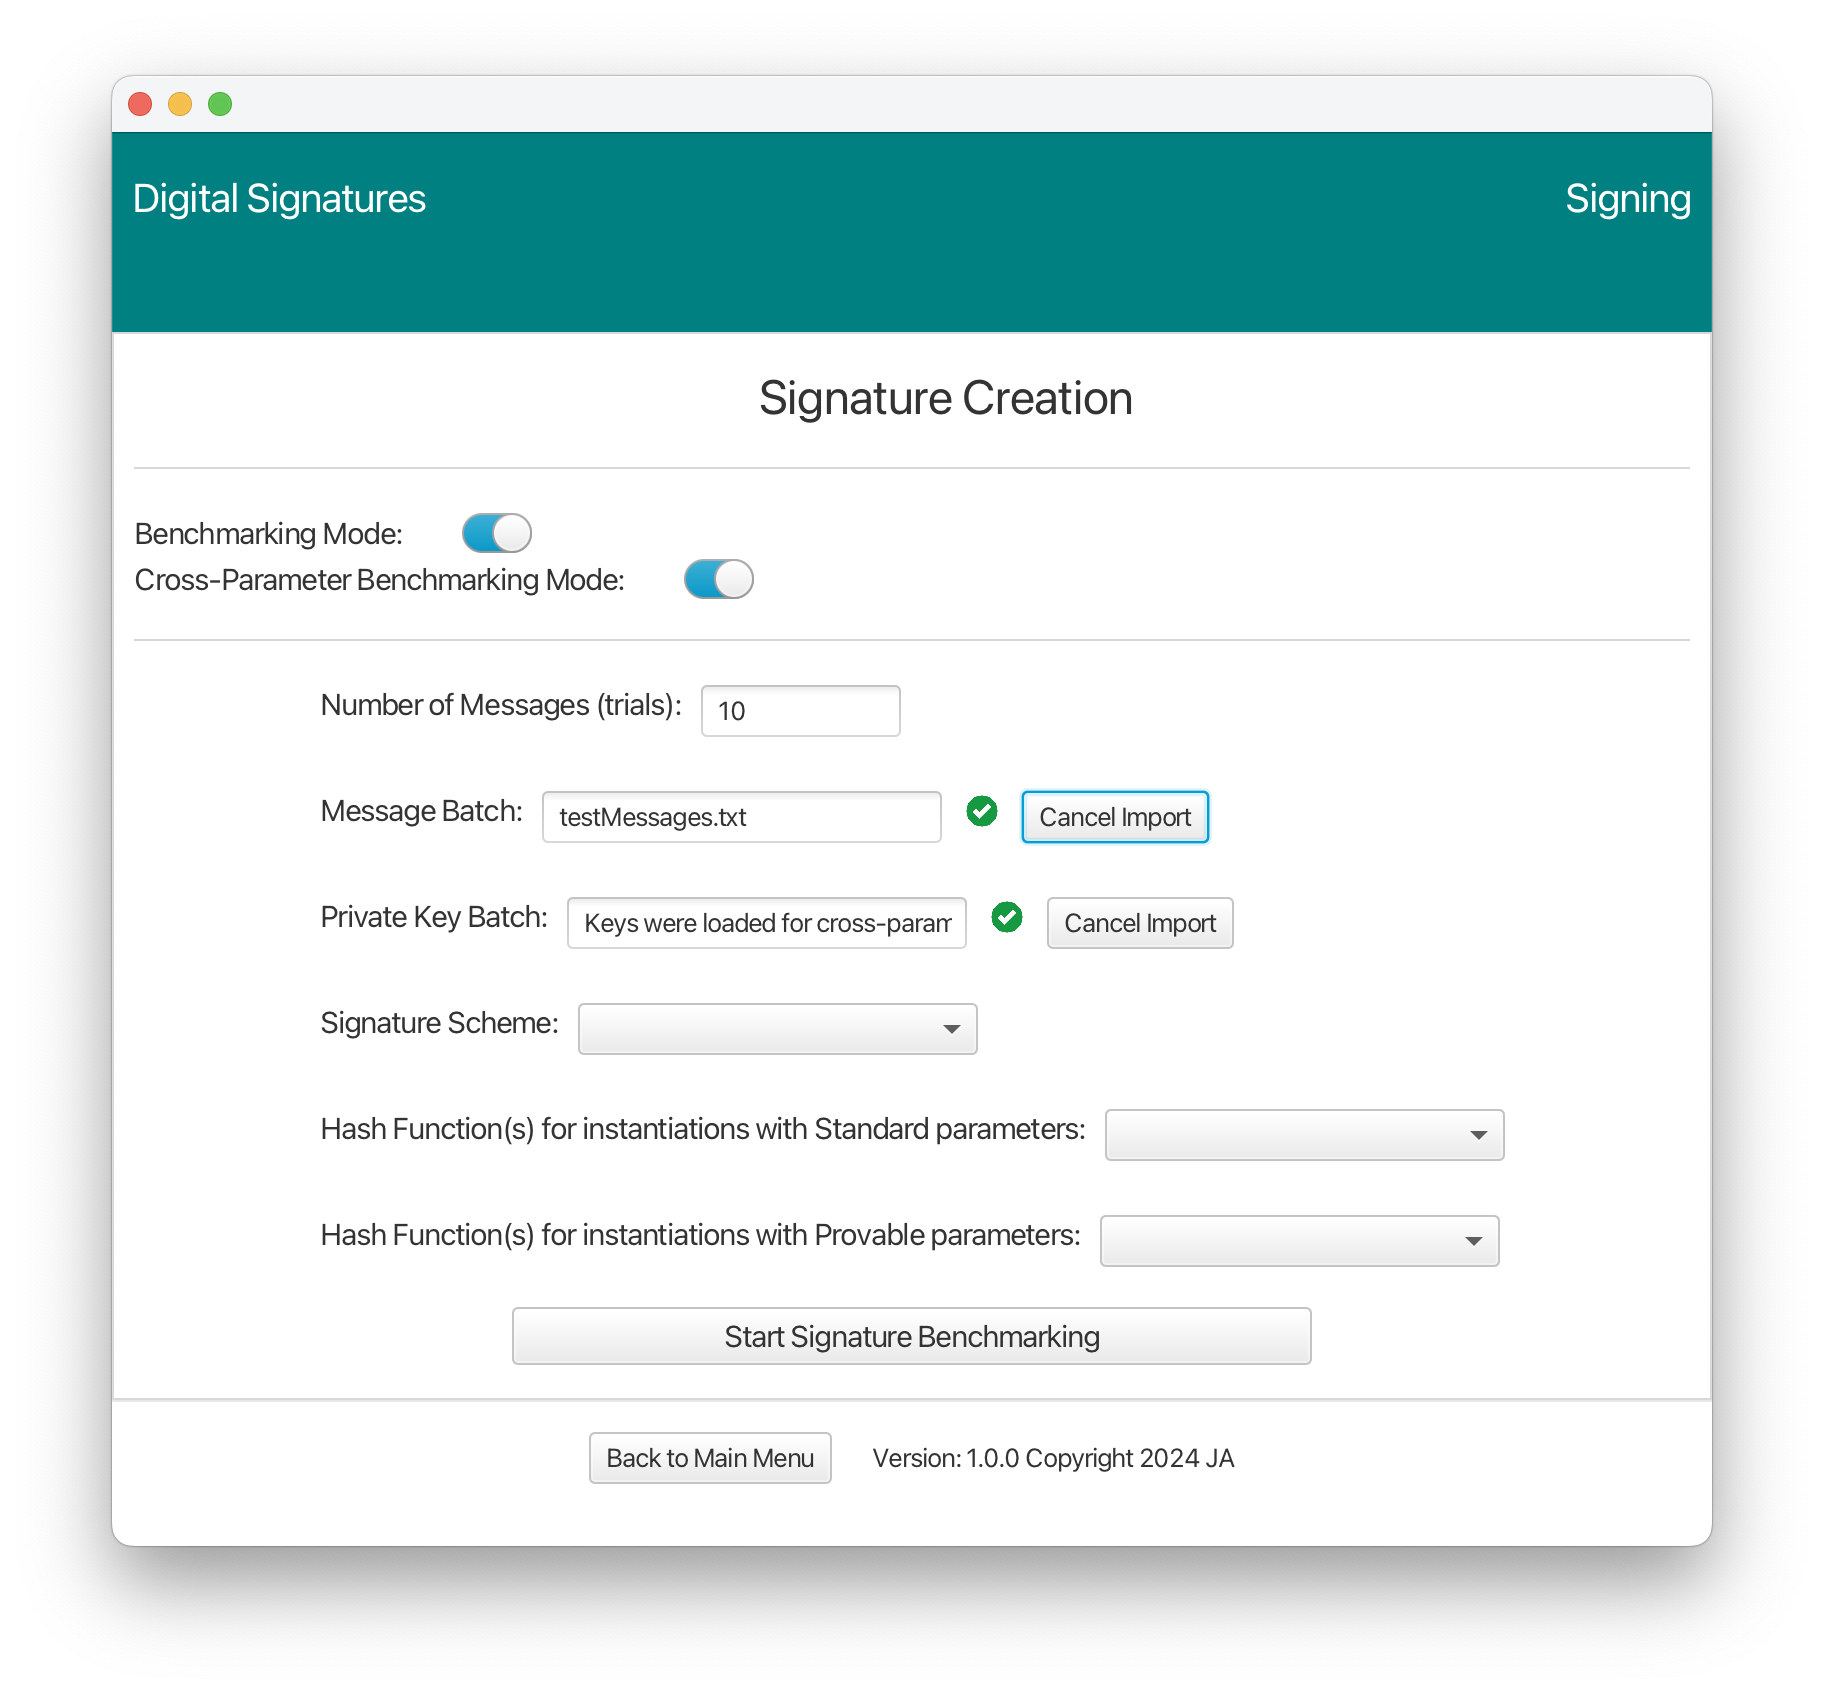
\includegraphics[width=\textwidth]{main_pictures/ui/signing/signing3.png}} % Adding border here
       \caption{Comparison Benchmarking: Signature Creation (Imported message batch)}
        \label{fig:image2}
    \end{minipage}
\end{figure}


The signature creation screen is first organised with a pair of fields related to the importing of a message batch. There are specific requirements for the import of the message batch. 

The application expects the message batch as a non interrupted and new line separated sequence of messages and the number of lines must match the number entered in the adjacently above field. Otherwise import of a message batch is prevented.

On successful validation, the screen is updated with a checkmark indicator that provides visual confirmation that the message batch was successfully imported. The interface also includes a dropdown menu labeled signature scheme giving users the option to select the desired signature scheme  to be applied. 

\begin{figure}[H]
    \centering % Center the images
    
    % First image in a minipage
    \begin{minipage}{0.49\textwidth}
        \centering
        \fbox{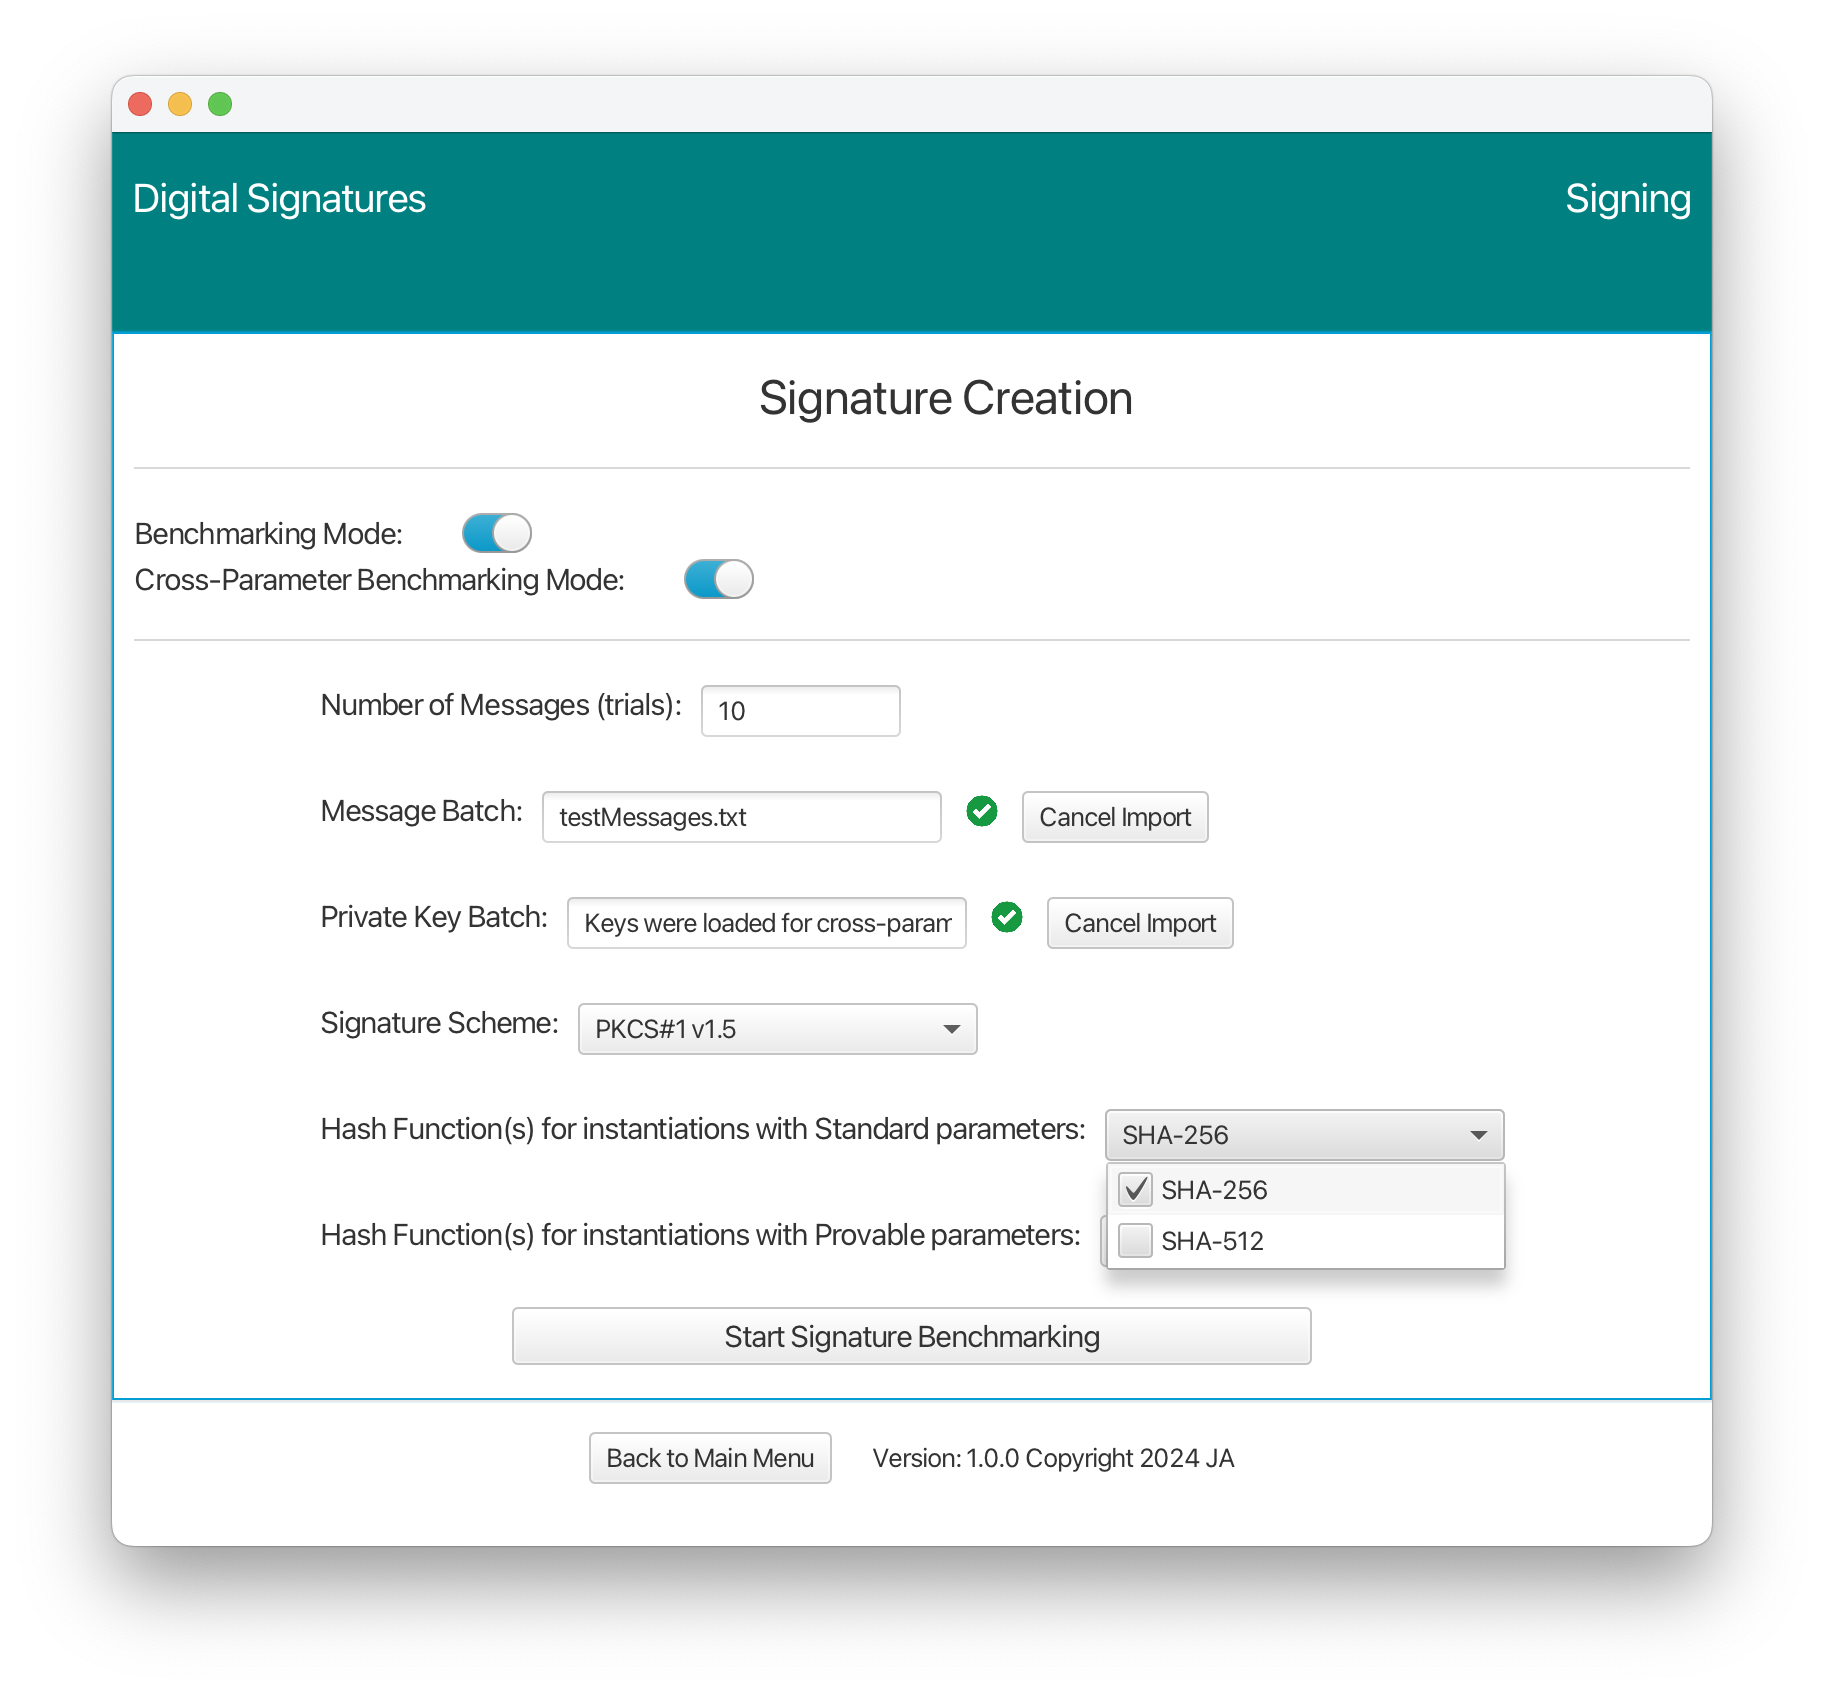
\includegraphics[width=\textwidth]{main_pictures/ui/signing/signing4.png}} % Adding border here
       \caption{Comparison Benchmarking: Signature Creation (Standard Parameter Hash Functions)}
        \label{fig:image1}
    \end{minipage}
    \hfill % Add some space between the images
    % Second image in a minipage
    \begin{minipage}{0.49\textwidth}
        \centering
        \fbox{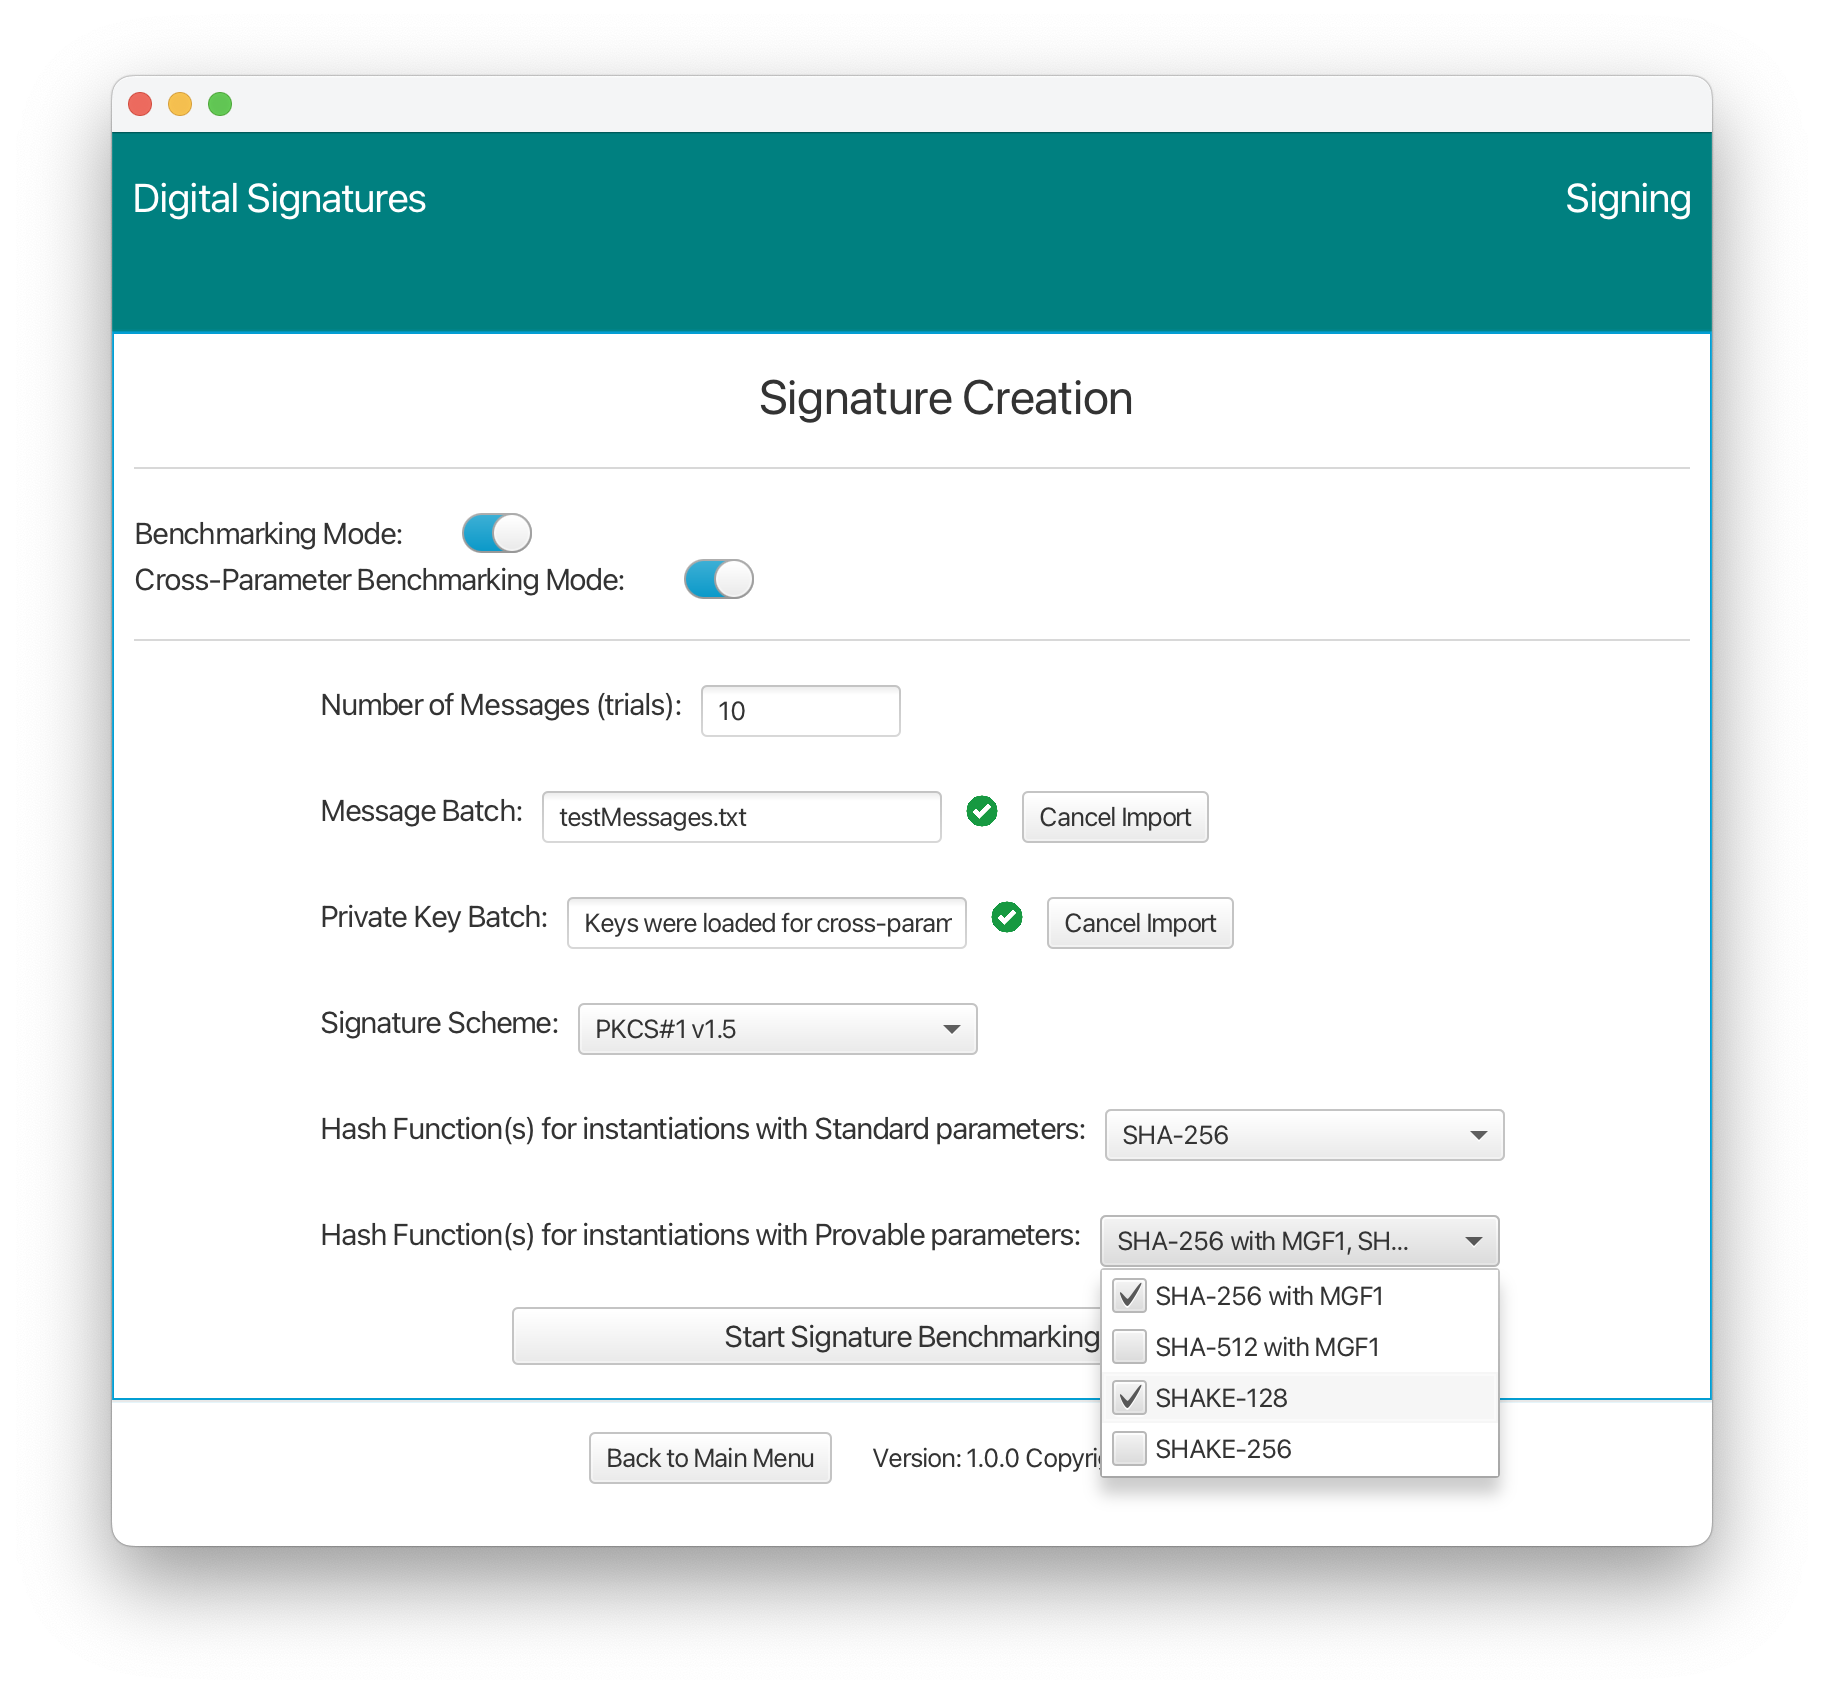
\includegraphics[width=\textwidth]{main_pictures/ui/signing/signing5.png}} % Adding border here
       \caption{Comparison Benchmarking: Signature Creation (Provably Secure Parameter Hash Functions)}
        \label{fig:image2}
    \end{minipage}
      \begin{minipage}{0.55\textwidth}
        \centering
        \fbox{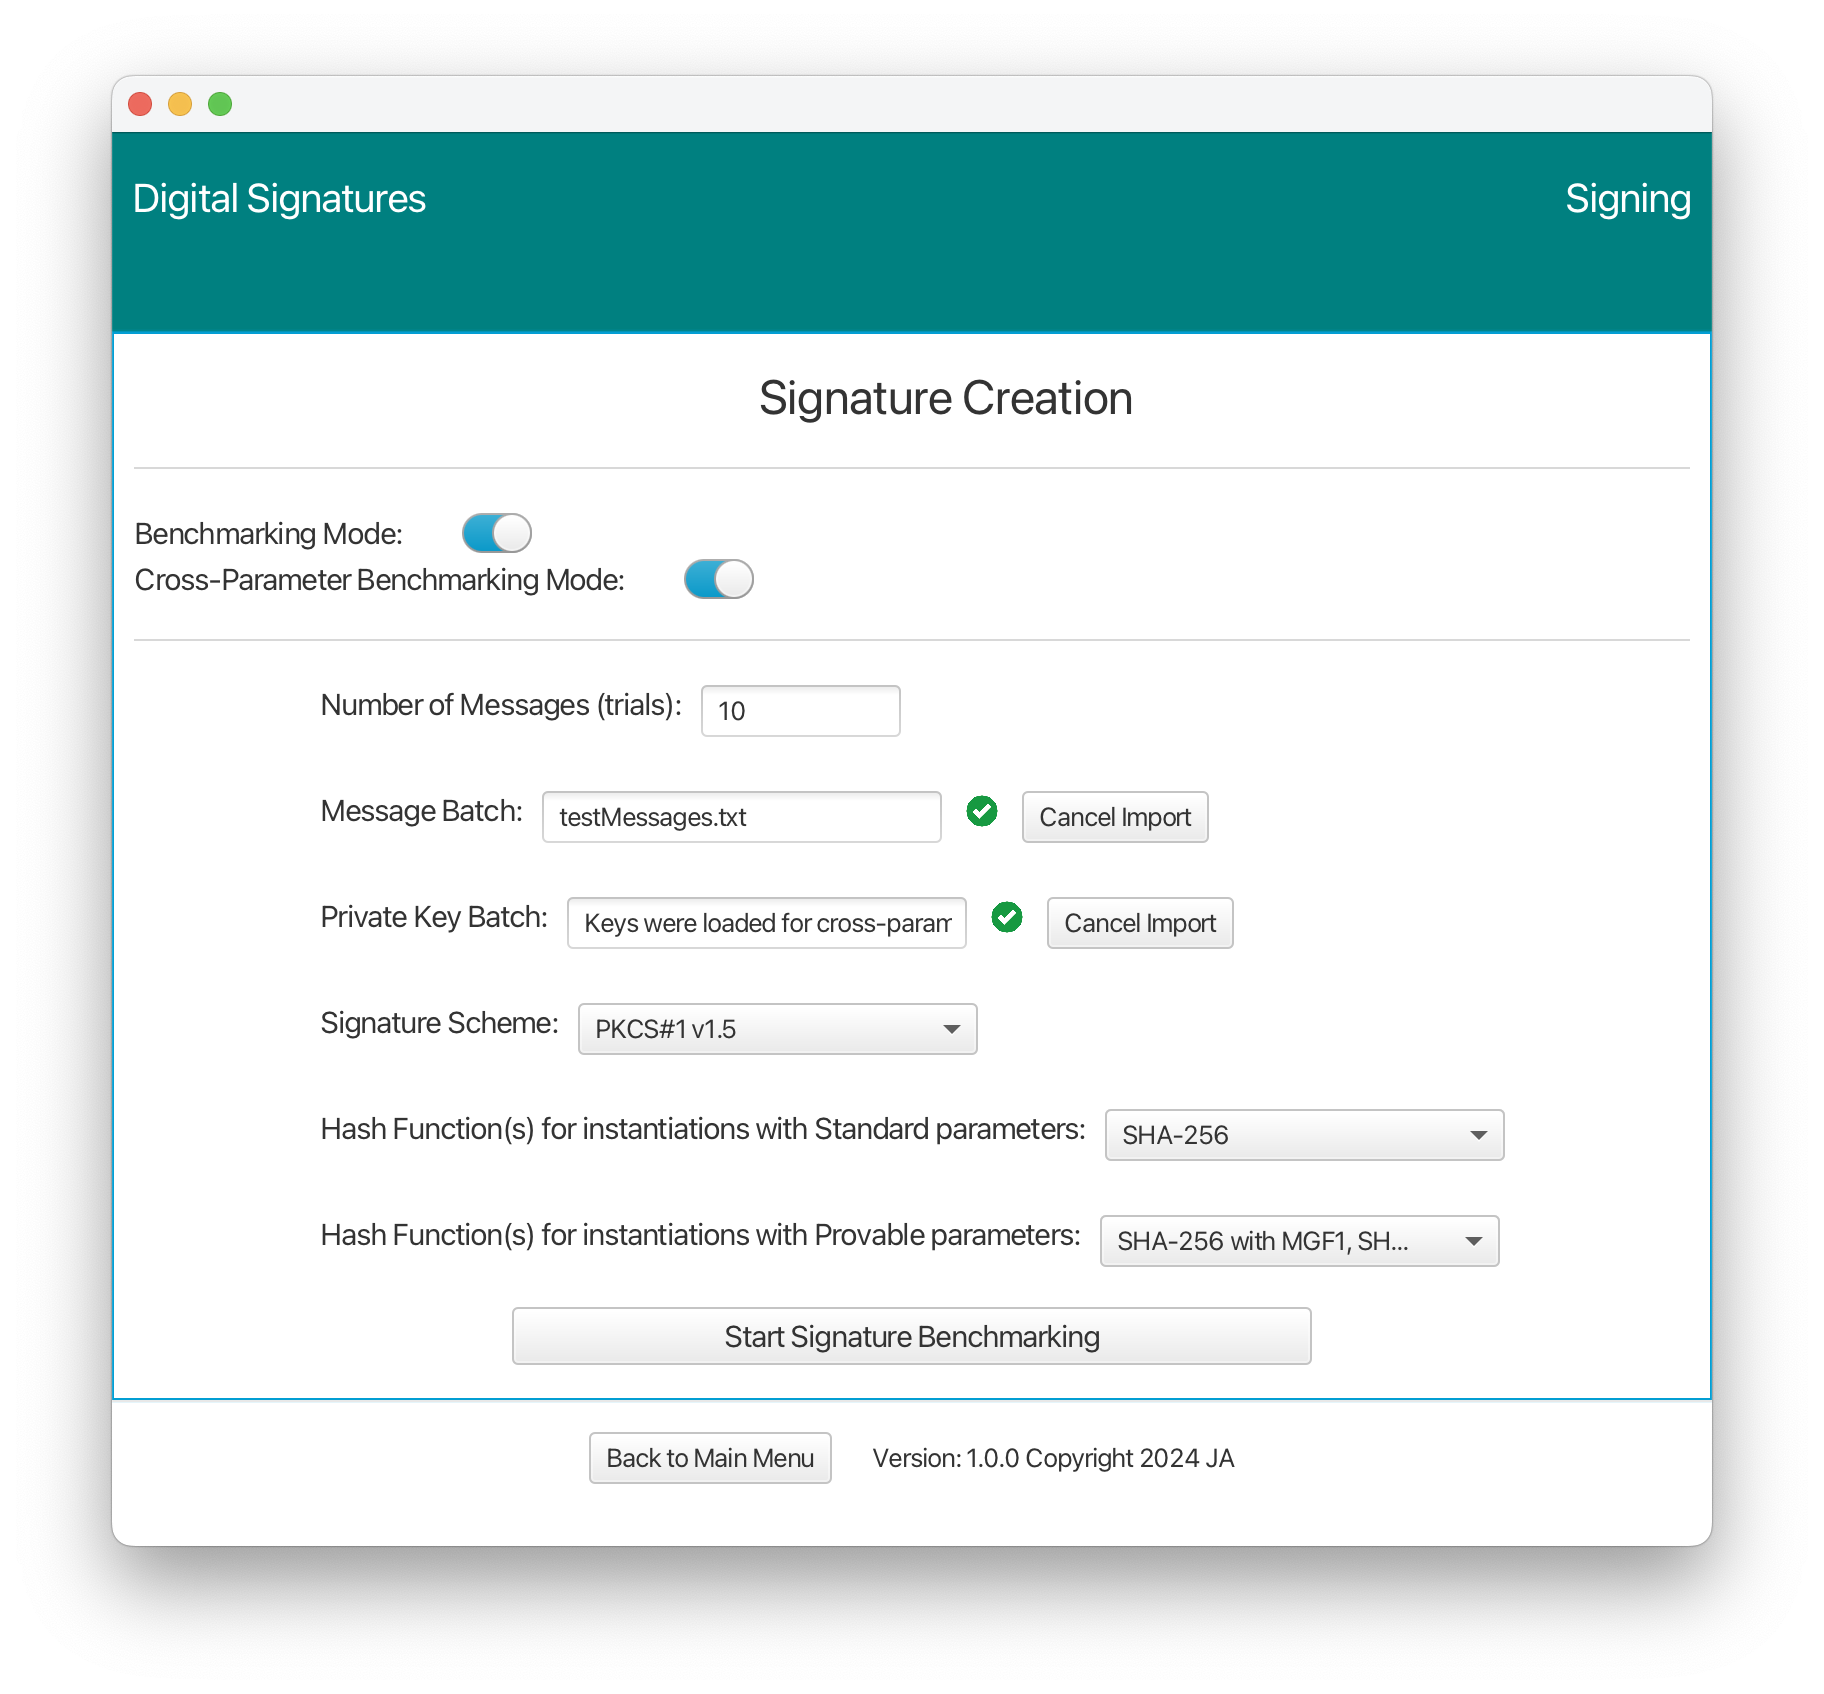
\includegraphics[width=1.2\textwidth]{main_pictures/ui/signing/signing6.png}} % Adding border here
       \caption{Comparison Benchmarking: Signature Creation (All inputs provided)}
        \label{fig:image2}
    \end{minipage}
\end{figure}

In comparison benchmarking mode for signature generation, users select hash functions for standard (fixed-length) and provably secure (variable-length) parameters via a multi-choice drop-down menu. The process involves:

Computing signatures for each selected fixed-length hash function, using the first two key configurations (standard parameters).
Computing signatures for each chosen variable-length hash function, using the last two key configurations (provably secure parameters).This is done sequentially for each key size.

Clicking "Start Signature Benchmarking" button initiates the execution the benchmarking task. This involves the creation of a batch of signatures for the message batch using the designated signature scheme and hash function-key combinations. A progress bar indicates progress in real time.



\textbf{Comparison Benchmarking: Signature Generation Results Screen}

\begin{figure}[H]
    \centering
    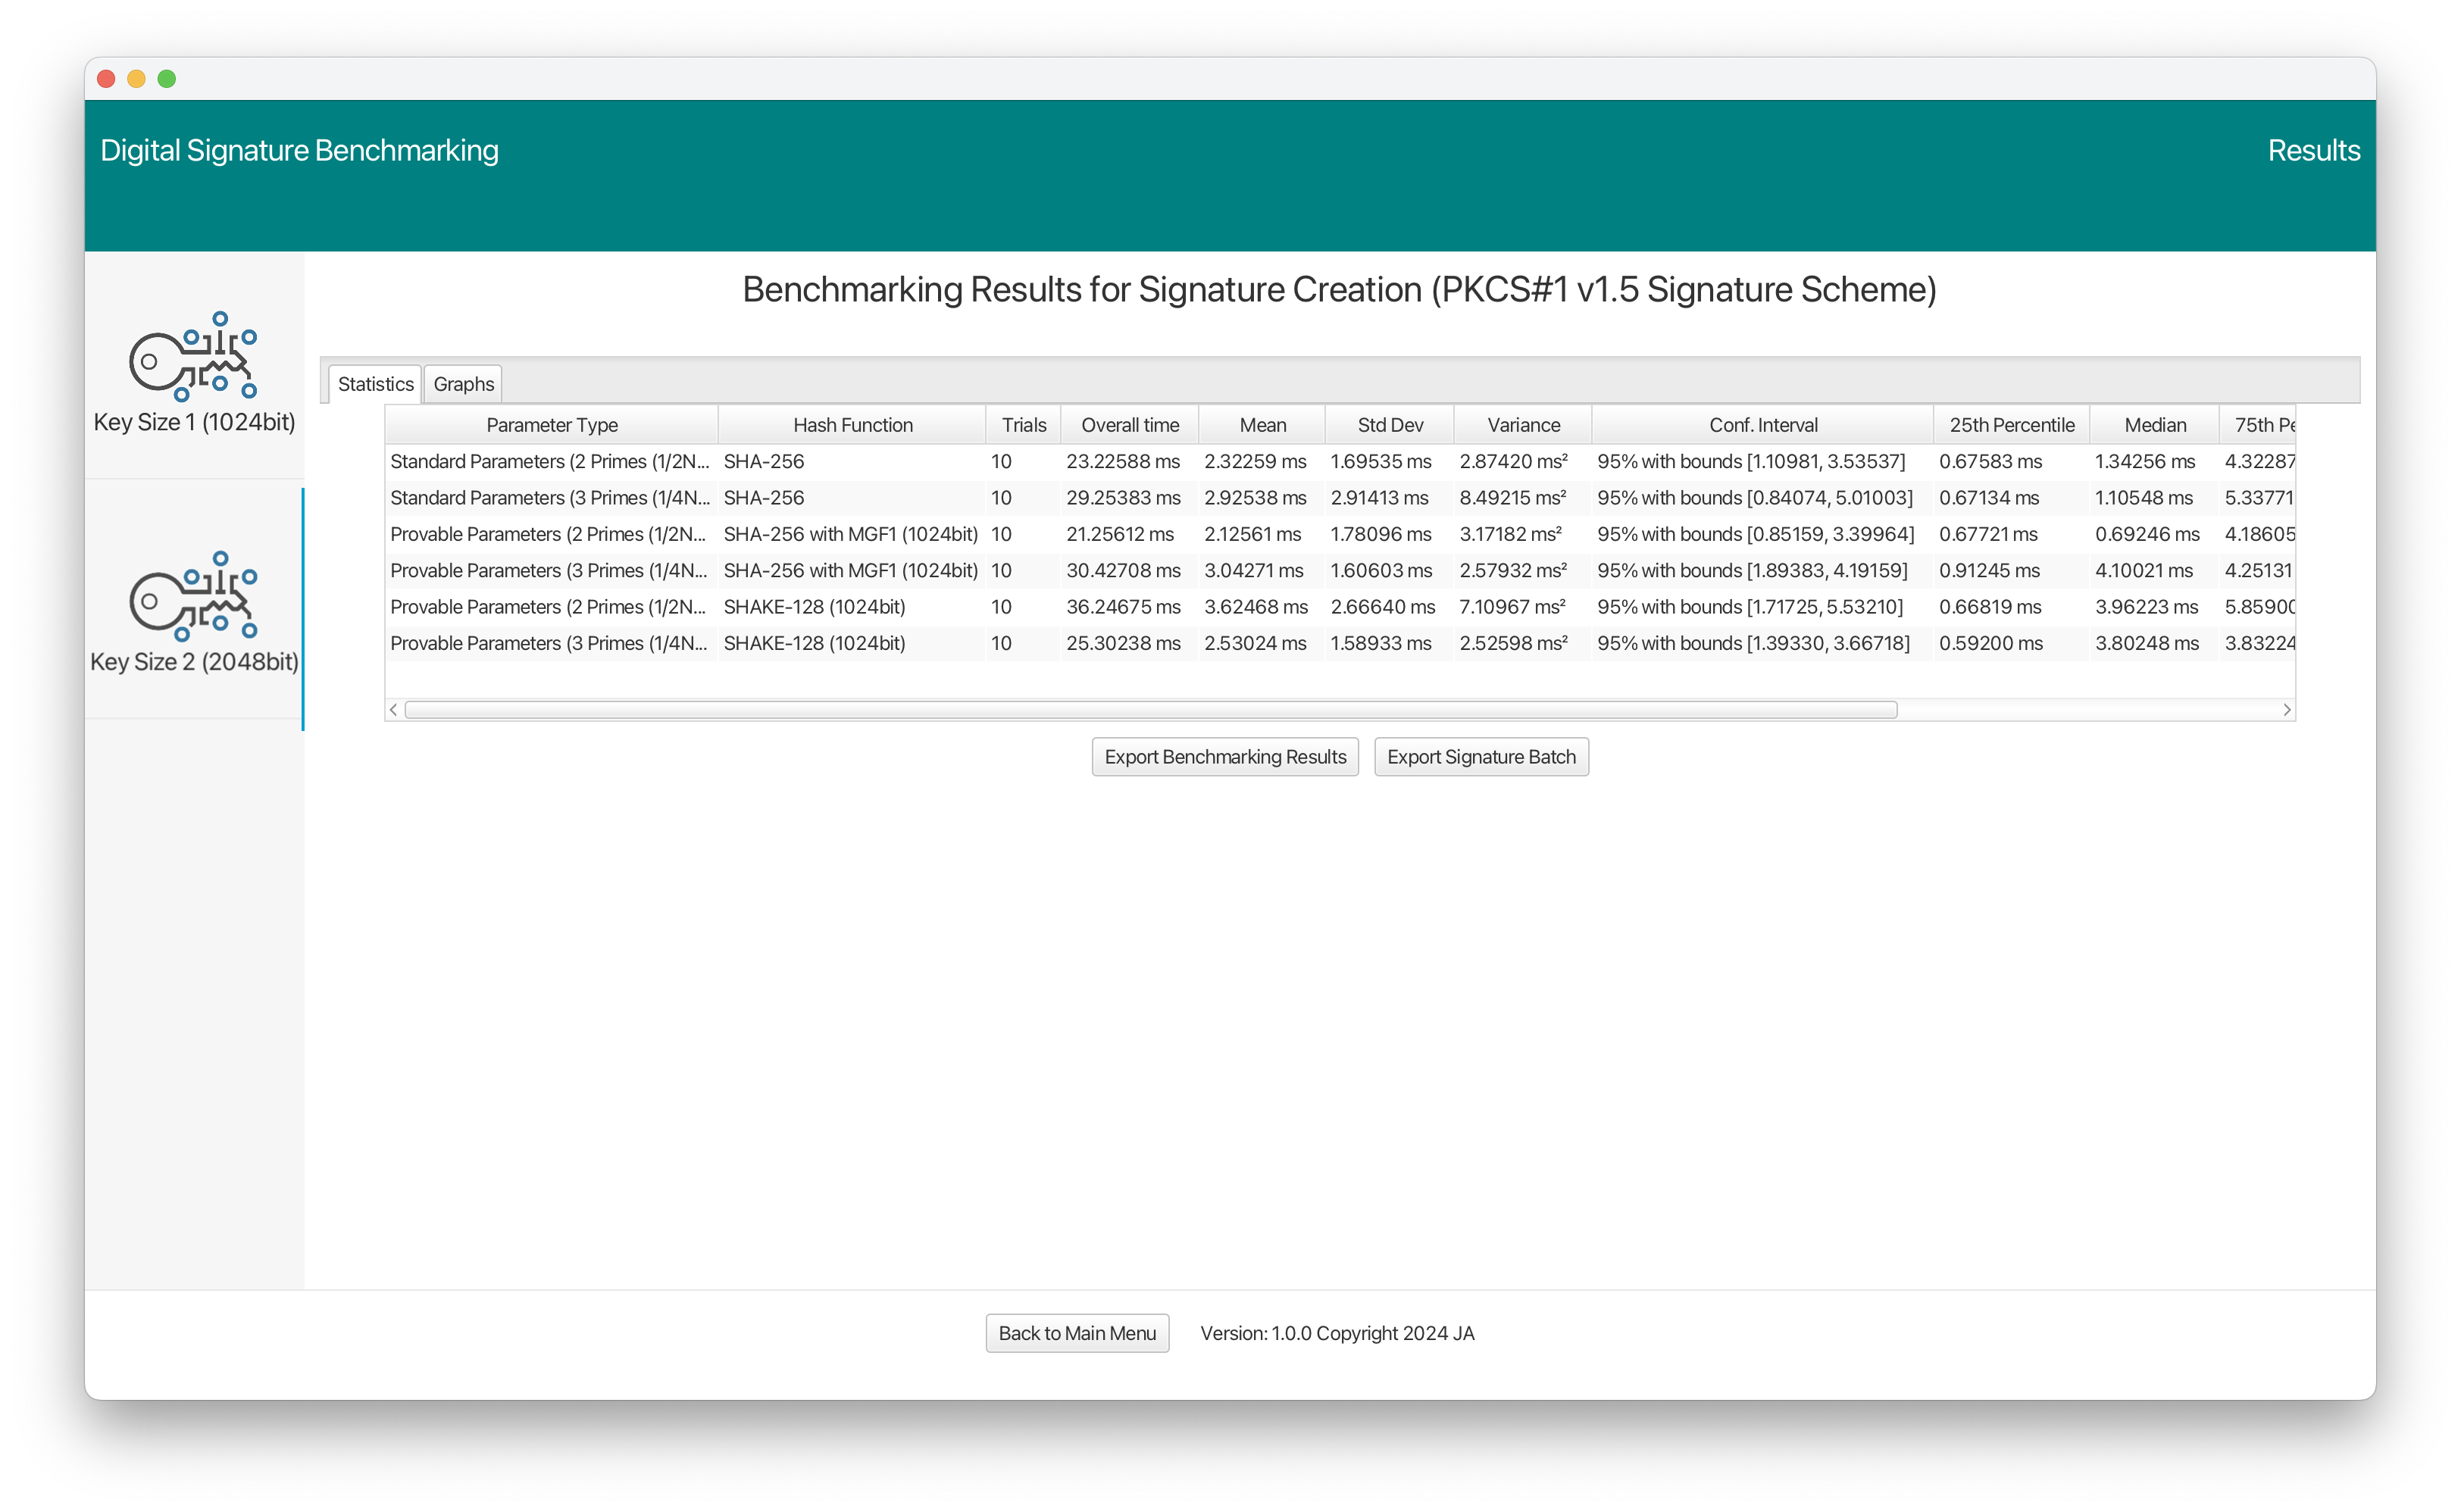
\includegraphics[scale= 0.325]{main_pictures/ui/signing/signing7-2.png}
   \caption{Comparison Benchmarking: Signature Generation (Results Screen)}
\end{figure}

After completing signature generation benchmarking, results from benchmarking are displayed. The results screen features a side pane with tabs for each key size entered. Each tab reveals a results table displaying statistical metrics for all hash function-key combinations.

The table format aligns with the user's hash function choices. For example, selecting one hash function (e.g., SHA-256) for standard parameters results in two rows for this set. For provably secure parameters, if two functions like SHA-256 with MGF1 and SHAKE-128 are chosen, they each generate two rows, totalling four rows. This format leads to six rows per key size, each row representing signature computations for the full message batch.

Below the table, options are available to export benchmarking results and signature batches for each key size. The exported signature batch aligns with the key configurations and hash function combinations used, covering all key sizes in a single file.

\textbf{Comparison Benchmarking: Signature Generation Results Screen Graphs}

\begin{figure}[H]
    \centering % Center the images
    
    % First image in a minipage
    \begin{minipage}{0.7\textwidth}
        \centering
        \fbox{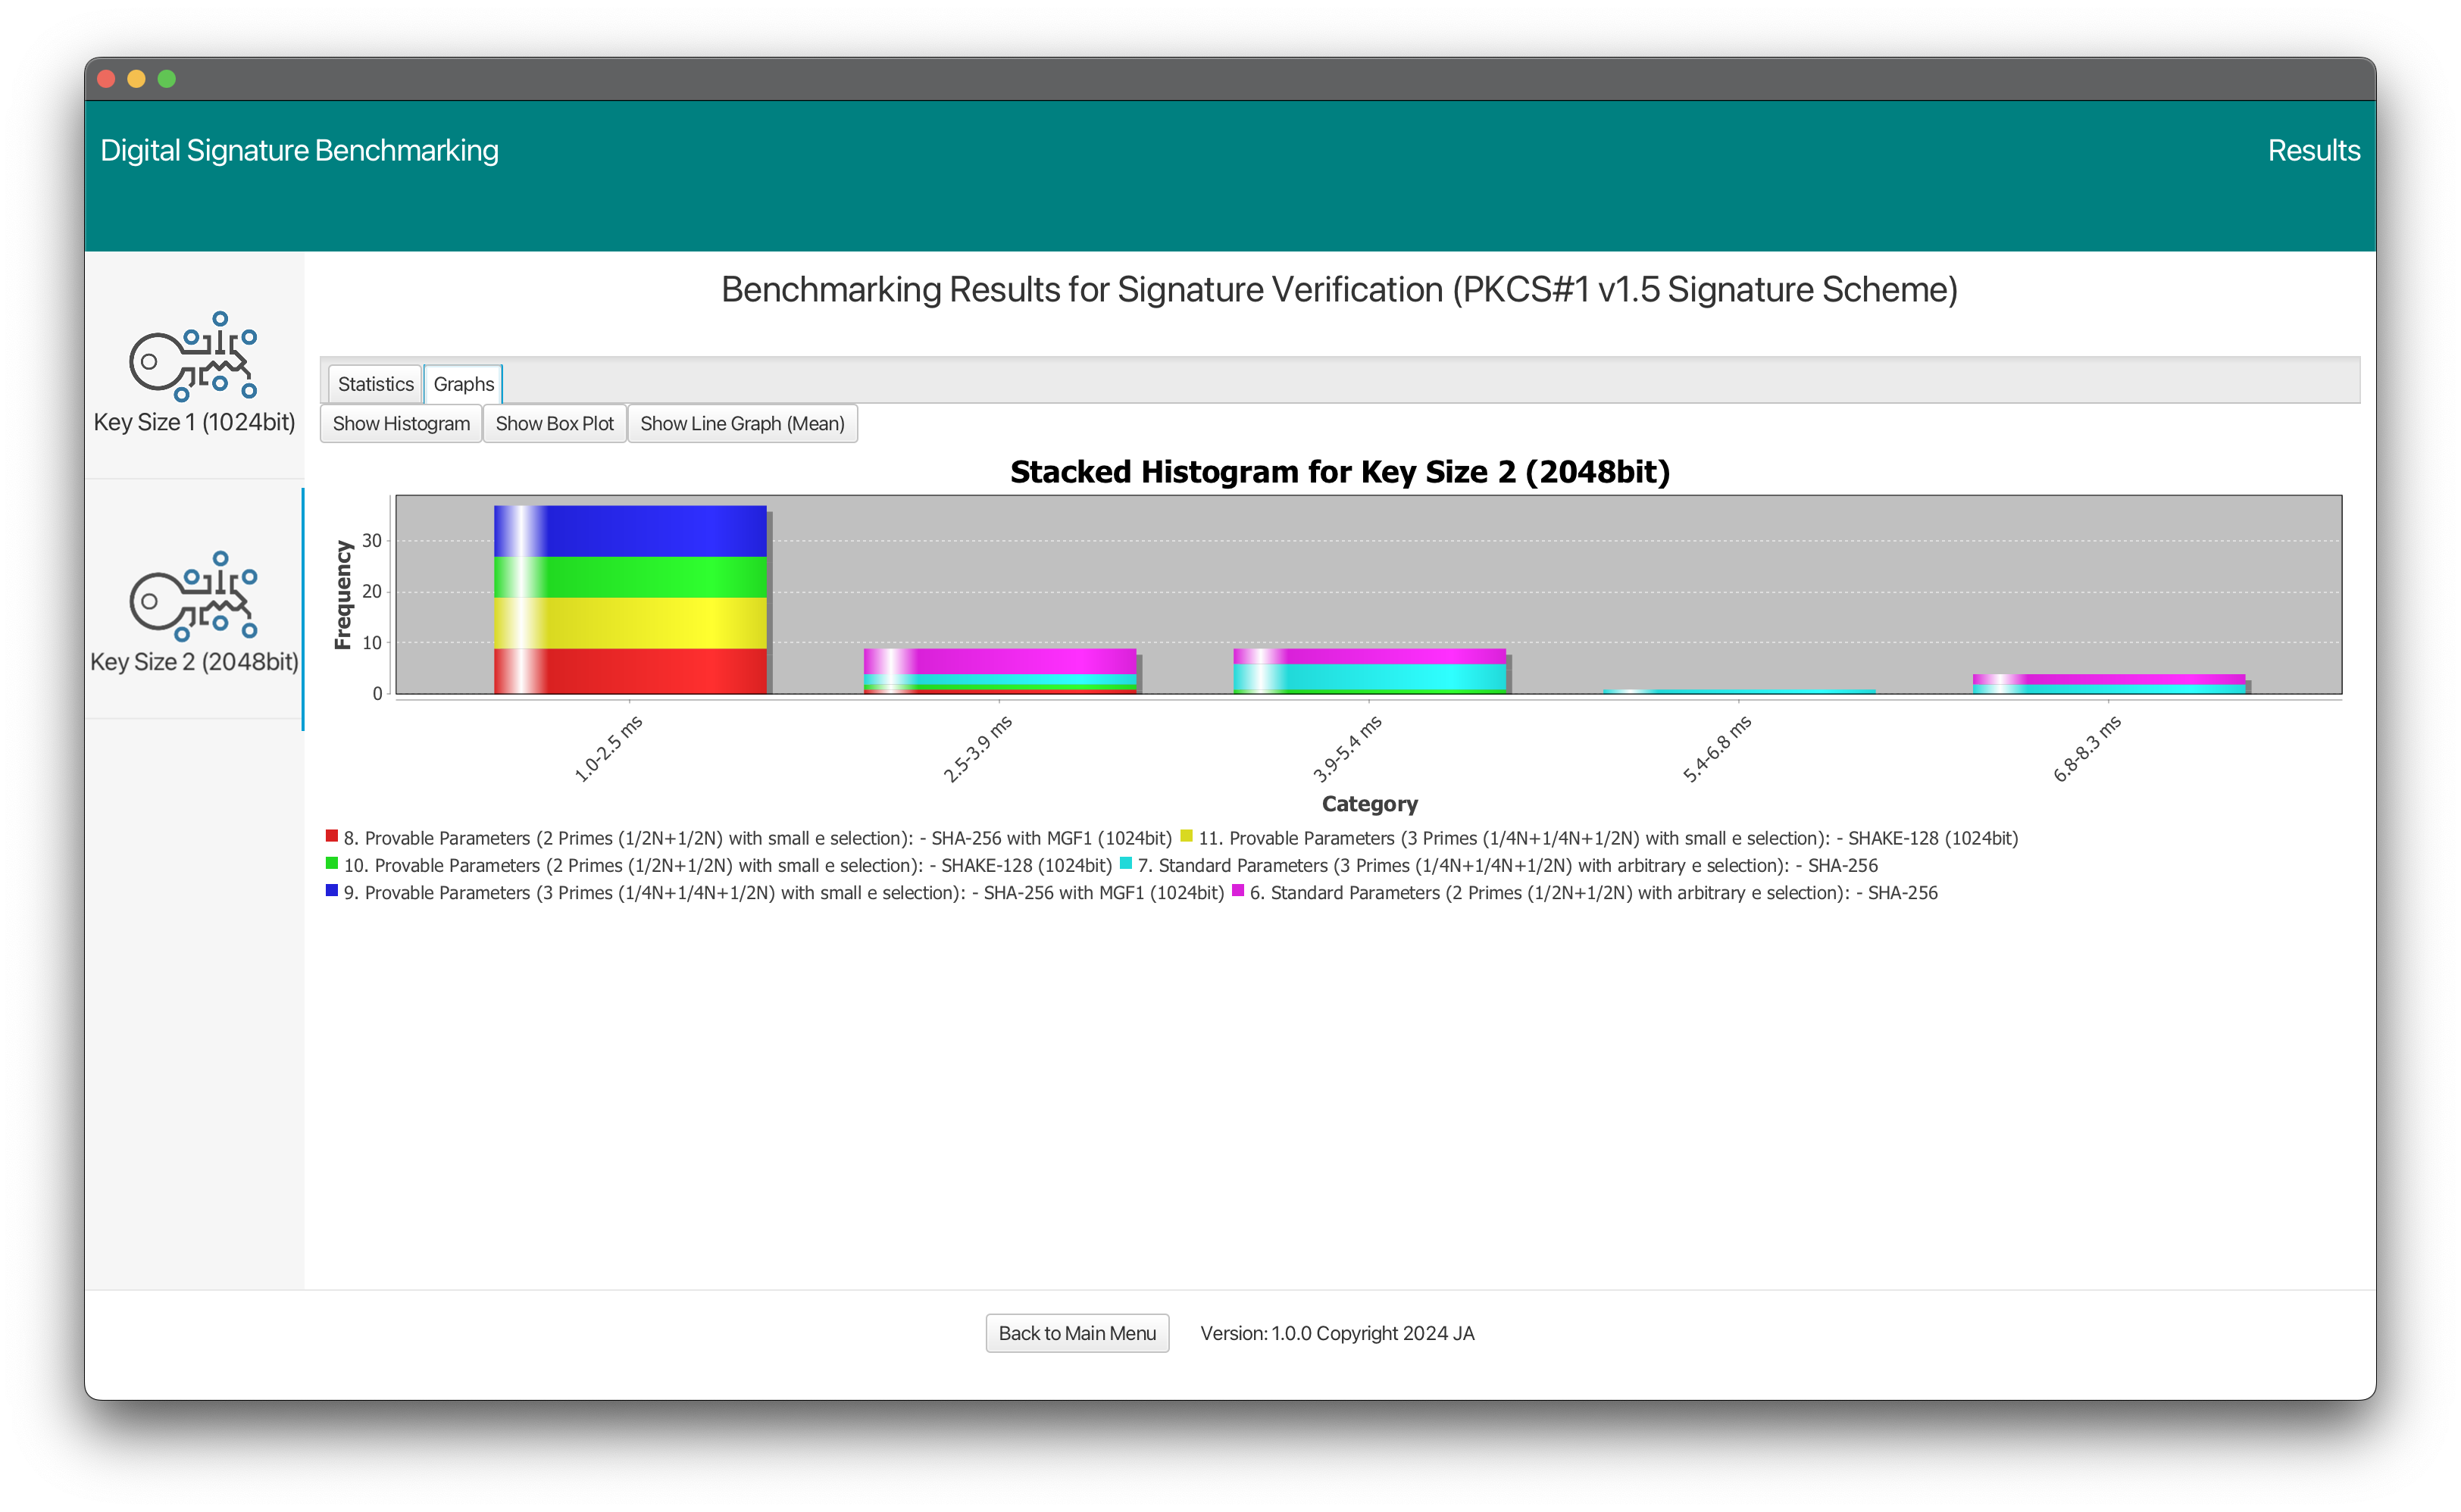
\includegraphics[width=\textwidth]{main_pictures/ui/signing/signing8-2.png}} % Adding border here
       \caption{Comparison Benchmarking: Signature Generation: Overlaid Histogram}
        \label{fig:image1}
    \end{minipage}
    \hfill % Add some space between the images
    % Second image in a minipage
    \begin{minipage}{0.7\textwidth}
        \centering
        \fbox{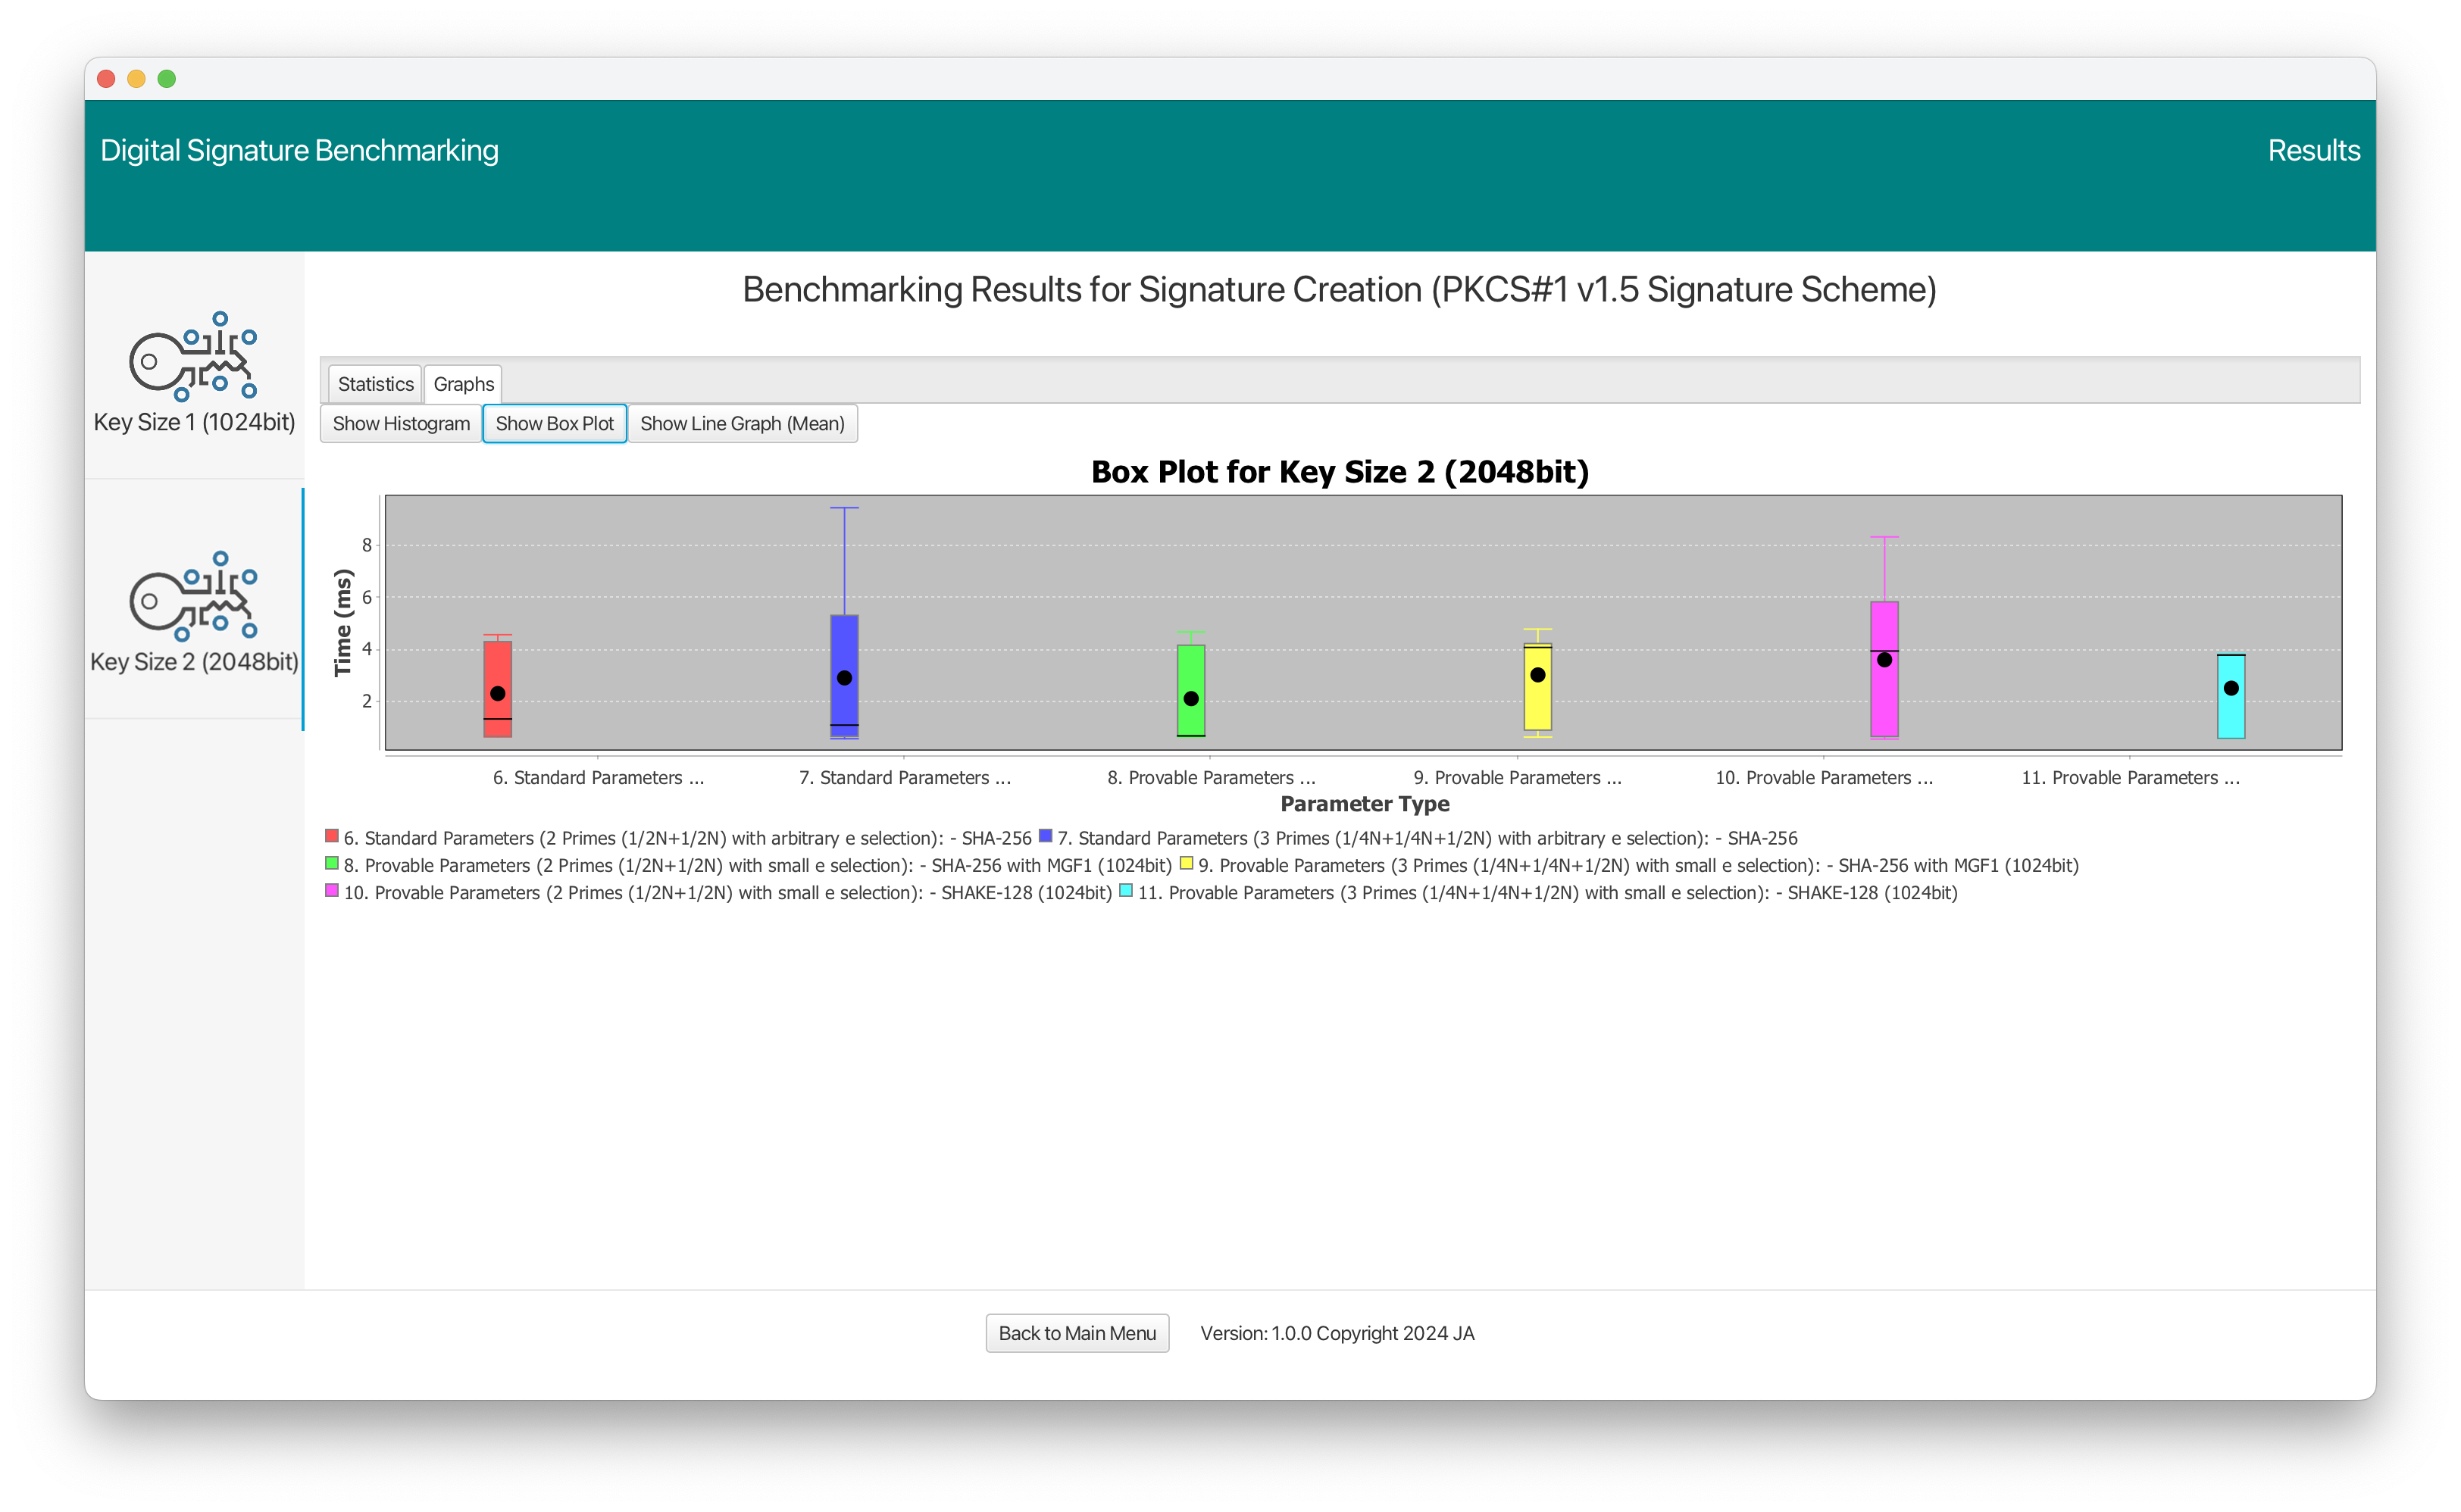
\includegraphics[width=\textwidth]{main_pictures/ui/signing/signing9-2.png}} % Adding border here
       \caption{Comparison Benchmarking: Signature Generation: Overlaid Box plot graph}
        \label{fig:image2}
    \end{minipage}
        \begin{minipage}{0.7\textwidth}
        \centering
        \fbox{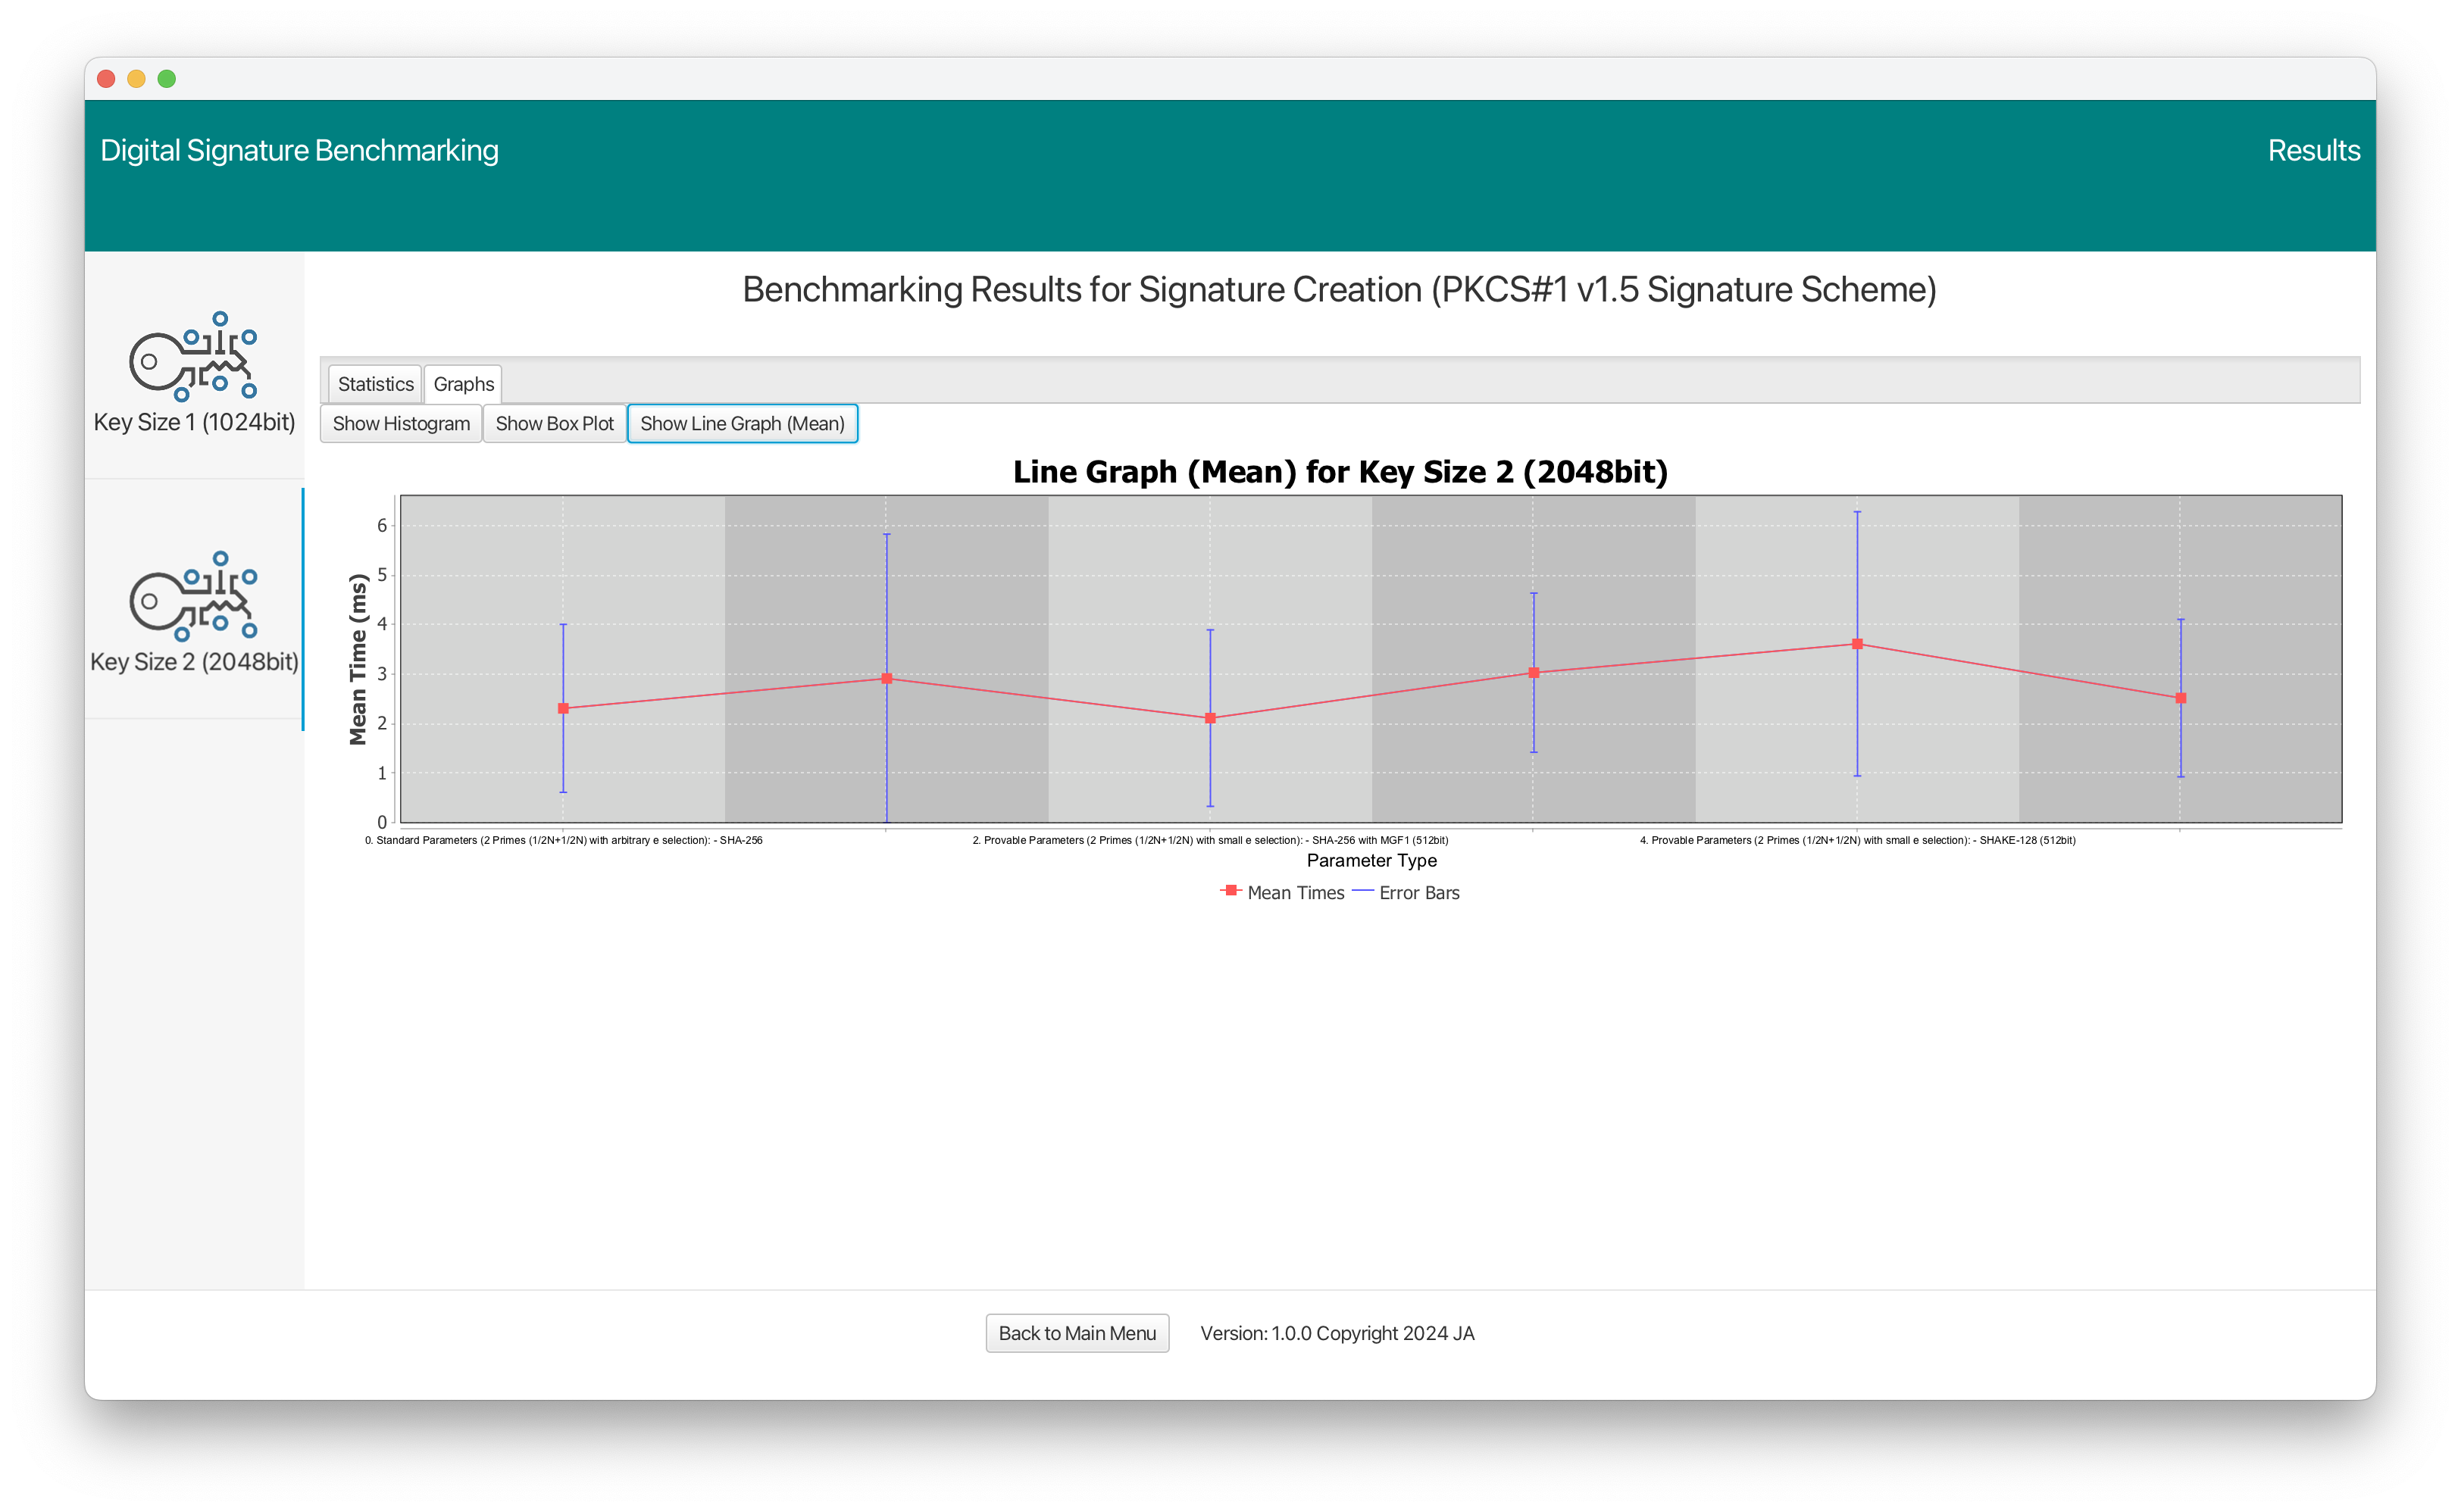
\includegraphics[width=\textwidth]{main_pictures/ui/signing/signing10-2.png}} % Adding border here
       \caption{Comparison Benchmarking: Signature Generation: Overlaid Line graph for mean times}
        \label{fig:image2}
    \end{minipage}
\end{figure}

Signature generation results can also be visualised graphically, accessible under the "Graphs" tab in the central pane. These graphs, correlating with key configurations from the results table, offer an alternate method for interpreting data.


\subsection{Signature Verification}

\begin{figure}[H]
    \centering
    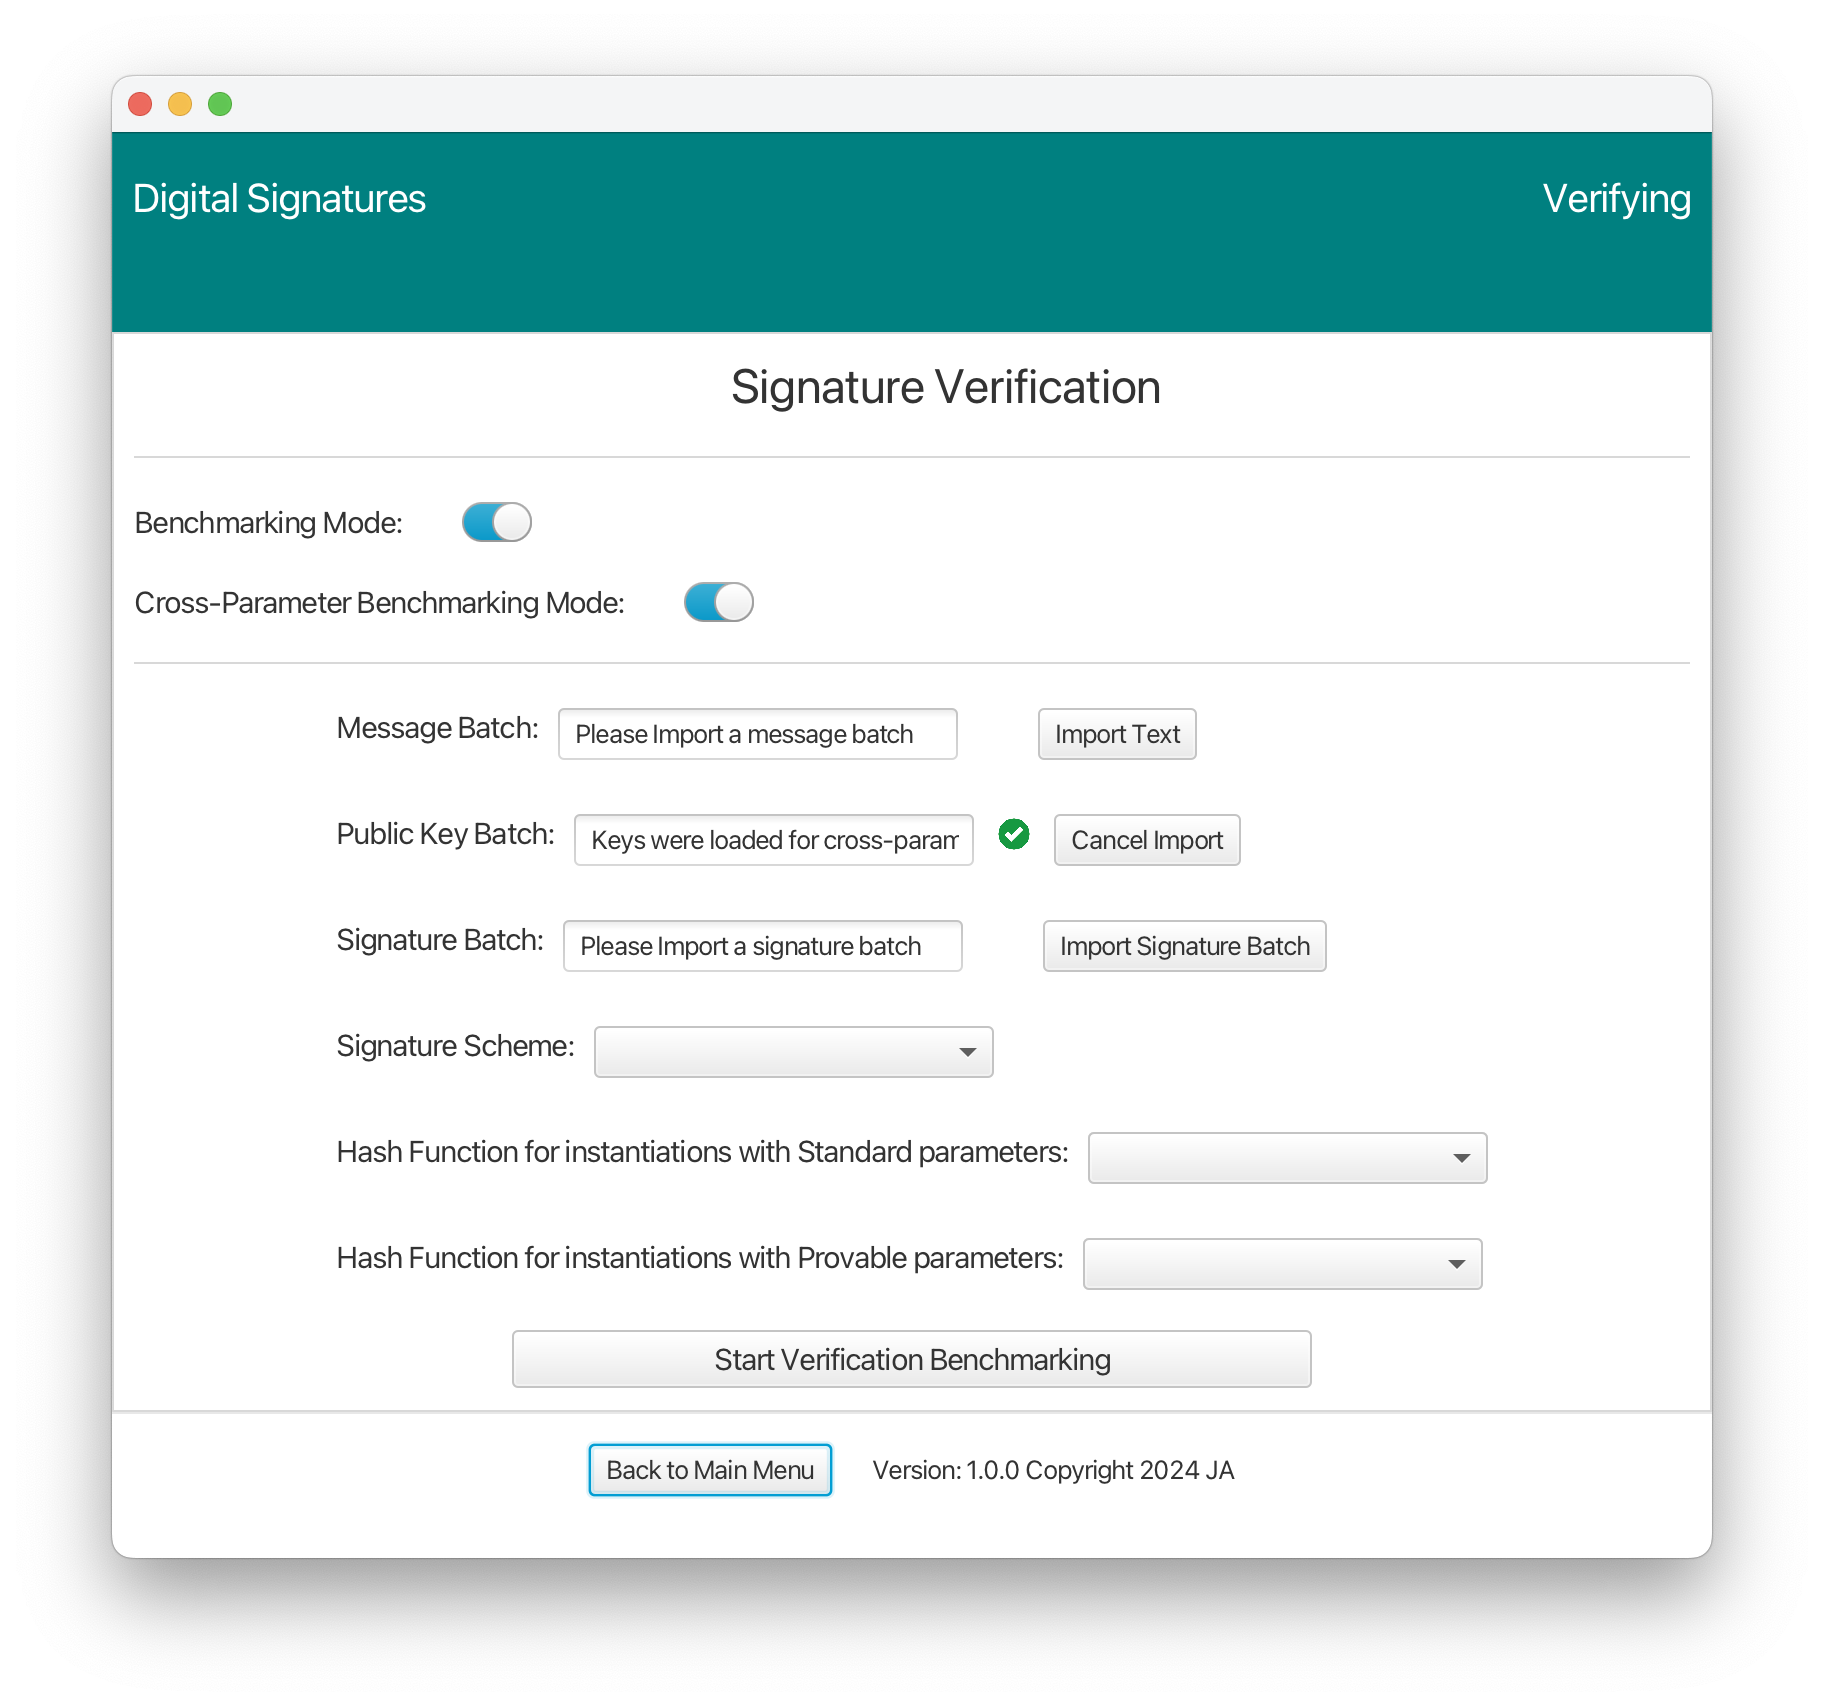
\includegraphics[scale= 0.4]{main_pictures/ui/verifying/verifying0.png}
   \caption{Comparison Benchmarking: Signature Verification (Comparison Benchmarking)}
\end{figure}

Similar to the process for signature generation, the signature verification screen for comparison benchmarking is accessible after completing a key generation benchmark in comparison mode. This procedure also includes preloading a batch of keys. However, the key distinction lies in the type of key batch loaded. In the case of signature verification, it's a public key batch that gets preloaded, as opposed to a private key batch used for signature generation.


\begin{figure}[H]
    \centering % Center the images
    
    % First image in a minipage
    \begin{minipage}{0.4\textwidth}
        \centering
        \fbox{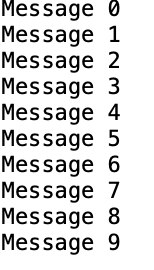
\includegraphics[width=0.4\textwidth]{main_pictures/ui/signing/signing2.png}} % Adding border here
       \caption{Comparison Benchmarking: Signature Verification (Test message batch (testMessages.txt))}
        \label{fig:image1}
    \end{minipage}
    \hfill % Add some space between the images
    % Second image in a minipage
    \begin{minipage}{0.58\textwidth}
        \centering
        \fbox{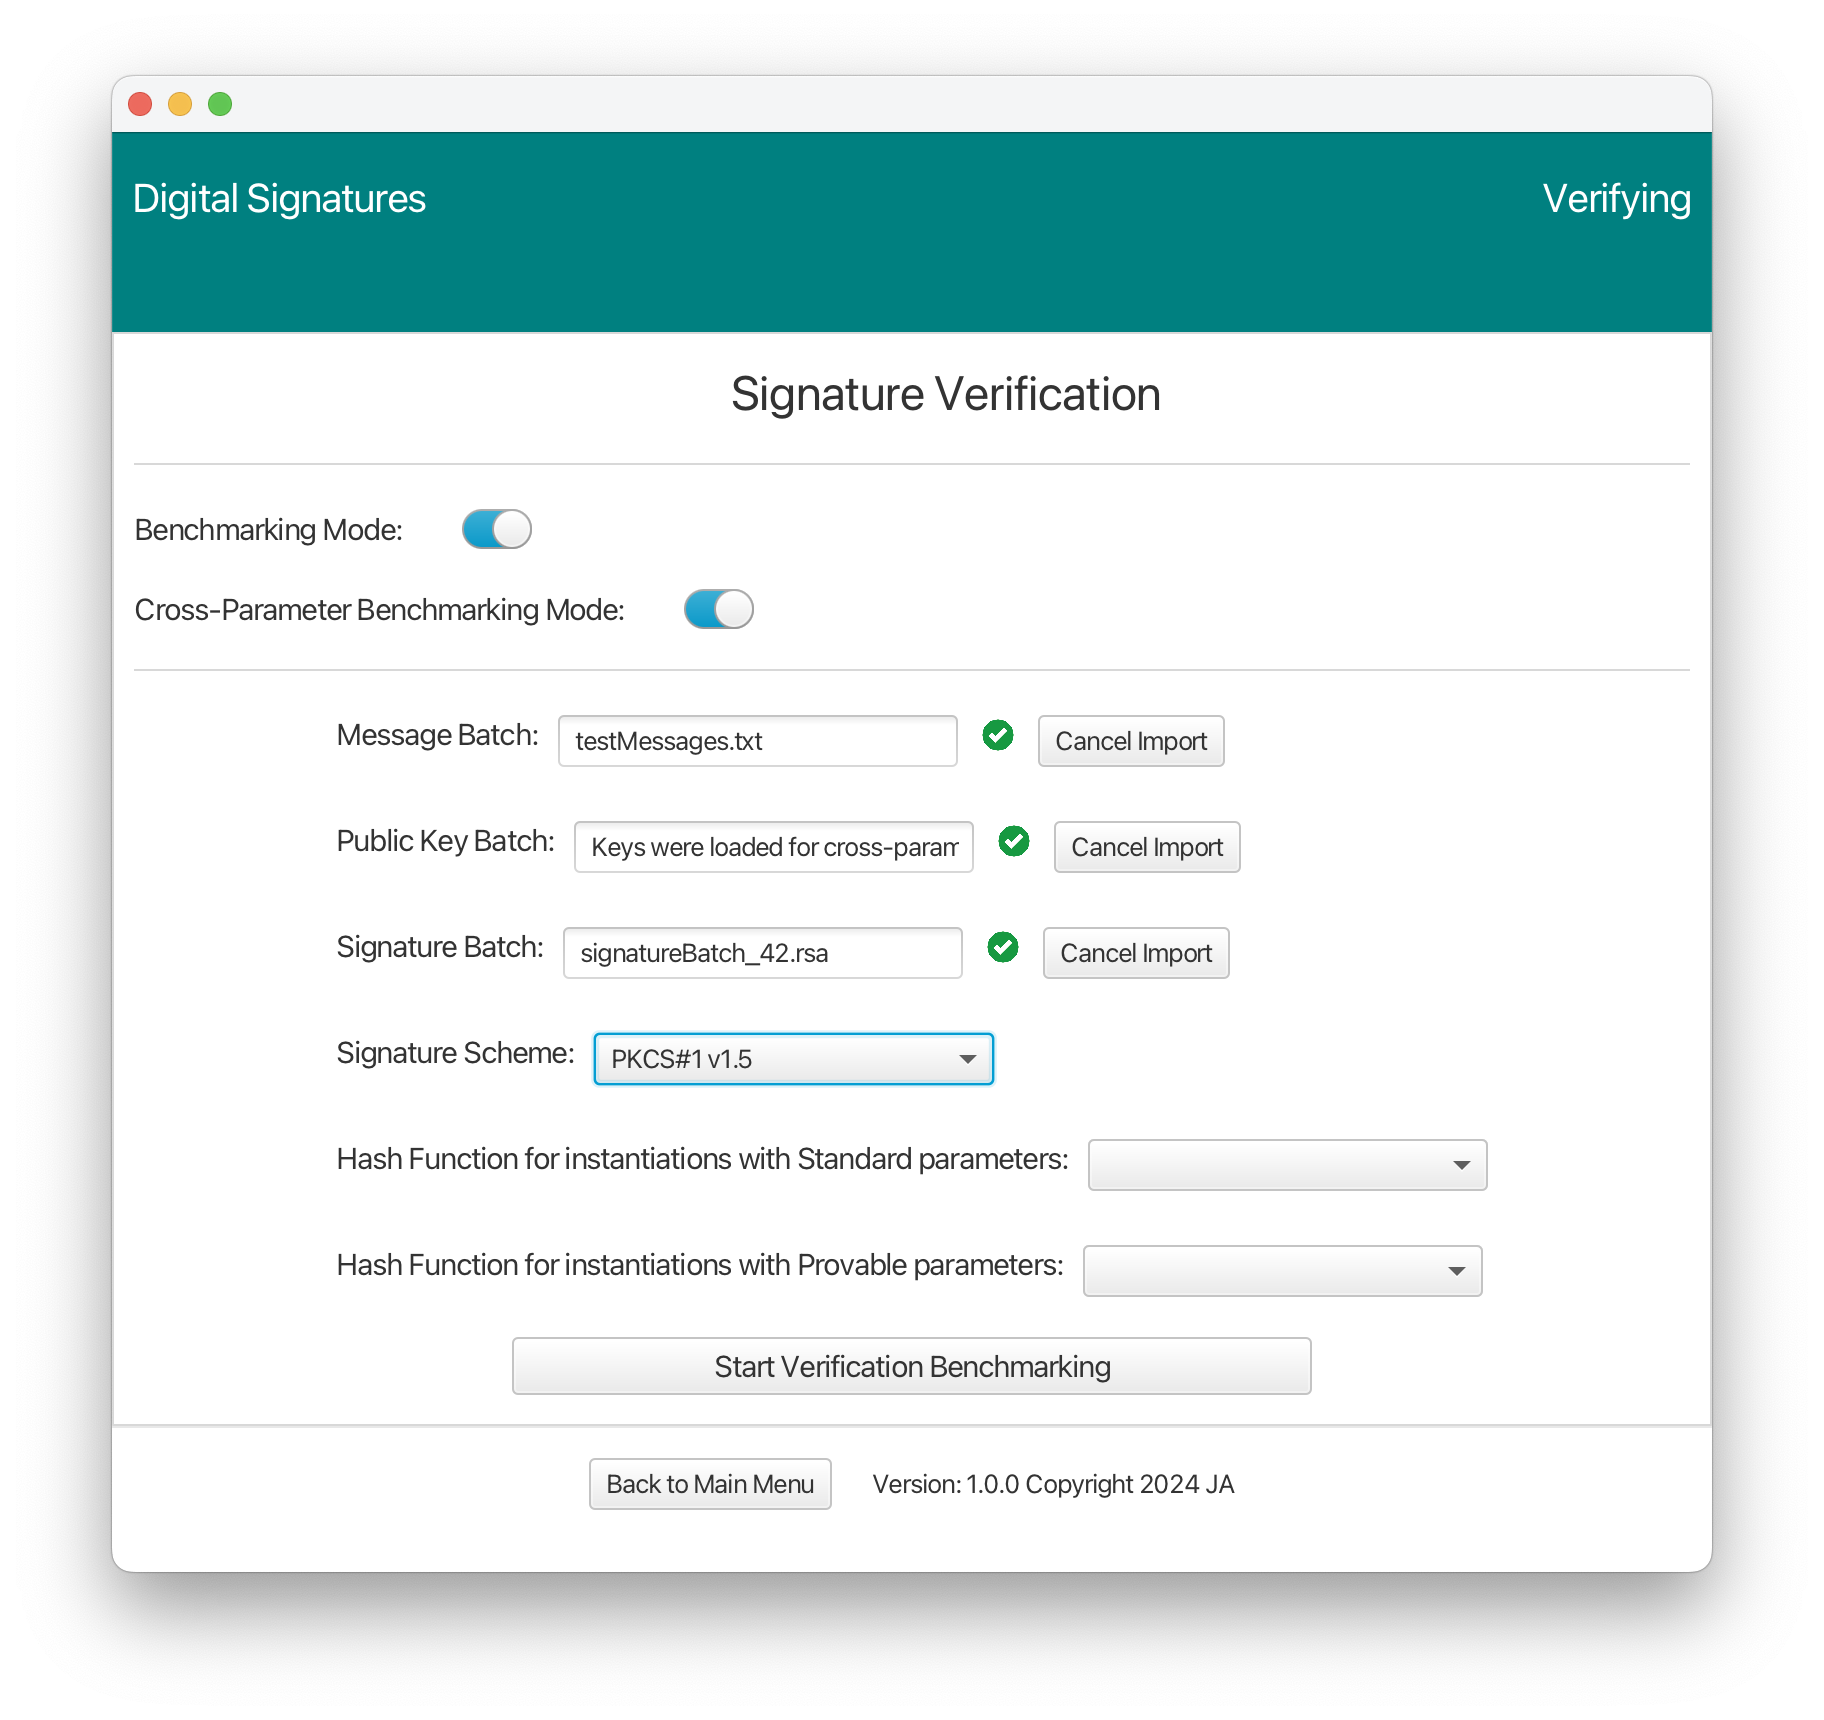
\includegraphics[width=\textwidth]{main_pictures/ui/verifying/verifying2.png}} % Adding border here
       \caption{Comparison Benchmarking: Signature Verification (Imported message batch)}
        \label{fig:image2}
    \end{minipage}
\end{figure}

Aside from the preloaded public key batch used for comparison benchmarking, the signature verification screen includes fields for importing both message and signature batches. For correctness, it's necessary that the submitted message batch aligns with the submitted signature batch. Moreover, these batches must be compatible with the public key batch, which, in turn, is associated with the private key batch employed during the prior signature generation phase.


\begin{figure}[H]
    \centering % Center the images
    
    % First image in a minipage
    \begin{minipage}{0.49\textwidth}
        \centering
        \fbox{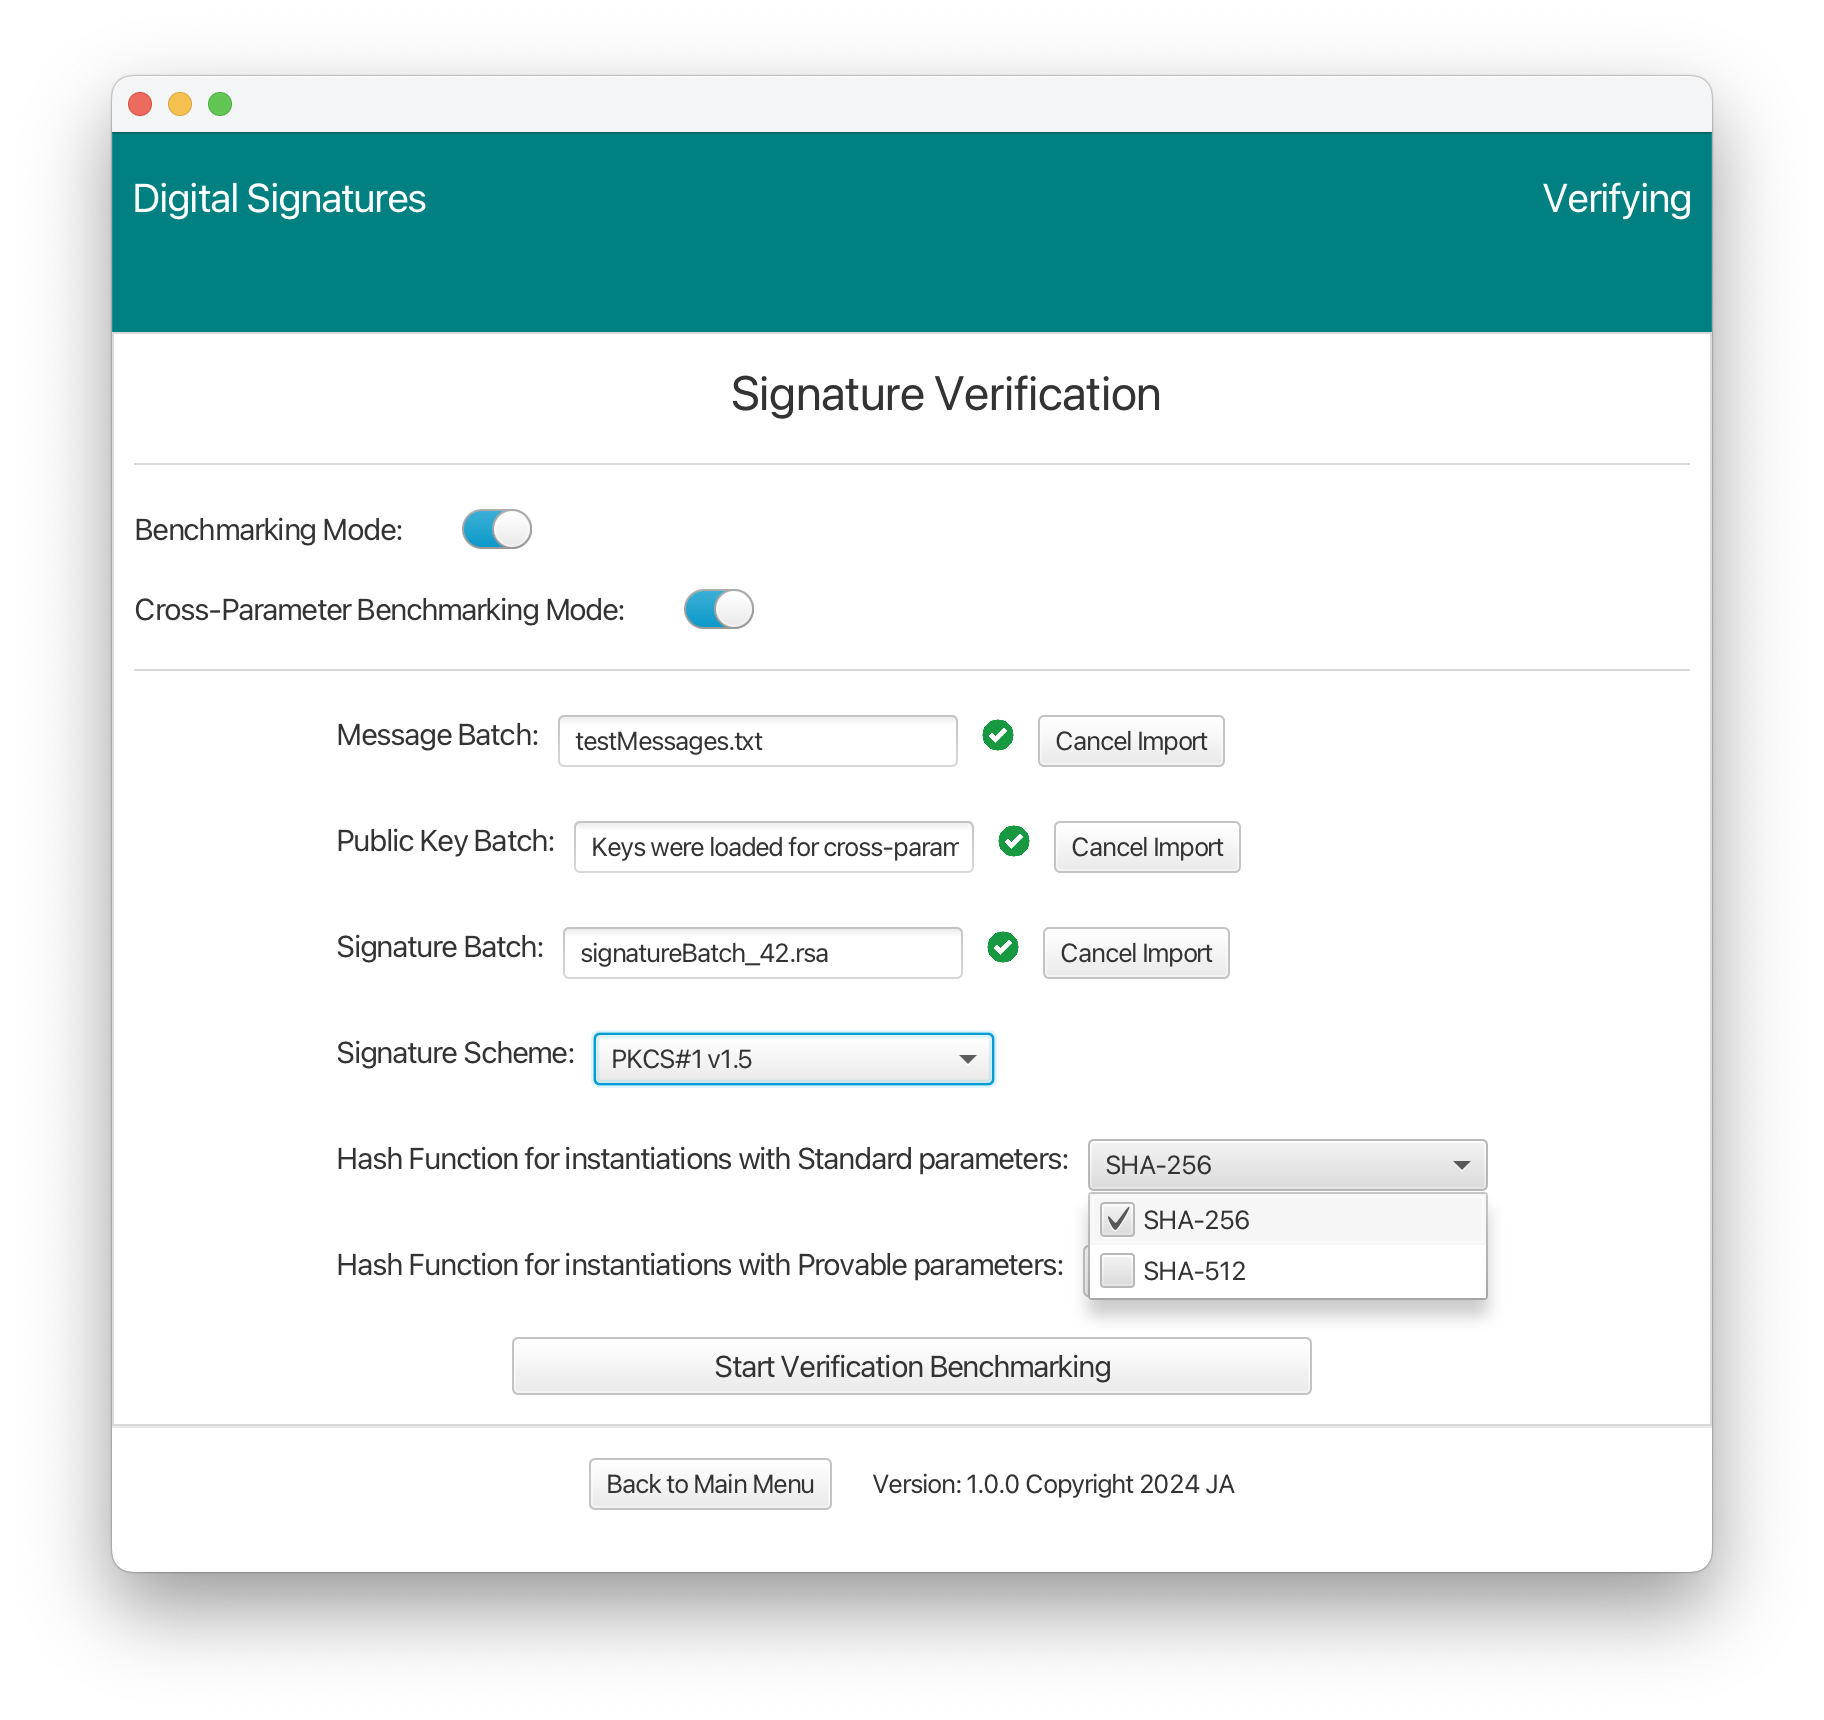
\includegraphics[width=\textwidth]{main_pictures/ui/verifying/verifying3.png}} % Adding border here
       \caption{Comparison Benchmarking: Signature Verification (Standard Parameter Hash Functions)}
        \label{fig:image1}
    \end{minipage}
    \hfill % Add some space between the images
    % Second image in a minipage
    \begin{minipage}{0.49\textwidth}
        \centering
        \fbox{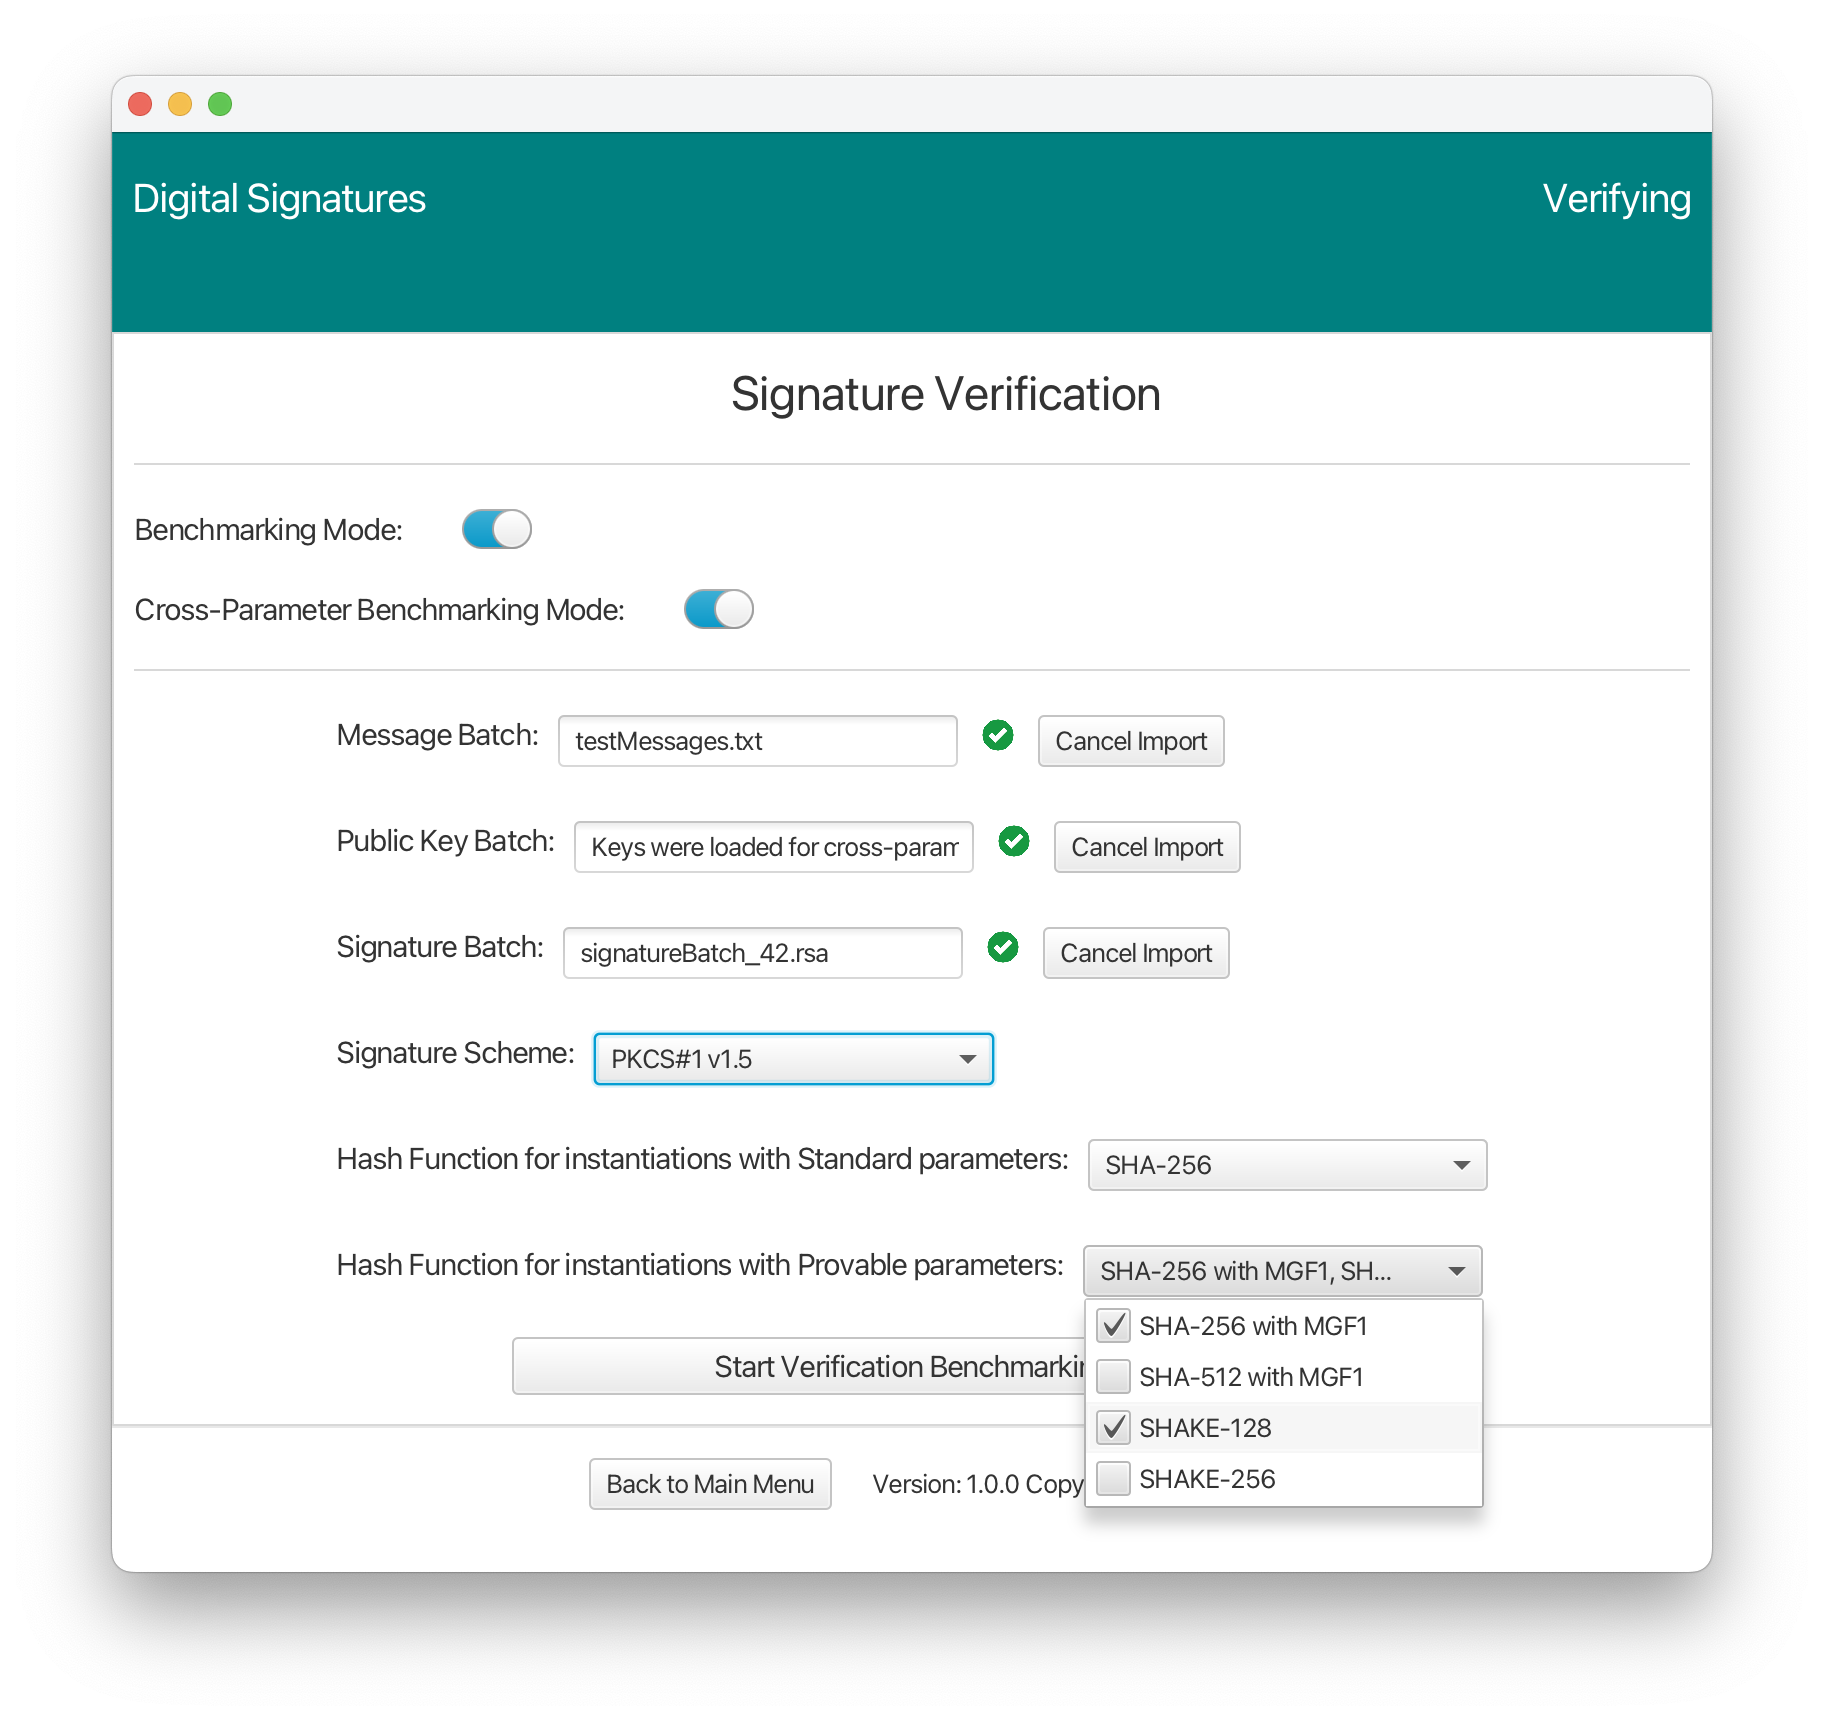
\includegraphics[width=\textwidth]{main_pictures/ui/verifying/verifying4.png}} % Adding border here
       \caption{Comparison Benchmarking: Signature Verification (Provably Secure Parameter Hash Functions)}
        \label{fig:image2}
    \end{minipage}
\end{figure}


In signature verification (comparison) benchmarking, hash function selection must align with those used in signature generation to ensure correctness. The process starts with the user choosing matching hash functions for each parameter type. This is vital because the hash functions used must correspond to the message-signature pairs created in the signature generation phase, which used the private key batch related to the currently imported public key batch.

Upon selecting "Start Verification Benchmarking," the application validates the number of signatures against the message batch and chosen hash functions.  Following successful validation,  verification benchmarking is executed . This involves comparing the signature batch with the message batch and public keys, using the selected signature scheme and hash functions. The process generates batches of verification results for each entered key size, and a progress bar provides real-time progress updates.


\textbf{Comparison Benchmarking: Signature Verification Results Screen}

\begin{figure}[H]
    \centering
    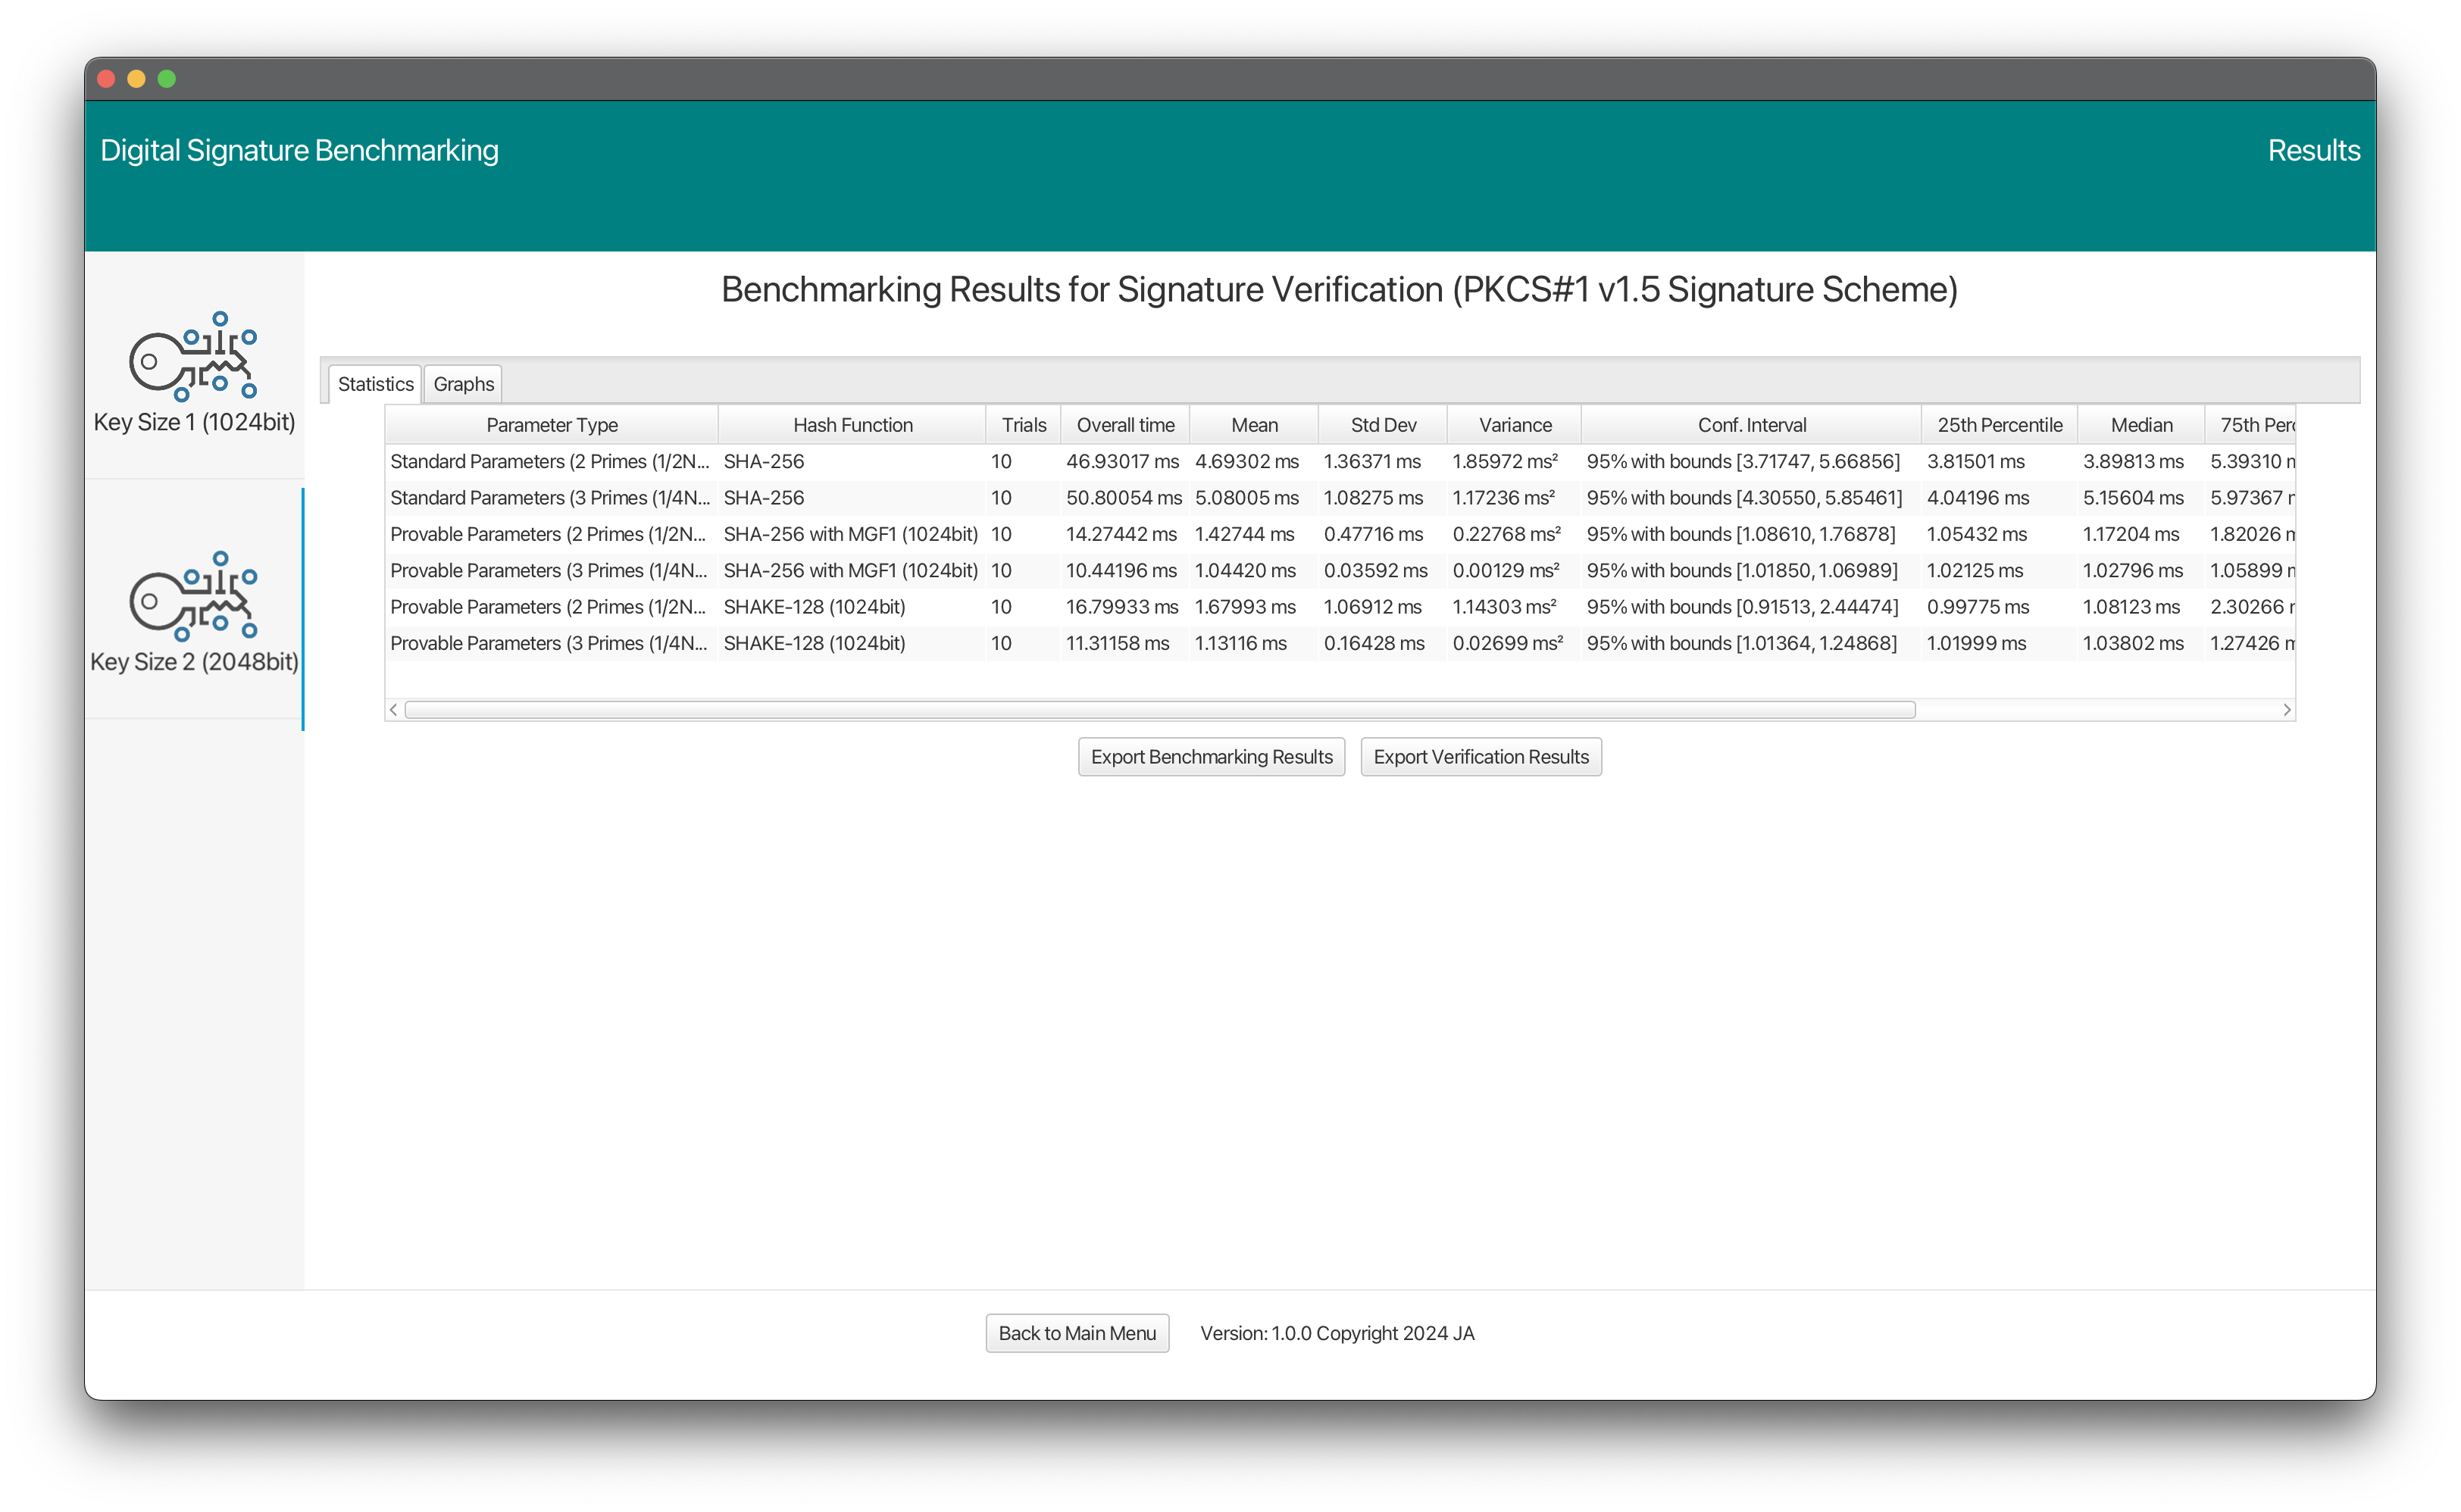
\includegraphics[scale= 0.325]{main_pictures/ui/verifying/verifying6.png}
   \caption{Comparison Benchmarking: Signature Verification (Results Screen)}
\end{figure}

Once the signature verification benchmarking concludes, results from benchmarking are displayed. The layout of this results screen is largely as was shown for signature generation. The distinction is the enabling of the export of verification results for each key size, displayed below each results table.

\textbf{Comparison Benchmarking: Signature Verification Results Screen Graphs}


\begin{figure}[H]
    \centering % Center the images
    
    % First image in a minipage
    \begin{minipage}{0.7\textwidth}
        \centering
        \fbox{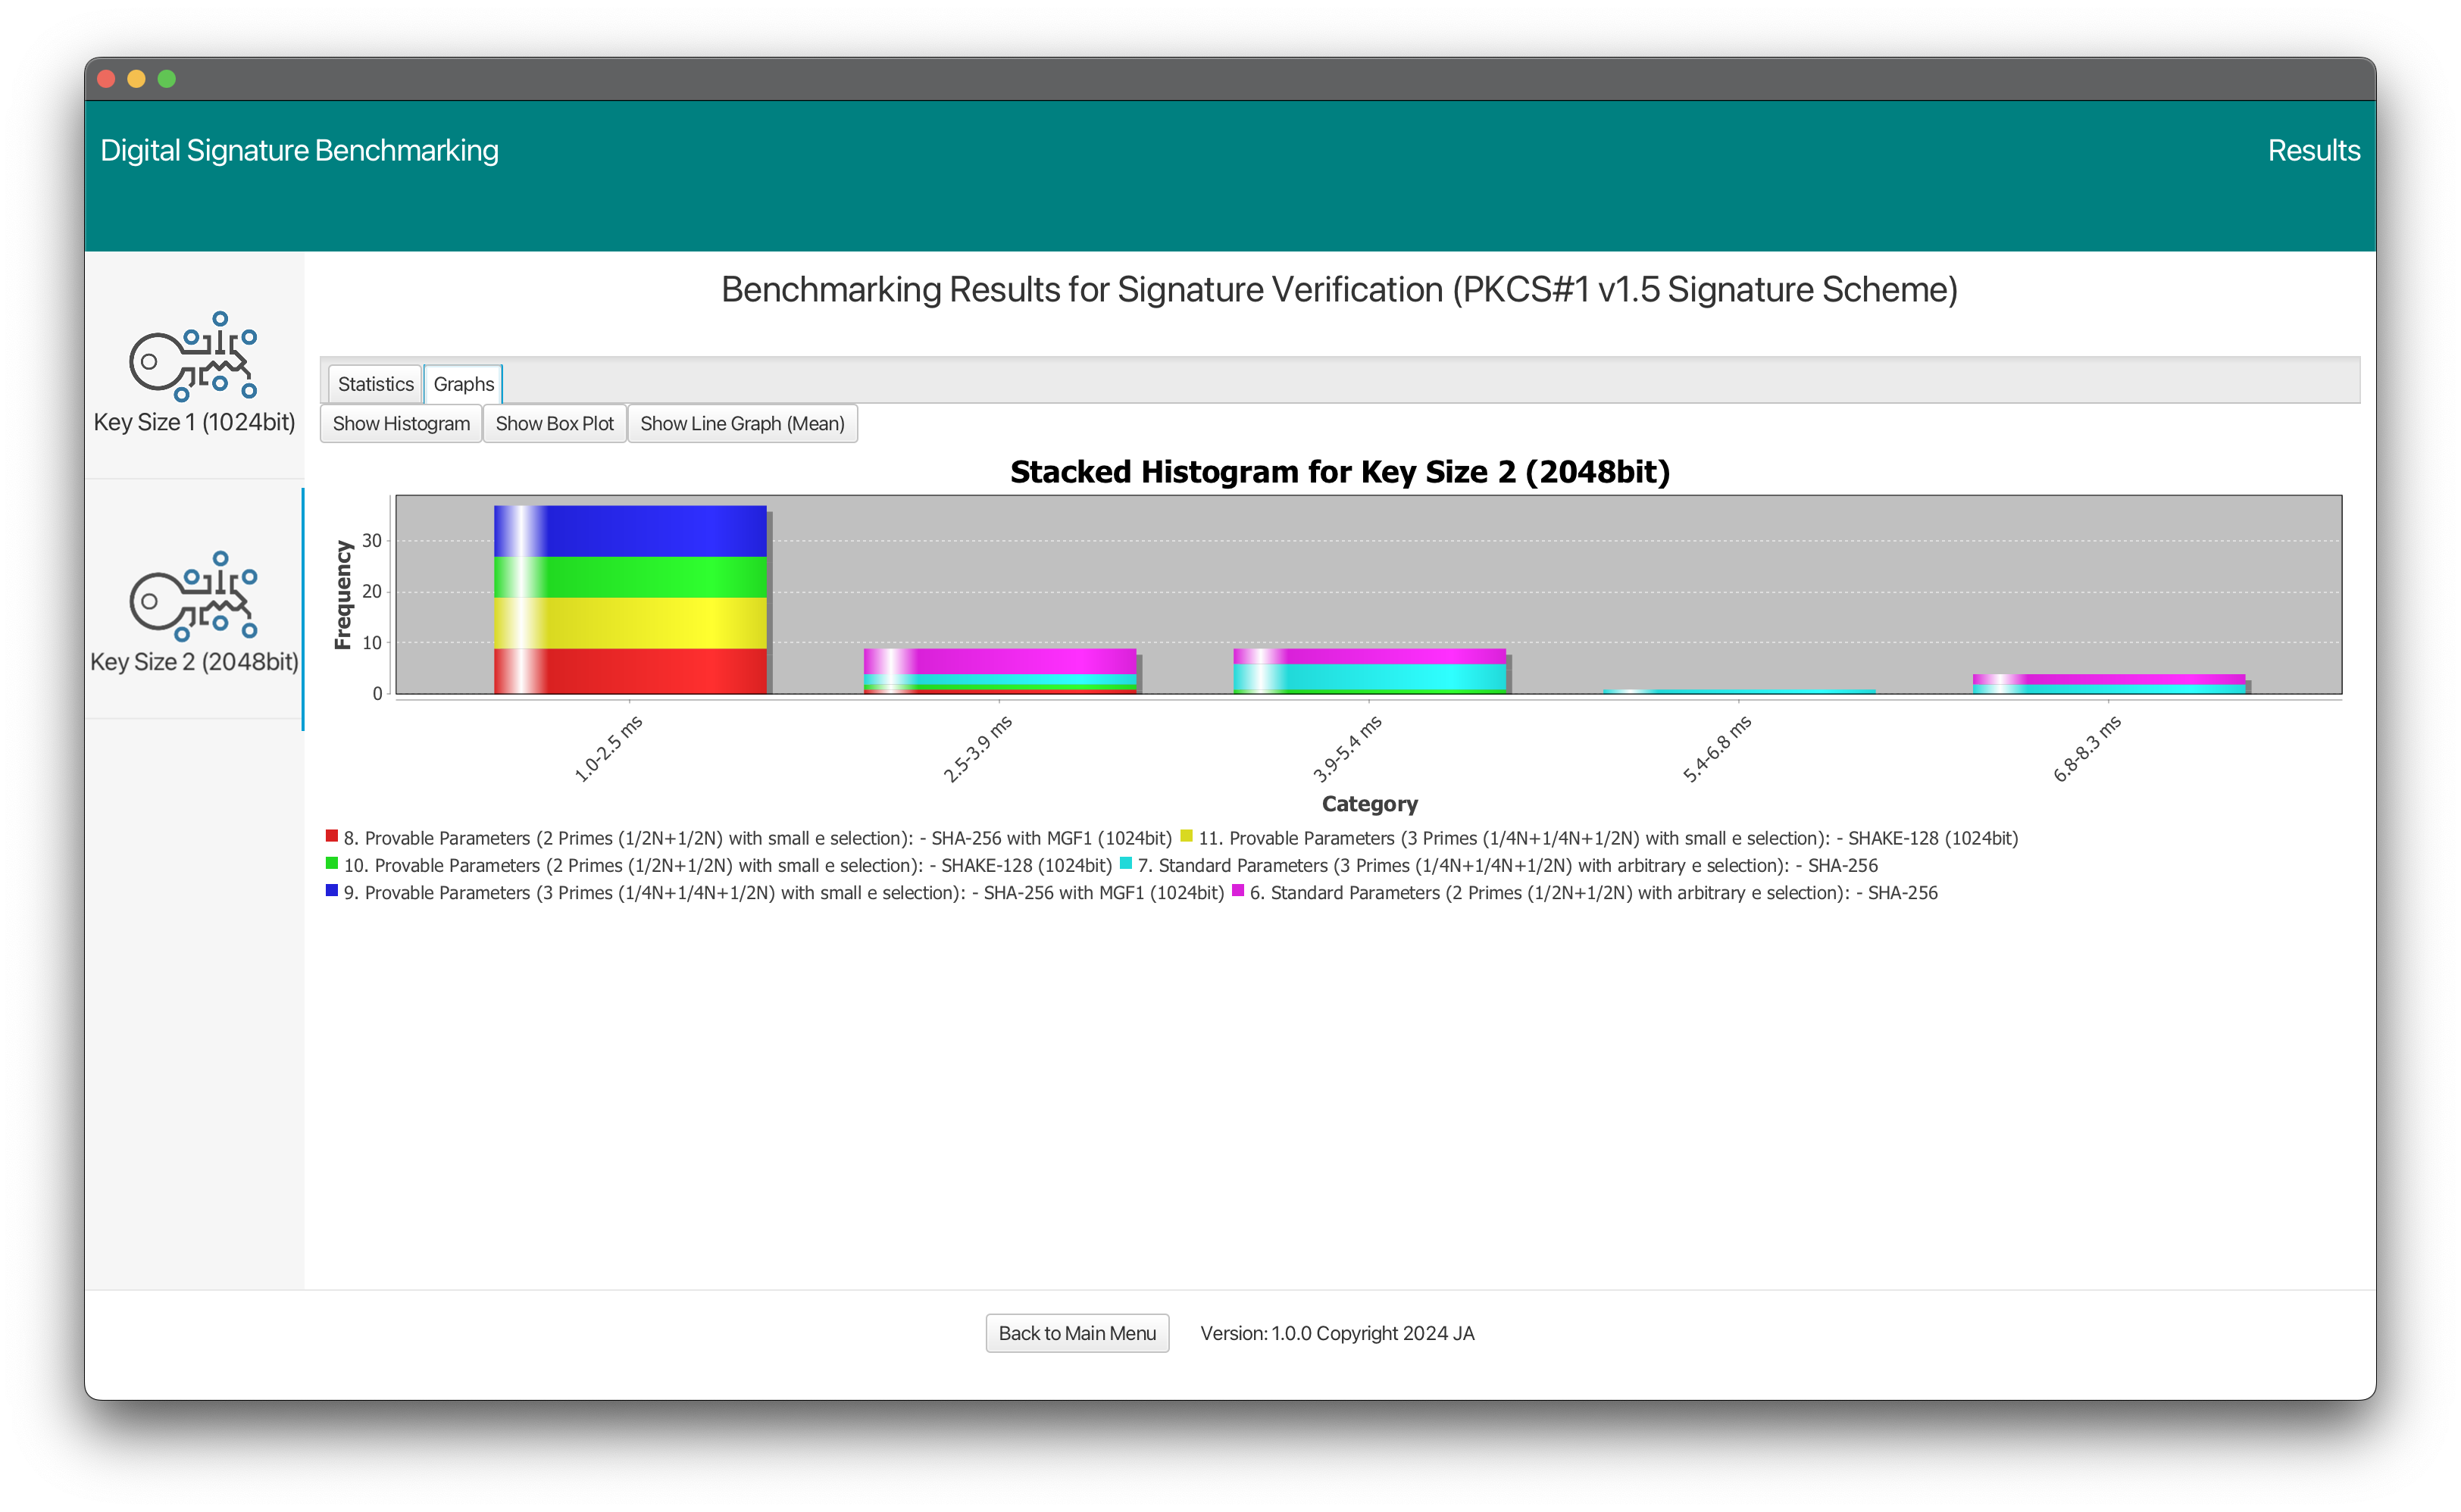
\includegraphics[width=\textwidth]{main_pictures/ui/verifying/verifying7.png}} % Adding border here
       \caption{Comparison Benchmarking: Signature Verification: Overlaid Histogram}
        \label{fig:image1}
    \end{minipage}
    \hfill % Add some space between the images
    % Second image in a minipage
    \begin{minipage}{0.7\textwidth}
        \centering
        \fbox{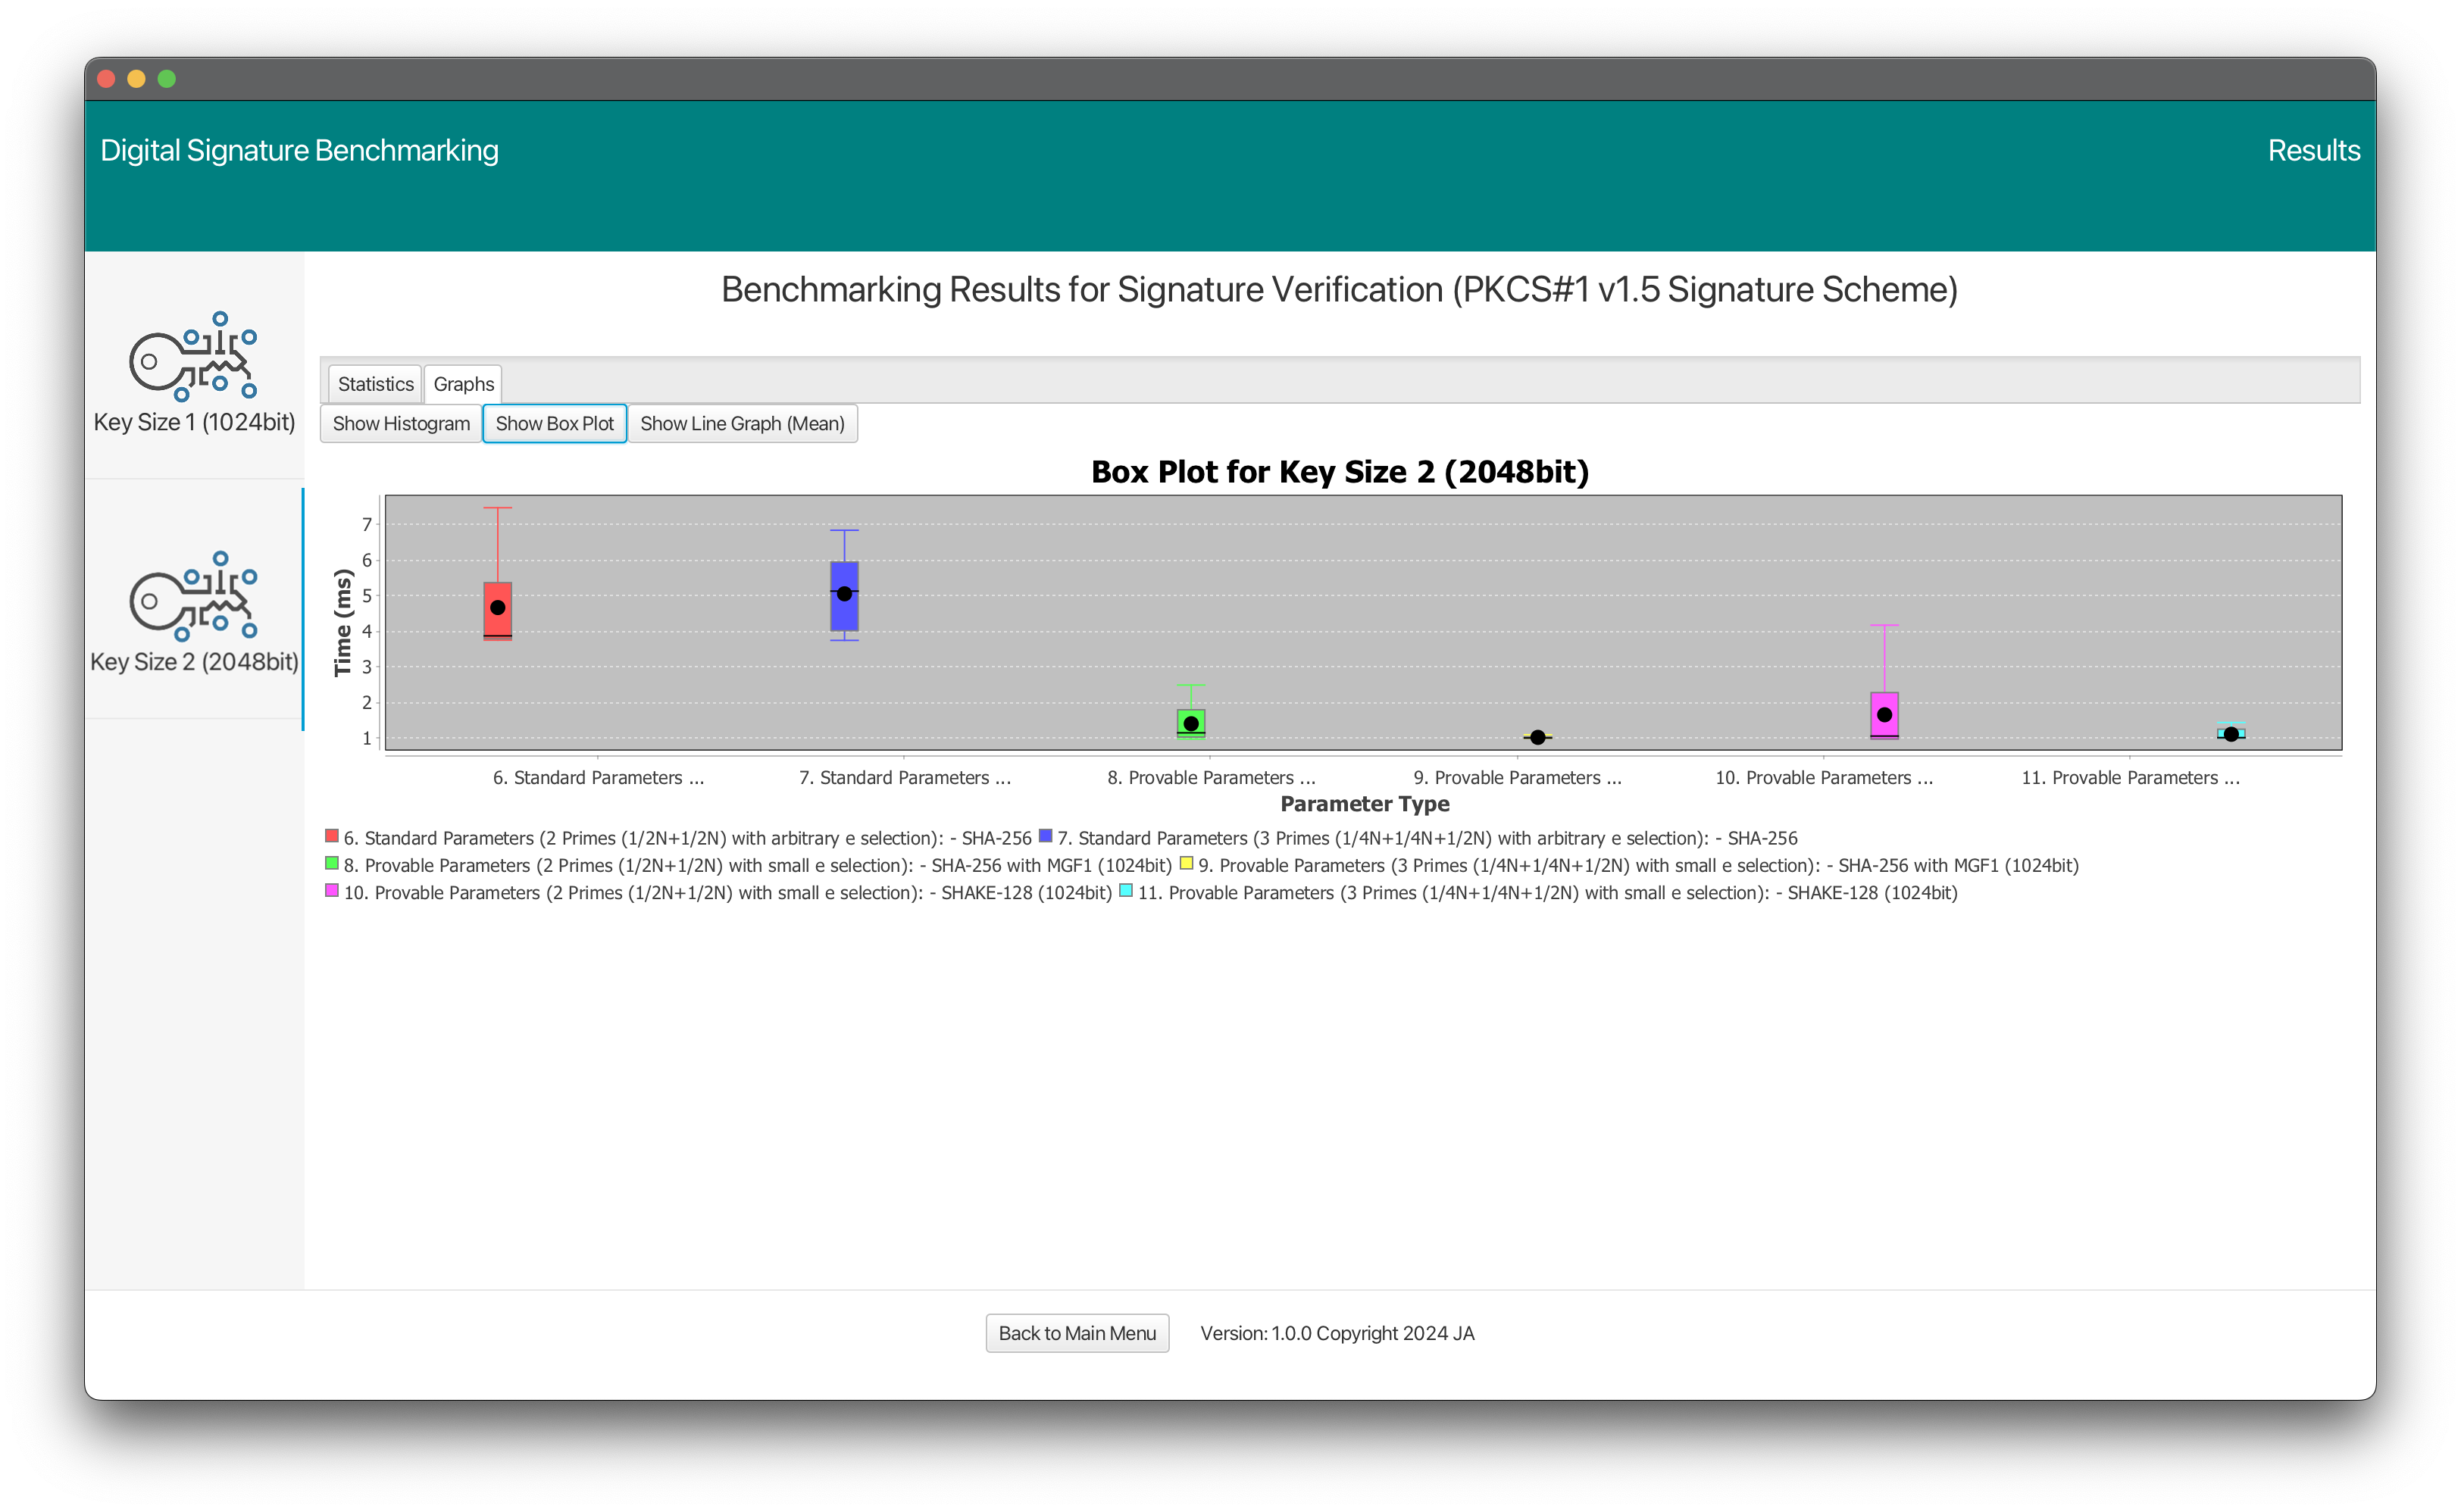
\includegraphics[width=\textwidth]{main_pictures/ui/verifying/verifying8.png}} % Adding border here
       \caption{Comparison Benchmarking: Signature Verification: Overlaid Box plot graph}
        \label{fig:image2} 
    \end{minipage}
     \begin{minipage}{0.7\textwidth}
        \centering
        \fbox{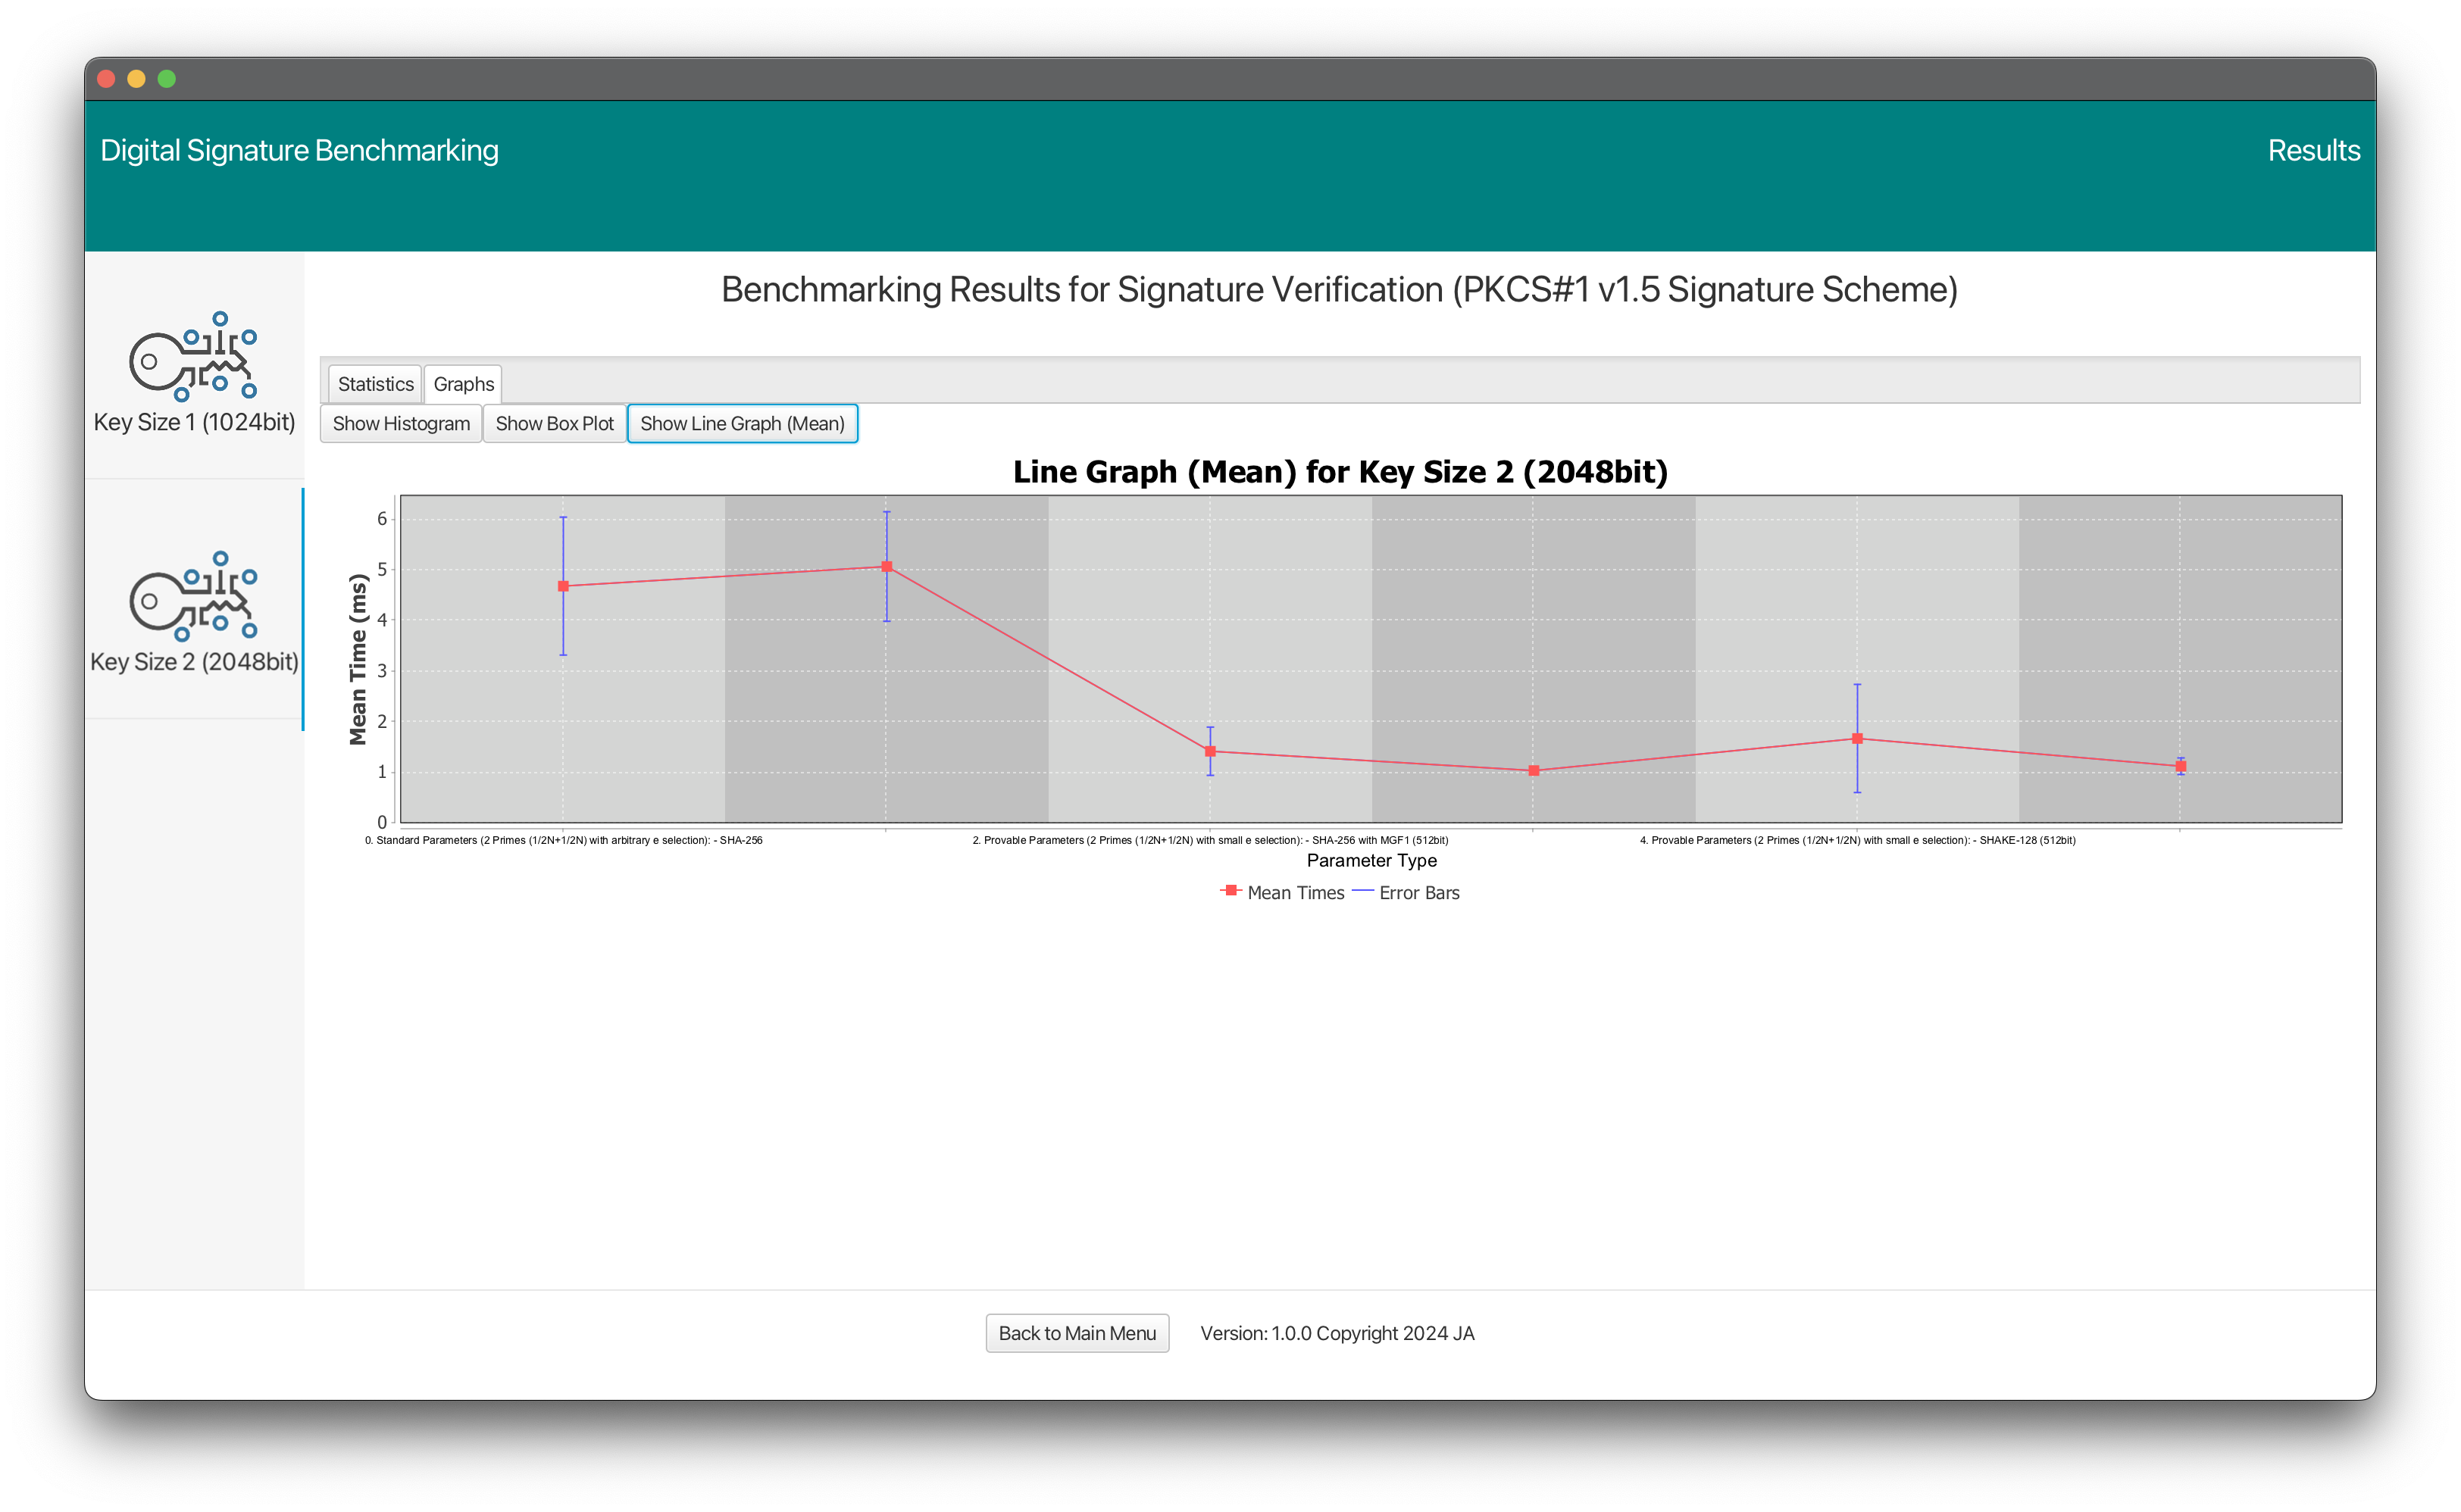
\includegraphics[width=\textwidth]{main_pictures/ui/verifying/verifying9.png}} % Adding border here
       \caption{Comparison Benchmarking: Signature Verification: Overlaid Line graph for mean times}
        \label{fig:image2}
    \end{minipage}
\end{figure}


\chapter{Custom Comparison Benchmarking (Standard vs. Provably Secure)}
\subsection{Key Generation}
\begin{figure}[H]
    \centering % Center the images
    
    % First image in a minipage
    \begin{minipage}{0.495\textwidth}
        \centering
        \fbox{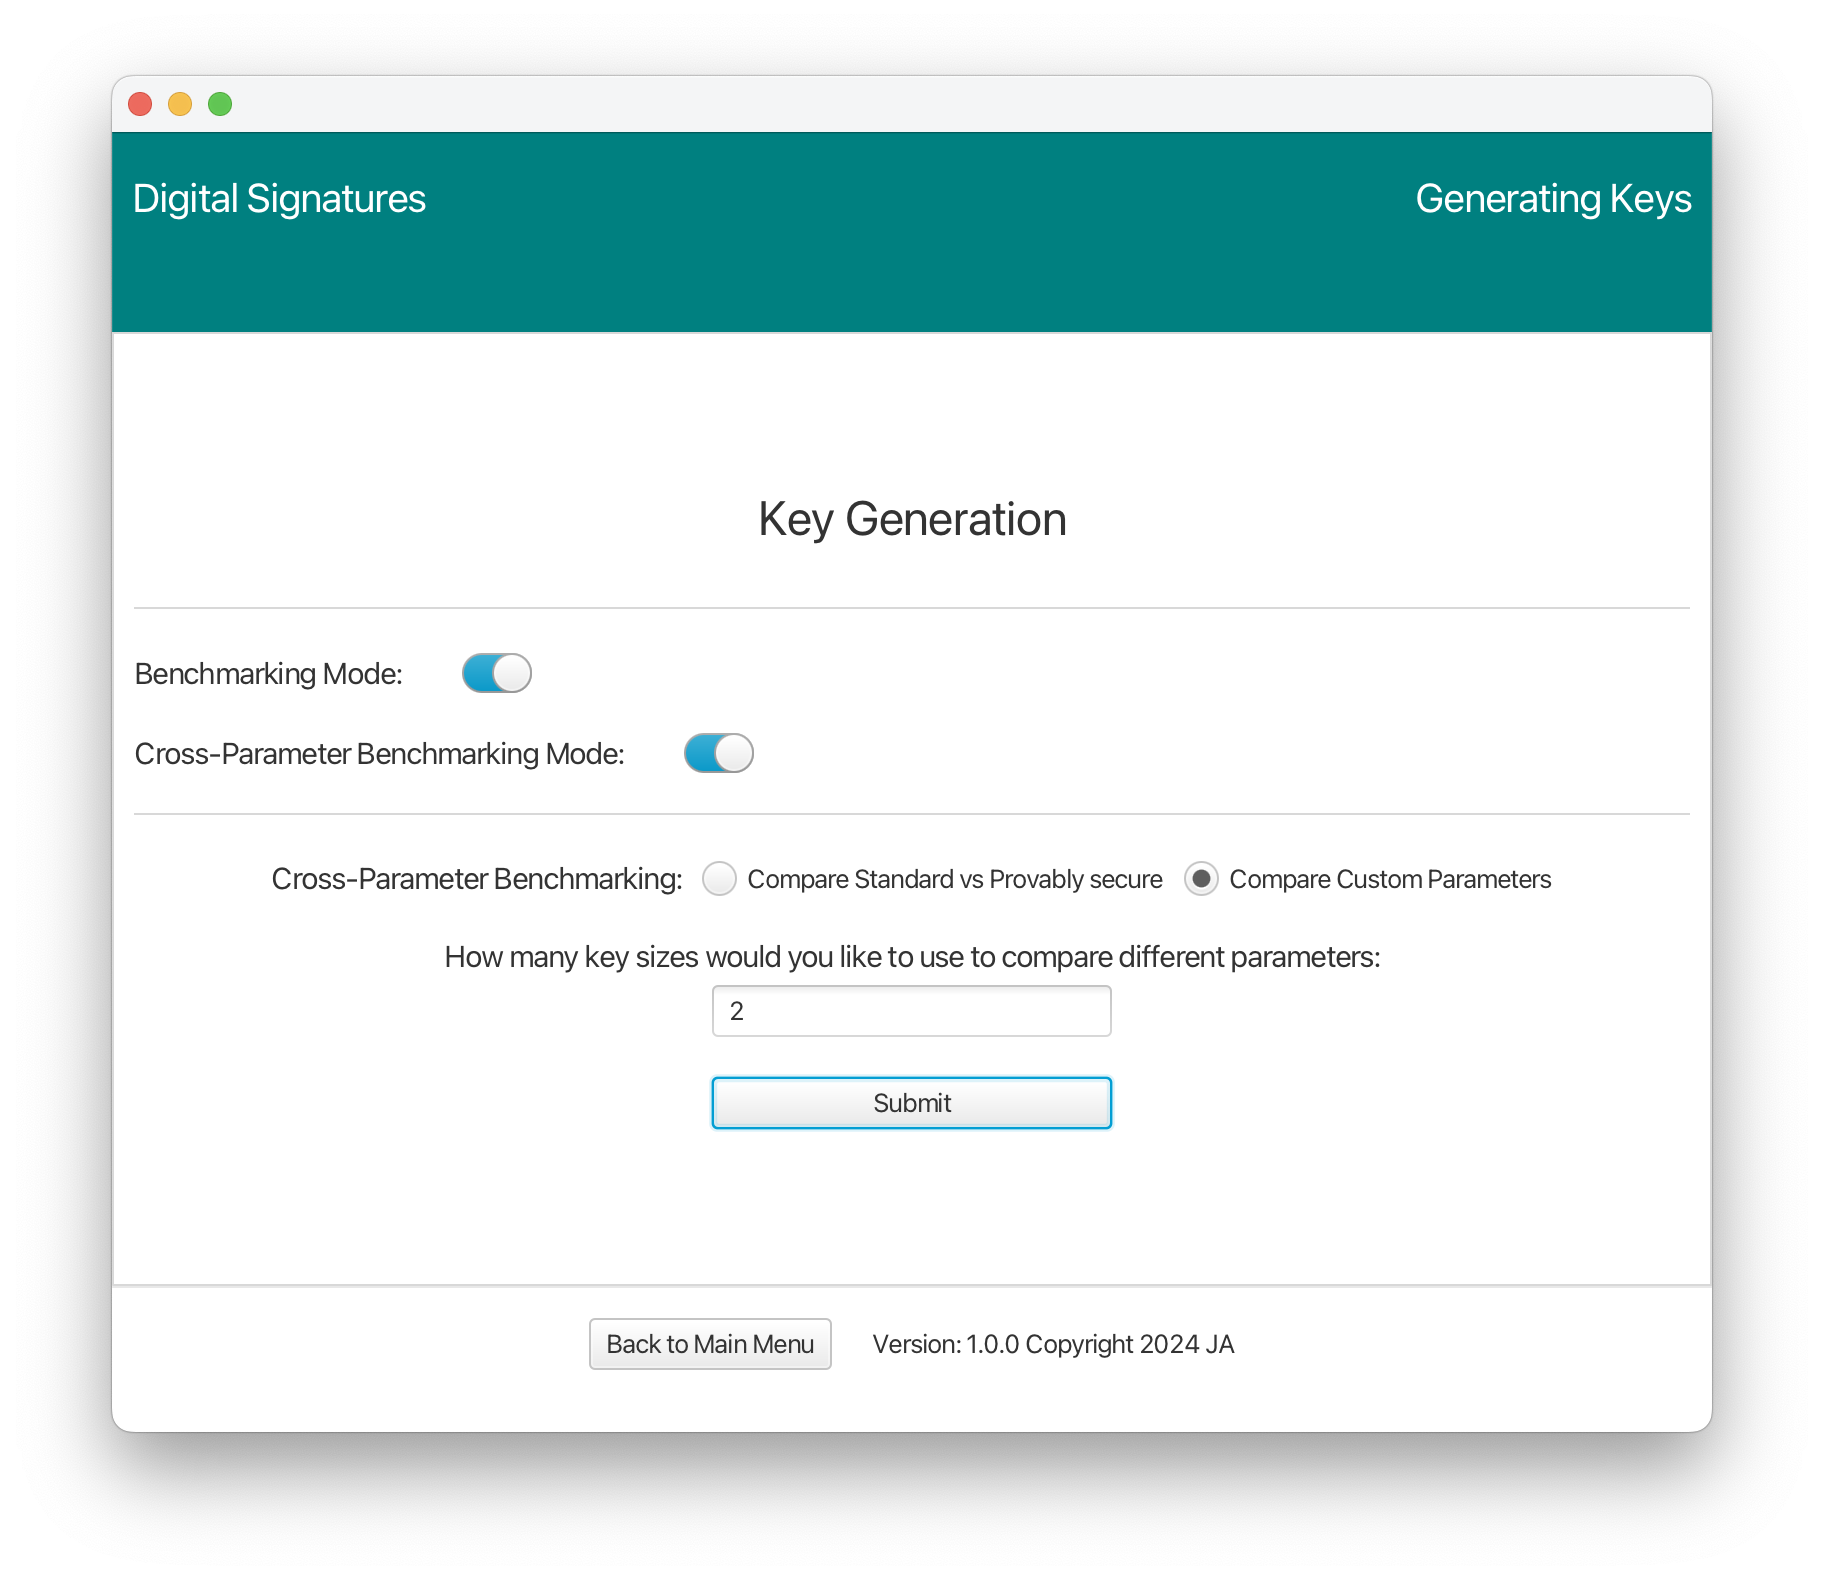
\includegraphics[width=\textwidth]{main_pictures/ui/custom1.png}} % Adding border here
       \caption{Custom Comparison Benchmarking: Key Generation (number of key sizes)}
        \label{fig:image1}
    \end{minipage}
    \hfill % Add some space between the images
    % Second image in a minipage
    \begin{minipage}{0.495\textwidth}
        \centering
        \fbox{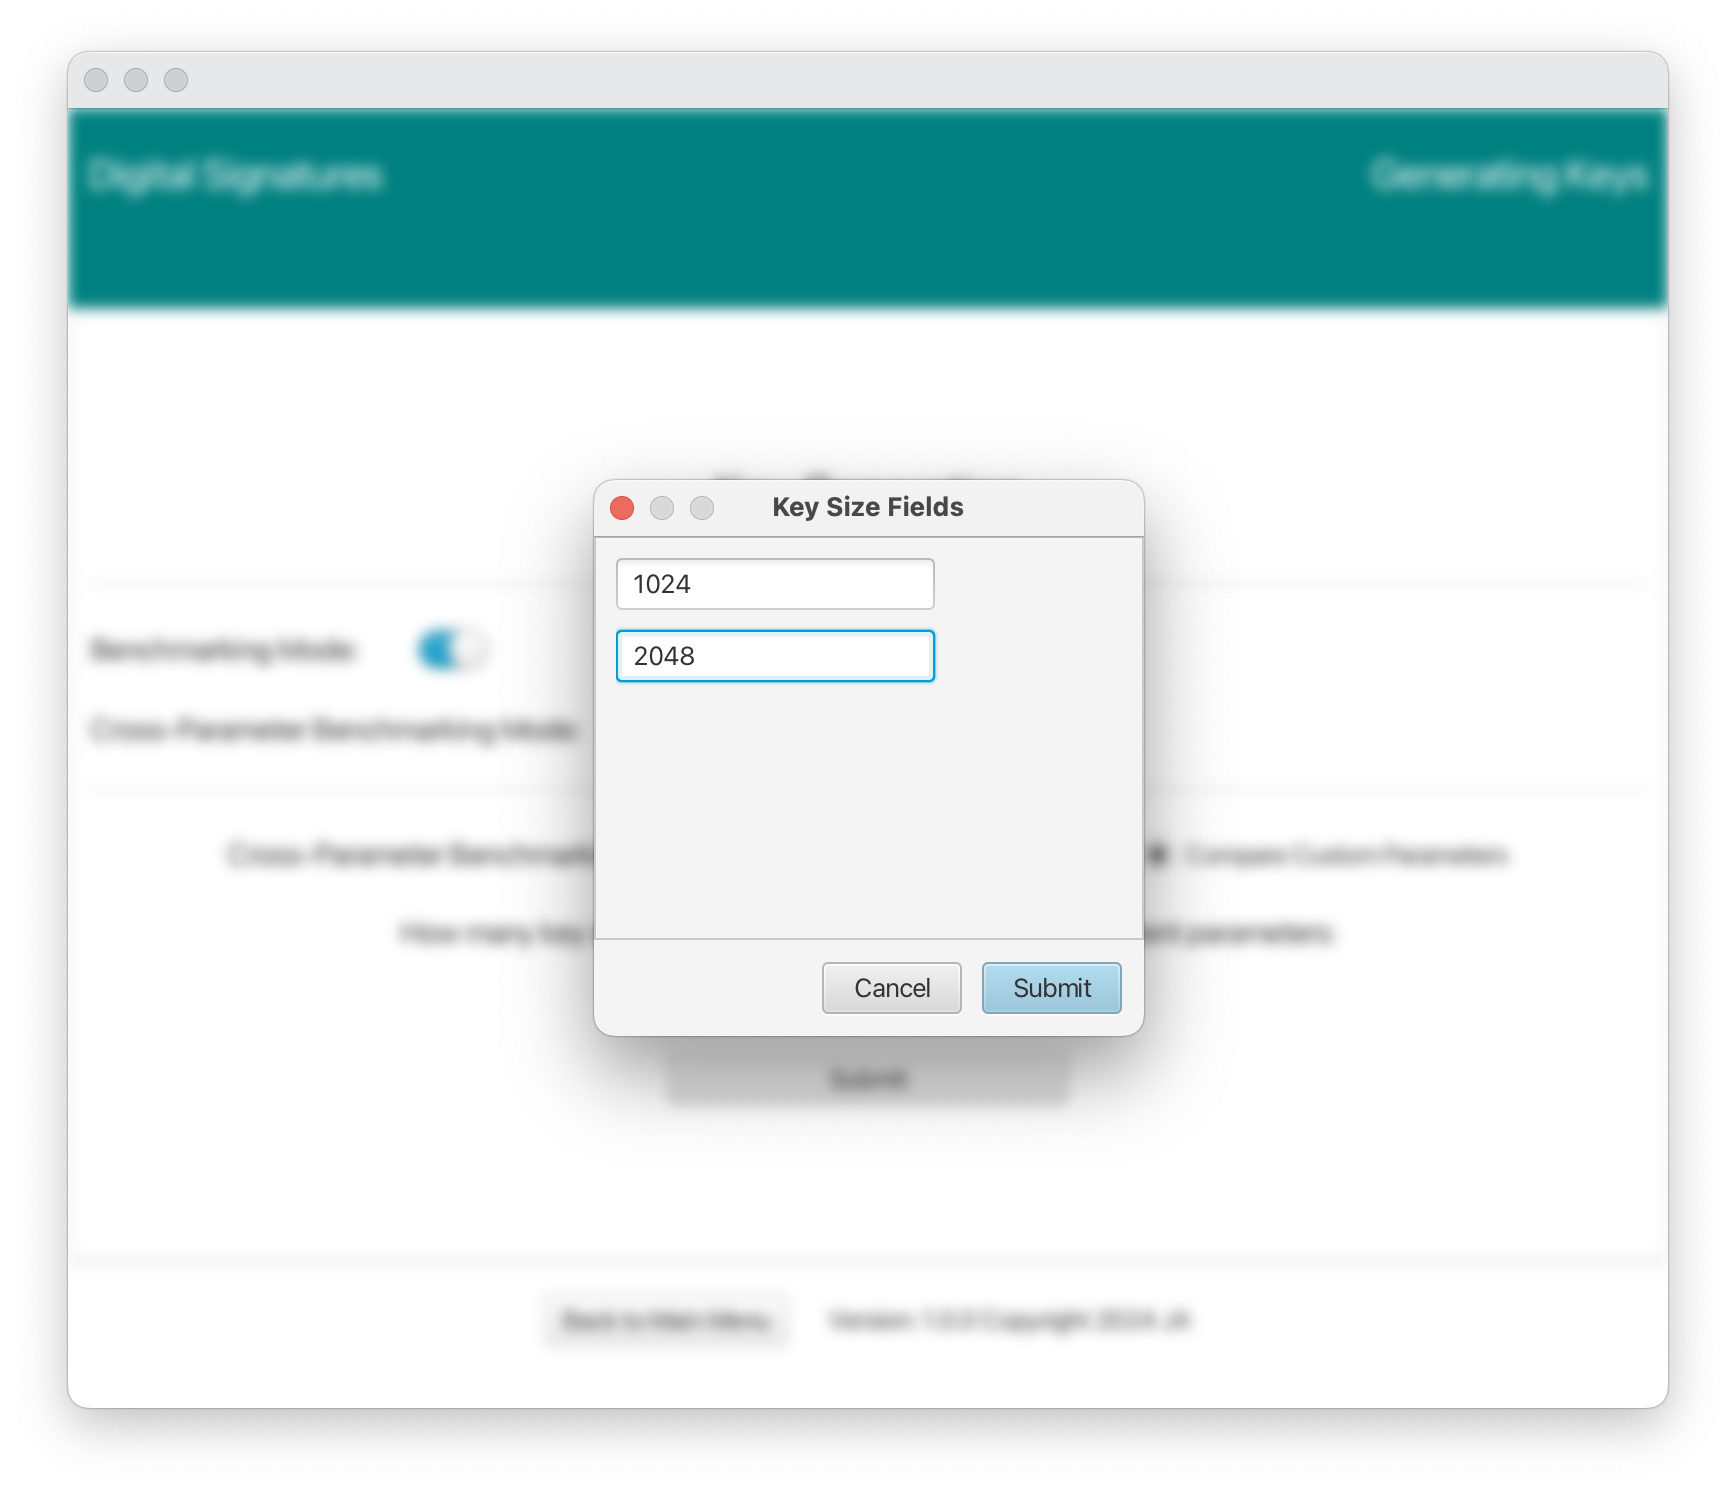
\includegraphics[width=\textwidth]{main_pictures/ui/custom2.png}} % Adding border here
       \caption{Custom Comparison Benchmarking: Key Generation (key sizes)}
        \label{fig:image2}
    \end{minipage}
\end{figure}
The key generation interface for Comparison Benchmarking is activated through a toggle switch. The interface then offers a radio button to select the custom Comparison Benchmarking mode. Initially the flow is same as default comparison benchmarking mode. Users specify the number of key sizes they wish to test, and corresponding input fields are displayed for each size (e.g., Key Size 1: 1024, Key Size 2: 2048).


\begin{figure}[H]
    \centering
    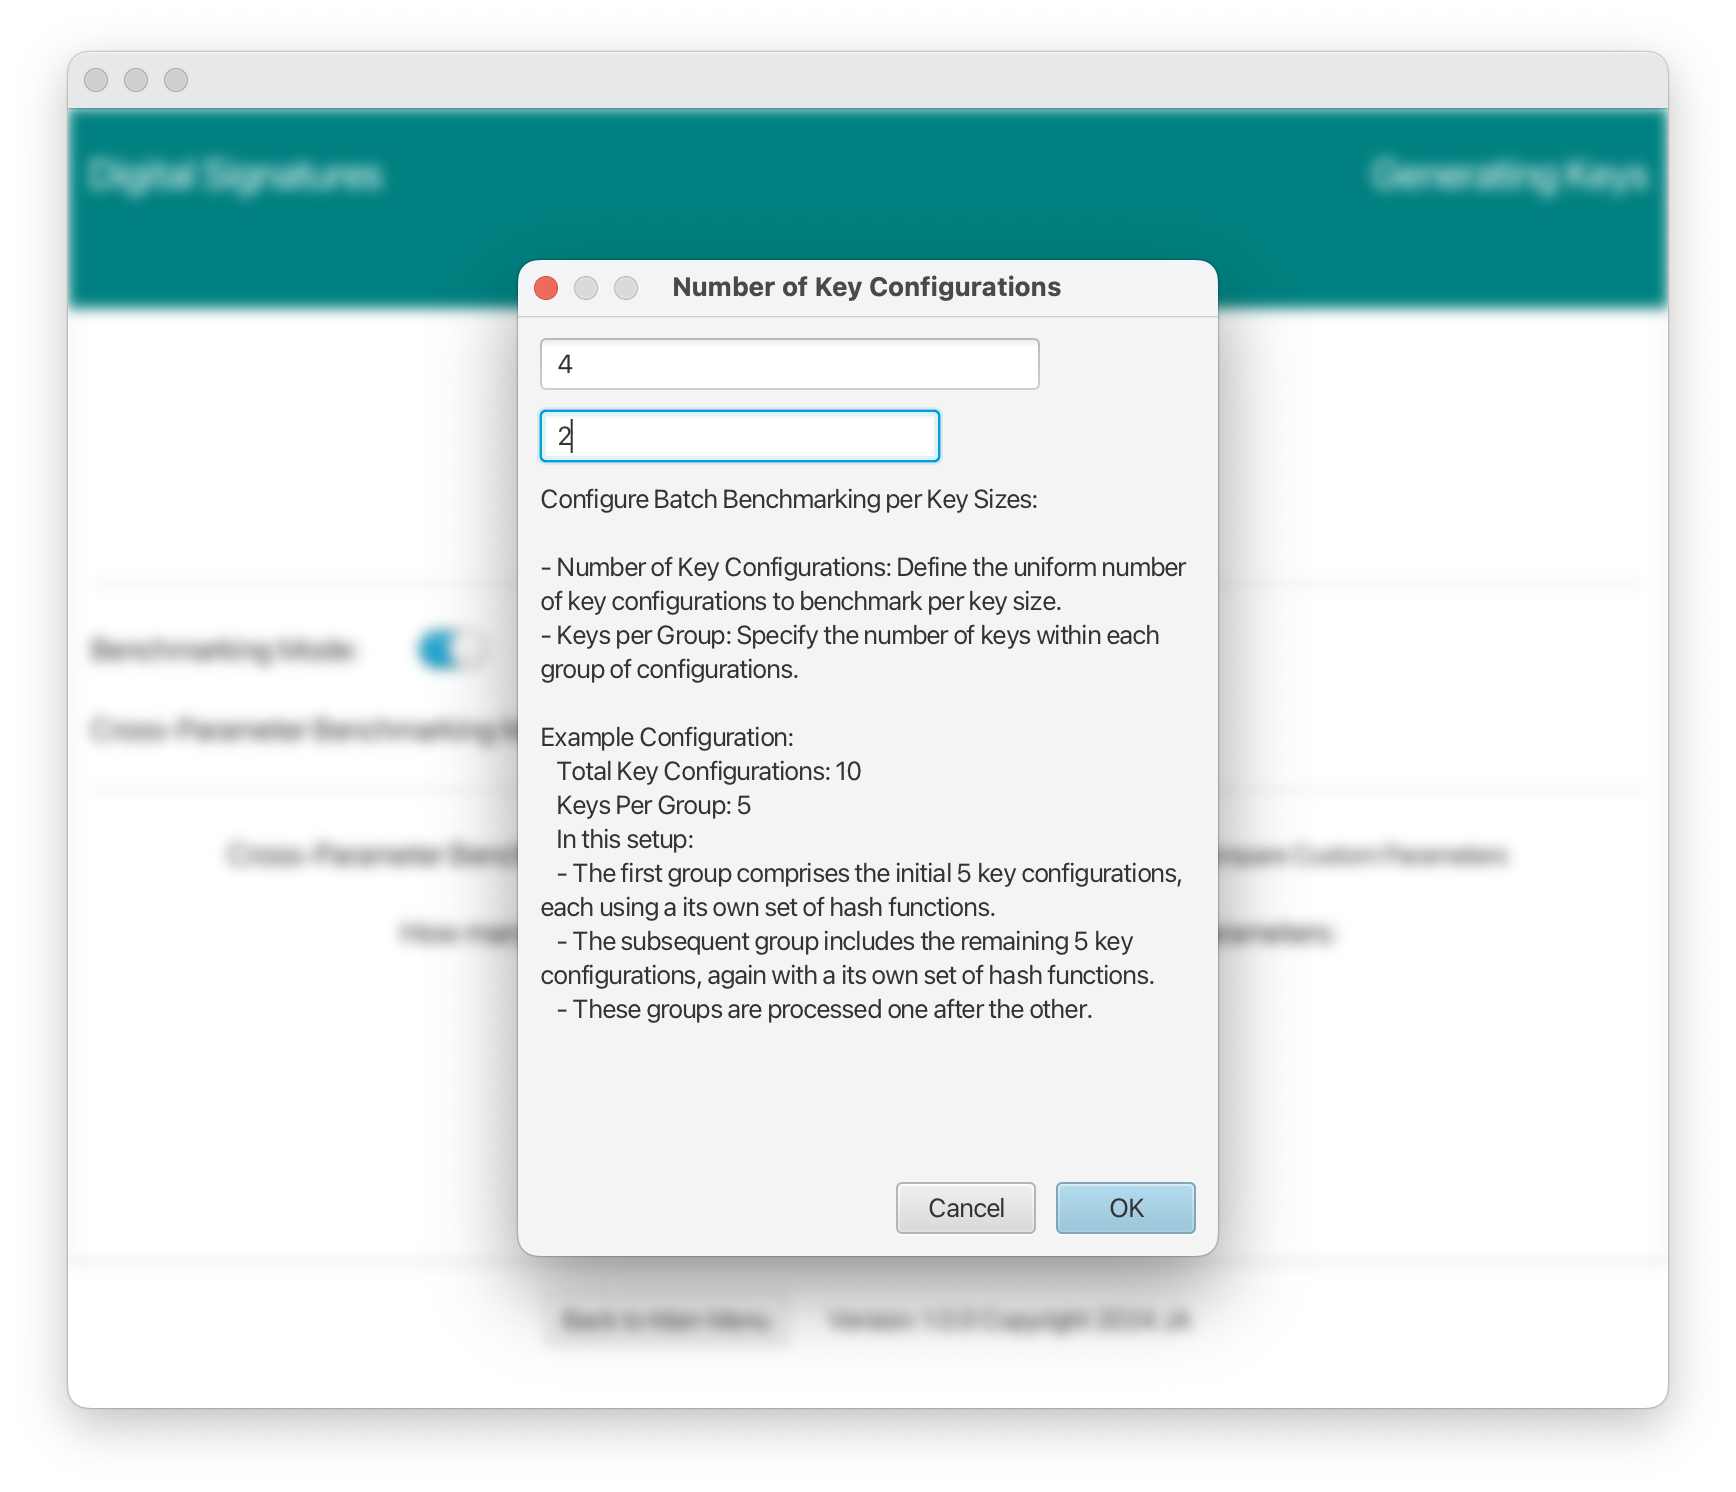
\includegraphics[width=\textwidth]{main_pictures/ui/custom3.png}
    \caption{Custom Comparison Benchmarking: Key Generation (number of key configurations)}
\end{figure}

After accepting key size the application displays a dialog for user to input the total number of key configurations to be benchmarked for each key size, alongside the number of keys in each configuration group. The number of keys within each group must be such that it evenly divides the total number of key configurations. For example, with ’Total Key Configurations: 4’ and ’Keys Per Group: 2’, the system will categorise the key configurations into two groups. Each group, comprising two key configurations, will be tested with its designated set of hash functions and applied to every key size.

\begin{figure}[H]
    \centering
    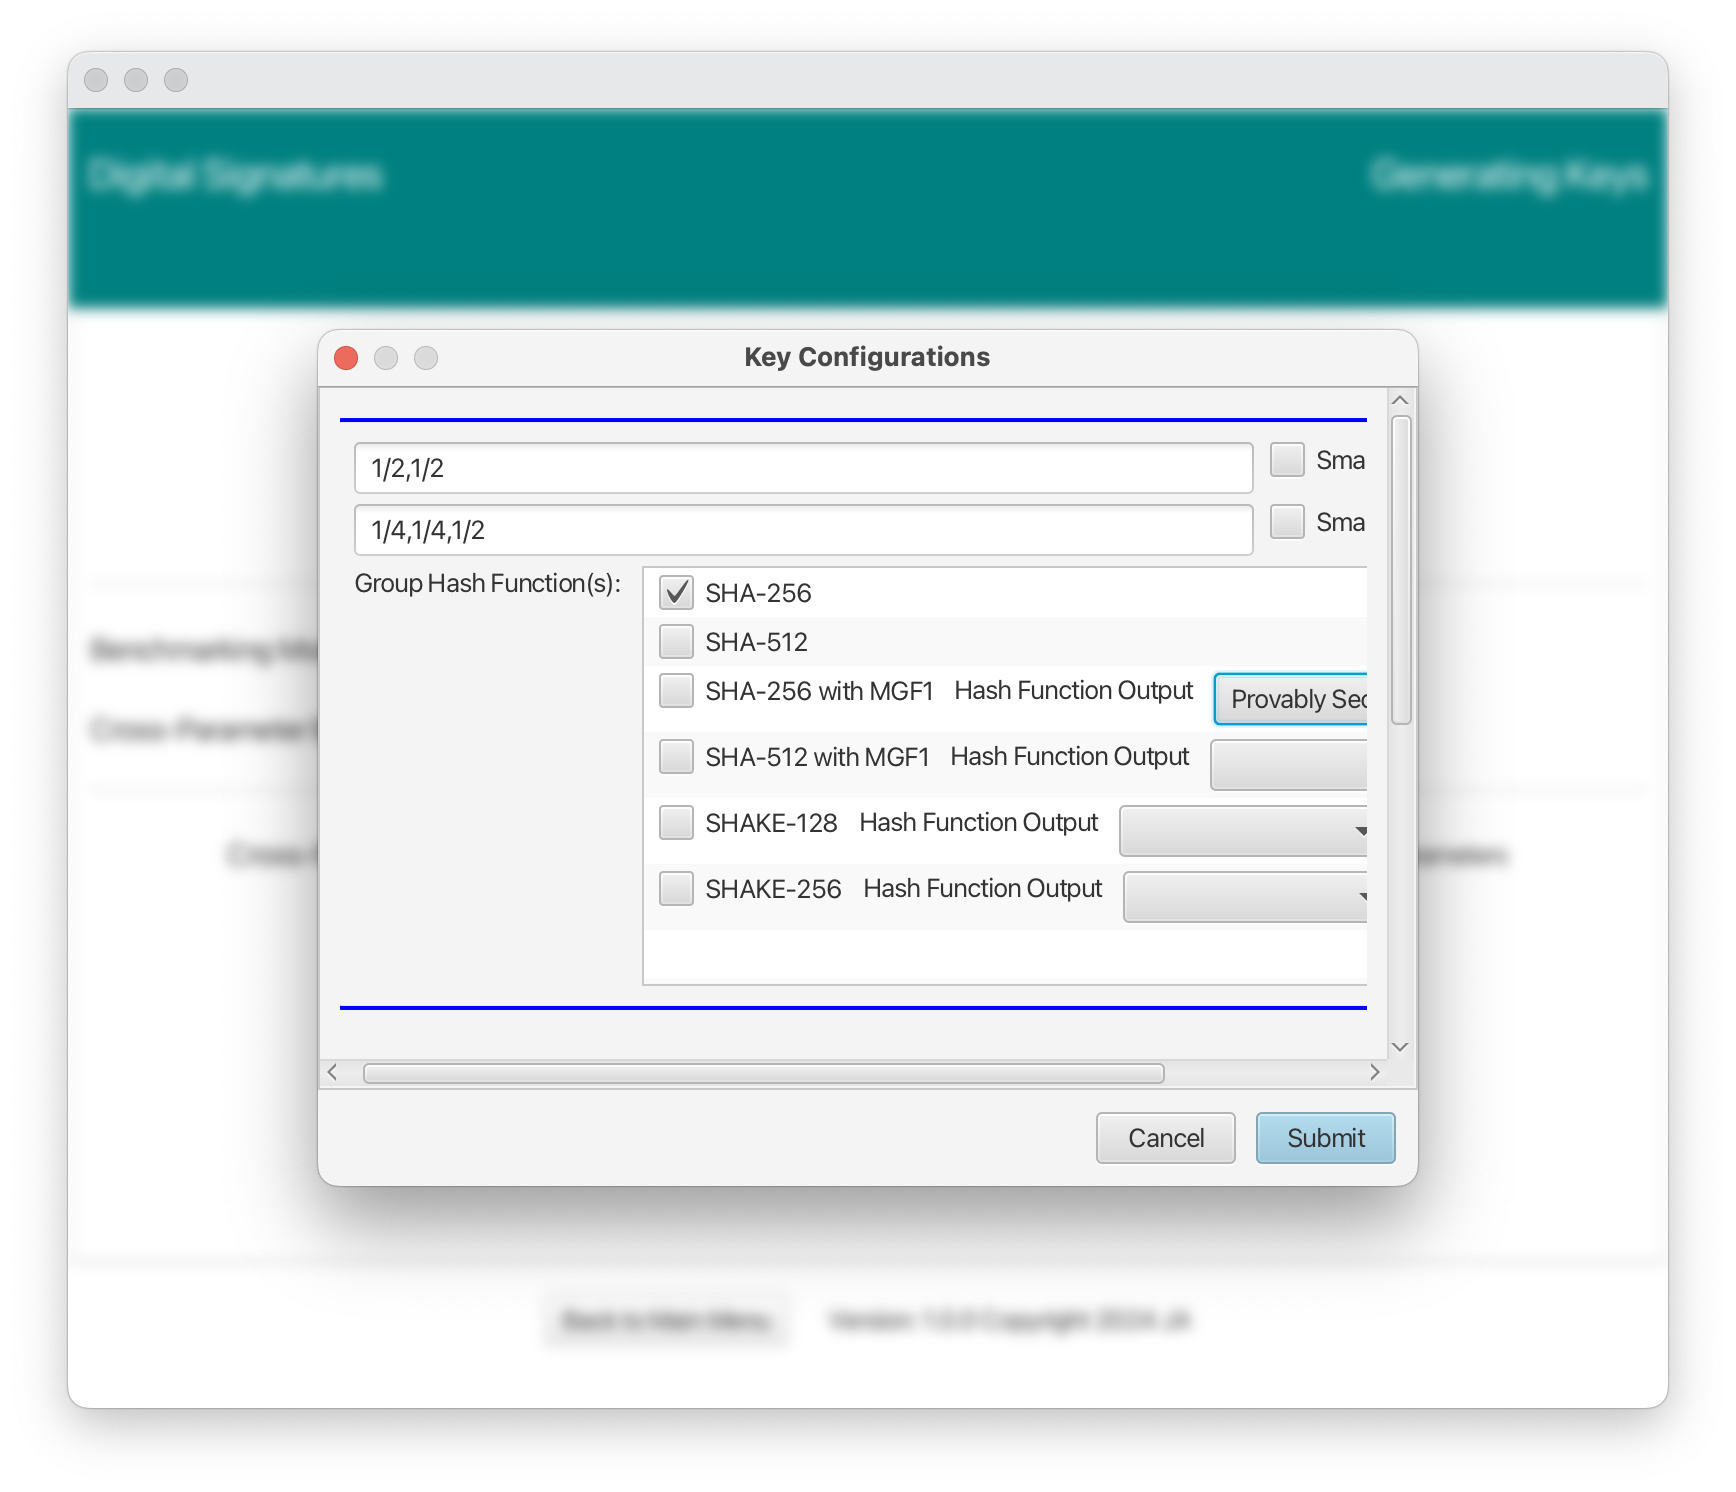
\includegraphics[width=\textwidth]{main_pictures/ui/custom4.png}
    \caption{Custom Comparison Benchmarking: Key Generation (key configurations (group 1))}
\end{figure}

\begin{figure}[H]
    \centering
    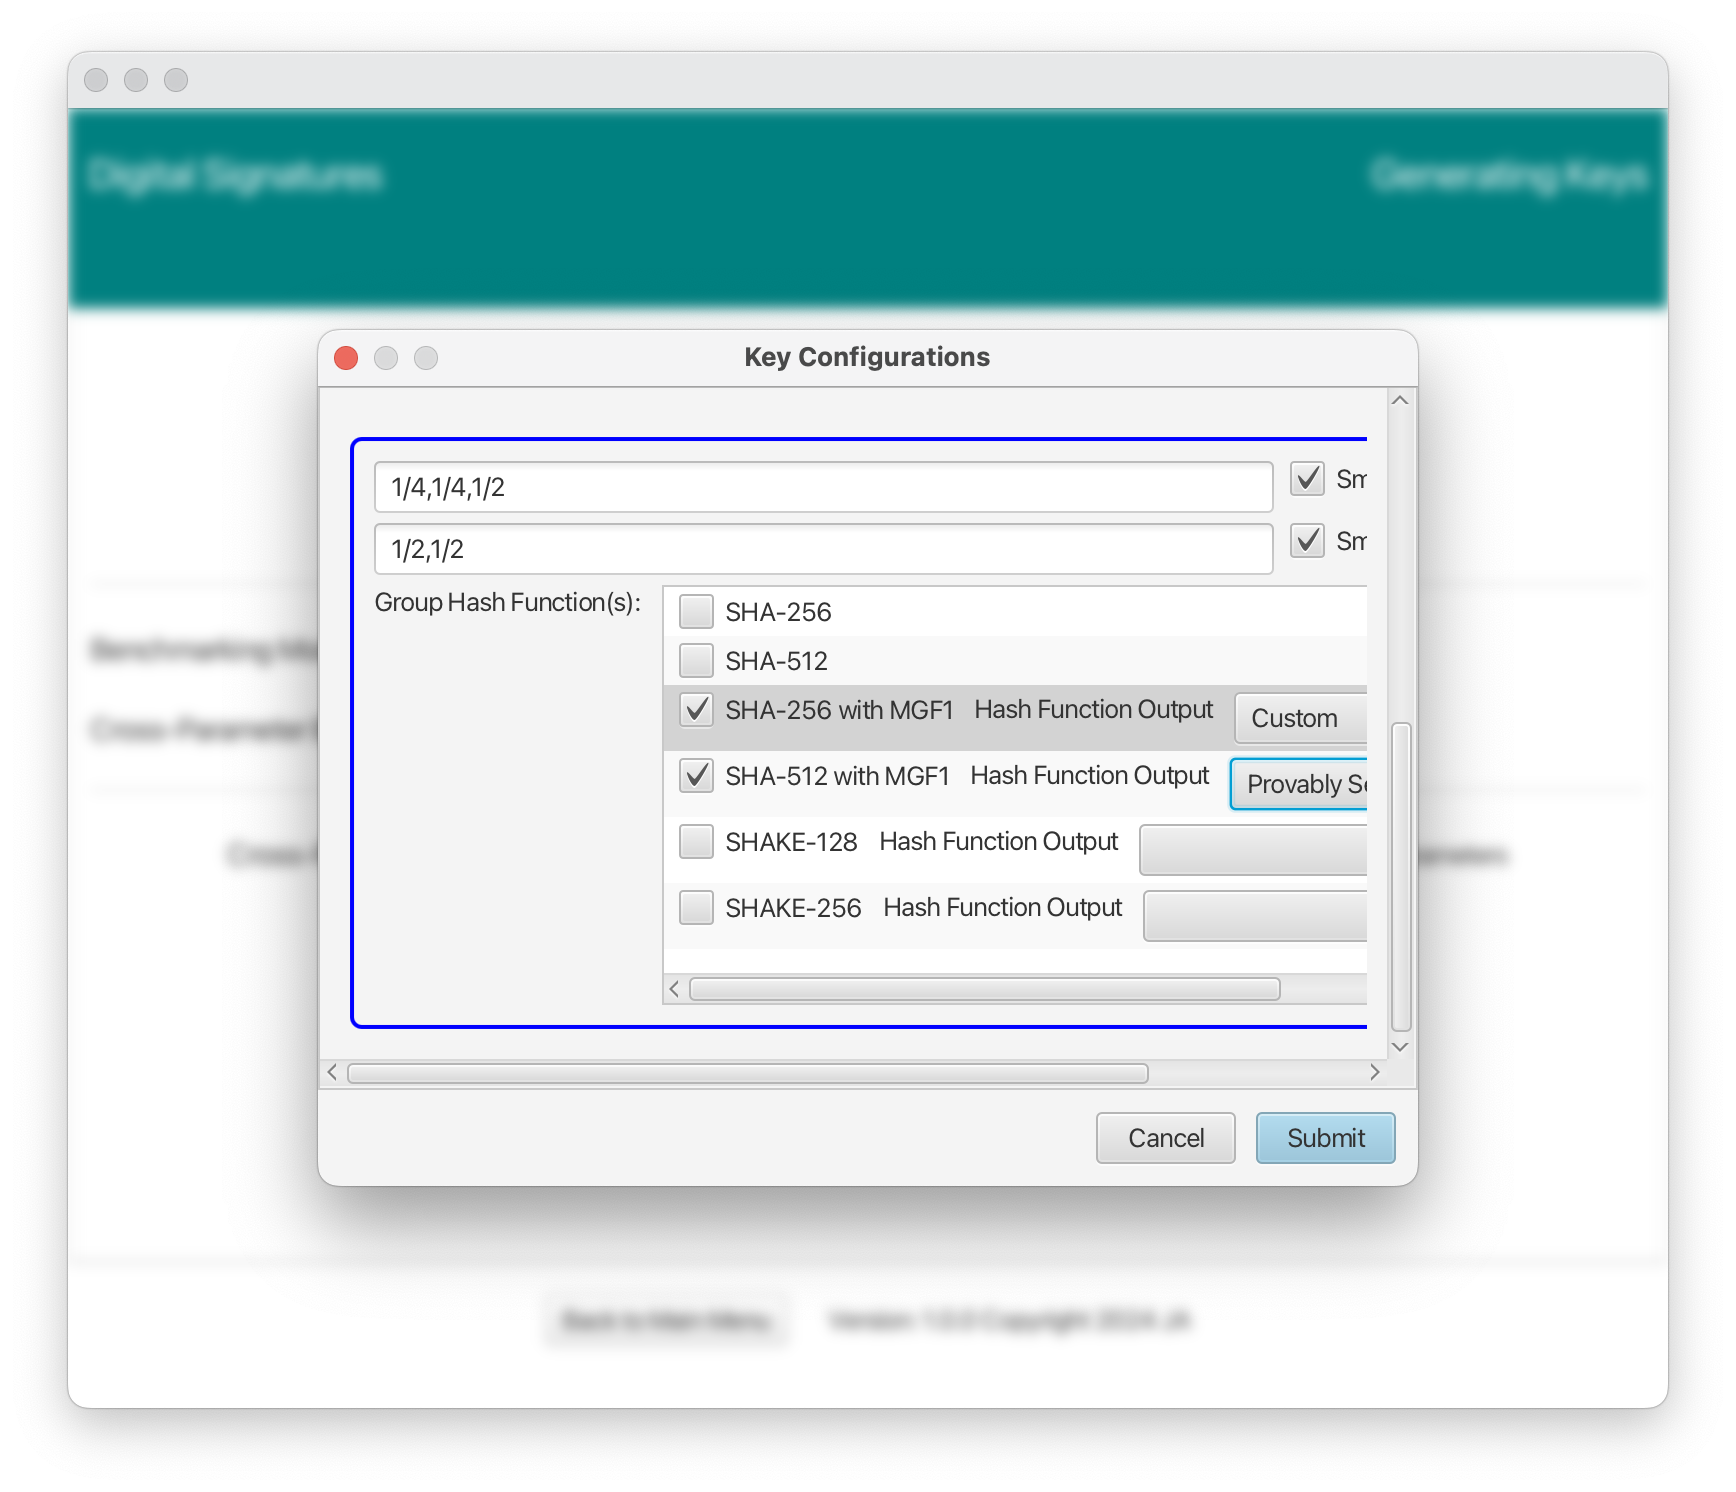
\includegraphics[width=\textwidth]{main_pictures/ui/custom5.png}
    \caption{Custom Comparison Benchmarking: Key Generation (key configurations (group 2))}
\end{figure}
For the setup of key configuration groups, the application presents elements corresponding to the number of groups previously specified. Within each group’s box:

\begin{itemize}
\item A series of text fields are available to define the prime factor distribution for each key configuration, with inputs expected as comma-separated fractional values (e.g., ’1/2, 1/4, 1/4’) that should collectively sum to 1, denoting the full key size.
Alongside each text field, users will find a checkbox to indicate whether they wish to use a small ’e’ value for generating that particular key configuration.
\item The concluding component within each group’s interface box is a multi- select list, populated with available hash functions. Users can select one or more hash functions by ticking the corresponding checkboxes. These selections apply the chosen set of hash functions to the key configurations within that group for subsequent signature related benchmarking activities.
\item Within the multi-select list interface for hash function selection, users  have the option to specify custom output lengths for variable-length hash functions facilitated by an adjacent dropdown menu for each hash function, labelled ”Hash Function Output Length.”
\end{itemize}


\begin{figure}[H]
    \centering
    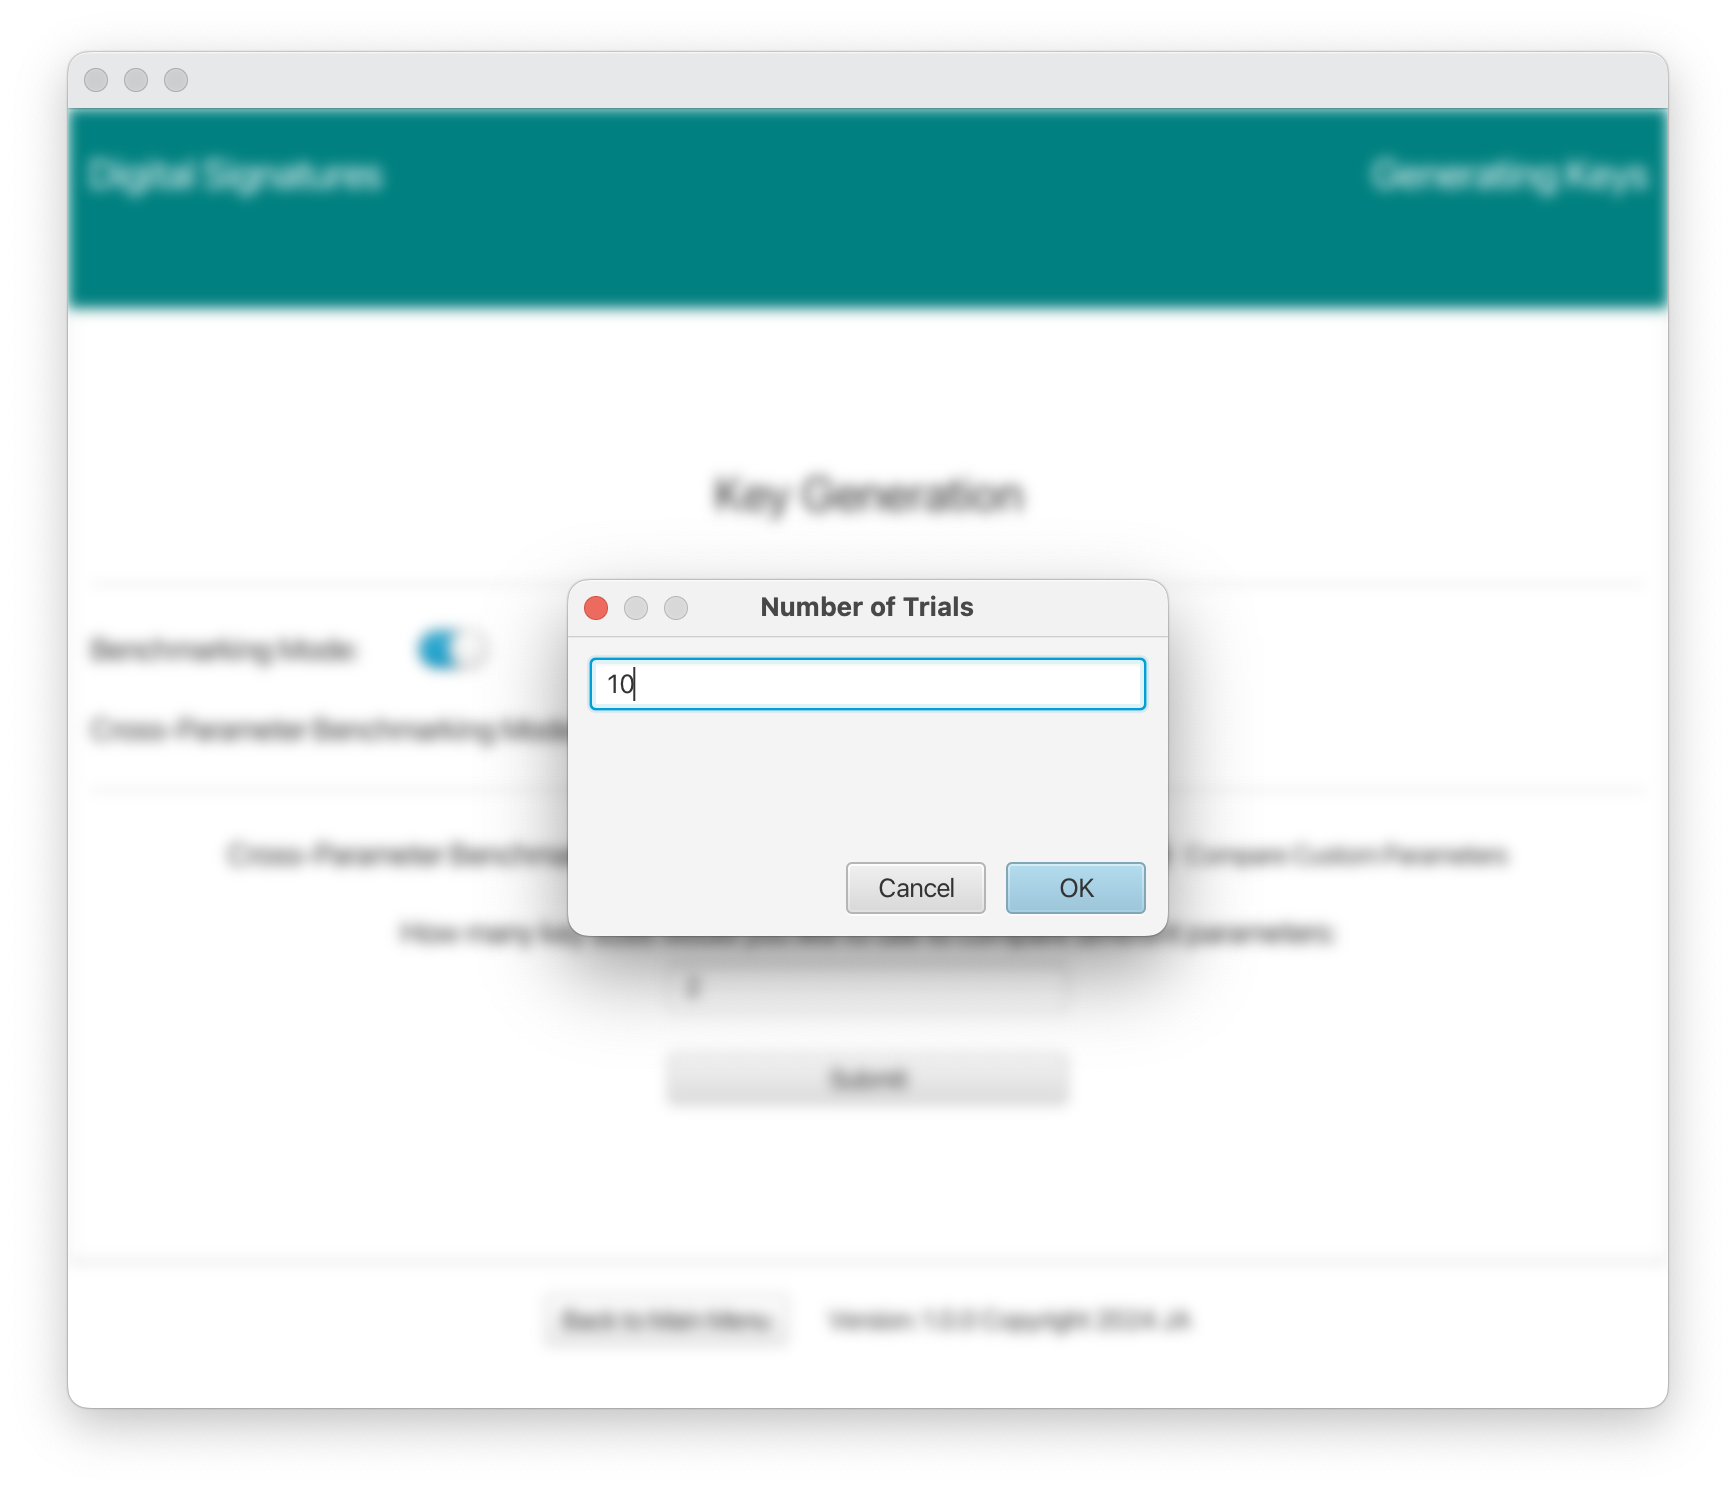
\includegraphics[width=\textwidth]{main_pictures/ui/custom6.png}
    \caption{Custom Comparison Benchmarking: Key Generation (number of trials)}
\end{figure}


Users then input the desired number of trials for key generation benchmarking, such as 10 trials. The application executes these trials for each of the key configurations specified at the selected key sizes.

Clicking the "OK" button on the number of trials dialog sets the benchmarking process in motion. A progress bar is displayed for a length of time spanning the duration of the task allowing for real-time indication of progress.


\begin{figure}[H]
    \centering
    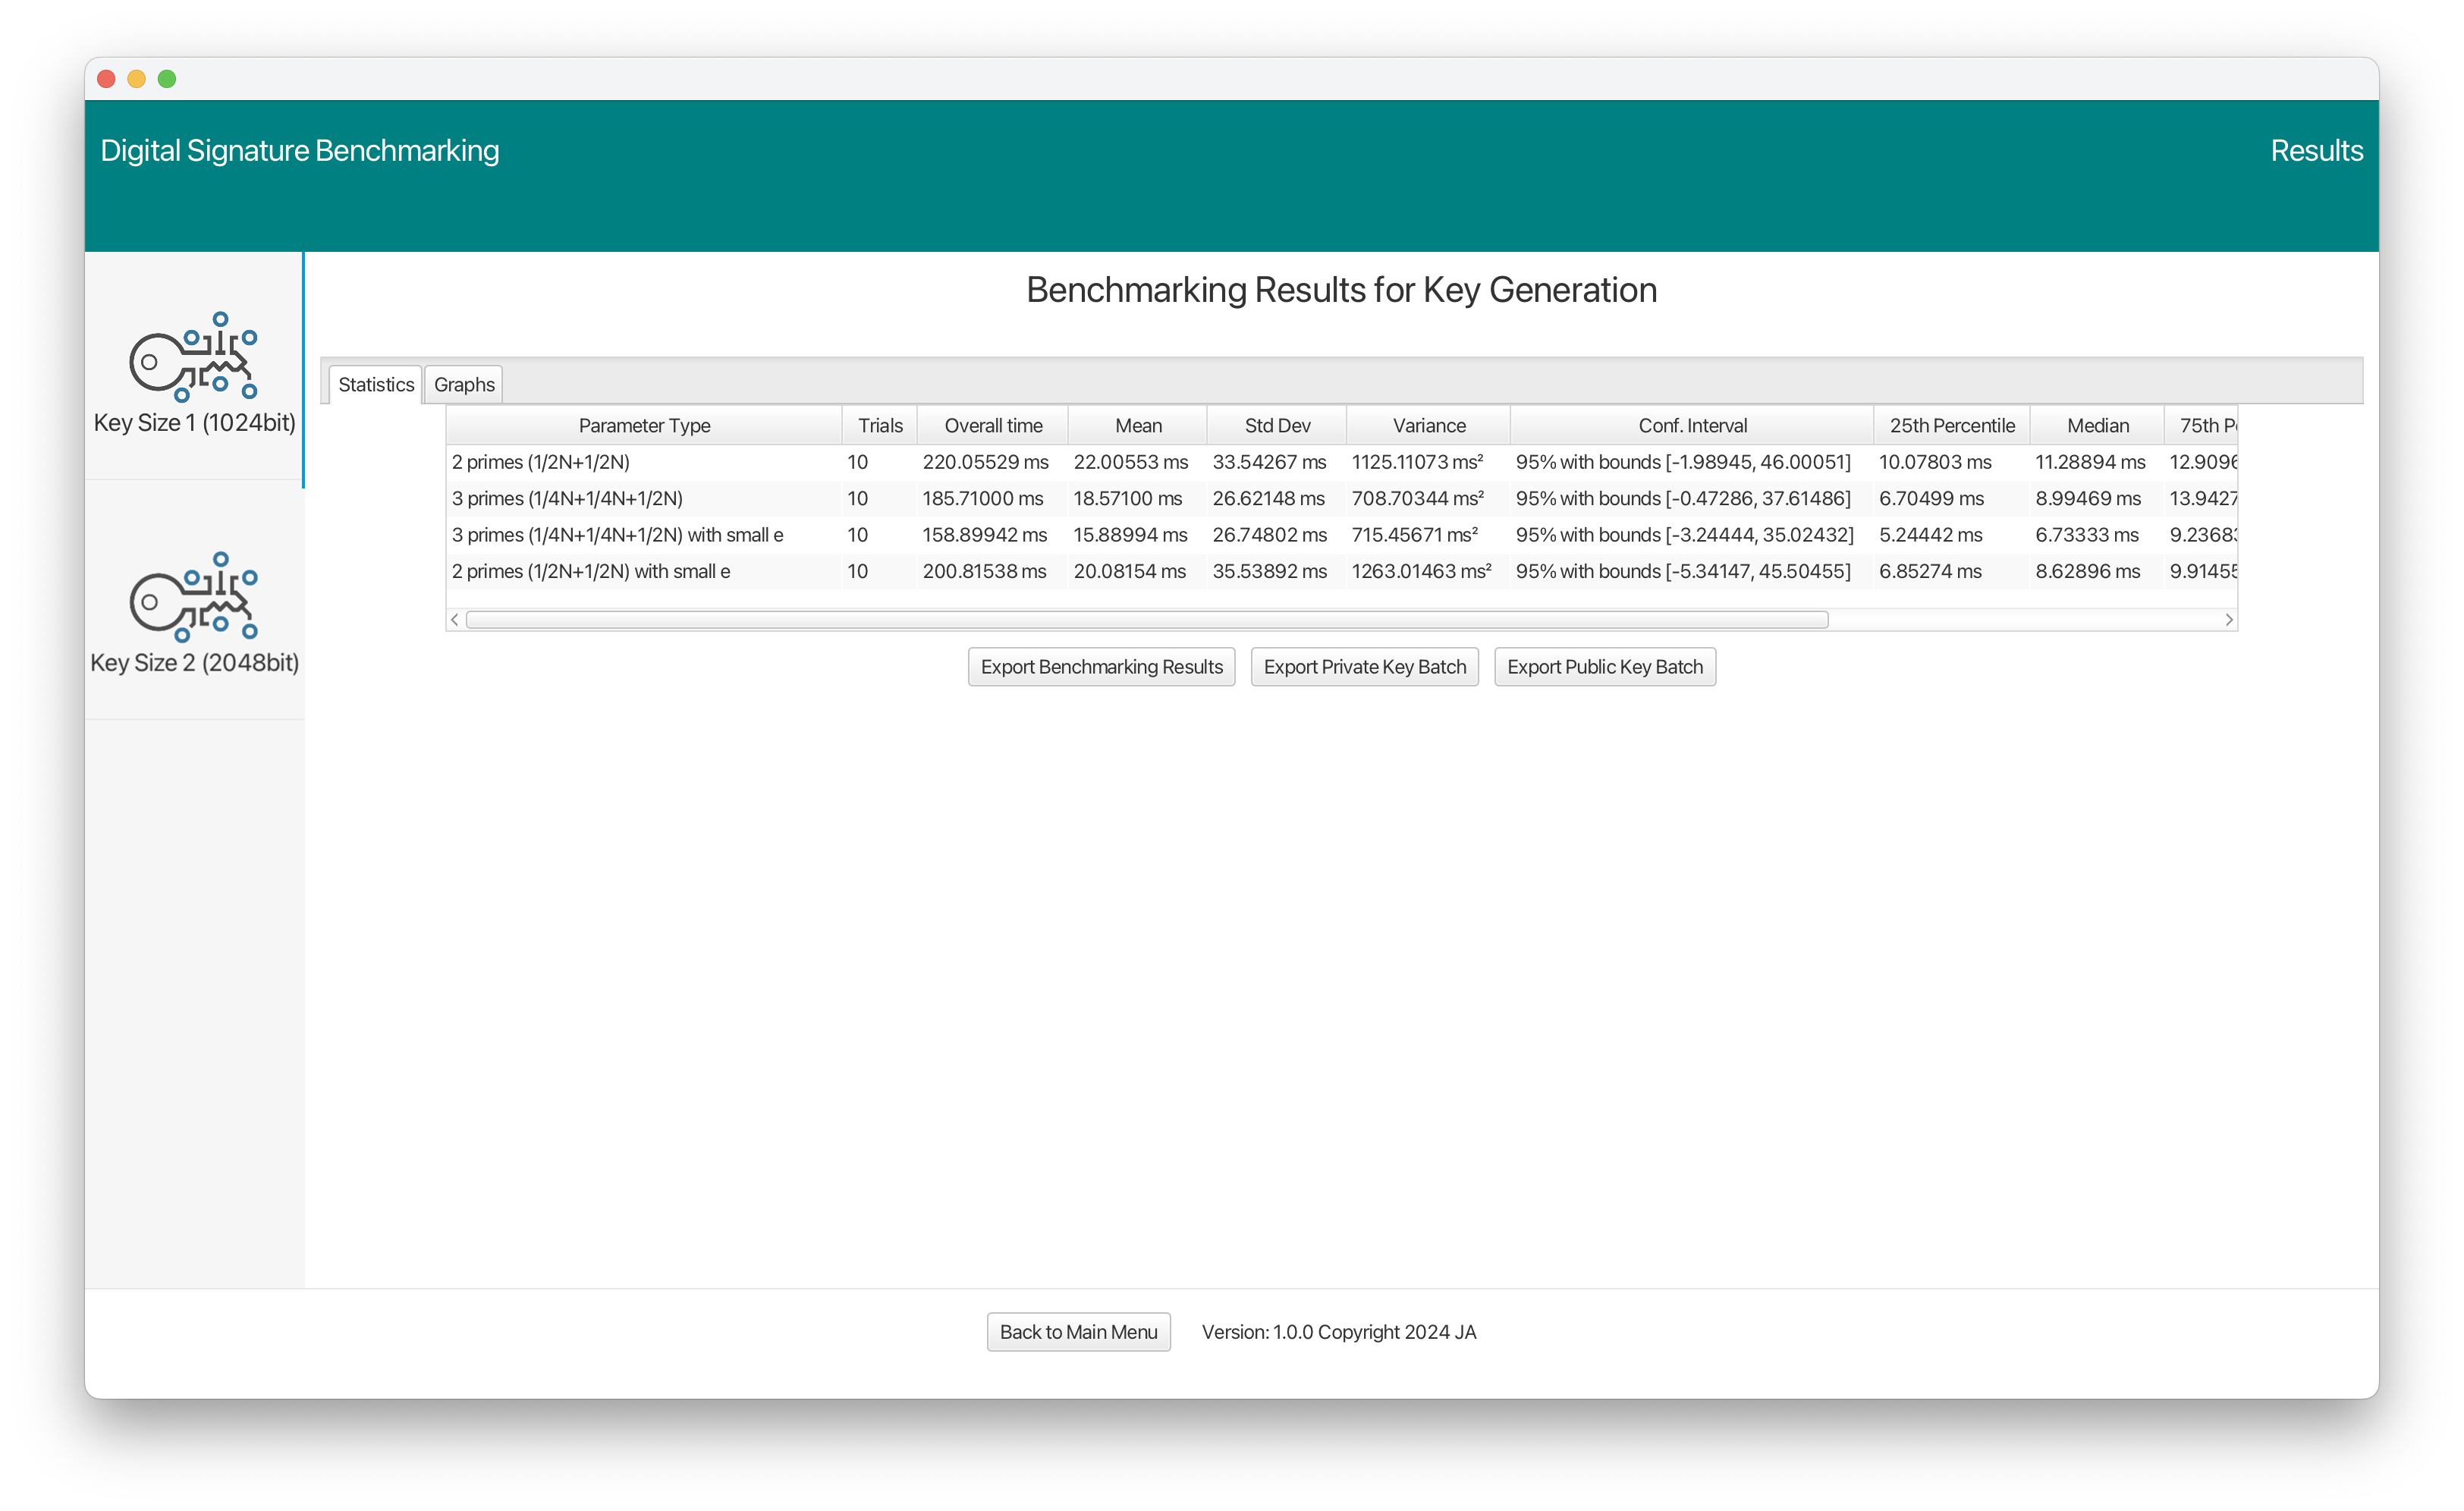
\includegraphics[scale= 0.325]{main_pictures/ui/custom7.png}
   \caption{Custom Comparison Benchmarking: Key Generation (Results Screen)}
\end{figure}
Upon completion of benchmarking, results from benchmarking are displayed. The results screen contains a side pane with buttons corresponding to each individual key size previously entered. Within each side tab, the results table displays a row by row sequence of statistical metrics for all entered key configurations.  The ordering is by parameter set (i.e., uniform number of key  configurations for each specified group in sequential order). Below the results table, the application also provides the functionality to export the benchmarking results and if desired public or private key batches corresponding to a global set of keys matching the key configurations enumerated in a sequence for all key sizes.


\subsection{Signature Generation}
\begin{figure}[H]
    \centering
    \includegraphics[scale= 0.4]{main_pictures/ui/custom8.png}
   \caption{Custom Comparison Benchmarking: Signature Generation (Custom Comparison Benchmarking)}
\end{figure}
The initial signature generation screen for Custom Comparison Benchmarking is activated by completing a key generation benchmarking run in comparison mode. On completion of this, the private key batch (and corresponding hash function choices) is preloaded into the signature creation portal. Thus when signature generation option is selected from the main menu, the Custom Comparison Benchmarking screen is displayed rather than the default benchmarking screen.
This explains the state of cross-parameter benchmarking toggle being set as switched on, as well as, specialised options appearing such as the application displaying a visual indication that a comparison-compatible private key batch was preloaded and the lack of hash function options since they were already specified

The signature creation screen is first organised with a pair of fields related to the importing of a message batch. There are specific requirements for the import of the message batch. 

The application expects the message batch as a non interrupted and new line separated sequence of messages and the number of lines must match the number entered in the adjacently above field. Otherwise import of a message batch is prevented.

On successful validation, the screen is updated with a checkmark indicator that provides visual confirmation that the message batch was successfully imported. The interface also includes a dropdown menu labeled signature scheme giving users the option to select the desired signature scheme  to be applied. 


Clicking "Start Signature Benchmarking" button initiates the execution the benchmarking task. This involves the creation of a batch of signatures for the message batch using the designated signature scheme and hash function-key combinations chosen during the key generation phase. A progress bar indicates progress in real time.

\textbf{Custom Comparison Benchmarking: Signature Generation Results Screen}


\begin{figure}[H]
    \centering
    \includegraphics[scale= 0.325]{main_pictures/ui/custom9.png}
   \caption{Custom Comparison Benchmarking: Signature Generation (Results Screen)}
\end{figure}

After completing signature generation benchmarking, results from benchmarking are displayed. The results screen features a side pane with tabs for each key size entered. Each tab reveals a results table displaying statistical metrics for all hash function-key combinations.
The table format aligns with the user's hash function choices. For the example scenario involving ’Total Key Configurations: 4’ and ’Keys Per Group: 2’, the results will display the first set of two key configurations for the initial group, followed by the subsequent two key configurations for the second group. This sequence will be laid out row by row per tab/key size.


Below the table, options are available to export benchmarking results and signature batches for each key size. The exported signature batch aligns with the key configurations and hash function combinations used, covering all key sizes in a single file.


\subsection{Signature Verification}

\begin{figure}[H]
    \centering
    \includegraphics[scale= 0.4]{main_pictures/ui/custom10.png}
   \caption{Custom Comparison Benchmarking: Signature Verification (Custom Comparison Benchmarking)}
\end{figure}

Similar to the process for signature generation, the signature verification screen for Custom Comparison Benchmarking is accessible after completing a key generation benchmark in custom comparison mode. This procedure also includes preloading a batch of keys and hash function selections. However, the key distinction lies in the type of key batch loaded. In the case of signature verification, it's a public key batch that gets preloaded, as opposed to a private key batch used for signature generation.

Aside from the preloaded public key batch and hash function selection used for Custom Comparison Benchmarking, the signature verification screen includes fields for importing both message and signature batches. For correctness, it's necessary that the submitted message batch aligns with the submitted signature batch. Moreover, these batches must be compatible with the public key batch, which, in turn, is associated with the private key batch employed during the prior signature generation phase.


Upon selecting "Start Verification Benchmarking," the application validates the number of signatures against the message batch and chosen hash functions.  Following successful validation,  verification benchmarking is executed . This involves comparing the signature batch with the message batch and public keys, using the selected signature scheme and hash functions. The process generates batches of verification results for each entered key size, and a progress bar provides real-time progress updates.

\newpage
\textbf{Custom Comparison Benchmarking: Signature Verification Results Screen}

\begin{figure}[H]
    \centering
    \includegraphics[scale= 0.325]{main_pictures/ui/custom11.png}
   \caption{Custom Comparison Benchmarking: Signature Verification (Results Screen)}
\end{figure}

Once the signature verification benchmarking concludes, results from benchmarking are displayed. The layout of this results screen is largely as was shown for signature generation. The distinction is the enabling of the export of verification results for each key size. displayed below each results table.




\chapter{Additional Features}

\section{All benchmarking modes: Signature Processing for Message Recovery Schemes}

In the Signature processes, when utilising the message recovery ISO/IEC 9796-2 Scheme, there is a specific approach for handling non-recoverable portion when signature generation is performed and recovered portion of messages when signature verification is performed. 

Although the following outlines the procedure in comparison benchmarking, the equivalent mechanism applies for all other modes.
\begin{figure}[H]
    \centering % Center the images
    
    % First image in a minipage
    \begin{minipage}{0.2\textwidth}
        \centering
        \fbox{\includegraphics[width=\textwidth]{main_pictures/ui/signing/signing2.png}} % Adding border here
       \caption{Comparison Benchmarking: Signature Creation (Test message batch (testMessages.txt))}

        \label{fig:image1}
    \end{minipage}
    \hfill % Add some space between the images
    % Second image in a minipage
    \begin{minipage}{0.7\textwidth}
        \centering
         \fbox{\includegraphics[width=\textwidth]{main_pictures/ui/signing/signing11.png}} % Adding border here
       \caption{Comparison Benchmarking: Signature Generation with ISO scheme selected}        \label{fig:image2}
    \end{minipage}
    
      \begin{minipage}{0.7\textwidth}
        \centering
         \fbox{\includegraphics[width=\textwidth]{main_pictures/ui/signing/signing12.png}} % Adding border here
       \caption{Comparison Benchmarking: Signature Generation Results Screen (with Message Recovery Options)}        \label{fig:image2}
    \end{minipage}
\end{figure}

For signature generation this process involves exporting a batch of non-recoverable messages where each line corresponds with a signature. Lines are prefixed with a "1" to indicate the presence of a non-recoverable message and "0" when there is none. In this specific case, since all messages are too short to produce a non-recoverable part regardless of the key sizes selected, the resulting file comprises a sequence of "0" flags, each separated by a new line.


\begin{figure}[H]
    \centering
    \includegraphics[width=\textwidth]{main_pictures/ui/verifying/verifying10.png}
   \caption{Comparison Benchmarking: Signature verification with ISO scheme selected}
\end{figure}

The corresponding verification of signatures necessitates import of a non-recoverable message batch file generated from the preceding signature generation benchmarking process. As discussed it contains entries aligned with each signature, organised line by line where each entry starts with a "1" or "0" flag, indicating whether a non-recoverable message part is present or absent, respectively. The application then leverages these non-recoverable message parts, to construct the content of a recovered message batch. This information is then displayed as a dedicated column in the verification Results CSV files, which users can export for further analysis.


\section{Standard mode: Signature Processing for Message Recovery Schemes}

When using a signature scheme that supports message recovery, such as ISO/IEC 9796-2 Scheme 1, and a part of the document is non-recoverable (cannot be reconstructed solely from the signature), the notification panel presents further relevant options for exporting.

\begin{figure}[H]
    \centering % Center the images
    
    % First image in a minipage
    \begin{minipage}{0.49\textwidth}
        \centering
        \fbox{\includegraphics[width=\textwidth]{main_pictures/ui/signing/standard/signing1.png}} % Adding border here
       \caption{Standard Mode: Signature Creation with ISO scheme selected}
        \label{fig:image1}
    \end{minipage}
    \hfill % Add some space between the images
    % Second image in a minipage
    \begin{minipage}{0.49\textwidth}
        \centering
        \fbox{\includegraphics[width=\textwidth]{main_pictures/ui/signing/standard/signing2.png}} % Adding border here
       \caption{Standard Mode: Signature Creation with message recovery options}
        \label{fig:image2}
    \end{minipage}
\end{figure}

When using a message recovery-type signature scheme like ISO/IEC 9796-2 Scheme 1, successful signature verification allows for the recovered message to be exported. Notably, verifying an ISO/IEC 9796-2 Scheme 1 signature does not require the original text input in cases of full message recovery. This is because the goal of verification here is to extract the complete message initially fed into the signature generation process from the signature itself.

\begin{figure}[H]
    \centering % Center the images
    
    % First image in a minipage
    \begin{minipage}{0.49\textwidth}
        \centering
        \fbox{\includegraphics[width=\textwidth]{main_pictures/ui/verifying/standard/verifying1.png}} % Adding border here
       \caption{Standard Mode: Signature Creation with ISO scheme selected}
        \label{fig:image1}
    \end{minipage}
    \hfill % Add some space between the images
    % Second image in a minipage
    \begin{minipage}{0.49\textwidth}
        \centering
        \fbox{\includegraphics[width=\textwidth]{main_pictures/ui/verifying/standard/verifying2.png}} % Adding border here
       \caption{Standard Mode: Signature Creation with message recovery options}
        \label{fig:image2}
    \end{minipage}
\end{figure}


\section{Benchmarking mode: Preloading a provably secure key batch for Signature creation/verification}

\begin{figure}[H]
    \centering % Center the images
    
    % First image in a minipage
    \begin{minipage}{0.49\textwidth}
        \centering
        \fbox{\includegraphics[width=\textwidth]{main_pictures/preload1.png}} % Adding border here
       \caption{Benchmarking: Key Generation (With Small e option selected for keys)}
        \label{fig:pre1}
    \end{minipage}
    \hfill % Add some space between the images
    % Second image in a minipage
    \begin{minipage}{0.49\textwidth}
        \centering
        \fbox{\includegraphics[width=\textwidth]{main_pictures/preload2.png}} % Adding border here
       \caption{Benchmarking: Signature Creation (Preloaded provably secure private key batch)}
        \label{fig:pre2}
    \end{minipage}
      \begin{minipage}{0.55\textwidth}
        \centering
        \fbox{\includegraphics[width=1.2\textwidth]{main_pictures/preload3.png}} % Adding border here
       \caption{Benchmarking: Signature Verification (Preloaded provably secure private key batch)}
        \label{fig:pre3}
    \end{minipage}
\end{figure}

The above images outlines the steps taken by a user within the system to preload a provably secure key batch to allow for an application confirmed instantiation of signature schemes with provably secure parameters



As before the process begins when the user inputs the key configurations, indicating the desired key size and whether to utilise a small public exponent (e) for each key. However an alternate path is followed in \ref{fig:pre1} where the option for a small e was specified for all key configurations. The system then proceeds to generate a batch of key pairs and benchmarks the key generation process, provided the key sizes and options are valid. A further step in this case is that the application preloads the provably secure key batches into signature creation and signature verification portals.



This means the private key batch/public key batches are preloaded into the signature creation and verification portals respectively. Thus when either signature option is selected from the main menu, a specialised view of the benchmarking screen is displayed rather than the default benchmarking screen.
This explains the application displaying a visual indication that a provably secure key batch was preloaded in both cases, as well as a specialised radio button option appearing labelled "Instantiate Scheme with provably secure parameters". Since the application knows the key batch is provably secure (small e option selected for all keys), it can provide a verified instantiation of the signature scheme with provably secure parameters on the condition that a provably secure hash size is also selected, hence the additional restriction on hash function size.  

The same mechanism is also in place for single keys when standard mode is active.


\end{document}

\end{article}
